%% abtex2-modelo-trabalho-academico.tex, v-1.7.1 laurocesar
%% Copyright 2012-2013 by abnTeX2 group at http://abntex2.googlecode.com/
%%
%% This work may be distributed and/or modified under the
%% conditions of the LaTeX Project Public License, either version 1.3
%% of this license or (at your option) any later version.
%% The latest version of this license is in
%%   http://www.latex-project.org/lppl.txt
%% and version 1.3 or later is part of all distributions of LaTeX
%% version 2005/12/01 or later.
%%
%% This work has the LPPL maintenance status `maintained'.
%%
%% The Current Maintainer of this work is the abnTeX2 team, led
%% by Lauro C\'{e}sar Araujo. Further information are available on
%% http://abntex2.googlecode.com/
%%
%% This work consists of the files abntex2-modelo-trabalho-academico.tex,
%% abntex2-modelo-include-comandos and abntex2-modelo-references.bib
%%

% ------------------------------------------------------------------------
% ------------------------------------------------------------------------
% abnTeX2: Modelo de Trabalho Academico (tese de doutorado, dissertacao de
% mestrado e trabalhos monograficos em geral) em conformidade com
% ABNT NBR 14724:2011: Informacao e documentacao - Trabalhos academicos -
% Apresentacao
% ------------------------------------------------------------------------
% ------------------------------------------------------------------------

%ARQUIVO DE PREAMBULO DA TESE - PACOTES E CONFIGURA\c{C}\~{O}ES

\documentclass[
	% -- op\c{c}\~{o}es da classe memoir --
	12pt,				% tamanho da fonte
    % 	openright,			% cap\'{\i}tulos come\c{c}am em p\'{a}g \'{\i}mpar (insere p\'{a}gina vazia caso preciso)
	oneside,			% para impress\~{a}o em verso e anverso. Oposto a oneside/twoside
	letterpaper,		% tamanho do papel.
	% -- op\c{c}\~{o}es da classe abntex2 --
	%chapter=TITLE,		% t\'{\i}tulos de cap\'{\i}tulos convertidos em letras mai\'{u}sculas
	%section=TITLE,		% t\'{\i}tulos de se\c{c}\~{o}es convertidos em letras mai\'{u}sculas
	%subsection=TITLE,	% t\'{\i}tulos de subse\c{c}\~{o}es convertidos em letras mai\'{u}sculas
	%subsubsection=TITLE,% t\'{\i}tulos de subsubse\c{c}\~{o}es convertidos em letras mai\'{u}sculas
	% -- op\c{c}\~{o}es do pacote babel --
	% brazil,			% idioma adicional para hifeniza\c{c}\~{a}o
	%french,			% idioma adicional para hifeniza\c{c}\~{a}o
	%spanish,			% idioma adicional para hifeniza\c{c}\~{a}o
	english,			% o \'{u}ltimo idioma \'{e} o principal do documento
	sumario=tradicional,
% 	sumario=abnt-6027-2012,
    oldfontcommands,
	]{abntex2}

\renewcommand{\ABNTEXchapterfont}{\fontfamily{cmr}\selectfont}
\renewcommand{\ABNTEXchapterfontsize}{\HUGE}

% ---
% PACOTES
% ---

% ---
% Pacotes fundamentais
% ---
\usepackage{cmap}				% Mapear caracteres especiais no PDF
% \usepackage{lmodern}			% Usa a fonte Latin Modern			
\usepackage[T1]{fontenc}		% Selecao de codigos de fonte.
\usepackage[utf8]{inputenc}		% Codificacao do documento (convers\~{a}o autom\'{a}tica dos acentos)
\usepackage{lastpage}			% Usado pela Ficha catalogr\'{a}fica
\usepackage{indentfirst}		% Indenta o primeiro par\'{a}grafo de cada se\c{c}\~{a}o.
\usepackage{color}				% Controle das cores
\usepackage[pdftex]{graphicx}	% Inclus\~{a}o de gr\'{a}ficos
\usepackage{epstopdf}           % Pacote que converte as figuras em eps para pdf
% \usepackage{lipsum}             % Pacote que gera texto dummy
% \usepackage{blindtext}          % Pacote que gera texto dummy
% ---
		
% ---
% Pacotes adicionais, usados apenas no \^{a}mbito do Modelo Can\^{o}nico do abnteX2
% ---
\usepackage{nomencl}
\usepackage{amssymb,amsfonts,amsthm,amsmath,mathrsfs,bbm,bm,dsfont,etoolbox}
\usepackage[chapter]{algorithm}
\usepackage{algorithmic}
\usepackage{multirow}
\usepackage{rotating}
\usepackage{pdfpages}
% ---


% ---
% Pacotes de cita\c{c}\~{o}es
% ---
\usepackage[brazilian,hyperpageref]{backref}	 % Paginas com as cita\c{c}\~{o}es na bibl
\usepackage[alf,abnt-etal-cite=2,abnt-etal-list=0,abnt-etal-text=emph]{abntex2cite}	% Cita\c{c}\~{o}es padr\~{a}o ABNT

% ---
% Pacote de customiza\c{c}\~{a}o - Unicamp
% ---
\usepackage{unicamp}

% Pacotes adicionais
\usepackage{tikz}
\usetikzlibrary{calc}
\usepackage{pgfplots}
\pgfplotsset{compat=1.7}
\usepgfplotslibrary{fillbetween}
\usetikzlibrary{arrows.meta}
\def\arrowhead{Latex[length=3mm, width=1.5mm]}

\usepackage{caption, subcaption}
\usepackage{enumitem}
\usepackage{empheq}

\usepackage{chngcntr}
\counterwithin{figure}{chapter}
\counterwithin{table}{chapter}

%Options: Sonny, Lenny, Glenn, Conny, Rejne, Bjarne, Bjornstrup
\usepackage[Lenny]{fncychap}
% ---
% CONFIGURA\c{C}\~{O}ES DE PACOTES
% ---
% \def\labelitemi{--} % configura bullets do Itemize
\def\labelitemi{\bf --}

% \patchcmd{\endproof}% <cmd> % coloca linha no fim de proof
%   {\endtrivlist}% <search>
%   {\endtrivlist\par\nobreak\vspace*{\dimexpr-\baselineskip-\parskip}\nobreak\noindent\hrulefill}% <replace>
%   {}{}% <succes><failure>

% ---
% Configura\c{c}\~{o}es do pacote backref
% Usado sem a op\c{c}\~{a}o hyperpageref de backref
\graphicspath{{./eps/}}
\DeclareGraphicsExtensions{.eps}

%customiza\c{c}\~{a}o do negrito em ambientes matem\'{a}ticos
\newcommand{\mb}[1]{\mathbf{#1}}
%customiza\c{c}\~{a}o de teoremas
% \newtheorem{mydef}{Defini\c{c}\~{a}o}[chapter]
% \newtheorem{lemm}{Lema}[chapter]
% \newtheorem{theorem}{Teorema}[chapter]
\floatname{algorithm}{Pseudoc\'{o}digo}
\renewcommand{\listalgorithmname}{Lista de Pseudoc\'{o}digos}


% \renewcommand{\backrefpagesname}{Citado na(s) p\'{a}gina(s):~}
% % Texto padr\~{a}o antes do n\'{u}mero das p\'{a}ginas
% \renewcommand{\backref}{}
% % Define os textos da cita\c{c}\~{a}o
% \renewcommand*{\backrefalt}[4]{
% 	\ifcase #1 %
% 		Nenhuma cita\c{c}\~{a}o no texto.%
% 	\or
% 		Citado na p\'{a}gina #2.%
% 	\else
% 		Citado #1 vezes nas p\'{a}ginas #2.%
% 	\fi}%
% % ---

\renewcommand{\backrefpagesname}{Cited in page(s):~}
% Texto padr\~{a}o antes do n\'{u}mero das p\'{a}ginas
\renewcommand{\backref}{}
% Define os textos da cita\c{c}\~{a}o
\renewcommand*{\backrefalt}[4]{
	\ifcase #1 %
		No citations in the text.%
	\or
		Cited in page #2.%
	\else
		Cited #1 times in pages #2.%
	\fi}%
% ---

% ---
% Configura\c{c}\~{o}es de apar\^{e}ncia do PDF final

% alterando o aspecto da cor azul
\definecolor{blue}{RGB}{41,5,195}

% informa\c{c}\~{o}es do PDF
\makeatletter
\hypersetup{
     	%pagebackref=true,
		pdftitle={\@title},
		pdfauthor={\@author},
    	pdfsubject={\imprimirpreambulo},
	    pdfcreator={LaTeX with abnTeX2},
		pdfkeywords={abnt}{latex}{abntex}{abntex2}{trabalho acad\^{e}mico},
		hidelinks,					% desabilita as bordas dos links
		colorlinks=false,       	% false: boxed links; true: colored links
    	linkcolor=blue,          	% color of internal links
    	citecolor=blue,        		% color of links to bibliography
    	filecolor=magenta,      	% color of file links
		urlcolor=blue,
%		linkbordercolor={1 1 1},	% set to white
		bookmarksdepth=4
}
\makeatother
% ---

% ---
% Espa\c{c}amentos entre linhas e par\'{a}grafos
% ---

% O tamanho do par\'{a}grafo \'{e} dado por:
\setlength{\parindent}{20pt}
% \setlength{\parindent}{2cm}

% Controle do espa\c{c}amento entre um par\'{a}grafo e outro:
\setlength{\parskip}{0.2cm}  % tente tamb\'{e}m \onelineskip

% ---
% Informacoes de dados para CAPA e FOLHA DE ROSTO
% ---
\titulo{Spatio-temporal Traffic in\\[0ex] Interference Networks\\[7ex]
Tráfego Espaço-temporal em\\[4mm] Redes de Interferência}
% \tituloestrangeiro{Tráfego Espaço-temporal em Redes de Interferência}
\autor{Pl\'{i}nio Santini Dester}
\local{Campinas}
\data{2021}
\orientador[\textbf{Orientador:}]{Prof. Dr. Paulo Cardieri}
% \coorientador[Co-orientador]{Prof. Dr. Co-orientador}
\instituicao{%
    Universidade Estadual de Campinas
    \par
    Faculdade de Engenharia El\'{e}trica e de Computa\c{c}\~{a}o
    }
%\tipotrabalho{Tese (Doutorado)}
%% O preambulo deve conter o tipo do trabalho, o objetivo, o nome da institui\c{c}\~{a}o e a \'{a}rea de concentra\c{c}\~{a}o
%\preambulo{Tese apresentada \`{a} Faculdade de Engenharia El\'{e}trica e de Computa\c{c}\~{a}o da Universidade Estadual de Campinas como parte dos requisitos exigidos para a obten\c{c}\~{a}o do t\'{\i}tulo de Doutor em Engenharia El\'{e}trica, na \'{A}rea de Engenharia de Computa\c{c}\~{a}o.}
\tipotrabalho{Tese (Doutorado)}
% \preambulo{Tese apresentada \`{a} Faculdade de Engenharia El\'{e}trica e de Computa\c{c}\~{a}o da Universidade Estadual de Campinas como parte dos requisitos exigidos para a obten\c{c}\~{a}o do t\'{\i}tulo de Doutor em Engenharia El\'{e}trica, na \'{A}rea de \textbf{Telecomunicações}.}
\preambulo{
Doctorate thesis presented to the Postgraduate Programme of
Electrical Engineering of the School of Electrical Engineering of
the State University of Campinas to obtain the Ph.D. degree in
Electrical Engineering, in the field of Telecommunications and
Telematics.\\[2ex]
\textit{Tese de Doutorado apresentada ao Programa de Pós-Graduação
em Engenharia Elétrica da Faculdade de Engenharia Elétrica
e de Computação da Universidade Estadual de Campinas para
obtenção do título de Doutor em Engenharia Elétrica, na área de
Telecomunicações e Telemática.}}
% --- 

\newcommand{\chapterquote}[2]{
  \begin{figure*}[htb]
    \centering
    \begin{tikzpicture}
      \node[text width=12cm,anchor=center] (Q) at (0,0) {\large\textit{#1}};
      \node[gray,anchor=north east] (Ql) at (Q.north west) {\Huge\textbf{``}};
      \node[gray,anchor=south west] (Qr) at ($(Q.south east)+(0,-.34)$) {\Huge\textbf{''}};
      \node[black!80,anchor=north east] (Qa) at (Q.south east) {\small #2};
    \end{tikzpicture}
  \end{figure*}
}
% \newcommand{\chapterquote}[2]{
%   \begin{figure*}[htb]
%     \centering
%     \begin{tikzpicture}
%       \node[text width=12cm,anchor=center] (Q) at (0,0) {\large\textit{#1}};
%       \node[gray,anchor=north east] (Ql) at (Q.north west) {\Huge\textbf{``}};
%       \node[gray,anchor=south west] (Qr) at (Q.south east) {\Huge\textbf{''}};
%       \node[black!80,anchor=north east] (Qa) at (Q.south east) {\small - #2};
%     \end{tikzpicture}
%   \end{figure*}
% }
% \usepackage{fancyhdr}
% \pagestyle{fancy}

\definecolor{mygray}{rgb}{0.95,0.95,0.95}
% \definecolor{myblue}{RGB}{204,229,255}
% \definecolor{salmao}{RGB}{255,204,204}

\newcommand{\red}[1]{\textcolor{red}{#1}}

\DeclareMathOperator*{\argmax}{arg\,max}
\DeclareMathOperator*{\argmin}{arg\,min}

\usepackage{siunitx}

\usepackage[backgroundcolor=mygray, innertopmargin=2pt, innerbottommargin=5pt, skipabove=10pt, skipbelow=5pt]{mdframed}
% \newcommand{\theoremconfig}{backgroundcolor=mygray,innertopmargin=2pt}

\renewenvironment{proof}
{ 
    \vspace{6 pt}
    \begin{mdframed}[backgroundcolor=white, skipabove=0pt, skipbelow=0pt, innertopmargin=0pt, innerbottommargin=0pt, bottomline=false,topline=false,rightline=false]%
    \noindent \textit{proof.}  
}
{%
    \qed
    \end{mdframed}
    \vspace{5 pt}
}

\newmdtheoremenv[]{theorem}{Theorem}[chapter]
\newmdtheoremenv{corollary}[theorem]{Corollary}
\newmdtheoremenv{proposition}[theorem]{Proposition}
\newmdtheoremenv{lemma}[theorem]{Lemma}
\newmdtheoremenv{conjecture}[theorem]{Conjecture}

\theoremstyle{definition}
\newmdtheoremenv{definition}[theorem]{Definition}
\newmdtheoremenv{example}[theorem]{Example}
\newmdtheoremenv[backgroundcolor = blue!5]{note}[theorem]{Note}
 
\theoremstyle{remark}
\newmdtheoremenv[innertopmargin=7pt, skipabove=10pt]{remark}[theorem]{Remark}

\newcommand{\mybox}[1]{
\begin{empheq}
    
\end{empheq}
}

\newcommand\iu{\mathrm{i}\mkern1mu}
\newcommand{\euler}{\mathrm{e}}
\renewcommand{\d}{\mathrm{d}}

\newcommand{\SIR}{\mathrm{SIR}}
\newcommand{\TX}{\mathrm{TX}}
\newcommand{\RX}{\mathrm{RX}}

\newcommand\sep{\textbf{--}}

\newcommand\C{{\mathbb C}}
\newcommand\N{{\mathbb N}}
\newcommand\R{{\mathbb R}}
\newcommand\Z{{\mathbb Z}}
\renewcommand\P{{\mathbb P}}
\newcommand\F{{\mathbb F}}
\newcommand\K{{\mathbb K}}
\newcommand\Q{{\mathbb Q}}
\newcommand\E{{\mathbb E}}
\newcommand\T{{\mathbb T}}
\renewcommand\S{{\mathbb S}}
\newcommand\ind{\mathds{1}}
\renewcommand\cal{\mathcal}

\newcommand{\pli}[1]{\textcolor{blue}{#1}}



\usepackage[left=3cm,top=3cm,right=2cm,bottom=2cm]{geometry}

\DisemulatePackage{setspace}
\usepackage{setspace}
\onehalfspacing

% ---- compila o \'{\i}ndice  ----
\makeindex
\makenomenclature
% ---

% ---- In\'{\i}cio do documento ----
\begin{document}
\selectlanguage{english}
% \mathcode`l=`ll

% Retira espa\c{c}o extra obsoleto entre as frases.
\frenchspacing

% ---- ELEMENTOS PR\'{E}-TEXTUAIS ----
\pretextual

% \setcounter{page}{-1}
\pagenumbering{arabic} % roman % gobble

% --- Capa ---
\imprimircapa
% ---
\setcounter{page}{2}
% --- Folha de rosto (o * indica que haver\'{a} a ficha catalogr\'{a}fica) ---
\imprimirfolhaderosto*
% ---

% --- Inserir a ficha catalogr\'{a}fica ---

% Isto \'{e} um exemplo de Ficha Catalogr\'{a}fica, ou ``Dados internacionais de
% cataloga\c{c}\~{a}o-na-publica\c{c}\~{a}o''. Voc\^{e} pode utilizar este modelo como refer\^{e}ncia.
% Por\'{e}m, provavelmente a biblioteca da sua universidade lhe fornecer\'{a} um PDF
% com a ficha catalogr\'{a}fica definitiva ap\'{o}s a defesa do trabalho. Quando estiver
% com o documento, salve-o como PDF no diret\'{o}rio do seu projeto e substitua todo
% o conte\'{u}do de implementa\c{c}\~{a}o deste arquivo pelo comando abaixo:

% --- Para a vers\~{a}o final, delete as linhas abaixo e insira a linha do \includepdf
 \begin{fichacatalografica}
    % \vspace*{\fill}
    % \begin{center}
    %     \textsc{Inclua aqui o pdf com a ficha catalogr\'{a}fica fornecida pela BAE.}
    % \end{center}
    % \vspace*{\fill}
% --- --- ---
    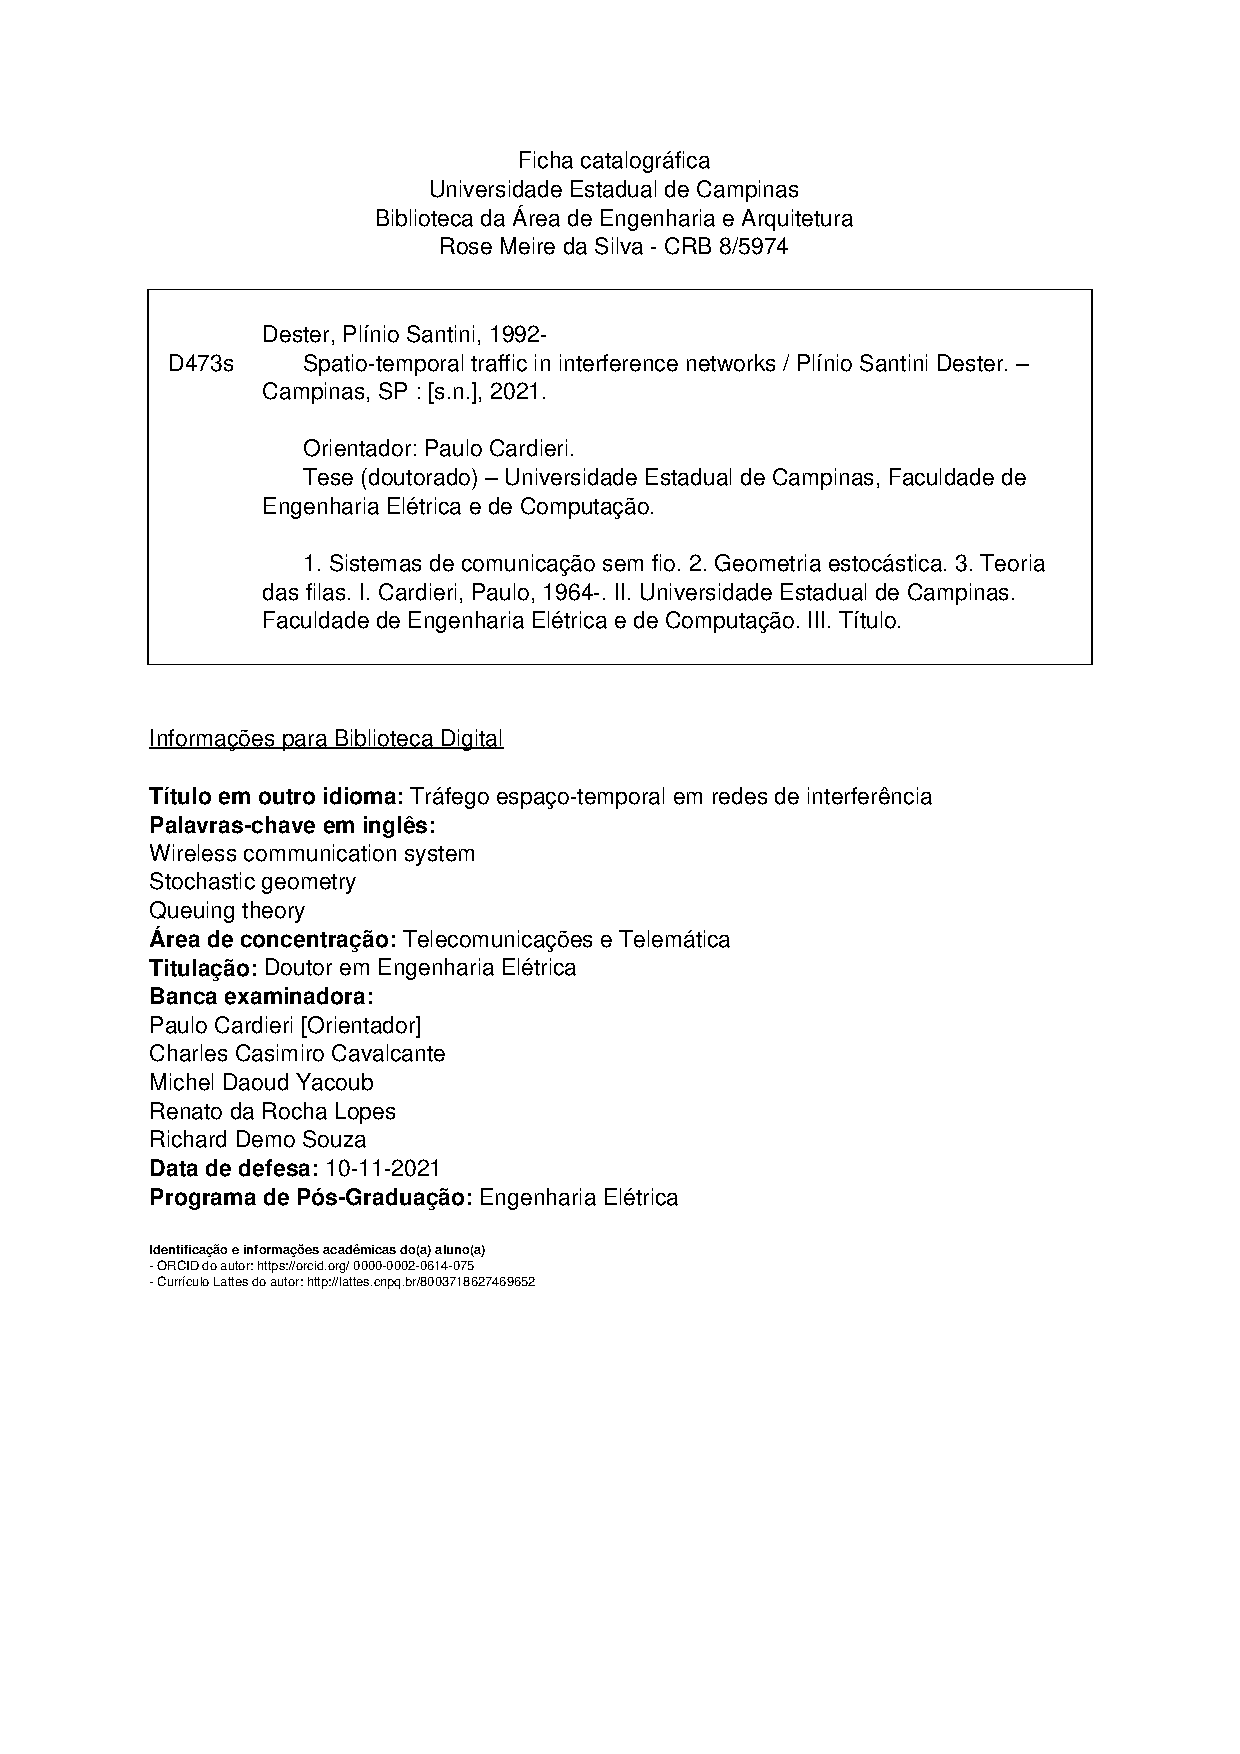
\includepdf{ficha-catalografica.pdf}
 \end{fichacatalografica}
% ---


% --- Inserir folha de aprova\c{c}\~{a}o ---

% Isto \'{e} um exemplo de Folha de aprova\c{c}\~{a}o, elemento obrigat\'{o}rio da NBR
% 14724/2011 (se\c{c}\~{a}o 4.2.1.3). Voc\^{e} pode utilizar este modelo at\'{e} a aprova\c{c}\~{a}o
% do trabalho. Ap\'{o}s isso, substitua todo o conte\'{u}do deste arquivo por uma
% imagem da p\'{a}gina assinada pela banca com o comando abaixo:

% --- Na vers\~{a}o final, exclua essas linhas e insira o \includepdf
% \newpage
% \vspace*{\fill}
% \begin{center}
    % \textsc{Inclua aqui a folha de assinaturas.}
% \end{center}
% \vspace*{\fill}
% \newpage
% --- --- ---
%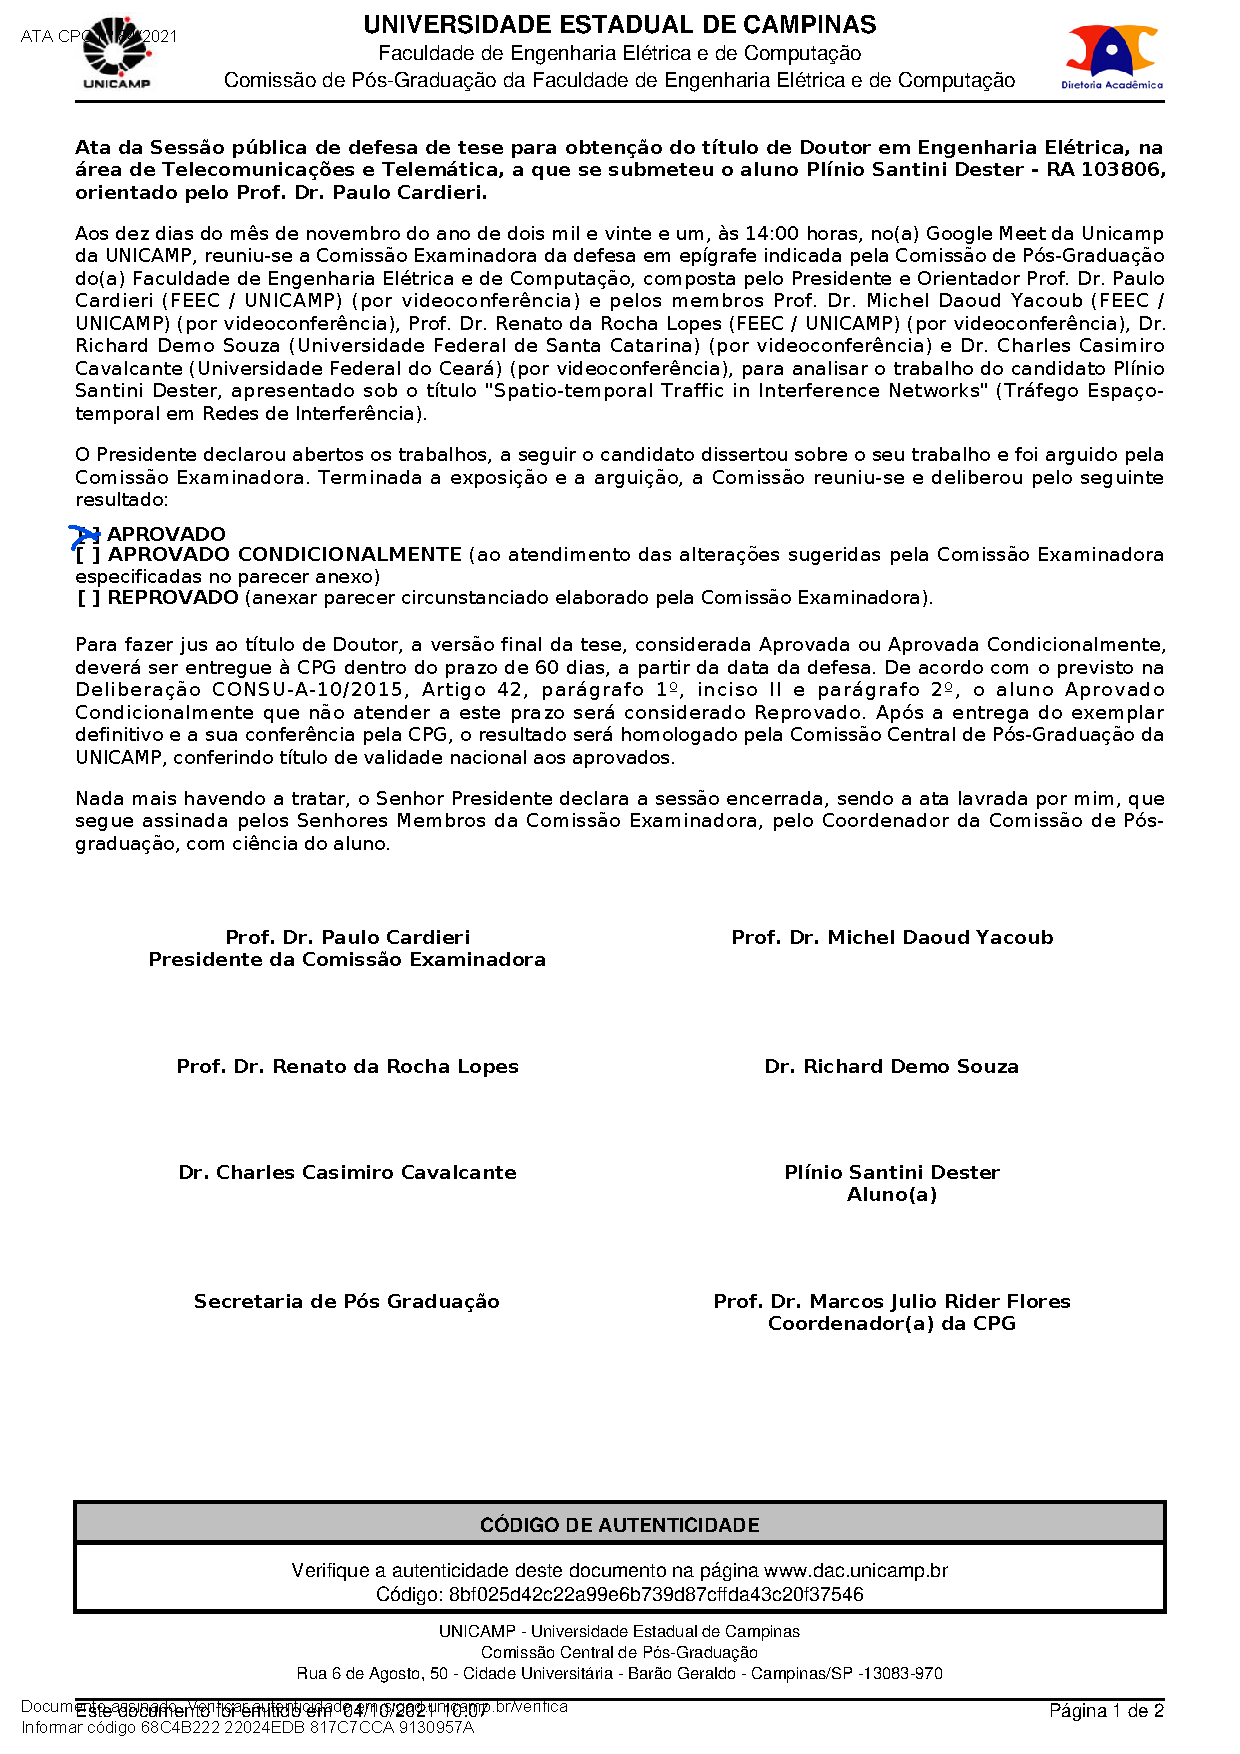
\includepdf[pagecommand={\thispagestyle{plain}}]{folha-assinaturas.pdf}	
% 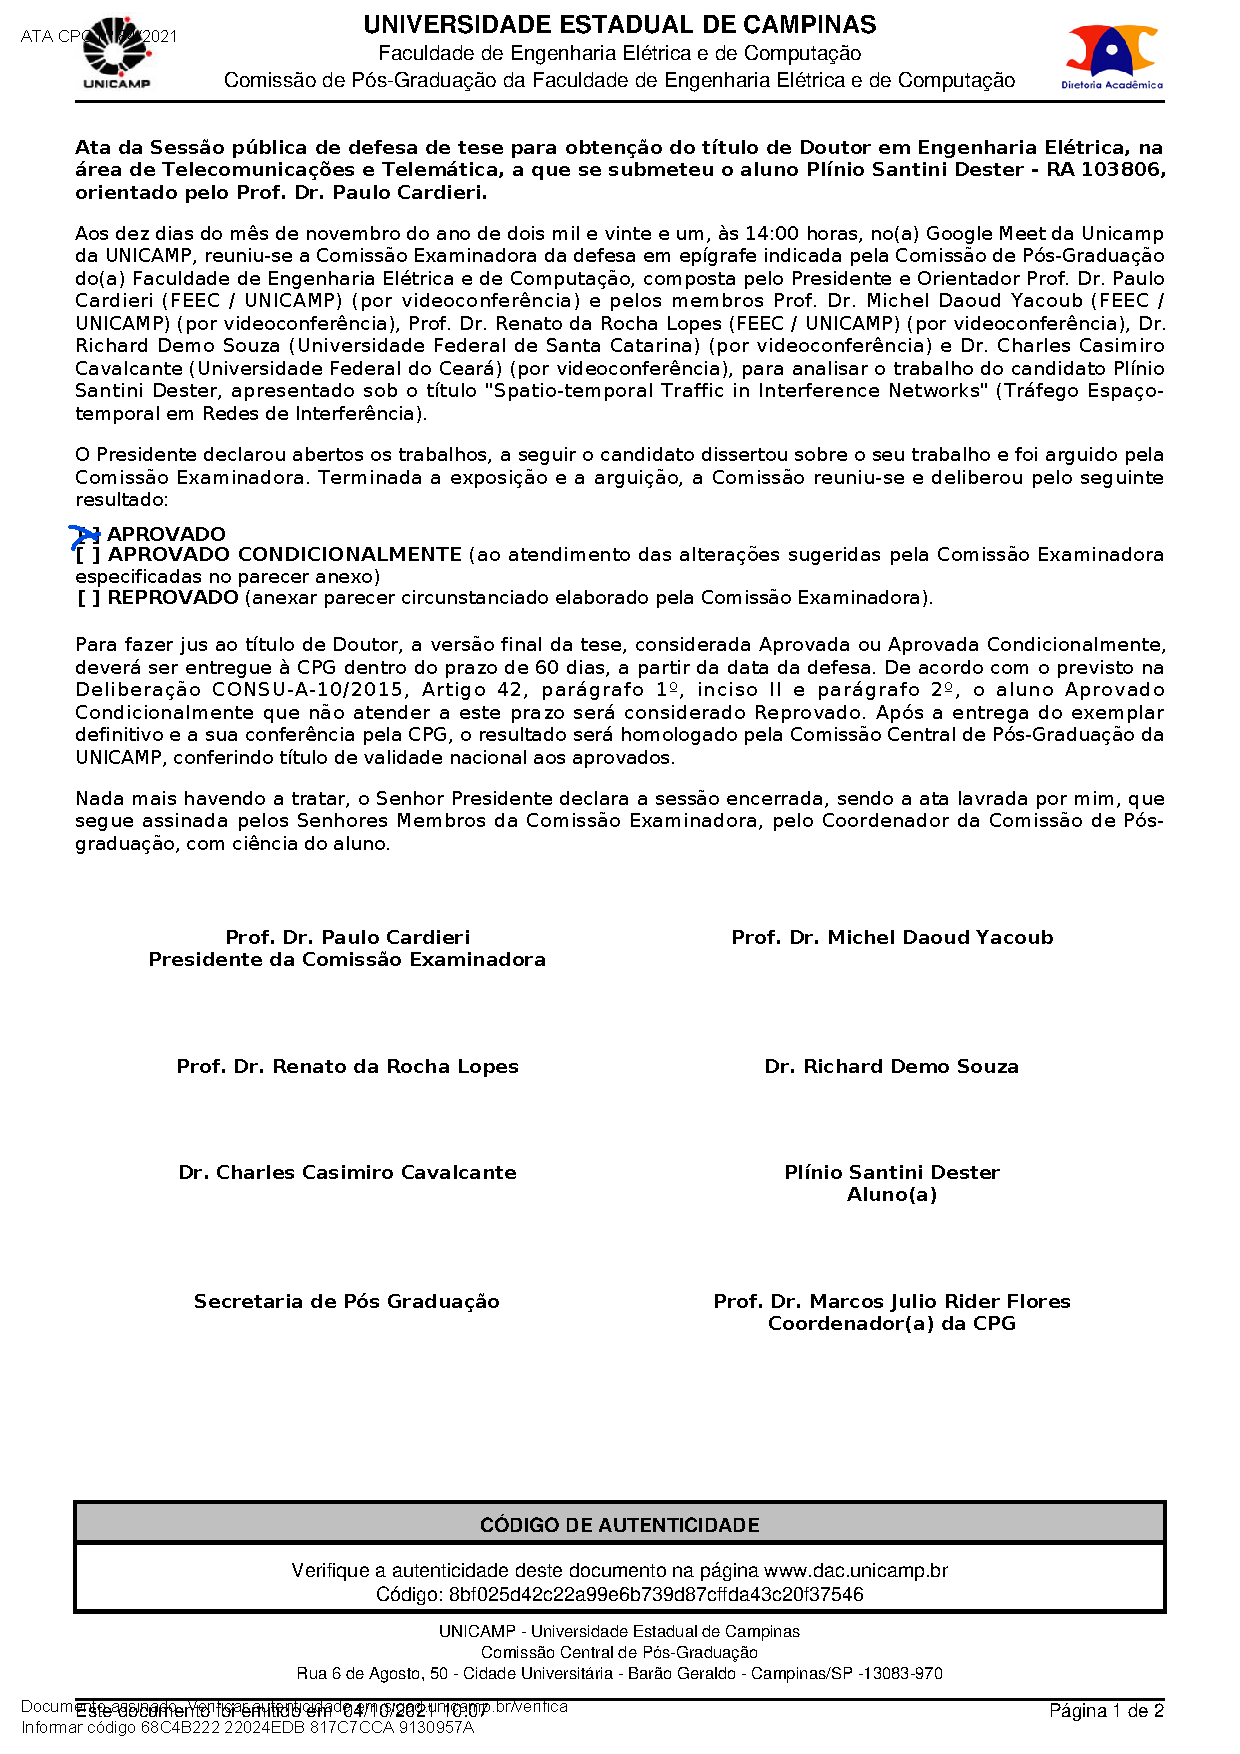
\includepdf[pages=1-3,pagecommand={\thispagestyle{plain}}]{folha-assinaturas.pdf}
% \cleardoublepage
% A Ata da defesa com as respectivas assinaturas dos membros encontra-se no SIGA/Sistema de Fluxo de Dissertação/Tese e na Secretaria do Programa da Unidade.

\begin{folhadeaprovacao}

\begin{center}
    {\Large\textsc{Comissão Julgadora -- Tese de Doutorado}}
    %\textsc{Inclua aqui a folha de assinaturas.}
\end{center}
\noindent
\begin{minipage}{\textwidth}\SingleSpacing
\textbf{Candidato:} Plínio Santini Dester \qquad \textbf{RA:} 103806

\textbf{Data de defesa:} 10 de novembro de 2021

\textbf{T\'{i}tulo da Tese:} ``Tráfego espaço--temporal em redes de interferência''
\vspace{2cm}

Prof. Dr. Paulo Cardieri (Presidente)

Prof. Dr. Charles Casimiro Cavalcante

Prof. Dr. Michel Daoud Yacoub

Prof. Dr. Renato da Rocha Lopes

Prof. Dr. Richard Demo Souza

\vspace{2cm}

\textit{A Ata de Defesa, com as respectivas assinaturas dos membros da Comiss\~{a}o Julgadora, encontra-se no SIGA (Sistema de Fluxo de Disserta\c{c}\~{a}o/Tese) e na Secretaria de P\'{o}s-Gradua\c{c}\~{a}o da Faculdade de Engenharia El\'{e}trica e de Computa\c{c}\~{a}o.}
\end{minipage}

\end{folhadeaprovacao}

% --- Dedicat\'{o}ria ---
\begin{dedicatoria}
    \vspace*{\fill}
    \centering
    \noindent
    \flushright{\large\textit{To my parents}}
    \vspace*{\fill}
\end{dedicatoria}
% ---

% --- Agradecimentos ---
\begin{center}
    \noindent{\Huge Acknowledgements}
\end{center}
I would like to express my gratitude to my parents Ivana and Mauricio who provided full support and were very comprehensive during the writing of this thesis.

I would like to thank my doctoral advisor Paulo Cardieri for his friendly, thoughtful, and flexible supervision, providing support whenever necessary.
%
I would also like to thank professor Pedro Henrique Juliano Nardelli who was practically a co-advisor for the published papers related to this thesis, and sent, from time to time, interesting and relevant articles to me.
%
I would also like to thank professor Rubem Toledo Bergamo, professor Francisco Helder Candido dos Santos Filho, and Rafael Augusto Pedriali for our collaborative works.
%
Thank you all for the opportunity to work alongside you!

In addition, I would like to thank professors:
%
Matheus Souza, for selecting me as PED for three semesters in different subjects and managing to not get tired of me (I think), it was a very pleasant and enriching experience;
%
Michel Yacoub, for the stimulating and friendly conversations about applied and non-applied mathematics;
%
Pedro Peres, for the patience and interest in hearing my mathematical ramblings, and for the exciting discussions about Borwein's sums/integrals and problems alike;
%
Renato Lopes, for the interesting conversations about probability theory;
%
João Bosco, for the end of class discussions about subtleties in some results from vector and complex calculus;
%
Marina Vachkovskaia, for including my ``challenge problems'' at the end of the lists of exercises, and making them worth bonus points for the solvers.
%
Thank you all, for the pleasant time spent together at UNICAMP.

I would like to acknowledge all the professors of \textit{École Polytechnique} and UNICAMP that contributed to my formation, specially the professors Philippe, Cândido, Clemente, Amorim, Violaro, Romis, Firer, Leo Pini, Alim, Mosna, Kleber, Gustavo, Max, Yaro, Pagan.

Further, I want to thank my friends and colleagues of the WissTek and surrounding labs for the pleasant times spent together, specifically Rafa, André, Tejerina, Diana, Byron, Rubem, Pedro, Fernando, Carlos, Francisco, Reginaldo, Yalena, Alessandro, Lucas, Cintia.

In addition, I would like to express my gratitude to Christine Fricker, which taught me much about mathematical writing; Christine checked every proof I wrote, provided feedback, and gave support during my internship at INRIA.
%
I would also like to include Danielle Tibi in this acknowledgement. Without Christine and Danielle it would not be possible to publish a result on the classical problem \textit{join the shortest queue}.

Further, I would like to thank my family, specially my aunt Iara. I also want to thank my friends Dani, Rique, Shiba, Tay, Marcos, Zé, Zé Cazarin, Gleison, Lionis, Gabes, Gaby, Carol, Caio, TioBacca, Allan, Gui, Nec, Luiz, Pudim, and Blanco that, through our Discord server \textit{Planilha is always an option}, kept me sane during the COVID-19 pandemic.

Finally, I would like to thank The São Paulo Research Foundation (FAPESP), which provided financial support to this research project through the grant 2017/21347-0.
\newpage

% \begin{agradecimentos}
%     I would like to express my gratitude to my parents Ivana and Mauricio who provided full support and were very comprehensive during the writing of this thesis.
    
%     I would like to thank my doctoral advisor Paulo Cardieri for his friendly, thoughtful, and flexible supervision, providing support whenever necessary.
%     %
%     I would also like to thank professor Pedro Henrique Juliano Nardelli who was practically a co-advisor for the published papers related to this thesis, and sent, from time to time, interesting and relevant articles to me.
%     %
%     I would also like to thank professor Rubem Toledo Bergamo, professor Francisco Helder Candido dos Santos Filho, and Rafael Augusto Pedriali for our collaborative works.
%     %
%     Thank you all for the opportunity to work alongside you!
    
%     In addition, I would like to thank professors:
%     %
%     Matheus Souza, for selecting me as PED for three semesters in different subjects and managing to not get tired of me (I think), it was a very pleasant and enriching experience;
%     %
%     Michel Yacoub, for the stimulating and friendly conversations about applied and non-applied mathematics;
%     %
%     Pedro Peres, for the patience and interest in hearing my mathematical ramblings, and for the exciting discussions about Borwein's sums/integrals and problems alike;
%     %
%     Renato Lopes, for the interesting conversations about probability theory;
%     %
%     João Bosco, for the end of class discussions about subtleties in some results from vector and complex calculus;
%     %
%     Marina Vachkovskaia, for including my ``challenge problems'' at the end of the lists of exercises, and making them worth bonus points for the solvers.
%     %
%     Thank you all, for the pleasant time spent together at UNICAMP.
    
%     I would like to acknowledge all the professors of \textit{École Polytechnique} and UNICAMP that contributed to my formation, specially the professors Philippe, Cândido, Clemente, Amorim, Violaro, Romis, Firer, Leo Pini, Alim, Mosna, Kleber, Gustavo, Max, Yaro, Pagan.
    
%     Further, I want to thank my friends and colleagues of the WissTek and surrounding labs for the pleasant times spent together, specifically Rafa, André, Tejerina, Diana, Byron, Rubem, Pedro, Fernando, Carlos, Francisco, Reginaldo, Yalena, Alessandro, Lucas, Cintia.
    
%     In addition, I would like to express my gratitude to Christine Fricker, which taught me much about mathematical writing; Christine checked every proof I wrote, provided feedback, and gave support during my internship at INRIA.
%     %
%     I would also like to include Danielle Tibi in this acknowledgement. Without Christine and Danielle it would not be possible to publish a result on the classical problem \textit{join the shortest queue}.
    
%     Further, I would like to thank my family, specially my aunt Iara. I also want to thank my friends Dani, Rique, Shiba, Tay, Marcos, Zé, Zé Cazarin, Gleison, Lionis, Gabes, Gaby, Carol, Caio, TioBacca, Allan, Gui, Nec, Luiz, Pudim, and Blanco that, through our Discord server \textit{Planilha is always an option}, kept me sane during the COVID-19 pandemic.
    
%     Finally, I would like to thank The São Paulo Research Foundation (FAPESP), which provided financial support to this research project through the grant 2017/21347-0.
% \end{agradecimentos}
% ---

% --- Ep\'{\i}grafe  ---
\begin{epigrafe}
    \vspace*{\fill}
    \chapterquote{%
    Le savant n'étudie pas la nature parce que cela est utile;\\
    il l'étudie parce qu'il y prend plaisir\\[.4ex]
    et il y prend plaisir parce qu'elle est belle.}%
    {-- Henri Poincaré, \textit{Science et méthode} (1908)}
    
    \chapterquote{%
    \small The scientist does not study nature because it is useful to do so.\\[.25ex]
    He studies it because he takes pleasure in it,\\[.1ex]
    and he takes pleasure in it because it is beautiful.}%
    {-- Henri Poincaré, \textit{Science and method} (1908)}
\end{epigrafe}
% ---

% --- RESUMOS (em portugu\^{e}s e ingl\^{e}s ---

\begin{resumo}
    In this thesis, we present a contribution to the area of wireless networks under random-access and limited by interference.
    %
    The first part of the manuscript introduces the necessary mathematical theory and, then, we state classical results on stochastic geometry and wireless networks.
    %
    The second part of the manuscript presents the network model used throughout the thesis.
    %
    Then, we present the contributions, which consist in fundamental studies related to understanding the limits and the behavior of this class of systems.
    %
    More specifically, we characterize, through some transmission success probability models, the distribution of the interference in a channel where packets are transmitted according to a Poisson process; 
    %
    we prove that the optimal random-access retransmission approach is to limit the maximum number of retransmissions to the smallest value that satisfies some constraint (such as throughput, traffic, or transmission/packet success probability) in a scenario where only the most recent packet matters;
    %
    we find closed form expressions to the stability region, transmission success probability and mean delay in a high-mobility Poisson network with $N$ different classes of users sharing the same channel;
    %
    using the aforementioned model we show that for $N=2$ classes of users, performing frequency bandwidth partition for one of the classes may improve the overall performance of the system;
    %
    we find an example in a commonly used Poisson network model for which the stationary distribution is not unique. Then, we provide sufficient conditions to guarantee unicity of the stationary in this Poisson network model assuming any path loss model and any distribution of link distances.
    \vspace{\onelineskip}

    \noindent\textbf{Keywords}: Wireless communication system, stochastic geometry, queueing theory.

    \vspace{\onelineskip}
    \vspace{\onelineskip}
    \newpage
    
    \begin{otherlanguage*}{brazil}
    \begin{center}{\ABNTEXchapterfont\huge Resumo}\end{center}
    Nesta tese, apresentamos contribuições para a área de sistemas de comunicação sem fio que utilizam acesso aleatório e são limitadas por interferência.
    %
    A primeira parte do texto introduz a teoria matemática necessária e, em seguida, enunciamos resultados clássicos da literatura de geometria estocástica e redes de comunicação sem fio.
    %
    A segunda parte do texto apresenta o modelo de rede que é utilizado no restante da tese.
    %
    Em seguida, apresentamos as contribuições, que constituem-se de estudos fundamentais relacionados à compreensão dos limites e do comportamento dessa classe de sistemas.
    %
    Mais especificamente, caracterizamos, através de alguns modelos de probabilidade de sucesso de transmissão, a distribuição da interferência em um canal onde os pacotes são transmitidos de acordo com um processo de Poisson.
    %
    Provamos que a abordagem de retransmissão de acesso aleatório ótima é limitar o número máximo de retransmissões ao menor valor que satisfaça alguma restrição (como taxa de transferência, tráfego ou probabilidade de sucesso de transmissão) em um cenário onde apenas o pacote mais recente importa;
    %
    encontramos expressões em forma fechada para a região de estabilidade, probabilidade de sucesso de transmissão e atraso médio em uma rede Poisson de alta mobilidade com $N$ classes diferentes de usuários compartilhando o mesmo canal;
    %
    usando o modelo anterior, mostramos que para $ N = 2 $ classes de usuários, realizar a partição da largura de banda de frequência para uma das classes pode melhorar o desempenho do sistema;
    %
    encontramos um exemplo em um modelo de rede de Poisson comumente utilizado para o qual a distribuição estacionária não é única. Em seguida, fornecemos condições suficientes para garantir a unicidade do estacionário neste modelo de rede de Poisson assumindo qualquer modelo de perda de percurso e qualquer distribuição de distâncias de enlace.
    \vspace{\onelineskip}

    \noindent\textbf{Palavras-chave}: Sistema de comunicação sem fio, geometria estocástica, teoria de filas.

    \end{otherlanguage*}
\end{resumo}
% ---


\begin{center}
    \noindent{\Huge List of Symbols}
\end{center}
\vspace{1cm}
% \vspace*{\fill}
% \noindent{\Huge List of Symbols}
% \vspace*{\fill}

\noindent
\begin{tabular}{l c l}
    $\N$        & \sep & Set of natural numbers: $\N = \{0,1,2,\dots\}$.\\
    $\Z$        & \sep & Set of integers.\\
    $\R$        & \sep & Set of real numbers.\\
    $\overline\R$   & \sep & The extended real line, i.e., $\overline\R = \R\cup\{-\infty,+\infty\}$.\\
    $\R^d$      & \sep & $d$-dimensional Euclidean space.\\
    $\C$        & \sep & Set of complex numbers.\\
    $\K^*$      & \sep & Set $\K$ without the null element: $\K^* = \K\backslash\{0\}$.\\
    $\K_+$      & \sep & Ordered set $\K$ without the negative elements: $\K_+ = \{x \in \K : x \ge 0\}$.\\
    $\P(\cdot)$        & \sep & Probability measure.\\
    $\delta_x(\cdot)$  & \sep & Dirac measure of set $\cdot$, equals $1$ if $x\in\cdot$ and $0$ otherwise.\\
    $\mu(\cdot)$       & \sep & Notation for a measure. If not specified, $\mu$ is the Lebesgue measure.\\
    $\Phi(\cdot)$      & \sep & Random measure or point process.\\
    $\E[\cdot]$ & \sep & Expected value operator.\\
    $|\cdot|$   & \sep & Modulus operator if $\cdot$ is a number, and cardinality if $\cdot$ is a set.\\
    $||\cdot||$ & \sep & Euclidean norm.\\
    $\ind_{A}(\cdot)$  & \sep & Indicator function of set $A$, equals $1$ if $\cdot\in A$ and $0$ otherwise.\\
    $\ind\!\left\{\cdot\right\}$  & \sep & Another form of the indicator function, equals $1$ if $\cdot$ is true and $0$ otherwise.\\
    $f\vert_A$      & \sep & Restriction of function $f$ by a smaller domain $A$.\\
    $\iu$       & \sep & Imaginary unit $\sqrt{-1}$.\\
    $\euler$    & \sep & Euler's number $2.71828\dots$\\
    $\pi$       & \sep & Pi number $3.14159\dots$\\
    $\equiv$    & \sep & Identical equality of functions.\\
    $\triangleq$ & \sep & Equal, by definition.\\
\end{tabular}
\cleardoublepage


% --- inserir o sumario ---
\renewcommand*{\cftchapterleader}{\hfill}
\settocdepth{section}
%
\pdfbookmark[0]{\contentsname}{toc}
\tableofcontents*
\clearpage
% \addtocontents{toc}{~\hfill\textbf{Page}\par}
% ---

% % --- inserir lista de ilustra\c{c}\~{o}es ---
% \pdfbookmark[0]{\listfigurename}{lof}
% \listoffigures*
% \cleardoublepage
% % ---

% % --- inserir lista de tabelas ---
% \pdfbookmark[0]{\listtablename}{lot}
% \listoftables*
% \cleardoublepage
% % ---

% % --- inserir lista de Acronimos e Abrevia\c{c}\~{o}es ---
% \renewcommand{\nomname}{Lista de Acr\^{o}nimos e Abrevia\c{c}\~{o}es}
% \pdfbookmark[0]{\nomname}{las}
% \printnomenclature
% \cleardoublepage
% % ---

% \begin{simbolos}
% \item[$ \Gamma $] Letra grega Gama
% \item[$ \Lambda $] Lambda
% \item[$ \zeta $] Letra grega minúscula zeta
% \item[$ \in $] Pertence
% \end{simbolos}

\pagenumbering{arabic}

\setlength{\abovedisplayskip}{6pt}
\setlength{\abovedisplayshortskip}{6pt}
\setlength{\belowdisplayskip}{6pt}
\setlength{\belowdisplayshortskip}{6pt}

% ---- ELEMENTOS TEXTUAIS ----
\textual

% ---- Chapters ----
\setcounter{page}{14}
\part{Preliminaries}

\chapter{Introduction}
\label{cap:P1_01} \thispagestyle{empty}
\def\printfig{1} % Cap. 1
\chapterquote{%
To see what is general in what is particular and\\
what is permanent in what is transitory is\\[.4ex]
the aim of scientific thought.}
{-- Alfred North Whitehead, \textit{An Introduction to Mathematics} (1911)}

Recent advances on wireless communications systems are pointing towards heterogeneous networks solutions with dense deployment of nodes \cite{hossain2014evolution}.
%
These wireless networks are expected to provide reliable connectivity to high-mobility devices, to users with millisecond delay constraints, and applications with gigabits per second of data rate requirements \cite{peng2015recent}.
%
This unceasing demand for higher throughput and lower latency leads to an ever-increasing traffic of packets.
%
Thus, the performance of wireless networks tends to be, each day more, limited by interference. % which depends on the spatial distribution of the interferers, the arrival process of packets, the queueing dynamics.

In this thesis, the studied telecommunication problem is the analysis of spatio-temporal traffic on wireless networks limited by interference.
%
In this first chapter, we provide a simple and introductory system model along with the approach for the analysis and the studied scenarios.
%
Note that a rigorous, general, and detailed model is provided in Chapter~\ref{cap:P2_00}.

\newpage
%-%-%-%-%-%-%-%-%-%-%-%-%-%-%-%-%-%
\section{The Problem}

In a wireless network, we have a set of transmitters and a set of receivers located across the space.
%
As time passes, for each transmitter is given packets that must be transmitted to a determined receiver as soon as possible.
%
Each packet is stored in a buffer and discarded upon successful reception by the corresponding receiver.

When a transmitter sends a packet, it interferes with other transmissions, and vice-versa. This aggregate interference is determined according to the transmit power of each transmitter, the transmission distance, and some random effects (e.g. fading).
%
Then, we determine whether a transmission was successful depending on the signal and the aggregate interference received by the receiver.

\textbf{What are the \textit{givens} of the problem?}%
\setlist{nolistsep}%
\begin{enumerate}[itemsep=1pt]
    \item The spatial position distribution of the transmitters and receivers.
    
    \item The arrival process of packets for each transmitter.
    
    \item The propagation model that affects the transmitted signals, e.g. path loss, fading.
    
    \item The network operation model or queueing system model, that describes the rules of packet buffering and transmitting, e.g. Aloha, CSMA.
    
    \item The transmission success probability model that decides whether a packet is successfully received based on the received signal and the received interference.
\end{enumerate}

\textbf{What do we want to \textit{know}?}%
\setlist{nolistsep}%
\begin{enumerate}[itemsep=1pt]
    \item Reliability metrics, i.e., metrics related to the transmission and packet success probabilities.

    \item Throughput metrics, i.e., metrics related to the number of successfully delivered packets, such as mean throughput, stability.
    
    \item Delay metrics, i.e., metrics related to the amount of time to deliver packets, such as mean delay, queue load, age-of-information.
\end{enumerate}

Regarding the \textit{givens}, we can relax them in some aspects.
%
For example, instead of working with a specific path loss model, we let the path loss model be an arbitrary function with some constraints.
%
When the problem is analytically tractable, usually there is little cost to let some well-chosen parameters (or even functions) be arbitrary.
%
Then, once we let a set of \textit{givens} arbitrary, we attain a better comprehension of the relationship between these \textit{givens} and the \textit{knowns} we are interested in.
%
We also obtain a generalization of the problem.

% In this sense, our approach is to study the tractable models used by the scientific community and let some of the ``givens'' be arbitrary.
% %
% More specifically, we choose the ``givens'' (e.g. arrival rate, access probability) for which we are interested in better understanding their relationship with the ``knowns'' (e.g. throughput, delay).

More specifically, the standard \textit{given} scenario of this thesis assumes a single class of users sharing the same frequency bandwidth and the following \textit{givens}:
\begin{enumerate}
    \item High-mobility Poisson network, i.e., the nodes' positions follow a Poisson point process.
    \item Packets arrive according to a Poisson (or Bernoulli) process.
    \item The signals are subjected to Rayleigh fading and power law path loss model.
    \item Packets are queued in infinite buffers, and transmitters access the channel according to a Poisson (or Bernoulli) process.
    \item Transmission success is decided by the capture model.
\end{enumerate}

% a high-mobility Poisson network under random-access, limited by interference, subject to Rayleigh fading and power law path loss model, packets are queued in infinite buffers, transmission success is decided by the capture model, and there is a single class of users sharing the same frequency bandwidth.
%
This standard model from the literature is easily (analytically) tractable, as it is shown in Section~\ref{sec:P1_03_02}.
%
For each scenario studied in this thesis, we list in Table~\ref{tab:givens} the \textit{givens} that we modified, flexibilized and generalized from the standard model, and the \textit{knowns} for which we established a connection.

\begin{table}[htb]
    \centering
    \begin{tabular}{c|l|l}
    \hline
    Location & Change on the \textit{givens}  & The \textit{knowns} \\
        \hline\hline
    Ch.~\ref{cap:P2_01} & transmission success models, no buffer
        & throughput, reliability \begin{tabular}[c]{@{}l@{}}~\\ ~ \end{tabular}\\\hline
    Ch.~\ref{cap:P2_02} & \begin{tabular}[c]{@{}l@{}}maximum number of retransmissions,\\ general transmission success model \end{tabular}
        & \begin{tabular}[c]{@{}l@{}}throughput, reliability,\\ delay, age-of-information\end{tabular}\\\hline
    Sec.~\ref{sec:high-mobility} & $N$ classes of users
        & \begin{tabular}[c]{@{}l@{}}stability, throughput, reliability,\\ delay, queue load\end{tabular} \\\hline
    Sec.~\ref{sec:bandwidth} & $2$ classes of users, bandwidth partition
        & \begin{tabular}[c]{@{}l@{}}stability, throughput, reliability,\\ delay, queue load\end{tabular}\\\hline
    Ch.~\ref{cap:P2_04} & \begin{tabular}[c]{@{}l@{}}static elements, general path loss model,\\ general distribution of link distances\end{tabular}
        & \begin{tabular}[c]{@{}l@{}}stability, queue load,\\
            stationary distribution\end{tabular}\\
    \hline
    \end{tabular}
    \caption{Variations on the \textit{givens} of the base model.}
    \label{tab:givens}
\end{table}

A thorough review of the literature models used in this thesis and their applications can be found in the tutorials \cite{haenggi2021stochastic, cardieri2010modeling}.

%-%-%-%-%-%-%-%-%-%-%-%-%-%-%-%-%-%
\section{Outline of the Thesis}

We assume the reader is familiar with probability theory, calculus, and optimization.
%
However, we do not assume familiarity with measure theory nor stochastic geometry. That is why we provide a succinct review on these subjects.
%
This knowledge is necessary for stating and understanding definitions and theorems from this thesis and from the well-celebrated books of stochastic geometry and wireless networks \cite{baccelli2010stochastic} and \cite{haenggi2012stochastic}.
%
Nevertheless, the reader that is not interested in mathematical details and proofs can skip some parts as indicated throughout the manuscript in notes highlighted with light-blue boxes.
%
Furthermore, for ease of reading, on the left side of every proof, there is a vertical line. Therefore, the proofs that do not interest the reader can be easily skipped.

In this manuscript, we differentiate \textit{lemmas}, \textit{theorems}, and \textit{propositions} in the following manner.
%
We let the short and mathematical results that are used to prove other statements be the \textit{lemmas}.
%
For the results which are related to the physical problem, yet they have a mathematical basis in the sense that their existence is independent of the physical problem, those we call \textit{theorems}.
%
Finally, the results which are strongly related to the physical problem and alone do not have significance, those we call \textit{propositions}.

Throughout the thesis, we also have the \textit{remarks} and the \textit{notes}, which are highlighted in gray and light-blue boxes, respectively.
%
Their purpose is to comment on aforementioned results.
%
We reserve the more contextualized and formal comments to the \textit{remarks}, and the more digressive and informal comments to the \textit{notes}.

% We decided to include several definitions, because when we say that the system model is over a ``stationary and ergodic Poisson network'' the reader is able to check what exactly that means.

% \begin{itemize}
%     \item Mathematical optimization.
%     %
%     This knowledge is necessary for stating and understanding definitions and theorems from stochastic geometry presented on the well celebrated books \cite{baccelli2010stochastic} and \cite{haenggi2012stochastic}.
    
%     \item (alternatively) In this thesis we need measure theory (applied to integration and probability) to present and prove some results. Since this is not a common subject in the engineering curriculum, we provide a succinct introduction of this topic in Chapter~\ref{cap:P1_02} focusing on the results we need.
    
%     \item The thesis is readable without measure theory, except for Chapter~\ref{cap:P1_03} and some proofs.
    
%     \item We tried to be mathematically rigorous because we have general results and it is not possible to simulate every representative choice of model to guarantee them;
    
%     \item General results in the sense that they are valid for arbitrary functions that represent, e.g, the path loss, the success transmission model, the link distance distribution.
    
%     \item We are following the formalism adopted in the well celebrated books in the area of stochastic geometry applied to wireless networks \cite{baccelli2010stochastic}, \cite{haenggi2012stochastic}.
% \end{itemize}

This thesis is organized in nine chapters and two appendices.
%
This first chapter presents, in an intuitive and general manner, the main problem and the approach adopted to study it.
%
The other chapters are summarized below.

\begin{description}
    \item[Chapter~2:] We present the notations and definitions used throughout the manuscript. We also provide a succinct review of measure theory applied to integration and probability. They are necessary to understand stochastic geometry and several proofs of this thesis.
    
    \item[Chapter~3:] In this chapter, we present the theory of point processes and random measures. Then, we present some known and extensively used results of stochastic geometry applied to wireless networks.
    
    \item[Chapter~4:] This is the first chapter with contributions.
    We present a general system model for a wireless network and some definitions, which are used until the end of the thesis.
    
    \item[Chapter~5:] We consider a Poisson process to model packet transmissions and characterize the distribution of the interference in this model.
    
    \item[Chapter~6:] This chapter includes retransmission and analyzes the impact of this strategy in the throughput and delay.
    
    \item[Chapter~7:] Here we include the spatial positions of the nodes in the analysis. We also model the buffers of the transmitters as queues and study their stability.
    
    \item[Chapter~8:] In this chapter we introduce static elements. More precisely, the link distances between transmitters and receivers are fixed across time. This consists of a challenging class of problems because static elements hinder tractability.
    
    \item[Chapter~9:] We conclude the thesis listing the main contributions and prospects for future research.
    
    \item[Appendix~A:] Some definitions and results of real analysis used in the thesis.
    
    \item[Appendix~B:] A brief review of queueing theory (delay, stability).
\end{description}

%-%-%-%-%-%-%-%-%-%-%-%-%-%-%-%-%-%
\section{Author's Publications}

This thesis is based on three published international journal papers \cite{dester2018,dester2021unique, dester2021retrans}, and one submitted paper \cite{dester2021part}.
%
Besides, the author has three published international journal papers \cite{dester2017stationary, francisco2020, bergamo2021} and two conference papers \cite{dester2018mtc, helder2019lora} that are not covered by this thesis.


\chapter{Mathematical Preliminaries}
\label{cap:P1_02} \thispagestyle{empty}
\def\printfig{1} % Cap. 2
\chapterquote{%
Mathematics is the art of giving the same name\\[0.4ex] to different things.}%
{-- Henri Poincar\'e, \textit{Science et méthode} (1908)}

% \chapterquote{%
% Every definition implies an axiom, since it asserts the existence of the object defined. The definition then will not be justified, from the purely logical point of view, until we have proved that it involves no contradiction either in its terms or with the truths previously admitted.}%
% {Henri Poincar\'e, \textit{Science et méthode (1908)}}

In this chapter, we present some notations, mathematical concepts, definitions, and results that are fundamental to the development of the thesis.
%
For further details and proofs, please refer to the classic book:
%
\begin{itemize}
    % \item \cite{rudin1976principles} and \cite{rudin1987real} for Calculus, Real Analysis and Complex Analysis.
    \item \textit{Probability and Measure} \cite{billingsley1986probability}.
\end{itemize}

We opted to include this chapter for self-containment purposes regarding definitions and theorems frequently used in the manuscript.
%
Further, we comment on the reasons behind some of them, and on problems the lack of such formalism could entail on the applications.

This chapter can also be used as a succinct preparation to read the well-celebrated book \textit{Stochastic Geometry and Wireless Networks} \cite{baccelli2010stochastic} which requires some knowledge on measure theory and it is one of the books we used as a basis to write Chapter~\ref{cap:P1_03}.

\begin{note}
    The reader that is not interested in mathematical details can skip to Chapter~\ref{cap:P1_03} and consult this chapter as needed.
\end{note}

\newpage

% % % % % % % % % % % % % % % % % % % % % % % % % % % 
% % % % % % % % % % % % % % % % % % % % % % % % % % % 
\section{Notations and Definitions}

% % % % % % % % % % % % % % % % % % 
\subsection{Asymptotic notation}

The asymptotic notation, also known as Bachmann--Landau notation or big O notation, is very useful to express complicated terms of a mathematical expression that are dominated by other terms and are not relevant to the analysis.
%
The definition follows.

\begin{definition}[\textbf{Landau notation}] \label{def:landau}
    Let $f$ and $g$ be functions from $\R$ into $\R$ and $a\in\R\cup\{\infty,-\infty\}$.
    %
    We write that $f(x) = \cal{O}(g(x))$ as $x$ tends to $a$ if and only if
    \begin{align*}
        \limsup_{x\to a} \left| \frac{f(x)}{g(x)} \right| < \infty.
    \end{align*}
    
    % Further, we write $f(x) = o(g(x))$ as $x$ tends to $a$ if and only if
    % \begin{align*}
    %     \lim_{x\to a} \left| \frac{f(x)}{g(x)} \right| = 0 .
    % \end{align*}
\end{definition}

This notation is somewhat misleading because despite the use of the equality symbol, it does not possess the reflexive nor the transitive property, e.g.,
%
if $f(x)=\cal{O}(1/x)$ and $g(x)=\cal{O}(1/x)$ as $x\to\infty$, we cannot say that $f(x) = g(x)$.
%
Also, we know that $\cal{O}(x^3) = \cal{O}(x^2)$ as $x\to0$, however we cannot say that $\cal{O}(x^2) = \cal{O}(x^3)$ as $x\to0$.
%
A set notation would be more consistent in this sense. For example, $\cal{O}(x^3) \subset \cal{O}(x^2)$ as $x\to0$ would mean that the class of functions bounded by $x^2$ is a subset of the class of functions bounded by $x^3$ as $x$ tends to $0$.
%
However, we shall stick with the usual notation to avoid confusion and for convenience.

\begin{example} Using Landau notation, the Taylor expansion of $\tan(\cdot)$ around $0$ is
    \begin{align*} 
        \tan(x) = x + \frac{x^3}{3} + \frac{2x^5}{15} + \cal{O}(x^7)\qquad \text{as $x$ tends to $0$}.
    \end{align*}
\end{example}



% % % % % % % % % % % % % % % % % % 
\subsection{Closed form expression}
What is considered a closed form expression varies from author to author and depends on context.
%
A thorough analysis of this topic can be found in \cite{borwein2013closed}, where the authors present several definitions of closed form expressions and their importance for science.
%
All in all, to be clear what we mean by closed form expression in this manuscript, we provide the definition below.
\begin{definition}[\textbf{Closed form}] \label{def:closed_form}
    A mathematical expression is in \textit{closed form} if and only if it can be expressed as a finite combination of constants, field operations\footnote{Addition, subtraction, multiplication, and division.}, and linear, exponential, and logarithmic functions.
    
    When we say \textit{closed form} in terms of $\cdot$\,, we include $\cdot$ in the list of allowed functions.
\end{definition}

Note that the above definition includes trigonometric and inverse trigonometric functions. For example, let $x\in\R$ or $x\in\C$,
\begin{align*}
    \sin(x) = \frac{\euler^{\iu x}-\euler^{-\iu x}}{2\iu}, \qquad \arctan(x) = \frac{1}{2\iu} \ln\!\left(\frac{\iu-x}{\iu+x}\right).
\end{align*}

Further, this definition agrees with the well-known Abel–Ruffini theorem, which states that there is no \textit{closed form} solution for general polynomial equations of degree five or higher.
%
Indeed, this is not true anymore if we consider, for example, \textit{closed form} expressions in terms of hypergeometric functions \cite{chow1999closed}.

\subsection{Discrete}

We all know what ``discrete'' means. However, a formal definition is not immediate. If we say that a set is discrete if it is \textit{countable}\footnote{A set is \textit{countable} if there exists an injective function from the set to the natural numbers $\N$.}, then $\Q$ is a discrete set. However, we do not want to include $\Q$ in this category, because this set is dense in $\R$, i.e., the set of limit points of $\Q$ results in $\R$.
% %
Thus, a more refined definition is necessary. Assuming a metric space (Definition~\ref{def:metric_space}) we can define a discrete set as follows.

\begin{definition} \label{def:discrete}
    A set $A$ is discrete if every point in $A$ is an isolated point\footnote{A point is isolated if there exists a neighborhood (Definition~\ref{def:neighborhood}) that only contains the point.}.
\end{definition}

This definition is enough for our purposes. However, some questions arise.
%
The set $$A = \left\{\frac{1}{n} : n\in\N^*\right\} = \left\{1,\frac{1}{2},\frac{1}{3},\frac{1}{4},\dots\right\}$$ is discrete because for any given point of this set we can take a sufficiently small open interval (neighborhood) such that it contains only the given point.
%
On the other hand, take the set $$B = A \cup \{0\} = \left\{0,1,\frac{1}{2},\frac{1}{3},\frac{1}{4},\dots\right\}.$$
%
Note that we cannot take an open interval around $0$ such that it only contains $0$. Thus, this set is not discrete according to our definition.

This is strange, since $A$ is discrete and very similar to $B$.
%
Perhaps we should include in the definition that a set is discrete if every point in the set is isolated, except for a finite number of points in the set. Then, $A$ and $B$ would be discrete.

All in all, this discussion is out of the scope of this thesis.
%
Nevertheless, we noticed an apparent lack of this fundamental definition in the literature related to this thesis. Although not serious it is disquieting. Indeed, we ``borrowed'' Definition~\ref{def:discrete} from topology.

\subsection{Probability distributions}

In Table~\ref{tab:distributions}, we present the probability distributions most used throughout the thesis.
%
\def\arraystretch{1.8}
\begin{table}[H]
    \centering
    \begin{tabular}{c|c|c|c|c}
    \hline
        Distribution  & symbol & density $f_X$ & support $X(\Omega)$ & parameters\\ \hline\hline
        Bernoulli & $\mathscr{B}(p)$ & {\footnotesize$p\,k+(1-p)(1-k)$}  & $k\in\{0,1\}$ & $p\in[0,1]$\\
        Binomial & $\mathscr{B}_n(p)$ & \footnotesize$\displaystyle\binom{n}{k} p^k(1-p)^{n-k}$ & $k\in\{0,1,\dots,n\}$ & $n\in\N^*, p\in[0,1]$\\
        Geometrical & $\mathscr{G}(p)$ & \footnotesize$(1-p)^k\,p$ & $k\in\N$ & $p\in[0,1]$\\
        Exponential & $\mathscr{E}(\lambda)$ & \footnotesize$\lambda \,\euler^{-\lambda x}$ & $x\in\R_+$ & $\lambda\in\R_+^*$\\
        Erlang & $\mathscr{E}_n(\lambda)$ & \footnotesize$\displaystyle\frac{\lambda^n x^{n-1}}{(n-1)!} \,\euler^{-\lambda x}$ & $x\in\R_+$ & $n\in\N^*,\lambda\in\R_+^*$\\
        Poisson & $\mathscr{P}(\lambda)$ & \footnotesize$\displaystyle\frac{\lambda^k}{k!} \,\euler^{-\lambda}$ & $k \in \N$ & $\lambda\in\R_+^*$\\
    \hline
    \end{tabular}
    \caption{Considering the probability space $(\Omega,\cal F, \P)$ and a random variable $X$.}
    \label{tab:distributions}
\end{table} \vspace{-3mm}
\def\arraystretch{1}
%
Then, if a random variable $X$ follows an exponential distribution of parameter $\beta>0$, we denote simply as $X\sim\mathscr{E}(\beta)$.
%
Note that $\mathscr{B}_1$ is equivalent to $\mathscr{B}$ and $\mathscr{E}_1$ to $\mathscr{E}$.
%
This is related to the fact that the sum of $n$ iid\footnote{A sequence of random variables is iid if the random variables are independent and identically distributed.} Bernoulli (Exponential) distributed random variables follow a Binomial (Erlang) distribution of parameter $n$.

\begin{note}[\textbf{Poisson process}]
    An interesting fact related to the distributions of Table~\ref{tab:distributions} is that the Poisson process, that models a collection of points randomly positioned in the real line $\R$, somehow contains all these distributions.
    
    First, the Poisson distribution. We define the Poisson process of density $\lambda>0$ through a collection of random variables $\{N([a,b])\}_{a<b}$, where $N([a,b])\sim\mathscr{P}(\lambda(b-a))$ gives the number of points for every interval $[a,b] \subset \R$.
    %
    For the Exponential distribution, the length of the interval between two consecutive points of the Poisson process follows $\mathscr{E}(\lambda)$.
    %
    Then, the Erlang distribution follows immediately by taking the length of the interval between the first and the last of $n+1$ consecutive points. This length follows $\mathscr{E}_n(\lambda)$.
    %
    For the Binomial distribution, let $a<b<c$, i.e., $[a,b]\subset[a,c]$. Then, $N([a,b])\mid \{N([a,c])=n\} \sim \mathscr{B}_n((b-a)/(c-a)).$
    The Bernoulli distribution follows immediately by taking $n=1$.
    %
    Finally, the Geometrical distribution appears as
    $\min\{k\in\N : N([k,k+1)) > 0\} \sim \mathscr{G}(1-\euler^{-\lambda}).$
\end{note}

% % % % % % % % % % % % % % % % % % % % % % % % % % % 
% % % % % % % % % % % % % % % % % % % % % % % % % % % 
\section{Sets and Measurability}

%  \subsection{The \texorpdfstring{$\sigma$}{σ}-algebra}

While the intricacies of measure theory are out of the scope of this work, we still need to clarify what ``measurable'' means.
%
For that, we need to introduce some definitions. The following one imposes a constraint on the subsets we can choose from a given set.

% A set is \textit{countable} if there exists an injective function from the set to the natural numbers $\N$.

\begin{definition}[\textbf{$\sigma$-algebra}]
    Let $A$ be a set.
    %
    A $\sigma$-algebra $\cal{A}$ over set $A$ is an algebra of sets which is closed under \textit{countable}\footnote{%A set is \textit{countable} if there exists an injective function from this set to the natural numbers. 
    Here \textit{countable} unions means the index set is \textit{countable}.} unions, i.e., $\cal{A}$ satisfies the following properties.
    %
    \setlist{nolistsep}
    \begin{enumerate}[label=(\alph*), noitemsep]
        \item $\varnothing\in\cal A$.
        \item If $E\in\cal A$, then $E^c\triangleq\{a\in A\mid a\notin E\}\in\cal A$.
        \item If $E_i\in\cal A$ for every $i\in\N$, then $\displaystyle\bigcup_{i\in\N} E_i\in\cal A$.
    \end{enumerate}
    %
    The pair $(A,\cal{A})$ is called a \textit{measurable space}.
\end{definition}

In general terms, a $\sigma$-algebra consists of a collection of desirable subsets of $A$, e.g. in probability theory all the events of a sample space $\Omega$ must form a $\sigma$-algebra.
%
Note that we only require a \textit{countable} union of subsets to belong to the $\sigma$-algebra. An \textit{uncountable} union would allow problematic sets, e.g. the Vitali set \cite{vitali1905sul}, which is a subset of $\R$ that we cannot define a useful form to ``measure'' its length. A \textit{measure} is defined as follows.

\begin{definition}[\textbf{Measure}]
    Let $(A,\cal{A})$ be a \textit{measurable space}.
    %
    Let $\mu: \cal{A}\longrightarrow \R \cup \{\infty\}$. Then $\mu$ is called a \textit{measure} on $\cal{A}$ if and only if $\mu$ has the property of countable additivity
    \begin{align*}
        \mu\!\left(\bigcup_{n\in\N} E_n \right) = \sum_{n\in\N} \mu(E_n)
    \end{align*}
    for all pairwise disjoint $E_n \in\cal{A}$, and satisfies $\mu(\varnothing) = 0$ and $\mu(E) \ge 0$ for all $E \in \cal{A}$.\\
    %
    The triple $(A,\cal{A},\mu)$ is called a \textit{measure space}, or \textit{probability space} when $\mu(A)=1$.
\end{definition}

Three fundamental measures used in this work are the Lebesgue measure, the counting measure, and the probability measure.
%
The Lebesgue measure consists of the standard way to measure subsets of the $\R^d$ and coincides with length for $\R$, area for $\R^2$, and volume for $\R^3$.
%
The counting measure is the ``natural'' measure of \textit{countable} sets; it gives the number of elements of a subset of a set and coincides with its cardinality if the subset is finite.
%
The probability measure is the measure associated with the \textit{measure space} $(\Omega,\cal{F},\P)$, which we call the \textit{probability space} and serves to model a random process or ``experiment''. The set $\Omega$ is the sample space and contains all possible outcomes, the $\sigma$-algebra $\cal{F}$ is the event space and contains the measurable subsets of $\Omega$, and we require that the measure of the entire sample space is equal to one, i.e., $\P(\Omega) = 1$.

Another problematic implication of not using \textit{measurable} sets is known as the Banach-Tarski paradox \cite{banach1924decomposition}, which maps a finite decomposition of a solid ball of the $\R^3$ into two identical disjoint balls using only translations and rotations.

Thus, from now on, we shall only use \textit{measurable} sets to avoid running into problems such as an event having a probability equal to $2$.
%
The standard choice for a ``well-behaved'' $\sigma$-algebra is the Borel $\sigma$-algebra over a set $A$ and it is denoted as $\cal{B}(A)$, which is the smallest $\sigma$-algebra that contains all open subsets of $A$.
%
This is enough for our applications, thus whenever the $\sigma$-algebra is not specified, we are using the Borel $\sigma$-algebra.

It is worth noting that, in a \textit{probability space} $(\Omega,\cal{F},\P)$ where the set $\Omega$ is \textit{countable}, we can choose all the partitions of $\Omega$ as the $\sigma$-algebra.
%
Problems with \textit{non-measurable} subsets arise when $\Omega$ is not \textit{countable}, e.g. $\Omega = \R$, for which we must carefully choose the $\sigma$-algebra.

Another care we must take emerges when mapping a set into another. The idea is to guarantee that the preimage of any measurable set is measurable.
%
The functions that satisfy this property are called \textit{measurable functions} and this is essential to integrate a function or to measure the probability of a random variable assuming values in a given set.
%
The definition follows.

\begin{definition}[\textbf{Measurable function}]
    Let $(A,\cal{A})$ and $(A',\cal{A}')$ be \textit{measurable spaces}.
    %
    Then a function ${f: A\longrightarrow A'}$ is said to be \textit{measurable} if and only if for all $E \in \cal{A}'$
    \begin{align*} 
        f^{-1}(E) \triangleq \{ x\in A \mid f(x)\in E \} \in \cal{A}.
    \end{align*}
\end{definition}
%

% % % % % % % % % % % % % % % % % % % % % % % % % % % 
% % % % % % % % % % % % % % % % % % % % % % % % % % % 
\section{Integration with Respect to a Measure}

The purpose of this section is to present some definitions and results from the theory of integration with respect to a \textit{measure}.
%
Let us start with the definition of the integral operator.

\begin{definition}
    Let $(A,\cal A, \mu)$ be a \textit{measure space} and $f:A\longrightarrow \overline\R$ be a non-negative \textit{measurable} function.
    %
    We define the integral of $f$ on $A$ with respect to the measure $\mu$ as
    \begin{align*}
        \int f \, \d \mu \triangleq \sup_{\substack{\{A_i\}_i^n \in \cal A,\\ n \in \N}} \left\{ \sum_i^n \left( \inf_{x\in A_i} f(x) \right) \mu(A_i) ~\middle\vert~ \bigcup_i^n A_i = A\right\}
    \end{align*}
    with the convention $0\cdot\infty = 0$.
\end{definition}

Note that the above definition is only for non-negative functions. However, this is easily extended for general $f$ by separating the function into positive and negative parts, integrating separately and, then, subtracting the results.
%
It is important to note that $\infty - \infty$ is undefined.

Other notations we shall use for the integral of $f$ is
\begin{align*}
    \int f \, \d \mu = \int f(x) \, \d\mu(x) = \int f(x) \, \mu(\d x).
\end{align*}

We say a function $f$ is integrable if and only if
\begin{align*}
    \int |f| \,\d\mu < \infty.
\end{align*}

In case $\mu$ is the Lebesgue measure on $\R^d$, we use the classical notation
\begin{align*}
    \int f \,\d\mu = \int_{\R^d} f(x)\,\d x.
\end{align*}

Now we present some fundamental theorems that give sufficient conditions to interchange the limit operator with the integral operator.
%
These theorems are one of the main motivations to use the Lebesgue integral (in case $\mu$ is the Lebesgue measure) over the Riemann integral.
%
Nevertheless, note that the following theorems are valid for general measures.

\begin{theorem}[\textbf{Monotone convergence theorem}]
    Let $(A,\cal A, \mu)$ be a \textit{measure space}. For every non-decreasing sequence\footnote{A non-decreasing sequence of functions means that $f_{n+1}(x)\ge f_n(x)$ for all $x$.} $\{f_n\}_{n\in\N}$ of $\overline\R_+$-valued \textit{measurable} functions we have
    \begin{align*}
        \lim_{n\to\infty} \int f_n \,\d\mu = \int \lim_{n\to\infty} f_n \,\d\mu.
    \end{align*}
\end{theorem}

\begin{theorem}[\textbf{Fatou's lemma}]
    Let $(A,\cal A, \mu)$ be a \textit{measure space}. For every sequence $\{f_n\}_{n\in\N}$ of $\overline\R_+$-valued \textit{measurable} functions we have
    \begin{align*}
        \liminf_{n\to\infty} \int f_n \,\d\mu = \int \liminf_{n\to\infty} f_n \,\d\mu.
    \end{align*}
\end{theorem}

\begin{theorem}[\textbf{Lebesgue's dominated convergence theorem}]
    Let $(A,\cal A, \mu)$ be a \textit{measure space}. Let $\{f_n\}_{n\in\N}$ be a sequence of $\overline{\R}$-valued measurable functions such that $f_n \to f$ \textit{almost everywhere}\footnote{A property holds \textit{almost everywhere} if it is true for all points except for a subset of measure $0$.} as $n\to\infty$.
    %
    If there exists an integrable function $g$ such that $|f_n|\le g$ \textit{almost everywhere} and for every $n\in\N$, then
    \begin{align*}
        \lim_{n\to\infty} \int f_n \,\d\mu = \int f \,\d\mu.
    \end{align*}
\end{theorem}

\begin{theorem}[\textbf{Leibniz integral rule}] \label{th:leibniz}
    Let $(A,\cal A, \mu)$ be a \textit{measure space} and $(T, \cal T)$ a \textit{measurable space}.
    %
    Let $f:A\times T \longrightarrow \R$ be a measurable function that has a derivative $f'$ in the open set $T\subset\R$.
    %
    If there exists an integrable function $g$ such that $|f'(x,t)|\le g(x)$ for \textit{almost} every $x\in A$ and for every $t\in T$, then
    \begin{align*}
        \frac{\d}{\d t} \int f(x,t)\,\d\mu(x) = \int \frac{\d}{\d t} f(x,t) \,\d\mu(x), \qquad t \in T.
    \end{align*}
\end{theorem}

All the above theorems hold even if we integrate in a subset $B\in\cal A$ of $A$. That is easy to see with the function $\ind_B \cdot f$.
%
Indeed, we define the integral of $f$ over set $B$ as
\begin{align*}
    \int_B f\,\d\mu \triangleq \int \ind_B(x) f(x) \,\d\mu(x).
\end{align*}

Furthermore, these results are also valid for infinite series, because we can take the \textit{measure space} $(\Z,\cal B(\Z), \mu)$ with $\mu$ being the counting measure. In such case we have
\begin{align*}
    \int f\,\d\mu = \sum_{x\in\Z} f(x).
\end{align*}

The following theorem guarantees the change of variable method in integration.

\begin{theorem}[\textbf{Change of variable}]
    Let $(A,\cal A, \mu)$ and $(A', \cal A', \nu)$ be \textit{measure spaces}.
    %
    Let the mapping $\varphi:A\longrightarrow A'$ be a \textit{measurable} function and $\nu = \mu\varphi^{-1}$, which is a measure that satisfies \vspace{-5mm}
    \begin{align*}
        \mu\varphi^{-1}(B') = \mu(\varphi^{-1}(B')) \quad \forall B'\in\cal{A}'.
    \end{align*}
    
    A \textit{measurable} function $f:A'\longrightarrow\R$ is integrable with respect to $\mu\varphi^{-1}$ if and only if $f\circ\varphi$ is integrable with respect to $\mu$, in which case
    \begin{align*}
        \int_{\varphi^{-1}(B')} f(\varphi(x))\,\d\mu(x) = \int_{B'} f(x') \,\d\mu\varphi^{-1}(x'), \qquad B'\in\cal{A}'.
    \end{align*}
\end{theorem}

For the Lebesgue measure, we have a more explicit method as described below.
\begin{theorem}[\textbf{Change of variable on $\R^d$}]
    Let $\varphi$ be a continuously differentiable %\footnote{Continuously differentiable means the derivative exists and is continuous.}
    injective map from the open set $U\subset\R^d$ onto $V\subset\R^d$.
    %
    If $f$ is a nonnegative measurable function, then \vspace{-5mm}
    \begin{align*}
        \int_{U} f(\varphi(x))\,|\det J(x)| \,\d x = \int_{V} f(y)\,\d y,
    \end{align*}
    where $\det J$ is the determinant of the Jacobian matrix of $\varphi$.
\end{theorem}

Now we state one of the most important theorems about switching the order of integration.
\begin{theorem}[\textbf{Fubini--Tonelli theorem}] \label{th:fubini-tonelli}
    Let $(X,\cal X, \mu)$ and $(Y,\cal Y, \nu)$ be $\sigma$-finite\footnote{$(X,\cal X, \mu)$ is $\sigma$-finite if $X$ is a countable union of measurable subsets of finite measure.} \textit{measure spaces}. Let $f:X\times Y\longrightarrow \R$ be a measurable function. Then,
    \begin{align*}
        \int_{X\times Y}\hspace{-4mm} |f(x,y)| \,\d\pi(x,y) = \int_X\left(\int_Y |f(x,y)| \,\d\nu(y)\right)\!\d \mu(x)  = \int_Y\left(\int_X |f(x,y)| \,\d\mu(x)\right)\!\d \nu(y),
    \end{align*}
    where $\pi:\cal X\times \cal Y\longrightarrow \overline{\R}_+$ is the only measure that satisfies $\pi(A\times B) = \mu(A)\nu(B)$ for all $A\in\cal X$ and $B\in\cal Y$. Furthermore, if any of the above integrals is finite, then
    \begin{align*}
        \int_{X\times Y}\hspace{-4mm} f(x,y) \,\d\pi(x,y) = \int_X\left(\int_Y f(x,y) \,\d\nu(y)\right)\!\d \mu(x)  = \int_Y\left(\int_X f(x,y) \,\d\mu(x)\right)\!\d \nu(y).
    \end{align*}
\end{theorem}

Note that $\cal X\times \cal Y$ is not the usual Cartesian product, which does not result in a $\sigma$-algebra, because it would only consist of an algebra of rectangles, and we need more elaborate sets.


% % % % % % % % % % % % % % % % % % % % % % % % % % % 
% % % % % % % % % % % % % % % % % % % % % % % % % % % 
\section{Probability and Measure}

Now that we have some definitions and results from measure theory and integration theory at hand, we can readily and formally state some important definitions and results from probability theory.
%
This is due to the fact that the Kolmogorov axioms of probability coincide with those of measure theory.
%
Let us start with the definition of random variable.
\begin{definition}[\textbf{Random variable}]
    Let $(\Omega,\cal{F},\P)$ be a \textit{probability space} and $(A,\cal{A})$ be a \textit{measurable space}. Then, a random variable is a \textit{measurable function} $X:\Omega\longrightarrow A$.
    
    Further, if $A \subset \overline{\R}$, we say $X$ is a numerical random variable.
\end{definition}

From this definition, we have that, for all $B\in\cal{A}$
\begin{align*}
    X^{-1}(B) = \{\omega\in\Omega \mid X(\omega)\in B\} \in \cal{F},
\end{align*}
which means that $X^{-1}(B)$ is measurable and $\P(X\in B) \triangleq \P(X^{-1}(B)) \in [0,1]$ exists.

An important calculation related to a numerical random variable is its expected value.
%
It represents the average value assumed by the random variable considering the entire sample space.
%
The definition follows.
%
\begin{definition}[\textbf{Expected value operator}]
    Let $(\Omega,\cal{F},\P)$ be a \textit{probability space} and $X$ be a numerical random variable. Then, we define the expected value of $X$ as
    \begin{align*}
        \E[X] \triangleq \int_{\Omega} X(\omega)\,\d\P(\omega).
    \end{align*}
\end{definition}
%
Note that the above definition is valid for any kind of random variable, i.e., continuous, discrete, mixed, or even none of these three.

A useful form of characterizing a random variable is through its distribution function.
%
Then, instead of having an abstract measure $\P$, we have a function $F:\Omega\longrightarrow[0,1]$ that can be plotted.
%
The definition follows.
%
\begin{definition}[\textbf{Cumulative distribution function}]
    Let $(\Omega,\cal{F},\P)$ be a \textit{probability space} and $X$ be a numerical random variable. Then, $F_X:\overline\R\longrightarrow [0,1]$ is the cumulative distribution function (or cdf) of $X$ and is defined as
    \begin{align*}
        F_X(x) \triangleq \P(X \le x) \triangleq \P(X \in [-\infty,x]).
    \end{align*}
    Furthermore, if \vspace{-5mm}
    \begin{align*}
        \lim_{x\to-\infty} F_X(x) = 0 \quad\text{and}\quad \lim_{x\to\infty} F_X(x) = 1,
    \end{align*}
    then $X$ is a \textit{proper} random variable. Otherwise, we say $X$ is an \textit{improper} random variable.
\end{definition}

An example of \textit{improper} random variable follows.
%
Let $T$ be a numerical random variable with associated cdf $F_T(t)$ representing the probability a random person marries before age $t > 0$. Then, we expect that $\displaystyle\lim_{t\to\infty}F_T(t) < 1$ because some people never marry.

% \begin{example}
%     We say that a random variable $X$ follows an exponential distribution of parameter $\lambda\in\R_+$ when % we have the associated \textit{probability space} $(\Omega,\cal{F},\P)$ and \textit{measurable space} $(\R_+,\cal{B}(\R_+))$ such that
%     \vspace{-5mm}
%     \begin{align*}
%         X(\Omega) &= \R_+,\\
%         F_X(x) &= 1 - \euler^{-\lambda x}.
%     \end{align*}
%     Then, we denote $X \sim \mathscr{E}(\lambda)$.
% \end{example}

\begin{definition}[\textbf{Probability density function}] \label{def:pdf}
    Let $X$ be a numerical random variable defined on a \textit{probability space} $(\Omega, \cal F, \P)$. If there exists a non-negative \textit{measurable} function ${f:\R \longrightarrow [0,\infty)}$ such that the cumulative distribution function
    \begin{align*}
        F_X(x) = \int_{-\infty}^x f_X(t) \,\d t \quad \forall x \in \R,
    \end{align*}
    then we say the function $f$ is a probability density function (or pdf) for $X$.
\end{definition}

Different from the cumulative distribution function, the probability density function is not unique and does not always exist.
%
Take, for example, any discontinuous cumulative distribution function. Another more interesting example is the Cantor distribution, for which the associated cumulative distribution function is continuous, but it is not the integral of its derivative even though the derivative exists \textit{almost everywhere}\footnote{A property holds \textit{almost everywhere} if it holds in the entire space, except for a subset of measure $0$.} \cite{cantor1884puissance}.

For general cumulative distribution functions, the following notation is convenient.

\begin{definition}[\textbf{Lebesgue–-Stieltjes integral}] \label{def:lebesgue-stieltjes}
    Let $F: \R \longrightarrow \R$ be a right-continuous non-decreasing function. Then, for a \textit{measurable} function $g:\R\longrightarrow \R$ we define \vspace{-5mm}
    \begin{align*}
        \int_A g(x)\,\d F(x) \triangleq \int_A g(x)\,\d\mu(x), \qquad A\in\mathcal{B}(\R),
    \end{align*}
    where $\mu$ is the unique measure that satisfies $F(b)-F(a) = \mu((a,b])$ for every $a<b$.
\end{definition}

If $F$ is continuously differentiable\footnote{Every differentiable function is continuous. However, a continuously differentiable function means that the derivative is also continuous.}, then we can write it as a Lebesgue integral
\begin{align*}
    \int_A g \,\d F = \int_A g(x) F'(x) \,\d x, \qquad A\in\mathcal{B}(\R).
\end{align*}

\begin{remark}
    This notation is very useful in probability theory, because even if the probability density function does not exist, even if the cumulative distribution function is ill-behaved such as the Cantor function, once $\E[|g(X)|]$ is finite, then we can always write that \vspace{-5mm}
    \begin{align*}
        \E[g(X)] = \int_{X(\Omega)}\hspace{-5mm} g(x)\,\d F_X(x).
    \end{align*}
\end{remark}

Definition~\ref{def:pdf} is specific for the Lebesgue measure on $\R$. To define probability density functions in general, we need the following fundamental theorem.
%
\begin{theorem}[\textbf{Radon--Nikodym theorem}]
\label{th:radon-nikodym}
    Let $(\Omega,\cal F)$ be a measurable space. If $\nu$ and $\mu$ are $\sigma$-finite\footnote{A measure is $\sigma$-finite if the space is a countable union of measurable subsets of finite measure.} measures on $(\Omega,\cal F)$ such that $\nu$ is absolutely continuous\footnote{A measure $\nu$ is absolutely continuous with respect to measure $\mu$ if $\mu(A)=0$ implies that $\nu(A) = 0$ for every measurable $A$.} with respect to $\mu$, then there exists a nonnegative measurable function $f$ such that
    \begin{align*}
        \nu(A) = \int_A f\,\d\mu\qquad \forall A\in\cal F.
    \end{align*}
    The function $f$ is called the Radon--Nikodym derivative of $\nu$ with respect to $\mu$ and it is denoted as $f = \frac{\d\nu}{\d\mu}$.
\end{theorem}

The Radon--Nikodym theorem basically states that if a measure ``sees'' any set  (non-null measure) another measure can ``see'', then we can recover the latter measure through the integral of a well-chosen function with respect to the former measure.

Now, we can state the general definition of a probability density function.
\begin{definition}[\textbf{Probability density function with respect to a measure}] \label{def:pdf_measure}
    Let $(\Omega,\cal F,\P)$ be a \textit{probability space} and $X$ a random variable with values in the \textit{measurable space} $(A,\cal A)$.
    %
    If the measure $\P X^{-1}$ is absolutely continuous with respect to a reference measure $\mu$ on $(A,\cal A)$, then the probability density of $X$ with respect to $\mu$ is given by the Radon--Nikodym derivative
    \begin{align*}
        f = \frac{\d\P X^{-1}}{\d\mu}.
    \end{align*}
    Whenever $\mu$ is not specified, $\mu$ is the Lebesgue measure.
\end{definition}

Therefore, if $f$ is the density of the random variable $X$ with respect to measure $\mu$, then
\begin{align*}
    \P(X\in E) = \int_{X^{-1}(E)}\hspace{-6mm}\d\P = \int_{E} f\d\mu, \qquad E\in\cal A.
\end{align*}

\begin{note} \label{note:dirac_function}
    Now is a good opportunity to talk about a common abuse of notation used for atomic\footnote{A measure $\mu$ is atomic when, for some set $A$, $\mu(A)>0$, there is no set $B$ such that $0<\mu(B)<\mu(A)$.} measures.
    %
    For example, when the cdf of a random variable $X$ is
    \begin{align*}
        F_X(x) = 
        \begin{cases}
            0, & \quad x < 0,\\
            1 - \frac{1}{2}\euler^{-2x}, & \quad x\ge 0,
        \end{cases}
    \end{align*}
    then it is common to write that the pdf is given by
    \begin{align*}
        f_X(x) = \frac{1}{2}\delta_0(x) + \euler^{-2x}, \quad x\ge 0.
    \end{align*}
    However, the probability density function does not exist with respect to the Lebesgue measure $\mu$ according to the Radon--Nikodym theorem (Theorem~\ref{th:radon-nikodym}), because we have an atom at $X=0$ as $\P(X=0)=1/2$, however $\mu(\{0\})=0$, thus, $\mu$ is not absolutely continuous with respect to the measure induced by $F_X$, which is the measure $\P X^{-1}$.
    
    This happens because it is not possible to define the Dirac delta ``function'' $\delta$ as a $\mu$-\textit{measurable} function, only as a measure\footnote{Let $A$ be a set, the Dirac measure is defined as $\delta_x(A) = 1$ if $x\in A$ and $\delta_x(A) = 0$ if $x\notin A$.} itself.
    %
    Then, the density would exist with respect to the measure $\mu+\delta_0$.
    %
    Thus, if one wishes to use density to characterize an atomic measure, the ideal is to use a density for the atoms and a density for the Lebesgue measure.
    %
    That is, in the example, let $a_0 = 1/2$ and $g(x) = \euler^{-2x}$. Then,
    \begin{align*}
        \P(X\in A) = a_0\delta_0(A) + \int_A g(x)\,\d\mu(x), \qquad A\in\cal{B}(\R_+).
    \end{align*}
\end{note}

The classic definition of conditional probability follows.
    \begin{definition}[\textbf{Conditional probability}] \label{def:cond_prob}
    Let $(\Omega,\cal{F},\P)$ be a \textit{probability space}, and let $B\in\cal F$ be an event such that $\P(B)>0$. For every event $A\in \cal F$, the conditional probability that $A$ occurs given that $B$ occurs is defined as
    \begin{align*}
        \P(A\mid B) \triangleq \frac{\P(A \cap B)}{\P(B)}.
    \end{align*}
\end{definition}

Note that the above definition requires that $\P(B)>0$, otherwise we have an indetermination.
%
For example, take a random variable that follows a uniform distribution on a sphere, the Borel--Kolmogorov paradox \cite{kolmogorov1956probability} asks the conditional distribution on a great circle of this sphere.
%
One would expect that the random variable is uniformly distributed on a great circle. However, depending on the choice of coordinates we obtain different distributions.

Problems also arise when finding the conditional density of a random variable $X$ given the event $X=Y$, where $Y$ is another random variable. This is undefined if the probability measure $\P(X=Y) = 0$.
%
Take the following example, where the joint density of $X$ and $Y$ is
\begin{align*}
    f_{X,Y}(x,y) = 4xy, \quad x,y\in[0,1].
\end{align*}
In this case, standard calculations lead to
\begin{align*}
    f_{X\mid X-Y = 0}(x) &= 3x^2, \quad \quad 0\le x\le 1,\\
    f_{X\mid X/Y = 1}(x) &= 4x^3, \quad \quad 0\le x\le 1.
\end{align*}
So which one should we choose for $f_{X\mid X=Y}$?
%
The events $X/Y = 1$ and $X - Y = 0$ should be the same. Then, how come the conditional densities are different?

This happens because the implicit $\sigma$-algebras of each condition are different. In one case, we are using the $\sigma$-algebra induced by $X-Y$ and in the other, the $\sigma$-algebra induced by $X/Y$.
%
Another form of viewing this is that in one case we have, for arbitrarily small $\varepsilon > 0$, $|X-Y|<\varepsilon$ and in the other $|X/Y - 1| < \varepsilon$.
%
Thus, the notation $X\mid X=Y$ must be avoided when $\P(X=Y) = 0$.

All in all, for convenience and analytical tractability we often need to condition on events of probability measure $0$. One way of not running into problems is to state the limit process that leads to such events.
%
Another form is using the following definition.

\begin{definition}[\textbf{Conditional probability on a $\sigma$-algebra}] \label{def:cond_prob_sig}
    Let $(\Omega,\cal{F},\P)$ be a \textit{probability space}. Let the sub $\sigma$-algebra $\cal G\subset\cal F$.
    %
    The conditional probability that $A$ occurs given the information on $\cal{G}$ is defined as the random variable $\P(A~||~\cal G)$ that satisfies
    \begin{align*}
        \int_{G} \P(A~||~\cal G)\,\d\P = \P(A \cap G), \qquad\text{for every }G\in\cal{G},
    \end{align*}
    which exists by the Radon-Nikodym theorem (Theorem~\ref{th:radon-nikodym}).
\end{definition}

Then, we define conditional probability on random variables as follows.
%
\begin{definition}[\textbf{Conditional probability on a random variable}] \label{def:cond_prob_rv}
    Let $Y:\Omega\longrightarrow A$ be a random variable on the probability space $(\Omega,\cal{F},\P)$ and measurable space $(A,\cal{A})$.
    %
    Then, the probability of the event $A\in\cal{F}$ given $Y$ is defined as the random variable
    \begin{align*}
        \P(A \mid Y) \triangleq \P(A ~||~ \sigma(Y)),
    \end{align*}
    where $\sigma(Y) \triangleq \{Y^{-1}(B): B\in\cal{A}\}$ is the smallest $\sigma$-algebra for which $Y$ is measurable.
\end{definition}

Whenever we define the $\sigma$-algebra on which a conditional event takes place, we no longer have problems with conditioning on ``meaningful'' events of probability measure $0$.

An extremely useful property we sometimes require for random variables is independence, because it generally entails mathematical tractability. The definition follows.
%
\begin{definition}[\textbf{Independence}]
    Let $(\Omega,\cal{F},\P)$ be a \textit{probability space} and $(S,\cal{S})$ a \textit{measurable space}.%
    \setlist{nolistsep}
    \begin{enumerate}[label=(\alph*), noitemsep]
        \item The events $A,B\in\cal F$ are \textit{independent} if and only if $\P(A\cap B) = \P(A)\P(B)$.
        \item Let $I$ be an index set (possibly \textit{uncountable}), and let $\{E_i\in\cal{F}\}_{i\in I}$ be a collection of events. This collection of events are independent if for every finite subset $I_0$ of $I$,
        \begin{align*}
            \P\left( \bigcap_{i\in I_0} E_i\right) = \prod_{i\in I_0} \P(E_i).
        \end{align*}
        % \item Let $\cal F_1 \subset \cal F$ and $\cal F_2 \subset \cal F$ be two $\sigma$-algebras. $\cal F_1$ and $\cal F_2$ are independent if for every $E_1 \in \cal F_1$ and $E_2 \in \cal F_2$ we have that $E_1$ and $E_2$ are independent.
        % \item Let $I$ be an index set (possibly \textit{uncountable}), and let $\{\cal F_i\subset\cal F\}_{i\in I}$ be a collection of $\sigma$-algebras. This collection of $\sigma$-algebras are independent if for every $E_i \in \cal F_i$, $i\in I$ the collection of events $\{E_i\}_{i\in I}$ are independent.
        \item The random variables $X,Y : \Omega \longrightarrow S$ are independent if and only if the events $\{X \in S_1\}$ and $\{Y \in S_2\}$ are independent for every $S_1,S_2\in\cal{S}$.
        \item Let $I$ be an index set (possibly \textit{uncountable}), and let $\{X_i\}_{i\in I}$ be a collection of random variables. This collection of random variables are independent if for every finite subset $I_0$ of $I$, we have that the events $\{X_i\in S_i\}_{i\in I_0}$ are independent for every $S_i\in\cal{S}$, $i\in I_0$.
    \end{enumerate}
\end{definition}

We usually need to analyze related random variables indexed by some physical quantity, e.g., time or position.
%
In this sense, it is useful to define a stochastic process.
%
\begin{definition}[\textbf{Stochastic process}] \label{def:stoch_process}
    A stochastic process on the \textit{probability space} $(\Omega,\cal F, \P)$, \textit{measurable} state space $(S,\cal S)$, and \textit{measurable} index space $(T,\cal{T})$ is a collection of random variables $\bm{X}\triangleq\{X_t\}_{t\in T}$ such that $X: \Omega \times T \longrightarrow S$ is a \textit{measurable} function.
\end{definition}

A useful definition to say, in a formal way, two stochastic processes behave almost identically is the following.
%
\begin{definition}[\textbf{Indistinguishable property}] \label{def:indistinguishable}
    Let $\bm{X} = \{X_t\}_{t\in T}$ and $\bm{Y} = \{Y_t\}_{t\in T}$ be stochastic processes on the \textit{probability space} $(\Omega,\cal F, \P)$, state space $(S,\cal S)$ and index space $(T,\cal{T})$.
    %
    We say $\bm{X}$ is \textit{indistinguishable} from $\bm{Y}$ if and only if
    \begin{align*}
        \P(X_t = Y_t) = 1\quad \forall t\in T.
    \end{align*}
\end{definition}

When a stochastic process does not change its statistical properties by a translation on the index space, then we say it is stationary. This property entails mathematical tractability, because we can analyze the ``stationary distribution'' of the stochastic process without taking into account the evolution of the process in the index space.
%
\begin{definition}[\textbf{Stationary process}] \label{def:stationary}
    Let $\bm{X} = \{X_t\}_{t\in T}$ be a stochastic process on the \textit{probability space} $(\Omega,\cal F, \P)$, state space $(S,\cal S)$ and index space $(T,\cal{T})$.
    %
    We say $\bm{X}$ is (strict-sense) \textit{stationary} if and only if for every $n\in\N$ the random vector
    $(X_{t_1}, X_{t_2}, \dots, X_{t_n})$ has the same distribution as the random vector
    $(X_{t_1+\Delta t}, X_{t_2+\Delta t}, \dots, X_{t_n+\Delta t})$ for all $t_i\in T$ and $(\Delta t + t_i) \in T$, $i\in\{1,2,\dots,n\}$.
\end{definition}

Another property of stochastic processes that helps towards tractability is to be ergodic, which entails that the mean over the sample space is equal to the mean in the index space.
%
However, first we need to define an ergodic mapping.
%
\begin{definition}[\textbf{Ergodicity}] \label{def:ergodic}
    Let $(\Omega,\cal F, \P)$ be a \textit{probability space}. If $\varphi:\Omega\longrightarrow\Omega$ is a \textit{measurable} function, then we say that $\varphi$ is ergodic if the following conditions hold
    \setlist{nolistsep}
    \begin{itemize}[noitemsep]
        \item $\P(\varphi^{-1}A) = \P(A)$ for all $A\in\cal F$.
        \item For any $A\in\cal F$ such that $\varphi^{-1}A\subset A$ we have that $\P(A) = 0$ or $\P(A) = 1$.
    \end{itemize}
\end{definition}

The first condition guarantees that $\varphi$ preserves $\P$, i.e., the transformation does not change the probability of an event. The second condition means that except for trivial events, which are events with probability measure $1$ or $0$, there are no closed orbits, i.e., $\varphi$ cannot map to a nontrivial event only with elements of that event.

\begin{theorem}[\textbf{Ergodic theorem}] \label{th:ergodic}
    Let $(\Omega,\cal F, \P)$ be a \textit{probability space}. If $\varphi:\Omega\longrightarrow\Omega$ is ergodic and $f:\Omega\longrightarrow\R$ is \textit{measurable}, then
    \begin{align*}
        \lim_{n\to\infty} \frac{1}{n} \sum_{k=0}^{n-1} f(\varphi^{k}\omega) = \int f\,\d\P
    \end{align*}
    for \textit{almost every} $\omega\in\Omega$.
\end{theorem}

This theorem guarantees the well-known ergodic property that the time average is equal to the space average \textit{almost everywhere}.
%
However, the link with stochastic processes is still not clear. The following definition establishes the missing connection.

\begin{definition}[\textbf{Ergodic process}] \label{def:ergodic_process}
    Let $\bm{X} = \{X_t\}_{t\in T}$ be a stochastic process on the \textit{probability space} $(\Omega,\cal F, \P)$, state space $(S,\cal S)$ and index space $(T,\cal{T})$. We say that $\bm{X}$ is an ergodic process if there exists a \textit{countable} and dense\footnote{A subset $A\subset B$ is dense in set $B$ if every point $x\in B$ either belongs to $A$ or is a limit point of $A$.} subset $\{t_k\}_{k\in\Z}$ of $T$, for which we can find an ergodic function $\varphi:\Omega\longrightarrow\Omega$ such that $X_{t_k}(\varphi(\omega)) = X_{t_{k+1}}(\omega)$ for \textit{almost every} $\omega\in\Omega$.
\end{definition}

Finally, using the ergodic theorem (Theorem~\ref{th:ergodic}) along with the above definition, we can state that if the stochastic process $\bm{X}$ is ergodic and the function $f$ is \textit{measurable}, then
\begin{align*}
    \lim_{n\to\infty}\frac{1}{n}\sum_{k=0}^{n-1} f(X_k,X_{k+1},\dots) = \E[f(X_0,X_1,\dots)].
\end{align*}
%
From the above equation, we see that all ergodic processes are stationary processes, because $f$ is arbitrary and we can fully characterize the distribution of the stochastic process.
%
In particular, if we take an $f$ that maps to the first argument, we have the well known ergodic property that the mean on the index space is equal to the mean in the sample space, that is
\begin{align*}
    \lim_{n\to\infty}\frac{1}{n}\sum_{k=0}^{n-1} X_k = \E[X_0].
\end{align*}\vspace{-3mm}

Now we are prepared to define a stochastic process that is extensively used in scientific models, the Markov process. The definition follows.
%
\begin{definition}[\textbf{Markov chain}] \label{def:markov_chain}
    Let $S$ be a countable set and $T$ be an ordered set. The stochastic process $\bm{X}=\{X_t\}_{t\in T}$ with state space $(S,\cal S)$, index space $(T,\cal T)$, is a Markov chain if \vspace{-5mm}
    \begin{align*}
        \P(X_{t+s}\in A ~||~ \mathscr{F}_t) = \P(X_{t+s}\in A\mid X_t)
    \end{align*}
    for all $s,t\in T$ and $A\in\cal{S}$, where $\mathscr{F}_t \triangleq \sigma\{X_s : s\in T, s \le t\}$ is the $\sigma$-algebra generated by the process up to time $s\in T$. The set $\{\mathscr{F}_t\}_{t\in T}$ is called a \textit{filtration}.
    
    If $T$ is a discrete set, we say $\bm{X}$ is a discrete-time Markov chain.
    %
    If $T$ is continuous (i.e. a \textit{complete} metric space), we say $\bm{X}$ is a continuous-time Markov chain.
\end{definition}

In general terms, in a Markov chain the information given by the entire stochastic process until index (or time) $t$ is the same as having only the information at time $t$.

\begin{definition} \label{def:transition-rate}
    Let $\bm{X}$ be a stationary continuous-time Markov chain with state space $S$ and index space $T = [0,\infty)$.
    %
    The transition rate from $x\in S$ to $y\in S$ is defined as
    \begin{align*}
        x\to y ~:~ \lim_{t\to 0}\frac{\P(X_t=y \mid X_0 = x)}{t}.
    \end{align*}
\end{definition}

Note that the stationarity in the above definition is important. Otherwise, the transition rates could vary with time (or index).

\begin{theorem}
    In a continuous-time Markov chain, the process will change state according to an exponentially distributed random variable.
\end{theorem}

The above property is always good to remember while proposing a model.
%
For example, if we need a fixed time for transmitting packets in the system model, then we cannot use continuous-time Markov chains.
%
On the other hand, a discrete-time Markov chain is capable of satisfying this requirement.

Below there are some useful definitions for characterizing Markov chains.
\begin{definition} \label{def:markov-defs}
    Let $\bm{X}$ be a Markov chain on space state $S$ and index space $T$.

    A stationary distribution $\{\pi_x \in [0,1]\}_{x\in S}$ for $\bm{X}$ satisfy the following equations
    \begin{align*}
        \P(X_{t+s} = x\mid X_t = y) \pi_y &= \pi_x, \qquad\text{for every }x,y\in S ~\text{and}~ s,t\in T,\\
        \sum_{x\in S} \pi_x &= 1.
    \end{align*}
    Note that a stationary distribution does not always exist.
    
    We say $\bm{X}$ is \textit{irreducible} if, for every $x,y\in S$, there exist a $t \in (0,\infty)$ such that $$\P(X_t = x\mid X_0 = y) > 0.$$
    
    We say $\bm{X}$ is \textit{aperiodic} if, for a \textit{countable} index space mapped on $\N$, we have that the greatest common divisor of $\{n\in\N : \P(X_n = x\mid X_0 = x) > 0 \}$ is $1$ for every $x\in S$.
    %
    On the other hand, for a continuous index space, all Markov chains are aperiodic.
    
    We say $\bm{X}$ is positive recurrent if $\E[\min\{t > t_0 : X_t = x_0 \mid X_0 = x_0\}] < \infty$ for every $x_0\in S$, where $t_0 = \min\{t\ge 0 : X_t\neq x_0 \mid X_0 = x_0 \}$.
    %
    In words, the expected amount of time to return to any initial state after leaving the state is finite.
\end{definition}

Now we are able to state the following important theorem about the stochastic processes of Markov chains.

\begin{theorem} \label{th:Markov_ergodic}
    If a Markov chain is irreducible, aperiodic, and positive recurrent then it has a unique stationary distribution and it is ergodic.
\end{theorem}

Finally, with this theorem we conclude the review of probability and measure.
%
We are ready to begin the review of stochastic geometry and random measures.

\chapter{Stochastic Geometry and Wireless Networks}
\label{cap:P1_03} \thispagestyle{empty}
\def\printfig{1} % Cap. 3
\chapterquote{%
The epistemological value of probability theory is based on the fact that chance phenomena, considered collectively and on a grand scale, create non-random regularity.}%
{\begin{tabular}{ l l }
 -- Andrey Kolmogorov, &\textit{Limit Distributions for Sums of Independent } \\ 
    &\textit{Random Variables} (1954)
\end{tabular}}

This chapter presents the definitions and results from stochastic geometry applied to wireless networks that we use throughout the manuscript.
%
This review of the theory is based on the well-celebrated books
%
\begin{itemize}
    \item \textit{Stochastic Geometry and Wireless Networks} \cite{baccelli2010stochastic}.
    \item \textit{Stochastic Geometry for Wireless Networks} \cite{haenggi2012stochastic}.
\end{itemize}
%
Then, for further details and proofs, the reader can refer to them.

\begin{note}
    The reader that is not interested in mathematical details can skip to Chapter~\ref{cap:P2_00} and consult this chapter as needed.
    %
    Nevertheless, bear in mind the following intuitive definition: a point process is a collection of points randomly positioned in the $\R^d$.
\end{note}
\newpage

% % % % % % % % % % % % % % % % % % 
\section{Point Processes and Random Measures} \label{sec:P1_03_01}

Let us start with the definition of a point process, which can be intuitively seen as a collection of points randomly positioned on a well-behaved space, e.g. the Euclidean space.
%
\begin{definition}[\textbf{Point process}]
    Let $(\Omega,\cal F, \P)$ be a \textit{probability space}. Let $(S,d)$ be a locally compact metric space\footnote{In a locally compact metric space every point has a closed and bounded neighborhood. A metric space is defined in Definition~\ref{def:metric_space} and a neighborhood in Definition~\ref{def:neighborhood}} and the Borel $\sigma$-algebra of $S$ be denoted by $\cal{S}$. A point process $\Phi:\Omega\times \cal S\longrightarrow \N$ is a function that satisfies:
    \setlist{nolistsep}
    \begin{itemize}[noitemsep]
        \item For every $\omega\in\Omega$, $\Phi(\omega,\cdot)$ is a locally finite measure\footnote{A locally finite measure is a measure for which every point of the measure space has a neighbourhood of finite measure.}.
        \item For every $B\in\cal S$, $\Phi(\cdot,B)$ is a random variable over $\N$.
    \end{itemize}
    A function that satisfies the above properties is also called a \textit{random measure}.
    
    As usual, we omit the dependence of $\Phi$ on $\omega\in\Omega$.
    %
    % Whenever $d$ is omitted, we assume the euclidean distance.
\end{definition}
%
From the above definition, we can say that $\Phi$ counts how many points are located in a given finite \textit{measurable} subset of $S$.
%
Then, the locally finite measure property is important to avoid accumulation points.


We can use this mathematical object to model the position of transmitters and receivers in wireless networks.
%
This is an interesting approach because usually the positions of these entities are random.

\begin{remark} \label{rem:PP_set_notation}
    A convenient form of specifying a point process $\Phi$ on space $S$ is using the Dirac measure $\delta_x$ at $x$. For $A\in\cal S$, $\delta_x(A) = 1$, if $x\in A$ and $\delta_x(A) = 0$ if $x\notin A$.
    %
    Since a point process consist of a \textit{countable} set of points, these points can be ordered using $\N$ and the position of these points can be defined as the stochastic process $\bm{X} = \{X_k\}_{k\in\N}$ with state space $S$ and index space $\N$. Then, we can write that
    \begin{align*}
        \Phi = \sum_{k\in\N} \delta_{X_k}.
    \end{align*}
    To state this correspondence we use the notation $\Phi \stackrel{*}{=} \{X_k\}_{k\in\N}$.
\end{remark}

\begin{note} \label{note:pp_sp}
    Now the reader might be wondering if a point process is a stochastic process (Definition~\ref{def:stoch_process}).
    %
    Using our definitions the answer is yes.
    %
    The point process $\Phi$ on $S$ can be seen as the stochastic process $\{\Phi(A)\}_{A\in\cal S}$ with index space $\cal S$ and state space $\N$, where $\cal S$ is the Borel $\sigma$-algebra of $S$.
    %
    Therefore, we can apply the results of stochastic processes in point processes as well.
    %
    Note, however, that it is not convenient to work with an index space for which its elements are sets.
    %
    % In fact, it is not clear in the literature whether a point process is a special case of a stochastic process.
    % %
    % However, using our definitions we can relate both concepts.
    % %
    % Let $\Phi$ be a point process on $S$ and $\bm{X} = \{X_0, X_1, \dots\}$ be a stochastic process with index space $\N$ and state space $S$. We define these objects such that
    % \begin{align*}
    %     \Phi(A) = \sum_{k\ge 0} \ind\{X_k\in A\} \qquad \forall A\in\cal S = \cal B(S),
    % \end{align*}
    % where $X_k$ represents the position of the $k$th point. We can do so because a point process has a countable number of points and we can map them into $\N$.
\end{note}

An important point process is the Poisson point process (PPP) because it is analytically tractable and it usually represents a lower bound on the performance of wireless networks. % The definition follows.
%
\begin{definition}[\textbf{Poisson point process}]
    Let $\Lambda$ be a locally finite measure on $\R^d$.
    %
    The Poisson point process $\Phi$ of intensity measure $\Lambda$ is a point process on $\R^d$ that satisfies
    \begin{align*}
        \P\big(\Phi(A_1)=n_1,\Phi(A_2)=n_2,\dots,\Phi(A_k)=n_k\big) = \prod_{i=1}^k \left( \frac{\Lambda(A_i)^{n_i}}{n_i!} \,\euler^{-\Lambda(A_i)} \right),
    \end{align*}
    for every $k\in\N^*$ and all bounded, mutually disjoint sets $A_i\in\cal{B}(\R^d)$ for $i\in\{1,2,\dots,k\}$.
    
    If for every bounded $A\in\cal{B}(\R^d)$ we have that $\int_A \d\Lambda(x) = \int_A \lambda\,\d x$ for some constant $\lambda > 0$, then we call $\Phi$ a \textit{homogeneous} Poisson point process of density $\lambda$.
\end{definition}

In particular, we can show that for the PPP $\Phi$ of intensity measure $\Lambda$ on $\R^d$, the expected number of points within a set $A\in\cal{B}(\R^d)$ denoted by $\E[\Phi(A)]$ is simply given by $\Lambda(A)$.
%
In the case of the homogeneous PPP with density $\lambda$ we further have that $\E[\Phi(A)] = \lambda\,\mu(A)$, where $\mu$ is the Lebesgue measure\footnote{Indeed $\lambda$ is the Radon–Nikodym derivative of the measure $\Lambda$ with respect to the Lebesgue measure.}.

\begin{example}
    Let $\Phi$ be a homogeneous PPP on $\R$ with density $\lambda > 0$.
    %
    Let $a < b$.
    %
    Then, $\Phi([a,b])$ follows a Poisson distribution of parameter $\lambda\,(b-a)$, i.e., $\Phi([a,b]) \sim \mathscr{P}(\lambda\,(b-a))$,
    \begin{align*}
        \P(\Phi([a,b]) = n) = \frac{\lambda^n\,(b-a)^n}{n!}\,\euler^{-\lambda\,(b-a)}, \qquad n\in\N.
    \end{align*}
    
    Actually, this property is much more general.
    %
    A point process $\Phi$ on $\R^d$ is a Poisson point process if and only if there exists a locally finite measure $\Lambda$ on $\R^d$ such that for every bounded set $A\in\cal B(\R^d)$, $\Phi(A)$ follows a Poisson distribution of parameter $\Lambda(A)$.
\end{example}

Analogously to the Laplace transform to characterize random variables, we have the Laplace functional to characterize point processes and it is defined as follows.
\begin{definition}[\textbf{Laplace functional}]
    The \textit{Laplace functional} of a point process $\Phi \stackrel{*}{=}\{X_k\}_{k\in\N}$ on $S$ is defined by
    \begin{align*}
        \mathscr{L}_\Phi(f) \triangleq \E\!\left[\exp\!\left( -\sum_{k\in\N} f(X_k) \right)\right] = \E\!\left[ \exp\!\left(-\int_S f(x)\,\d\Phi(x)\right) \right],
    \end{align*}
    where $f:S\longrightarrow\R$ is a non-negative \textit{measurable} function.
\end{definition}

Note that for each sample of the sample space, $\Phi$ is a well defined measure, then we can integrate with respect to the measure $\Phi(\omega, \cdot)$, for fixed $\omega\in\Omega$.

For the case of a Poisson point process there is a more straightforward calculation.
\begin{theorem}[\textbf{Campbell's theorem}] \label{th:campbell}
    The Laplace functional of a PPP of intensity measure $\Lambda$ on $\R^d$ is
    \begin{align*}
        \mathscr{L}_\Phi(f) = \E\!\left[ \exp\!\left(-\int_{\R^d} \left(1-\euler^{-f(x)}\right)\,\d\Lambda(x)\right) \right],
    \end{align*}
    where $f:\R^d\longrightarrow\R$ is a non-negative \textit{measurable} function.
\end{theorem}

A useful concept that contributes to model heterogeneous networks, i.e., networks with different classes of users, is the superposition of point processes.
%
The definition follows.
%
\begin{definition}
    The superposition of $n\in\N$ point processes $\Phi_1, \Phi_2, \dots, \Phi_n$ is defined as \[\Phi = \sum_{k=1}^n \Phi_k.\]
\end{definition}

Then, again, for the PPP case, we can show the following.
\begin{theorem}
    The superposition of $n\in\N$ independent Poisson point processes with intensities $\Lambda_1, \Lambda_2, \dots, \Lambda_n$ is a Poisson point process with intensity measure \[\Lambda = \sum_{k=1}^n \Lambda_k.\]
    % if and only if $\Lambda$ is a locally finite measure.
\end{theorem}

A useful concept to model medium access control in wireless networks is the \textit{thinning} of a point process, which consists of randomly removing some points of the point process and can represent the inactive users in a wireless network. The formal definition follows.
%
\begin{definition}
    The \textit{thinning} of a point process $\Phi \stackrel{*}{=} \{X_k\}_{k\in\N}$ on space $S$ with respect to the \textit{measurable} function $p:S\longrightarrow [0,1]$ is a point process given by
    \begin{align*}
        \Phi^{(p)} = \sum_{k\in\N} e_k\,\delta_{X_k},
    \end{align*}
    where $\{e_k\}_k$ are independent Bernoulli random variables with parameter $p(X_k)$. 
\end{definition}
%
The above definition simply says that to obtain $\Phi^{(p)}$ we remove points from $\Phi$ with probability $1-p(x)$, where $x$ is the position of the corespondent point.
%
Usually, $p$ is a constant function.

Once again, let us state a related result for the Poisson point process.
\begin{theorem}
    The \textit{thinning} of a PPP of intensity measure $\Lambda$ with the function $p$ is itself a PPP of intensity measure $p\Lambda$.
\end{theorem}

Another important tool we need to study wireless networks is to be able to condition on events. For example, calculate the probability of a successful transmission given that a receiver is located at the origin (i.e. one of the points of the point process being located at the origin).
%
The probability of such event is usually 0 and the basic definition of conditional probability cannot be applied. See Definition~\ref{def:cond_prob} and the discussion below it.

Thus, using Definition~\ref{def:cond_prob_sig} is essential to not run into problems.
%
The theory of point process that deals with conditional probabilities is called Palm theory and it is quite intricate to include in this manuscript. However, we will provide a general idea.

\begin{definition}
    Let $\Phi$ be a point process on $S$.
    %
    Let $\Phi_x$ be the point process $\Phi$ conditioned to having a point on $x\in S$. Let $\Phi^!_x$ be $\Phi_x$ without the point on $x\in S$, i.e., $\Phi_x = \Phi^!_x + \delta_x$.
    %
    Then, we call $\Phi_x$ and $\Phi^!_x$ the \textit{Palm} and the \textit{reduced Palm version} of $\Phi$, respectively.
\end{definition}

% \begin{definition}
%     Let $\Phi$ be a point process on $S$ and $\mathbb{M}$ be the set of all point measures on $S$.
%     %
%     The measure $P_x^!:\mathbb{M}\longrightarrow [0,1]$ is called the \textit{reduced Palm distribution} of $\Phi$ given a point at $x\in S$.
% \end{definition}
%
% For example, the probability that the number of points inside region $A\in \cal S$ is equal to $n\in\N$ given that there is a point of the point process $\Phi$ at $x\in S$ is denoted by $P_x^!(\{
% \Phi(A)=n\})$.

For a PPP we have the following well celebrated theorem.
\begin{theorem}[\textbf{Slivnyak–Mecke Theorem}] \label{th:slivnyak}
    Let $\Phi$ be a PPP with intensity measure $\Lambda$ on $\R^d$.
    %
    For $\Lambda$-\textit{almost} all $x\in\R^d$, the \textit{reduced Palm version} $\Phi^!_x$ of a PPP $\Phi$ is equal in distribution to the original PPP $\Phi$.
    %
    That is, for almost every $A\in\cal{B}(\R^d)$ we have that $\Phi^!_x(A)$ has the same distribution as $\Phi(A)$.
\end{theorem}
% \begin{theorem}[\textbf{Slivnyak–Mecke Theorem}] \label{th:slivnyak}
%     Let $\Phi$ be a PPP with intensity measure $\Lambda$ on $\R^d$.
%     %
%     For $\Lambda$-\textit{almost} all $x\in\R^d$,
%     \begin{align*}
%         P_x^!(\cdot) = \P(\Phi\in\cdot).
%     \end{align*}
%     Thus, the \textit{reduced Palm distribution} of a PPP is equal to its original distribution.
% \end{theorem}
%
The above theorem is essential to analyze a ``typical'' user of a wireless network positioned at some point in space.

% \begin{definition}
%     A point process $\Phi$ on $S$ is \textit{stationary} if its distribution is invariant under translation, i.e., for every $A\in\cal S$ and $x\in S$, we have that the distribution of $\Phi(A)$ is the same as $\Phi(A+x)$, where $A+x \triangleq \{a+x:a\in A\}$.
% \end{definition}
% %
% This definition is in accordance with the definition of stationary for a stochastic process in view of the Note~\ref{note:pp_sp}.
% %
% Analogously we can define an ergodic point process using the definition of an ergodic stochastic process (Defintion~\ref{def:ergodic_process}). Using the ergodic theorem (Theorem~\ref{th:ergodic}), we have that if a point process $\Phi$ on space $S$ is ergodic, then for a \textit{measurable} function $f:\mathbb{M}\longrightarrow\R_+$
% \begin{align*}
%     \lim_{n\to\infty} \frac{1}{\mu(A_n)} \int_{A_n} f(\Phi+x) \d\mu(x) = \E[f(\Phi)],
% \end{align*}
% where $A_n$ is a 

The formal definitions of stationary and ergodic for a point process can be deduced from the definitions for stochastic processes, because a point process is a special case of a stochastic process as explained in Note~\ref{note:pp_sp}.

From the formal definition, we can conclude that a point process is \textit{stationary} if its distribution is invariant under translation; and a point process is \textit{ergodic} if the spatial average of any integrable function over the entire space is invariant under translation and equal to the expected value.
%
In general, a PPP is not stationary nor ergodic, however, a homogeneous PPP is stationary and ergodic.

On a wireless network, the nodes may have some random quantities associated with them, e.g. short-term fading, medium access, packet arrival, and so on.
%
To handle these, we introduce the marked point process.
%
\begin{definition}[\textbf{Marked point process}]
    Let $\Phi\stackrel{*}{=}\{(X_k)\}_k$ and $\hat\Phi\stackrel{*}{=}\{(X_k,M_k)\}_k$ be point processes on space $S_X$ and $S_X\times S_M$, respectively.
    %
    Then, $\hat\Phi$ is a \textit{marked} point process if and only if $\hat\Phi(A\times S_M) = \Phi(A)$ is \textit{almost surely} finite for every bounded $A\in \cal{S}_X \triangleq \cal{B}(S_X)$. Note that $\hat\Phi(S_X \times B)$ does not need to be finite for bounded $B\in\cal{S}_M$.
    
    A marked point process is said to be independently marked if given the locations of the points $\{X_k\}_k$, the marks $\{M_k\}_k$ are mutually independent random vectors on $S_M$, and for every $k\in\N$ the conditional distribution of $M_k$ depends only on the location of $X_k$, i.e., $\P(M_k\in B \mid \Phi) = \P(M_k\in B\mid X_k)$ for any $B\in\cal{S}_M$, and we denote this probability measure as
    $
        F_x(B) \triangleq \P(M\in B\mid X).
    $
\end{definition}


For the Poisson point process, we have the following.
\begin{theorem}
    An independently marked PPP $\hat\Phi$ with instensity measure $\Lambda$ on $\R^d$ and marks with distribution $F_x$ on $\R^l$ is a PPP on $\R^d\times\R^l$ with intensity measure
    \begin{align*}
        \hat\Lambda(A\times B) = \int_A \int_B \d F_x(m)\,\d\Lambda(x), \qquad A\in\cal{B}(\R^d), B\in\cal{B}(\R^l).
    \end{align*}
    Thus, for a \textit{measurable} function $f:\R^d\times\R^l\longrightarrow\R_+$ we have that the Laplace functional
    \begin{align*}
        \mathscr{L}_{\hat\Phi}(f) = \E\left[ \exp\!\left( -\sum_k f(X_k,M_k) \right) \right] = \exp\!\left( - \int_{\R^d}\left(1 - \int_{\R^l} \euler^{-f(x,m)} \d F_x(m) \right) \d\Lambda(x)\right).
    \end{align*}
\end{theorem}

Finally, the mathematical entity that models the aggregate interference measured at a point $y$ of the space is presented below.
%
\begin{definition}[\textbf{Shot-noise field}]
    The shot-noise field $I_{\hat\Phi}$ associated with the marked point process $\hat\Phi$ on space $\R^d$ and marks on $\R^l$, and response function given by a \textit{measurable} function $L:\R^{d'}\times\R^d\times\R^l\longrightarrow\R_+$, is defined by
    \begin{align*}
        I_{\hat\Phi}(y) \triangleq \sum_k L(y,X_k,M_k) = \int_{\R^d}\int_{\R^l} L(y,x,m) \,\d\hat\Phi(x,m),\quad y\in\R^{d'}.
    \end{align*}
\end{definition}

\begin{remark}
    A convenient form we shall use to define a shot-noise field is through the abuse of notation $x\in\Phi$. In our context, this is not correct because $\Phi$ is a random measure, then it does not make sense to write $x\in\Phi$.
    %
    That is why we defined the notation $\Phi\stackrel{*}{=}\{X_k\}_k$ in Remark~\ref{rem:PP_set_notation}. Therefore, what we mean by $x\in\Phi$ is $x\in\{X_k\}_k$.
    %
    Using this, we can specify a shot-noise field with a more self-contained notation, for example,
    \begin{align*}
        I_{\Phi}(y) = \sum_{x\in\Phi} L(y,x,M_x),
    \end{align*}
    when the marks $M_x$ only depend on the position $x$ and are independent across the space.
\end{remark}

The term ``shot-noise'' comes from the one-dimensional process on $\R$. Imagine there is a cumulative effect of the ``shots'' which happened at times $\{X_k\}_k$ through the response function $f$ over time. Then, the shot-noise $I(t) = \sum_k f(t-X_k)$ is the cumulative effect of the shots that took place before time $t$.
%
However, in the case of a point process in $\R^d$, there is no ordering.
%
For the independently marked PPP we have the following result.
\begin{theorem} \label{th:Laplace_PPP_shot-noise}
     Let $\hat\Phi$ be an independently marked PPP with intensity measure $\Lambda$ and mark distribution $F_x$. Then, the Laplace transform of the distribution of the shot-noise $I_{\hat\Phi(y)}$ with response function $L$ is given by
     \begin{align*}
         \mathscr{L}_{I_{\hat\Phi(y)}}(s) \triangleq \E\!\left[\euler^{-s I_{\hat\Phi(y)}}\right] = \exp\!\left( -\int_{\R^d}\int_{\R^l}\left( 1 - \euler^{-s L(y,x,m)}\right) \d F_x(m)\,\d\Lambda(x) \right), \quad y\in\R^{d'}, s\in\C.
     \end{align*}
\end{theorem}

All the presented properties and theorems over the homogeneous PPP illustrate and validate the analytical tractability of this mathematical object, which is useful to model the random position of nodes in a wireless network.
%
See \cite{lee2013stochastic} for more on the model validity of the PPP applied to wireless networks.

% % % % % % % % % % % % % % % % % % 
\section{Interference on Wireless Networks} \label{sec:P1_03_02}

Let us assume that the active transmitters (which are the ones that are currently transmitting a packet) of a wireless network are distributed according to a marked point process $\hat\Phi \stackrel{*}{=}\{X_k, H_k\}_{k\in\N}$ in the space $\R^d$ with marks on $\R$, where $\{X_k\}_k \stackrel{*}{=} \Phi$ is the transmitters position and $\{H_k\}_k$ is a sequence of independent random variables that represent some random phenomena, e.g. the multipath fading and shadowing coefficient of the signal.
%
Then, we are interested in the aggregate interference caused by the transmitters in a given point $y\in\R^d$ of space.
%
The interference from each transmitter can be generally represented by a function $\ell:\R_+\longrightarrow\R_+$ of the distances of the transmitters to the point $y\in\R^d$, which usually depends on the path loss model, e.g $\ell(r) = r^{-\alpha}$, $r>0$, $\alpha > 2$.
%
Then, the aggregate interference can be modeled by the shot-noise field
\begin{align} \label{eq:shot-noise_interference}
    I(y) \triangleq \sum_{k\in\N} H_k\,\ell(||X_k-y||), \quad y\in\R^d.
\end{align}

% \begin{note}
%     Note that $X\in\Phi$ is an abuse of notation in the sense that $\Phi$ is not the set of points of the point process, but a random measure. Then, \textit{a priori}, it is not correct to write $X\in\Phi$.
%     %
%     However, since this notation is used in the literature and it is convenient, we shall use it as well.
% \end{note}

An important form of characterizing the interference $I$ is through its Laplace transform
\begin{align*}
    \mathscr{L}_{I(y)}(s) &\triangleq \E\!\left[\euler^{-sI(y)}\right] 
        = \E\!\left[ \exp\!\left( -s \sum_{k\in\N} H_k\,\ell(||X_k-y||)  \right) \right], \qquad s\in\C.
\end{align*}

For the special case of PPP and $\{H_k\}_k$ iid random variables that follow an exponential distribution, we can show the following very important literature result.
\begin{theorem}
     Let $\hat\Phi$ be an independently marked PPP with intensity measure $\Lambda$ on $\R^d$ and mark distribution $F_x$ on $\R$ such that the marks follow an exponential distribution of parameter $1$.
     %
     Then, the Laplace transform of the shot-noise field of interference $I$ defined in \eqref{eq:shot-noise_interference} is given by
     \begin{align*}
         \mathscr{L}_{I(y)}(s) = \int_{\R_d} \left(1 + \frac{1}{s\,\ell(||x-y||)}\right)^{-1}\,\d\Lambda(x),\quad s\in\C, y\in\R^d,
     \end{align*}
    
    Further, if we have a homogeneous PPP of density $\lambda > 0$, then it simplifies to
    \begin{align*}
         \mathscr{L}_I(s) = \int_{\R_d} \left(1 + \frac{1}{s\,\ell(||x||)}\right)^{-1} \lambda\,\d x,\quad s\in\C,
     \end{align*}
     which no longer depends on the position $y\in\R^d$ due to the translation invariance (ergodicity) of the homogeneous PPP.
\end{theorem}
This can be used to model homogeneous networks subjected to Rayleigh short-term fading.

Another crucial result for the theory of stochastic geometry and wireless networks can be derived for systems that operate under the \textit{capture model}.
% Another crucial result for the theory of stochastic geometry and wireless networks regards the \textit{capture model}.
%
In the capture model, if the $\mathrm{SINR}$ (i.e. the ratio between the received signal power and the received interference power plus noise) is above a threshold $\theta > 0$, then the packet is successfully received at a transmitter.
%
\begin{proposition} \label{prop:PPP_ps}
    Let us consider the capture model and Rayleigh short-term fading\footnote{The $\{H_k\}_k$ are iid and follow an exponential distribution of parameter $1$.}. Let the signal-to-interference-plus-noise ratio be given by
    \begin{align*}
        \mathrm{SINR} \triangleq \frac{H\,\ell(r)}{I + w_0},
    \end{align*}
    where $r>0$ is the transmission distance, $H\sim\mathscr{E}(1)$ is the short-term fading coefficient for the transmission, $w_0 \ge 0$ is a constant representing thermal noise, and the interference $I$ is defined in \eqref{eq:shot-noise_interference} for a given location $y\in\R^d$ of the receiver.
    %
    Then, the transmission success probability
    \begin{align} \label{eq:Ch3_ps}
        p_s \triangleq \P(\mathrm{SINR} > \theta) = \mathscr{L}_I\!\left( \theta/\ell(r) \right) \euler^{-\theta w_0/\ell(r)}.
    \end{align}
    
    Further, if $\Phi$ is a homogeneous PPP with density $\lambda>0$, then
    \begin{align}
        p_s = \exp\!\big( -\lambda g_\ell(r,\theta) - \theta w_0/\ell(r) \big),
    \end{align}
    where $g_\ell(r,\theta) \triangleq \displaystyle\int_{\R^d} \frac{\theta \ell(||x||)}{\theta \ell(||x||)+\ell(r)} \,\d x$.
\end{proposition}
%
Equation~\eqref{eq:Ch3_ps} is a handy formula to calculate the transmission success probability in wireless networks subjected to Rayleigh fading.
%
For the homogeneous PPP case, the function $g_\ell:\R^2_+\longrightarrow\R_+$ relates the effect of the interference per density of transmitters with the transmission success probability.
%
Further, we can see that the transmission success probability $p_s$ decays exponentially with the density of interferers $\lambda$.

\begin{example} \label{ex:classic_network}
    The classic example is a wireless network on the plane $\R^2$, limited by interference (noise is negligible and $w_0 = 0$), subjected to Rayleigh short-term fading and power law path loss function $\ell(r) = r^{-\alpha}$, $r>0$, $\alpha > 2$.
    %
    The positions of the active transmitters follow a homogeneous PPP of density $\lambda > 0$ on $\R^2$.
    %
    Then, using the \textit{capture model} with threshold for successful communication $\theta > 0$, we can show through Proposition~\ref{prop:PPP_ps} that the transmission success probability of a transmission with link distance $r>0$ is
    \begin{align*}
        p_s = \exp\!\left( -\lambda \pi r^2 \theta^\delta \frac{\delta\pi}{\sin(\delta\pi)} \right),
    \end{align*}
    where $\delta\triangleq 2/\alpha$, thus $\delta\in(0,1)$.
    
    From this, we have that the transmission success probability $p_s$ decreases with the density of transmitters $\lambda$, the link distance $r$, and the threshold for successful communication $\theta$, which is expected.
    %
    However, different from what is commonly expected, $p_s$ does not increase with the path loss exponent $\alpha$ in general, i.e., the increasing/decreasing analysis depends on the value of $\theta$ and the interval of $\alpha$.
\end{example}

Finally, with this example we conclude the review of stochastic geometry applied to wireless networks.


% ---- ---- ---- ---- ----
\part{Spatio-temporal Analysis of Interference Networks}

\chapter{A General Network System Model}
\label{cap:P2_00} \thispagestyle{empty}
\def\printfig{1} % Cap. 4
\chapterquote{%
Remember that all models are wrong;\\[0.0ex] the practical question is how wrong\\[0.4ex] do they have to be to not be useful.}
{-- George E. P. Box, \textit{Empirical Model-Building and Response Surfaces} (1987)}

Now we present more notations and propose a general system model for random access wireless networks.
%
The main purpose of this model is to establish a common basis for all networks studied in this thesis and provide rigorous definitions for the following network metrics: throughput, traffic, transmission and packet success probability, and queueing load.
%
Then, we can make connections among different system models with varied architectures, such as synchronous and asynchronous scenarios, finite and infinite number of nodes, homogeneous and in-homogeneous networks.

All in all, we proposed a model that covered all scenarios studied in this manuscript while keeping in mind the following aspects: minimize the number of parameters, be a flexible model, and use a coherent, comprehensible, and compact notation.
%
All of these aspects are concurrent, so we hope to have attained a reasonable balance among them.

\newpage

% % % % % % % % % % % % % % 
\section{System Model Definition} \label{sec:SysModDef}

% Let the transmission time for every packet of the network be given by $\tau>0$.
% %
% Once we fix $\tau$, we can assume without loss of generality that $\tau = 1$ unit of time.
% %
% Note this can be easily generalized to differ for each pair of transmitter and receiver.
%
Let the set $\T\subset\overline\R$ be the analyzed period of time, e.g. $\R_+$ in asynchronous scenarios and $\N$ when time is slotted.
%
Let the \textit{countable} sets $\cal{N}_\TX$ and $\cal{N}_\RX$ represent the set of transmitters and receivers, respectively. Then, we define the set of links as $\cal{L} \triangleq \cal{N}_\TX \times \cal{N}_\RX$.
%
Let $\S\subset \R^d$ be the analyzed region of the space where the network nodes are located.
%
Let $(\T,\cal{B}(\T),\mu_\T)$ and $(\S,\cal{B}(\S),\mu_\S)$ be \textit{measure spaces}. We assume all functions defined in the sequence are \textit{measurable}. % with respect to adequate \textit{measure spaces} equipped with a Borel $\sigma$-algebra.

\begin{remark}
    Usually, for an unslotted asynchronous network we choose $\T = \R_+$ and $\mu_\T$ as the Lebesgue measure on $\R$, i.e., it measures the length of a set. For example, for $a<b$, $\mu_\T([a,b]) = b-a$.
    %
    On the other hand, for a slotted synchronous network we usually choose $\T = \N$ and $\mu_\T$ as the counting measure, i.e., it counts the number of elements in a set. For example, $\mu_\T(\{2,5,8,9\}) = 4$.
    
    Regarding the measure $\mu_\S$, we almost always adopt the Lebesgue measure. Then, if $\S=\R^2$, $\mu_\S$ measures area; if $\S=\R^3$, $\mu_\S$ measures volume.
    %
    For example, the volume of the $d$-dimensional sphere of radius $1$ is given by
    \[\mu_\S(\{x\in\R^d: ||x||<1\}) = \frac{\pi^{d/2}}{\Gamma(\frac{d}{2} + 1)},\]
    %
    where $\Gamma$ is the gamma function.
    %
    The set $\S$ usually is the entire $\R^2$ plane, however, it is also common to choose a finite subset of $\R^2$, e.g. a circle of radius $r>0$. In this case $\S = \{x\in\R^2: ||x|| < r\}$ could represent the area covered by a base station.
\end{remark}

At time $t\in\T$, let $i\in\cal{N}_\TX$ be a transmitter and $j\in\cal{N}_\RX$ be a receiver, then we denote%
\begin{itemize}[itemsep=3pt,parsep=3pt,topsep=3pt,partopsep=3pt]
    % \item $\Phi_{\TX}(t)$ or $\{X_k(t)\}_{k\in \cal{N}_\TX} \subset \S$ the positions of the transmitters.
    % \item $\Phi_{\RX}(t)$ or $\{Y_k(t)\}_{k\in \cal{N}_\RX} \subset \S$ the positions of the receivers.
    \item $X_i(t) \in \S$ the position of transmitter $i$.
    \item $Y_j(t) \in \S$ the position of receiver $j$.
    \item $R_{ij}(t) \triangleq ||X_i(t) - Y_j(t)||\in\R_+$ the distance between $i$ and $j$.
    \item $\zeta_{ij}(t)\in\{0,1\}$ whether the link between $i$ and $j$ is active.
    \item $H_{ij}(t) \in \R_+$ the small scale fading\footnote{Some examples of fading models are Rayleigh, Nakagami-$m$, One-sided Gaussian, and Ricean distributions. A generalization of the aforementioned fading models was proposed in \cite{yacoub2007alpha,yacoub2007kappa}, namely the $\kappa$--$\mu$, $\eta$--$\mu$ and $\alpha$--$\mu$ distributions.} and shadowing coefficient of the signal from $i$ to $j$.
    \item $P_{ij}(t) \in \R_+$ the transmit power of the $i$th transmitter to the $j$th receiver.
    \item $\ell:\R_+\longrightarrow\R_+$ the omnidirectional path loss model\footnote{Some examples of path loss models are $\ell(r) = (A_0 \max\{r_0,r\})^{-\alpha}$, $\ell(r) = (1 + A_0 r)^{-\alpha}$ and $\ell(r) = (A_0 r)^{-\alpha}$, for $A_0>0$, $r_0>0$ and $\alpha>2$, where $\alpha$ is called the path loss exponent. The last one must be used with care due to the singularity at $r=0$. Note that all these models are asymptotically equivalent as $r\to\infty$.}.
    \item $\mathscr{S}:(\T\to\R_+)\longrightarrow\{0,1\}$ the transmission success probability model.
    \item $\tau_{ij}\in\R_+$ the transmission time of a packet from $i$ to $j$.
    \item $Q_{ij}(t)\in\N$ the number of queued packets in the buffer of transmitter $i$ for receiver $j$.
    \item $A_{ij} \subset \T$ the set of times for which a packet that arrives in $i$ will be transmitted to $j$.
    \item $T_{ij}\subset \T$ the set of times for which $i$ is allowed to start a transmission for $j$. % (gained channel access).
    \item $T_{ij}^*\subset T_{ij}$ the set of times for which $i$ starts a transmission for $j$.
\end{itemize}

Since we are dealing with interference limited networks, we define the \textit{signal-to-interference} ratio ($\SIR$) as follows\footnote{This definition is easily extensible to \textit{signal-to-interference-plus-noise} ($\mathrm{SINR}$) ratio.}.

\begin{definition}[\bm{$\SIR$}] \label{eq:SIR}
    At time $t\in\T$, the \textit{signal-to-interference} ratio at the receiver $j\in\cal{N}_\RX$ receiving a transmission from transmitter $i\in\cal{N}_\TX$ is defined as
    \begin{align*}
        \SIR_{ij}(t) \triangleq \zeta_{ij}(t)\,\frac{P_{ij}(t) H_{ij}(t)\, \ell(R_{ij}(t))}{I_{ij}(t)},
    \end{align*}
    with the convention $0/0 = 0$ and $1/0 = \infty$,
    %
    where $I_{ij}(t)$ is the aggregate interference received by $j$ while receiving a transmission from $i$ and is given by
    \begin{align*}
        I_{ij}(t) \triangleq \sum_{k\in\cal{N_\TX}\backslash\{i\}} \sum_{n\in\cal{N_\RX}\backslash\{j\}} \zeta_{kn}(t) P_{kn}(t) H_{kj}(t) \, \ell(R_{kj}(t)).
    \end{align*}
\end{definition}

It is worth noting that we are assuming that the propagation delay is negligible for tractability reasons.
%
However, this can be considered through a modification in the argument of the functions to e.g. $t-\Delta t$, where $\Delta t$ depends on the propagation distance.

To decide whether a given packet transmission is successful, we use the functional $\mathscr{S}$ which takes values on $\{0,1\}$ and receives as argument the $\SIR$ during the transmission of a packet.
%
Let $1$ represent success and $0$ represent failure.

\begin{remark}
    To input the correct argument in the functional $\mathscr{S}$ we need to constraint the domain of the $\SIR:\T\longrightarrow\R_+$ to the time for which a transmission occurs, for that we use the notation $\SIR\vert_T:T\longrightarrow\R_+$, which restricts the domain of $\SIR$ to $T$, where $T\subset\T$ is the set of times for which the transmission occurred.
\end{remark}

\begin{example}
Some examples of valid functionals $\mathscr{S}$ follows.
\begin{itemize}[itemsep=3pt,parsep=3pt,topsep=3pt,partopsep=3pt]
    \item Let $\T=\R_+$. Consider the model where the packet is successfully transmitted if and only if the $\SIR$ is above a given threshold $\theta$ at all times during the transmission. The functional that represents this rule is given by
    \begin{align*}
        \mathscr{S}(\SIR) = \ind_{(\theta,\infty]}\!\left(\inf \SIR\right).
    \end{align*}
    
    \item Consider the model where the packet is successfully transmitted if and only if the integral of the $\SIR$ with respect to the measure $\mu_\T$ is above a threshold $\theta$. Then
    \begin{align*}
        \mathscr{S}(\SIR) = \ind_{(\theta,\infty]}\!\left( \int \SIR\,\d\mu_\T \right). % \quad T = [0,\tau)\cap\T.
    \end{align*}
    
    \item From the above example, if $\T=\N$, $\tau=1$, and $\mu_\T$ is the counting measure, we recover the \textit{capture model}, where the packet is successfully received if $\SIR(t) > \theta$.
    
    \item Using again the same example, if we choose $\T=\R_+$ and $\mu_\T$ as the Lebesgue measure, we have a model where the packet is successfully received if the integral of the $\SIR$ is greater than $\theta$.
\end{itemize}
\end{example}

The functions $\zeta$, which represents the active links, and $Q$, which represents the number of queued packets, heavily depend on the adopted network protocols, so it is hard to define a general and simple equation for them.
%
However, below we provide an example that covers some standard scenarios.

\begin{example}
    Let the function $\zeta$ be given by
    \begin{align*}
        \zeta_{ij}(t) \triangleq \ind\{t\in T_{ij}^*\oplus[0,\tau_{ij})\}, \quad t\in\T, i\in\cal{N}_\TX, j\in\cal{N}_\RX,
    \end{align*}
    where $T_{ij}^* \triangleq \{t\in T_{ij}: Q_{ij}(t)>0\}$ and the operator $\oplus$ denotes set addition and is defined as $U\oplus V \triangleq \{u+v : u\in U, v\in V\}$.
    %
    The above equation says that the link between $i$ and $j$ is active if the corresponding queue is non-empty and the link has gained medium access. % and there is no other active link for that transmitter.
    %
    Note that $\zeta$ can be generalized to vanish when some other conditions are met.
    %
    For example, in a carrier-sensing multiple-access (CSMA) scheme we can use an indicator function that vanishes when there is another active transmitter nearby.
    %
    Another example is to limit the transmitters to transmit to a single receiver at a time.
    
    Let the number of queued packets for receiver $j\in\cal{N}_\RX$ on the queue of transmitter $i\in\cal{N}_\TX$ be given by
    \begin{align*}
        Q_{ij}(t) \triangleq \sum_{t_a\in A_{ij}} \ind\{t_a < t\} - \sum_{t^*\in T_{ij}^*} \ind\{t^* < t-\tau_{ij}\}\,\mathscr{S}(\SIR_{ij}\vert_{[t^*,t^*+\tau_{ij})}) , \quad t\in\T,
    \end{align*}
    % where $D_{ij}(t)$ is the number of successfully transmitted packets from $i$ to $j$ until time $t$,
    % \begin{align*}
    %     D_{ij}(t) \triangleq \sum_{t^* \in T_{ij}}\,\ind\{t^* < t-\tau_{ij}\} \ind\{Q_{ij}(t^*) > 0\}\,\mathscr{S}(\SIR_{ij}\vert_{[t^*,t^*+\tau_{ij})}).
    % \end{align*}
    The term $\mathscr{S}(\SIR_{ij}\vert_{[t^*,t^*+\tau_{ij})})$ verifies whether the $\SIR$ in $[t^*,t^*+\tau)$ is enough for a successful packet transmission, and the set $A_{ij}$ contains the time arrivals of the packets. 
    % Each $t^*\in T_{ij}$ is a time for which transmitter $i$ gained access to transmit a packet for receiver $j$.
    Then, we count all the successful transmissions that happened before $t-\tau_{ij}$, because we do not know if packets that started being transmitted after $t-\tau_{ij}$ are successful given the information until time $t$.
    %
    % Note that $Q$ depends on $\zeta$ and vice versa. But, this is not a problem because $Q$ depends only on past values of $\zeta$.
\end{example}

Now let us introduce the source of the network model randomness.
%
Let $(\Omega,\cal F, \P)$ be a \textit{probability space} and let each one of the aforementioned functions (except $\ell$ and $\mathscr{S}$) in this chapter also depend on the outcome $\omega\in\Omega$, e.g. $\SIR(t) = \SIR(\omega;t)$.
%
Therefore, these functions are not only \textit{measurable functions}, they are random variables as well.
%
However, as usual, we omit the dependence on the outcome $\omega$.

\begin{note}
    The reader that is not interested in mathematical details and formal definitions can skip to Section~\ref{sec:poisson_network}.
\end{note}

For the \textit{probability space} $(\Omega,\cal F, \P)$, let $\Phi_\TX(t)\stackrel{*}{=}\{X_k(t)\}_{k}$ and $\Phi_\RX(t)\stackrel{*}{=}\{Y_k(t)\}_{k}$ be point processes\footnote{Let us be wary of the misleading notation, because we usually do not write the dependence of a point process on the space nor on the outcome. Indeed, we have that $\Phi_\TX,\Phi_\RX: \Omega\times\S\times\T\longrightarrow \N$.} on $\S$ for each $t\in\T$.
%
Let $\{H_{ij}(t)\}_t$ be a stochastic process on state space $\R_+$ and index space $\T$ for each $i\in\cal{N}_\TX$ and $j\in\cal{N}_\TX$.
%
Let $A_{ij}$ and $T_{ij}$ be point processes on $\T$ for each $i\in\cal{N}_\TX$ and $j\in\cal{N}_\TX$, and $T_{ij}^*$ be a \textit{thinning} of $T_{ij}$.
%

Now we can define some important network metrics such as mean transmission success probability, traffic, and throughput.
%
Note that we cannot simply sum some quantities and divide by others when we have $\mu_\T(\T) = \infty$ or $\mu_\S(\S) = \infty$ (for example, $\T=\R$ or
$\S=\R^2$), because we may end up with an indetermination of the kind $\infty/\infty$. That is why we need the following sequences of sets.
%
Let $\{\T_k\}_{k\in\N}$ be an increasing sequence of $\mu_\T$-finite sets that converges to $\T$, i.e., $\T_k\subset\T_{k+1}\subset\T$ and $\mu_\T(\T_k)<\infty$ for all $k\in\N$, and see Remark~\ref{rem:set_convergence}. Let $\{\S_n\}_{n\in\N}$ be an increasing sequence of $\mu_\S$-finite sets that converges to $\S$. Let $\{\cal{L}_n\}_{n\in\N}$ be an increasing sequence of finite sets that converges to $\cal{L}$.
%
Then, we can use these sequences of sets to avoid indeterminations.

\begin{remark} \label{rem:set_convergence}
    A sequence of sets $\{A_n\}_{n\in\N}$ is said to converge to set $A$ if and only if $\liminf_n A_n = \limsup_n A_n = A$, where
    \begin{align*}
        \liminf_{n\to\infty} A_n = \bigcup_{n\ge 1} \bigcap_{j\ge n} A_j, \quad
        \limsup_{n\to\infty} A_n = \bigcap_{n\ge 1} \bigcup_{j\ge n} A_j.
    \end{align*}
\end{remark}
 
Now we can define the mean transmission success probability.
\begin{definition}[\textbf{Transmission success probability}]
    % The mean transmission success probability from $i\in\cal{N}_\TX$ to $j\in\cal{N}_\RX$ is defined as
    % \begin{align*}
    %     p_{s,ij} \triangleq \lim_{k\to\infty} \E\!\left[ \frac
    %     {\displaystyle\sum_{t^*\in T_{ij}^*}\ind_{\T_k}(t^*) \, \mathscr{S}(\SIR_{ij}\vert_{[t^*,t^*+\tau_{ij})})}
    %     {\displaystyle\sum_{t^*\in T_{ij}^*}\ind_{\T_k}(t^*) }\right]
    % \end{align*}
    % with the convention $0/0=0$.
    The mean transmission success probability of the set of links $L\subset\cal{L}$ is defined as
    \begin{align*}
        p_{s,L} \triangleq \lim_{\substack{n\to\infty\\k \to \infty}} \E\!\left[ \frac
        {\displaystyle \sum_{(i,j)\in\cal{L}_n\cap L} \sum_{t^*\in T_{ij}^*} \ind_{\T_k}\!(t^*) \, \mathscr{S}(\SIR_{ij}\vert_{[t^*,t^*+\tau_{ij})})}
        {\displaystyle \sum_{(i,j)\in\cal{L}_n\cap L} \sum_{t^*\in T_{ij}^*}\ind_{\T_k}\!(t^*)}\right],
    \end{align*}
    with the convention $0/0=0$.
    
    The mean transmission success probability of the network is denoted as $p_s \triangleq p_{s,\cal{L}}$.
\end{definition}

Despite the cumbersome notation, the above definition simply counts the number of successful transmissions and divides by the total number of transmissions in such a way we do not get the indetermination $\infty/\infty$.
%
The term $\ind_{\T_k}\!(t^*)$ represents if a transmission happened in $\T_k$ and the term $\mathscr{S}(\SIR_{ij}\vert_{[t^*,t^*+\tau_{ij})})$ represents if it was successful.
%
Also, we used $\E[\cdot/\cdot]$ instead of $\E[\cdot]/\E[\cdot]$ because we want to weigh on the network realizations instead of on the number of transmissions of the network realizations.

\begin{definition}[\textbf{Packet success probability}]
    The mean packet success probability of the set of links $L\subset\cal{L}$ is defined as
    \begin{align*}
        p_{p,L} \triangleq \lim_{\substack{n\to\infty\\k \to \infty}} \E\!\left[ \frac
        {\displaystyle \sum_{(i,j)\in\cal{L}_n\cap L} \sum_{t^*\in T_{ij}^*} \ind_{\T_k}\!(t^*) \, \mathscr{S}(\SIR_{ij}\vert_{[t^*,t^*+\tau_{ij})})}
        {\displaystyle \sum_{(i,j)\in\cal{L}_n\cap L} \sum_{t_a\in A_{ij}}\ind_{\T_k}\!(t_a)}\right],
    \end{align*}
    with the convention $0/0=0$.
    
    The mean transmission success probability of the network is denoted as $p_p \triangleq p_{p,\cal{L}}$.
\end{definition}

Note that the mean transmission success probability $p_s$ is different from the mean packet success probability $p_p$. The former is relative to the number of transmissions, while the latter is relative to the number of generated packets.


\begin{definition}[\textbf{Traffic}] \label{def:traffic}
    % The traffic (of packets per unit of time) between the link formed by transmitter $i\in\cal{N}_\TX$ and receiver $j\in\cal{N}_\RX$ is defined as
    % \begin{align*}
    %     \lambda_{ij} \triangleq \lim_{k \to \infty} \frac{1}{\mu_\T(\T_k)}\,\E\!\left[  \sum_{t^*\in T_{ij}^*} \ind_{\T_k}\!(t^*)
    %     \right].
    % \end{align*}
    % The traffic of the network is defined as
    % \begin{align*}
    %     \lambda \triangleq \lim_{n\to\infty} \lim_{k \to \infty} \frac{1}{\mu_\T(\T_k)\mu_\S(\S_n)} \E\!\left[  \sum_{(i,j)\in\cal{L}}\sum_{t^*\in T_{ij}^*} \ind_{\S_n}\!(X_i(t^*))\,\ind_{\S_n}\!(Y_j(t^*))\, \ind_{\T_k}\!(t^*) \right].
    % \end{align*}
    %
    We define the (spatio-temporal) occupation rate of the channel by the set of links $L\subset\cal{L}$ as
    \begin{align*}
        \upsilon_L \triangleq \lim_{\substack{n\to\infty\\k \to \infty}} \frac{1}{\mu_\T(\T_k)\mu_\S(\S_n)} \E\!\left[  \sum_{(i,j)\in{L}}\sum_{t^*\in T_{ij}^*} \tau_{ij} \ind_{\S_n}\!(X_i(t^*))\,\ind_{\S_n}\!(Y_j(t^*))\, \ind_{\T_k}\!(t^*) \right].
    \end{align*}

    The network occupation rate of the channel is denoted as $\upsilon \triangleq \upsilon_\cal{L}$.
\end{definition}

Analogously to what the term $\ind_{\T_k}\!(t^*)$ does for time, the terms $\ind_{\S_n}\!(X_i(t^*))$ and $\ind_{\S_n}\!(Y_j(t^*))$ do for space, i.e., they represent if transmitter $i$ and receiver $j$ are located within $\S_n$, respectively.

In this manuscript, we also use the term \textit{traffic} to designate the rate of packet transmissions per unit of area in slotted-based systems with discrete $\T$ and transmission time $\tau = 1$.
%
However, we only do that when the numerical value coincides with Definition~\ref{def:traffic}.

\begin{note}
    The calculation $\displaystyle\lim_{k\to\infty}\frac{1}{\mu_\T(\T_k)} \int_{\T_k} f(x) \,\d\mu_\T(x)$ represents a general form of the well known temporal average $\displaystyle\lim_{t\to\infty}\frac{1}{t} \int_0^t f(x) \,\d x$.
    %
    It is more general because is valid for slotted (discrete) systems, we can extend to $-\infty$ without changing the equation, and it can be used in bounded periods of time. Beyond being more general, we also chose to adopt this to keep a uniform notation, i.e., we do the same for the spatial average over $\S$ which could correspond to any region of the space (finite or infinite).
\end{note}

% We consider the \textit{packet model}, where the throughput on a link is measured in packets per unit of time.
% %
% However, this can be easily modified to take into account the data contained in each packet.
% %
% The definition follows.


\begin{definition}[\textbf{Throughput}] \label{def:throughput}
    The (spatial) throughput of the set of links $L\subset\cal{L}$ is
    \begin{align*}
        \mathscr{T}_L \triangleq \lim_{\substack{n\to\infty\\k \to \infty}} \frac{1}{\mu_\T(\T_k)\mu_\S(\S_n)} \E\!\left[  \sum_{(i,j)\in{L}}\sum_{t^*\in T_{ij}^*} \tau_{ij} \ind_{\S_n}\!(X_i(t^*))\,\ind_{\S_n}\!(Y_j(t^*))\, \ind_{\T_k}\!(t^*)\,\mathscr{S}(\SIR_{ij}\vert_{[t^*,t^*+\tau_{ij})}) \right].
    \end{align*}
    
    The throughput of the whole network is denoted as $\mathscr{T} \triangleq \mathscr{T}_\cal{L}$.
\end{definition}

The above definition resembles Definition~\ref{def:traffic} with the sole and important difference that it only counts the successful transmissions, because it has the term $\mathscr{S}(\SIR_{ij}\vert_{[t^*,t^*+\tau_{ij})})$.


\begin{definition}[\textbf{Queue load}]
    The mean occupation of the queues for the set of transmitters $N_\TX\subset\cal{N}_\TX$ is given by
    \begin{align*}
        \rho_{N_\TX} \triangleq \lim_{\substack{n\to\infty\\k \to \infty}} \frac{1}{\mu_\T(\T_k) \left|N_\TX^{(n)}\right|} \E\!\left[  \sum_{i\in N_\TX^{(n)}} \int_{\T_k} \ind\!\left\{\max_{j\in\cal{N}_\RX} Q_{ij}(t) > 0\right\} \d\mu_\T(t) \right],
    \end{align*}
    where $\left\{N_\TX^{(n)}\right\}_{n\in\N}$ is a crescent sequence of finite sets that converges to $N_\TX$.
    
    The mean occupation of the queues for the whole network is denoted by $\rho \triangleq \rho_{\cal{N}_\TX}$.
\end{definition}

The above definition calculates the mean proportion of time the queues are not empty. The term inside the integral indicates if the queue of transmitter $i$ is not empty, then we take the average over time and over the queues of set $N_\TX$.
%
% The limits on $n$ and $k$ are necessary to avoid the indeterminations $\infty/\infty$.

% \begin{definition}
%     A \textit{network} is a $4$-tuple $(\T,\mathscr{N},\mathscr{G},\mathscr{Q})$, where
%     \setlist{nolistsep}
%     \begin{itemize}[noitemsep]
%         \item $\mathscr{N}$ defines the set of transmitters and receivers
%     \end{itemize}
% \end{definition}

% \begin{note}
%     Despite the assumption of \textit{measurable} functions in the system model, certainly it is still possible to find ``pathological'' examples using this model.
%     %
%     However, it is out of the scope of this manuscript to analyze such cases.
% \end{note}

\section{Network Models} \label{sec:poisson_network}

First of all, let us define a stationary and an ergodic network.
%
According to Definitions \ref{def:stationary} and \ref{def:ergodic_process} it is redundant to say ``stationary and ergodic'', because ergodicity is a special case of stationarity, i.e., ergodicity implies stationarity.
%
However, we found important to include both when speaking about ergodicity for clarity.

The class of stochastic processes we study in this thesis are not stationary and ergodic by definition. However, as the time $t\in\T$ tends to positive infinity, then the system states probabilities, under certain conditions, converge to a probability distribution that entails stationarity and ergodicity.
%
Therefore, whenever we say a network system is stationary and ergodic we mean that the system state probabilities converge to a probability distribution that makes the corresponding stochastic process stationary and ergodic as time tends to positive infinity.
%
The formal definitions follow.

\begin{definition}[\textbf{Stationary network}]
    Let $\T=\R_+$ or $\T=\N$. A network system model is stationary if and only if for every $i\in\cal N_\TX, j\in\cal N_\RX$ the stochastic process $\{Q_{ij}(t)\}_{t\in\T}$ converges in distribution to a stationary stochastic process as $t\to\infty$ and the point processes $A_{ij}$ and $T_{ij}$ on $\T$ are also stationary.
    
    Then, we denote by $a_{ij} \ge 0$ the constant that satisfies $\E[A_{ij}(B)] = a_{ij} \,\mu_\T(B)$ and $p_{ij} \ge 0$ the constant that satisfies $\E[T_{ij}(B)] = p_{ij} \,\mu_\T(B)$ for every $B\in\cal{B}(\T)$.
\end{definition}

In general terms, the constant $a_{ij}$ represents the arrival rate of packets for the link $(i,j)$ and the constant $p_{ij}$ represents the medium access rate for the link $(i,j)$.

\begin{definition}[\textbf{Ergodic network}]
    Let $\T=\R_+$ or $\T=\N$. A stationary network is ergodic if and only if for every $i\in\cal N_\TX, j\in\cal N_\RX$ the stochastic process $\{Q_{ij}(t)\}_{t\in\T}$ converges in distribution to an ergodic stochastic process as $t\to\infty$ and the point processes $A_{ij}$ and $T_{ij}$ on $\T$ are also ergodic.
\end{definition}

% If the network is stationary and ergodic the equations to calculate transmission and packet success probability, traffic, throughput, and queue load simplifies significantly.

Now, let us define a Poisson network, which is a network that has the stationary property across space.
%
\begin{definition}[\textbf{Poisson network}]
    A Poisson network is a network that, for every $t\in\T$, the position of the transmitters $\Phi_\TX(t)$ and receivers $\Phi_\RX(t)$ follow a homogeneous Poisson point process with densities $\lambda_\TX > 0$ and $\lambda_\RX > 0$ on $\R^d$, respectively.
\end{definition}

Here an essential problem arises, which is the behavior of the point processes $\{\Phi(t)\}_{t\in\T}$ over time, which represents the user's locations over time.
%
Usually, we need independence across time to have ergodicity, however, that is not always the case.
%
The following network definition includes this desirable property.
%
\begin{definition}[\textbf{High-mobility/static network}]
    A \textit{high-mobility} network is a network for which the position of the transmitters $\Phi_\TX(t)$ and receivers $\Phi_\RX(t)$ are independent across time $t\in\T$.
    %
    More precisely, for every finite set $\{t_i\}_{i=1}^n \subset\T$, $n\in\N$ we must have that $\{\Phi_\TX(t_i)\}_{i=1}^n$ forms a collection of independent random measures\footnote{A collection of random measures are independent if for every subset of the space, they form a collection of independent random variables.}.
    
    On the other hand, let $t_0\in\T$, when $\Phi_\TX(t) = \Phi_\TX(t_0)$ and $\Phi_\RX(t) = \Phi_\RX(t_0)$ for all $t\in\T$, then we say that we have a \textit{static} network.
\end{definition}

In high-mobility networks, we shall use the assumption that when a transmission starts, we consider the positions of the nodes static for calculation of the $\SIR$.
%
This is a reasonable assumption because usually the transmission time $\tau$ is small if compared with the rate of change of the nodes' position.
%
Thus, effectively, the nodes' positions will not change for every instant of time.

\begin{definition}[\textbf{Bipolar network}]
    A network is bipolar if each transmitter $i\in\cal{N}_\TX$ has a dedicated receiver $j\in\cal{N}_\RX$.
    %
    Then, we can represent each link transmitter-receiver $(i,j)$ by simply the index $i$ or $j$.
    
    In a bipolar Poisson network, we represent the density of the transmitters and receivers by the same density $\lambda > 0$.
\end{definition}

Then, for a bipolar network, instead of writing the queue size as $Q_{ij}$ we can simply write $Q_i$ because there is only one receiver for each transmitter $i$.
%
Note, however, that the coefficient $H_{ij}$ must still be indexed by $(i,j)$ because this random variable appears in the interference caused by transmitter $i$ on receiver $j$ and they are not linked.

A commonly used network model is the stationary and ergodic Poisson network with one user class, which means that we have stationarity across users, i.e., the random variables associated with each user follow the same distribution across the index of users.
%
If we further assume that the shot-noise process related to the aggregate interference is stationary across space, then the transmission success probability is the same for all users and it is --\textit{ceteris paribus}-- a  function of the network traffic $\upsilon$, in the sense that for a given system model we can determine the transmission success probability $p_s$ (as defined in Definition~\ref{def:traffic}) only knowing the network \textit{traffic} $\upsilon$.
%
Further, we can show that in this scenario the network \textit{throughput} (as defined in Definition~\ref{def:throughput}) is simply given by $\mathscr{T}(\upsilon) = \upsilon\,p_s(\upsilon)$.
%
See Example~\ref{ex:classic_network}, for which this applies, once $\upsilon=\lambda\tau$.

For this scenario, we proved the following theorem that guarantees existence and uniqueness of a \textit{traffic} that achieves the maximum \textit{throughput}. 

\begin{theorem}\label{th:unique_opt}
    Let $p_s:\R_+\longrightarrow (0,1]$ be a continuously differentiable function. Let us define the function $\psi(\upsilon) \triangleq -\upsilon \frac{\d}{\d\upsilon} \ln (p_s(\upsilon))$, $\nu\in\R_+$.
    %
    If $\psi$ is a monotonous increasing function and \vspace{-6mm}
    \begin{align} \label{eq:aux_th1}
        \lim_{\upsilon\to\infty} \psi(\upsilon) > 1,
    \end{align}
    then the throughput $\mathscr{T}(\upsilon) = \upsilon\,p_s(\upsilon)$ has a unique local maximum, which is a global maximum.
\end{theorem}
%
\begin{proof}
    The derivative of the throughput at $\upsilon\in\R_+$ is
\begin{align*}
    \mathscr{T}'(\upsilon)
        = p_s(\upsilon) \left(1 - \upsilon \left(\frac{-p_s'(\upsilon)}{p_s(\upsilon)}
            \right)\right) 
        = p_s(\upsilon) \, (1-\psi(\upsilon)).
    \end{align*}
    Since $p_s$ is a continuously differentiable function, $\mathscr{T}'$ is a continuous function. In addition, there exists $\upsilon^*\in\R_+$ such that $\mathscr{T}'(\upsilon^*) = 0$ by the intermediate value theorem (Theorem~\ref{th:IVT}), because $\mathscr{T}'(0) = p_s(0) > 0$ and there exists a $\upsilon_0 > 0$ such that $\mathscr{T}'(\upsilon_0) < 0$, by \eqref{eq:aux_th1}.
    %
    Then, using that $\psi$ is a monotonous function, we have that if $\upsilon < \upsilon^*$, then $\mathscr{T}(\upsilon)$ increases monotonically. Otherwise, if $\upsilon > \upsilon^*$, then $\mathscr{T}(\upsilon)$ decreases monotonically, which concludes the proof.
\end{proof}

The above theorem can be used in any scenario that we can express the transmission success probability as a function of the traffic and packets have the same transmission time.

\begin{remark}
    Theorem~\ref{th:unique_opt} only gives a sufficient condition to the existence and uniqueness of an optimal. However, it is a ``tight'' sufficient condition, in the sense it is also a necessary condition for a family of ``smooth'' decreasing functions, which is usually the case for wireless networks.
    
    Take, for example, $p_s(\upsilon) = (1+\upsilon)^{-\alpha}$, $\alpha>0$. Then, $\psi(\upsilon) = \alpha\upsilon/(1+\upsilon)$, which satisfies the theorem if $\alpha>1$. In this case, if $\alpha\le 1$, the optimum does not exist, thus it is also a necessary condition.
\end{remark}

Now we present a conjecture that we are still not able to prove, which is a generalization of Theorem~\ref{th:unique_opt} for the case of several user classes and different packet transmission times.
%
The mathematical statement follows.

\begin{conjecture} \label{conj:unique_opt}
    Let $\bm{p}_s: \R_+^n \longrightarrow (0,1]^n$ be a continuously differentiable function.
    %
    Let the function
    \begin{align*}
        \psi_j(\bm{\upsilon}) \triangleq - \sum_{i=1}^n \upsilon_i \frac{p_{s,i}(\bm{\upsilon})}{p_{s,j}(\bm{\upsilon})} \frac{\partial}{\partial \upsilon_j} \ln(p_{s,i}(\bm{\upsilon})), \qquad \bm{\upsilon}\in\R^n, j\in\{1,2,\dots,n\},
    \end{align*}
    where $p_{s,j}$ and $\upsilon_j$ are the $j$th component of $\bm{p}_{s}$ and $\bm{\upsilon}$, respectively.
    
    If for every $j\in\{1,2,\dots,n\}$, $\psi_j(\bm{\upsilon})$ is a monotonic increasing function of $\upsilon_j$ and
    \begin{align*}
        \liminf_{||\bm{\upsilon}||\to\infty} \psi_j(\bm{\upsilon}) > 1,%
    \end{align*}%
    then the total throughput of the system $\mathscr{T}(\bm{\upsilon}) = \bm{\upsilon} \cdot \bm{p}_s(\bm{\upsilon}) \in \R_+$ has a unique local maximum, which is a global maximum.
\end{conjecture}

The conjecture is inspired in the proof of Theorem~\ref{th:unique_opt}, and it represents the case of $n$ classes of users.
%
Note that $p_{s,i}$ represents the success probability of the $i$th user class.
% The $i$th user class have a success probability given by $p_{s,i}(\bm{\upsilon})$, thus the throughput of that class is $\mathscr{T}_i = \upsilon_i\,p_{s,i}(\bm{\upsilon})$.


% \begin{proposition}
%     Consider a stationary and ergodic Poisson network with density of users $\lambda>0$ on $\R^d$.
%     %
%     If we further assume stationarity and ergodicity across the users, i.e., for any random variable $\cdot_i$ that is indexed by $i\in\cal{N}_\TX$ we have that $\{\cdot_i\}_{i\in\cal{N}_\TX}$ forms a stationary and ergodic stochastic process.
%     %
%     Then, we have that the transmission success probability is given by
%     \begin{align*}
%         p_{s} &= \lim_{t\to\infty} \P(\mathscr{S}(\SIR_0\vert_{[t,t+\tau_0)}),
%     \end{align*}
%     where $i=0$ is a typical user of the network.
% \end{proposition}


% $\mathscr{A B C D E F G H I J K L M N O P Q R S T U V W X Y Z}$

% $\mathcal{A B C D E F G H I J K L M N O P Q R S T U V W X Y Z}$

% % % % % % % % % % % % % % 
\section{Summary} \label{sec:summ_P2_00}

In this chapter, we have proposed a general system model that covers all system models presented in this manuscript.
%
Then, we defined some important and general network metrics that are used throughout different models until the end of the thesis.
%
Further, we provided rigorous definitions for some commonly used terms for wireless networks, such as stationary, ergodic, Poisson, high-mobility, static, and bipolar.

In this framework, we proved a theorem that guarantees existence and uniqueness of an optimal throughput; and presented a conjecture that is a generalization of the proved theorem.

\chapter{Interference in a Random Access Network}
\label{cap:P2_01} \thispagestyle{empty}
\def\printfig{1} % Cap. 5
\chapterquote{%
The two operations of our understanding, intuition and deduction, on which alone we have said we must rely in the acquisition of knowledge.}
{-- Rene Descartes, \textit{Key Philosophical Writings} (1997)}

The purpose of this chapter is to characterize the distribution of the interference in a typical packet transmitted through an asynchronous channel, where fixed-length packets arrive according to a Poisson process.
%
Although simple and theoretical, because we do not consider spatial positions or fading effects, we deemed it important to build intuition on the structure of our main problem of characterizing the spatio-temporal interference on Poisson networks.

\newpage

\section{The Interference Model}

Let $\tau$ be the transmission time of the packets that use the channel. Let the homogeneous Poisson point process $\Pi$ on $\R$ with density $\lambda > 0$ be the times for which a transmission starts.

We are interested in the stochastic process $\{I_0(t)\}_{t\in[0,\tau]}$, which corresponds to the number of simultaneous interfering packets on a typical packet that started its transmission at $t=0$. Then, the interference is defined as a shot-noise field given by
\begin{align} \label{eq:interf_I0}
    I_0(t) \triangleq \sum_{x\in\Pi^!_0} \ind_{[0,\tau)}(t-x), \quad t\in[0,\tau),
\end{align}
where $\Pi^!_0$ is the \textit{reduced Palm version} of $\Pi$, i.e., $\Pi$ conditioned to having a point at the origin and excluding it.
%
Slivnyak's theorem (Theorem~\ref{th:slivnyak}) guarantees that the distribution of $\Pi^!_0(\cdot)$ is the same as $\Pi(\cdot)$ for a Poisson point process.

In view of the general network model of Chapter~\ref{cap:P2_00}, we provide two of many possible scenarios for which this model can be applied.

\begin{example}
    Consider a stationary bipolar high-mobility Poisson network with density of transmitters $\lambda_{\S}>0$ on the plane $\S=\R^2$, and transmission time $\tau_i = \tau$ and transmission power $P_i \equiv 1$ for every user $i\in\N$.
    
    Suppose packets arrive at each transmitter according to a Poisson point process of density $a>0$ on time $\T = \R$ and there is no buffer in the transmitters, thus packets are transmitted upon arrival and discarded afterward (independently of successful transmission), i.e., $A_{i} = T_{i} = T^*_{i}$ for all users $i\in\N$.
    
    In a scenario without small-scale fading ($H_{ij} \equiv 1$ for all $i,j\in\N$) and with path loss function $\ell(r) = \ind\{r < r_0\}$, $r_0>0$,
    %
    the interference model presented in \eqref{eq:interf_I0} applies to this network with $\lambda = \pi r_0^2\,\lambda_\S\,a$.
\end{example}

\begin{example}
    Consider a stationary bipolar static network with $n\in\N$ transmitters and $n$ receivers on a small disk of radius $1$ ($\S=\{x\in\R^2: ||x|| < 1\}$) such that small-scale fading and path loss can be ignored, i.e., $H_{ij} \equiv 1$ for all $i,j\in\{1,2,\dots,n\}$ and $\ell \equiv 1$.
    %
    Further, the transmission time $\tau_i = \tau$ and transmission power $P_i \equiv 1$ for every user $i\in\{1,2,\dots,n\}$.
    
    Suppose that the medium access protocol is to transmit a packet after an iid exponentially distributed time of parameter $\lambda_p > 0$ after the last transmission, i.e., $T_i$ is a Poisson point process of density $\lambda_p$ on $\T = \R$ for each $i\in\{1,2,\dots,n\}$.

    Let us consider that each transmitter has a buffer and we have saturated traffic, i.e., all transmitter's queues are non-empty at all times, so $A_i$ does not matter and $T_i^* = T_i$, because there is always a packet to transmit.
    %
    Then, the interference model presented in \eqref{eq:interf_I0} applies to this network with $\lambda = n\lambda_p$.
\end{example}

The above examples do not specify the transmission probability model $\mathscr{S}$. This is not done because it depends on the adopted model for success probability and each of the following sections presents a different model.

Although we provided only two scenarios, it is not hard to see that we must have a stationary network with a single user class, which implies that the throughput is given by the product of the traffic with the transmission success probability, i.e., $\mathscr{T} = \upsilon\,p_s$.

Let us begin the characterization of $I_0$ through its auto-covariance function, which is given by, for $\Delta t\in(-\tau,\tau)$,
\begin{align*}
    \mathrm{K}_{I_0}(\Delta t)
        &\triangleq \E[I_0(t) I_0(t+\Delta t)] - \E[I_0(t)] \E[I_0(t+\Delta t)], \quad t\in[0,\tau)\cap[-\Delta t, \tau-\Delta t),\\
        &= \sum_{k_0\ge 0}\sum_{k_1\ge 0}\sum_{k_2\ge 0} (k_0+k_1)(k_0+k_2) \frac{\lambda^{k_0}(\tau-|\Delta t|)^{k_0}}{k_0!}\,\euler^{-\lambda(\tau-|\Delta t|)}\\
        &\hspace{30mm} \times\frac{\lambda^{k_1}|\Delta t|^{k_1}}{k_1!}\euler^{-\lambda|\Delta t|} \,\frac{\lambda^{k_2}|\Delta t|^{k_2}}{k_2!}\euler^{-\lambda|\Delta t|} - (\lambda\tau)^2\\
        &= \lambda(\tau - |\Delta t|),
\end{align*}
where we have used the identity $\displaystyle\sum_{k\ge0} \frac{x^k}{k!} = \euler^x$, for any $x\in\R^*$.

As expected of a Poisson point process, which is independent across space (or, in this case, time), the factor responsible for correlation in the stochastic process $I_0$ is related to the duration $\tau$ of each transmitted packet. That is why $\mathrm{K}_{I_0}(\tau) = 0$.

\begin{remark} \label{remark:Ch5_I0}
    To illustrate a (rarely mentioned) dichotomy, we have calculated \textit{(i)} the Laplace transform of $I_0$ on the interval $[0,\tau)$ and \textit{(ii)} the Laplace transform of the distribution of $I_0(t)$ at $t\in[0,\tau)$.
    %
    On the one hand, \textit{(i)} characterizes the stochastic process on time, but not in distribution.
    %
    On the other hand, \textit{(ii)} characterizes the distribution of the stochastic process at a point in time, but we cannot analyze the process as a whole, which is essential to decide whether a transmission is successful.
    %
    The calculations follow.
    
    \textit{(i)} Let $s\in\C\backslash\{0\}$. The Laplace transform of $I_0$ on the interval $[0,\tau)$ is given by
    \begin{align}
        \mathscr{L}\{I_0\}(s)
            &= \int_0^\tau I_0(t)\,\euler^{-s t}\,\d t \nonumber\\
            &= \sum_{x\in\Pi} \int_0^\tau \ind_{[0,\tau]}(t-x)\,\euler^{-s t}\,\d t\nonumber\\
            &= \sum_{x\in\Pi} \left(\euler^{-s \lfloor -x\rceil_0^\tau} - \euler^{-s \lfloor \tau-x \rceil_0^\tau} \right)\frac{\euler^{-s x}}{s}, \label{eq:Ch5_LT_I0}
    \end{align}
    where $\lfloor \cdot\rceil_a^b = \max\{\min\{\cdot,b\},a\}$.
    
    \textit{(ii)} Let $s\in\C$. The Laplace transform of the distribution of $I_0(t)$, $t\in[0,\tau)$ is
    \begin{align*}
        \mathscr{L}_{I_0(t)}(s) &= \E[\euler^{-s\,I_0(t)}]\\
            &= \E\!\left[-\sum_{x\in\Pi} s\ind_{[0,\tau)}(t-x) \right]\\
            &= \exp\!\left(-\int_\R \left(1 - \euler^{-s\ind_{[0,\tau)}(t-x)}\right)\lambda\,\d x \right)\\
            &= \exp\!\left(-\int_0^\tau \left(1 - \euler^{-s}\right)\lambda\,\d x \right)\\
            &= \euler^{-\lambda\tau(1-\euler^{-s})},
    \end{align*}
    % Then, using Campbell Theorem (Theorem~\ref{th:campbell}),
    % \begin{align*}
    %     \E\!\left[\frac{1}{\tau}\mathscr{L}\{I_0(t)\}(s)\right]
    %         &= \int_\R \left(\euler^{-s \lfloor -x\rceil_0^\tau} - \euler^{-s \lfloor \tau-x \rceil_0^\tau} \right)\frac{\euler^{-s x}}{\tau s} \lambda\,\d x \\
    %         &= \lambda\tau \frac{1-\euler^{-\tau s}}{\tau s}.
    % \end{align*}
    where we have used Campbell's theorem (Theorem~\ref{th:campbell}) in the third equality.
    
    To analyze a successful transmission we need the characterization of the interference both in distribution and in time. As shown, it is easy to do one of them, however, both at the same time (e.g. calculating the Laplace transform of the distribution of \eqref{eq:Ch5_LT_I0}) does not yield a tractable formula.
\end{remark}

As illustrated in Remark~\ref{remark:Ch5_I0}, it is hard to characterize the distribution of $I_0$ on the interval $[0,\tau)$ and in distribution concomitantly.
%
Thus, we shall define a meaningful functional (related to a success probability) that receives as argument $I_0$ and give us a real number, e.g. the mean value of $I_0$ on $[0,\tau)$.
%
Then, we characterize the distribution of this functional\footnote{In the general model of Chapter~\ref{cap:P2_00} the transmission success probability model $\mathscr{S}$ receives as argument the $\SIR$ instead of the interference $I_0$, however, this is easy to adapt, because the $\SIR$ includes the interference.}.

% % % % % % % % % % % % % % % % % % % % % 
\section{Error Correcting Code model}

In the Error Correcting Code model (ECC model) we assume that a packet is successfully transmitted if the proportion of the packet that was affected by interference is smaller than or equal to $\beta\in[0,1)$. %, i.e., the transmission fails if the proportion of the transmission time subjected to interference is greater than $\beta$.
%
Thus, the transmission success probability is given by $p_s = \P\!\left(\overline{S_0} \le \beta\right)$, where the random variable $\overline{S_0}$ is the proportion of the packet that was affected by interference and is defined as
\begin{align}\label{eq:ECC_I}
    \overline{S_0} \triangleq \frac{1}{\tau}\int_0^\tau \ind\{I_0(t) > 0\}\,\d t.
\end{align}
%
\begin{figure}[htb]
    \centering
    \if\printfig1
        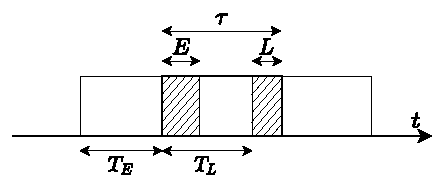
\includegraphics{Figures/Ch5_PacketsRandomChannel.pdf}
    \else
        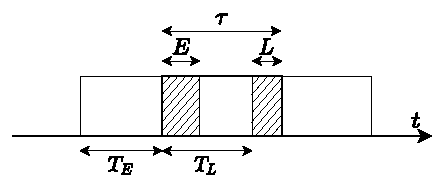
\includegraphics[draft]{Figures/Ch5_PacketsRandomChannel.pdf}
    \fi
    \caption{An early and late interfering packets with respect to the typical packet. The hachured regions correspond to packet overlapping. If $E+L>\beta\tau$, then the packet transmission fails.}
    \label{fig:P2_diagram_ECC}
\end{figure}%

~\\

\begin{theorem} \label{th:F_S0}
    The cumulative distribution function of $\overline{S_0}$ is
    \begin{align*}
        F_{\overline{S_0}}(x) = 
        \begin{cases}
            0, & \text{if } x < 0, \\
            (1 + \upsilon\,x)\,\euler^{-\upsilon\,(2-x)}, & \text{if } 0 \le x < 1,\\
            1, & \text{if } x \ge 1,
        \end{cases}
    \end{align*}
    where $\upsilon = \lambda\tau$.
\end{theorem}
%
\begin{proof}
    Since $\Pi$ is a Poisson point process on $\R$, the inter-arrival times follow iid exponential distributions of parameter $\lambda$. This can be shown through the void probabilities of the PPP, i.e., $\P(\Pi((0,t))=0) = \euler^{-\lambda t}$.
    
    Let the inter-arrival time of the early interferer and the late interferer be represented by the random variables $T_E\sim\mathscr{E}(\lambda)$ and $T_L\sim\mathscr{E}(\lambda)$, respectively.
    %
    Then, the superposition of the late interfering packet with the typical packet is given by $L = (\tau - T_L)_+$, where $(\cdot)_+ = \max\{\cdot,0\}$ as illustrated in Fig.~\ref{fig:P2_diagram_ECC}. Analogously for the early interferer $E = (\tau - T_E)_+$.
    %
    Thus, the cdf of $E$ and $L$ is
    \[
        F_E(t) = F_L(t) = % \ind\{t > \tau\} + \ind\{0\le t \le \tau\} \euler^{-\lambda(\tau-t)} =
        \begin{cases}
            0, &\text{if } t < 0 \\
            \euler^{-\lambda(\tau-t)}, &\text{if } 0 \le t < \tau,\\
            1, &\text{if } t \ge \tau.
        \end{cases}
    \]
    Note there is a discontinuity at $t=0$, thus the density does not exist with respect to the Lebesgue measure. Then, it is convenient to use the Lebesgue–-Stieltjes notation (Definition~\ref{def:lebesgue-stieltjes}).
    
    From \eqref{eq:ECC_I} we can see that $\overline{S_0}\,\tau = \max\{E+L,\tau\}$. Thus, for $x\in[0,1)$, we have that
    \begin{align*}
        \qquad 
        \P(\overline{S_0} \le x)
            &= \P(\max\{E+L,\tau\} \le x\,\tau) \\
            &= \P(E+L \le x\,\tau) &&\hspace{-10mm}\text{as }\tau > x\,\tau\\
            &= \int F_E(x\,\tau - t)\,\d F_L(t) &&\hspace{-10mm}\text{as $E$ and $L$ are independent}\\
            &= \euler^{-\lambda(\tau-x\,\tau)} \euler^{-\lambda\tau} + \int_0^{x\,\tau} \euler^{-\lambda(\tau-x\,\tau+t)} \lambda\euler^{-\lambda(\tau-t)}\d t \\
            &= (1+\lambda\tau\,x)\,\euler^{-\lambda\tau(2-x)}.
    \end{align*}
    The cases for which $x\notin[0,1)$ are trivial.
\end{proof}

% Note that the random variable $\overline{S_0}$ does not admit a density with respect to the Lebesgue measure, because of the discontinuities of the cdf at $0$ and $1$, that is why we used the Lebesgue--Stieltjes notation.

\begin{proposition}
	In the ECC model, where $\beta\in[0,1)$, the transmission success probability and throughput is given, respectively, by
    \begin{align*} \label{AlohaECC_thr}
        p_s     &= (1 + \beta\,\upsilon)\,\euler^{-(2-\beta)\,\upsilon},\\
    	\mathscr{T} &= \upsilon\,(1 + \beta\,\upsilon)\,\euler^{-(2-\beta)\,\upsilon},
    \end{align*}
    where $\upsilon = \lambda\tau$ is the occupation rate of the channel.
    
    Further, the unique and global maximum throughput is achieved when $\upsilon = \upsilon^*$, where
    \begin{equation*} \label{AlohaECC_max}
	    \upsilon^* = \frac{\sqrt{(2-\beta)^2+4\beta^2}-(2-3\beta)}{2\beta\,(2-\beta)}.
    \end{equation*}
\end{proposition}
\begin{proof}
    The transmission success probability and throughput follow directly from Theorem~\ref{th:F_S0} along with $p_s = \P(\overline{S_0}\le\beta) = F_{\overline{S_0}}(\beta)$ and $\mathscr{T} = \lambda\tau\,p_s$.
    
    Then, we use Theorem~\ref{th:unique_opt} to verify that the throughput has a unique local maximum which is a global maximum.
\end{proof}

If we let $\beta = 0$ in the ECC model we recover the unslotted ALOHA model \cite{abramson1970aloha}.
%
On the other hand, to achieve the maximum throughput of the slotted ALOHA, which is $1/\euler$, we must have $\beta \approx 0.56$.

Figures \ref{fig:P2_ECC} and \ref{fig:P2_ECC_ps} show the throughput $\mathscr{T}$ as a function of the traffic $\upsilon$ and as a function of the transmission success probability $p_s$, respectively.
%
As expected, the throughput grows when the system is more robust (when $\beta$ increases), even if we consider a fixed transmission success probability.

\begin{figure}[htb]
    \centering
    \if\printfig1
        % 
\begin{tikzpicture}[scale=1.0]

\begin{axis}
[
  title={},
  width  = 0.8*\columnwidth, 
  height = 0.4*\columnwidth,
  legend style={at={(0.975,0.95)}, anchor=north east},
%   xmode=log,
  xlabel={$\upsilon = \lambda\tau$},
  ylabel={$\mathscr{T}$}, ylabel style={rotate=-90},
%  yticklabel=\pgfmathprintnumber{\tick}\\ \%,
  xmin = 0,
  xmax = 5,
  ymin = 0,
%   ymax = 3,
  x tick label style={
        /pgf/number format/.cd,
        fixed,
        fixed zerofill,
        precision=1,
        /tikz/.cd
  },
  grid = both,
  scale only axis,
]
	\legend{slotted ALOHA, unslotted ALOHA, ECC model}
    
    \addplot[thick, blue, domain = 0:5, samples=100] {x*exp(-x)};
    \addplot[thick, red, domain = 0:5, samples=100] {x*exp(-2*x)};
    
    \foreach \a in {0.1,0.2,0.3,0.4,0.5,0.6}
        \addplot[domain = 0:5, samples=100] {x*(1+\a*x)*exp(-(2-\a)*x)};
    
    % \addplot[domain = 0.5:1.04, dashed, samples=100] {x*(1+((-3 + 2*x + sqrt(5 + 4*(-1 + x)*x))/(2*x))*x)*exp(-(2-((-3 + 2*x + sqrt(5 + 4*(-1 + x)*x))/(2*x)))*x)};
    
%     \addplot[thick] table
%     [
% 		x expr = \thisrow{lam},
%     	y expr = \thisrow{25dB}
%     ] {./Data/envelopes.dat};

    \draw[-\arrowhead] (axis cs: 0.8,0.08) -- (axis cs: 2.5,0.27) node[anchor= west] 
        {$\beta = 0.1,0.2,0.3,0.4,0.5,0.6$};
\end{axis}

\end{tikzpicture}

        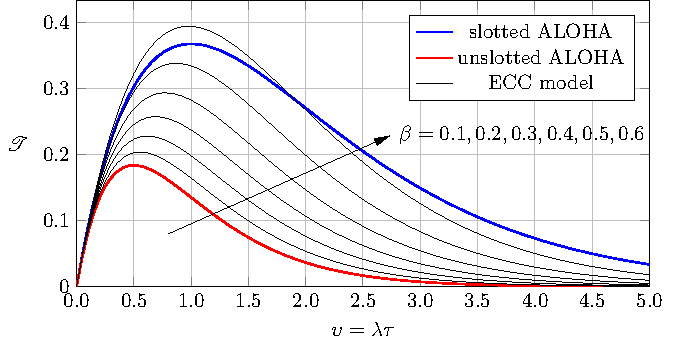
\includegraphics[]{Figures/Ch5_ECC.pdf}
    \else
        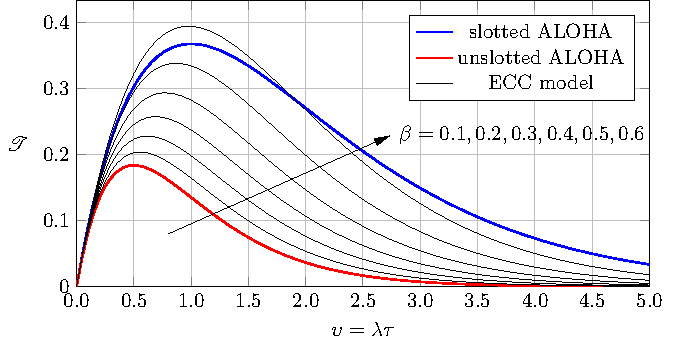
\includegraphics[draft, width=\textwidth]{Figures/Ch5_ECC.pdf}
    \fi
    \caption{Throughput $\mathscr{T}$ of the ECC model as a function of occupation rate of the channel $\upsilon$ for different values of $\beta$.}
    \label{fig:P2_ECC}
\end{figure}%
%
\begin{figure}[htb]
    \centering
    \if\printfig1
        % 
\begin{tikzpicture}[scale=1.0]

\begin{axis}
[
  title={},
  width  = 0.8*\columnwidth, 
  height = 0.4*\columnwidth,
  legend style={at={(0.975,0.95)}, anchor=north east},
%   xmode=log,
  xlabel={$p_s$},
  ylabel={$\mathscr{T}$}, ylabel style={rotate=-90},
%  yticklabel=\pgfmathprintnumber{\tick}\\ \%,
  xmin = 0,
  xmax = 1,
  ymin = 0,
%   ymax = 3,
  x tick label style={
        /pgf/number format/.cd,
        fixed,
        fixed zerofill,
        precision=1,
        /tikz/.cd
  },
  grid = both,
  scale only axis,
]
	\legend{slotted ALOHA, unslotted ALOHA, ECC model}
    
    \addplot[thick, blue, domain = 0:5, samples=100] ({exp(-x)},{x*exp(-x)});
    \addplot[thick, red, domain = 0:5, samples=100] ({exp(-2*x)},{x*exp(-2*x)});
    
    \foreach \a in {0.1,0.2,0.3,0.4,0.5,0.6}
        % \addplot[domain = 0:5, samples=100] {x*(1+\a*x)*exp(-(2-\a)*x)};
        \addplot [domain=0:5, samples=100, black] ({(1+\a*x)*exp(-(2-\a)*x)}, {x*(1+\a*x)*exp(-(2-\a)*x)});
    
    % \addplot[domain = 0.5:1.04, dashed, samples=100] {x*(1+((-3 + 2*x + sqrt(5 + 4*(-1 + x)*x))/(2*x))*x)*exp(-(2-((-3 + 2*x + sqrt(5 + 4*(-1 + x)*x))/(2*x)))*x)};
    
%     \addplot[thick] table
%     [
% 		x expr = \thisrow{lam},
%     	y expr = \thisrow{25dB}
%     ] {./Data/envelopes.dat};

    \draw[\arrowhead-] (axis cs: 0.9,0.2) -- (axis cs: 0.7,0.08) node[anchor= east] 
        {$\beta = 0.1,0.2,0.3,0.4,0.5,0.6$};
\end{axis}

\end{tikzpicture}

        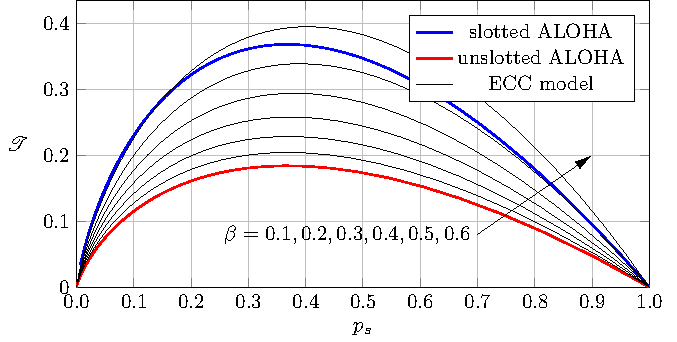
\includegraphics[]{Figures/Ch5_ECC_ps.pdf}
    \else
        
\includegraphics[draft, width=\textwidth]{Figures/placeholder.png}
    \fi
    \caption{Parametric curve of the throughput $\mathscr{T}$ and the transmission success probability $p_s$ as we vary $\upsilon$ in the ECC model for different values of $\beta$.}
    \label{fig:P2_ECC_ps}
\end{figure}

% % % % % % % % % % % % % % % % % % % % % 
\section{Average Interference model}
\label{sec:AI_model}

In the Average Interference model (AI model) we assume that a packet is successfully transmitted if the average of the received interference does not exceed the threshold $\beta \ge 0$.
%
Thus, the transmission success probability is given by $p_s = \P(\overline{I_0}\le\beta)$, where the random variable $\overline{I_0}$ is the mean interference on the typical packet and is defined as
\begin{align}\label{eq:AI_I}
    \overline{I_0} \triangleq \frac{1}{\tau}\int_0^\tau I_0(t)\,\d t.
\end{align}

\begin{theorem} \label{th:F_I0}
    The cumulative distribution function of $\overline{I_0}$ is given by the finite sum
    \begin{equation*}
    	F_{\overline{I_0}}(x) = \euler^{-2\upsilon} \sum_{k=0}^{\lfloor x \rfloor} \dfrac{(-1)^k}{k!} \left(\sqrt{2\,\upsilon\,(x-k)}\right)^k \cal{I}_k\!\left(\sqrt{8\,\upsilon\,(x-k)}\right),\quad x \geq 0,
    \end{equation*}
    where $\cal{I}_k$ is the $k$th order modified Bessel function of the first kind\footnote{Let $k\in\N$. The $k$th order modified Bessel function of the first kind is defined as \vspace{-2mm}\[\cal{I}_k(x) \triangleq \frac{1}{\pi}\int_0^\pi \euler^{x\cos\theta}\cos(k\theta)\,\d\theta,\quad x\in\R.\vspace{-3mm}\]}, $\lfloor \cdot \rfloor$ is the floor function\footnote{The floor function returns the biggest integer less than or equal to the argument.}, and $\upsilon = \lambda\tau$.
\end{theorem}
\begin{proof}
    From \eqref{eq:interf_I0} and \eqref{eq:AI_I}, we have that
    \begin{align*}\label{eq:AI_I}
        \overline{I_0} 
            &= \frac{1}{\tau}\int_0^\tau \sum_{x\in\Pi} \ind_{[0,\tau]}(t-x)\,\d t \\
            &= \frac{1}{\tau}\sum_{x\in\Pi} \int_0^\tau  \ind_{[0,\tau]}(t-x)\,\d t \\
            &= \frac{1}{\tau}\sum_{x\in\Pi\cap[-\tau,\tau]} (\tau - |x|),
    \end{align*}
    where we used the Fubini--Tonelli theorem (Theorem~\ref{th:fubini-tonelli}) to interchange the sum with the integral, because we have positive terms.
    %
    Note that the term $(\tau - |x|)$ gives the superposition time between an interfering packet and the typical packet.
    
    Now, using the Campbell theorem (Theorem~\ref{th:campbell}) we have that the Laplace--Stieltjes transform of the distribution of $\overline{I_0}$ is
    \begin{align*}
    	\E\!\left[\euler^{-s \overline{I_0}}\right]	&= \exp\!\left[ -\int_{-\tau}^\tau(1-\euler^{-s(1-|x|/\tau)}) \,\lambda\,dx \right] \\
        				&= \exp\!\left[ -2\upsilon\left( 1 - \frac{1-\euler^{-s}}{s} \right) \right],\quad s\in\C \backslash \{0\},
    \end{align*}
    where we used that the traffic $\upsilon = \lambda\tau$.
    
    Using the power series expansion of the exponential function on $\exp(-2\upsilon\,\euler^{-s}/s)$ and dividing by $s$ both sides of the equation, we can rewrite it as
    \begin{equation*}
    	\frac{1}{s}\E\!\left[\euler^{-s \overline{I_0}}\right] = \euler^{-2\upsilon} \sum_{k\geq0} \frac{(-2\upsilon)^k}{k!} \frac{\euler^{2\upsilon/s}}{s^{k+1}}\,\euler^{-k s},\quad s\in\C \backslash \{0\}.
    \end{equation*}
    
    % Para $k$ suficientemente grande, os valores absolutos dos termos dessa série podem ser limitados por cima pela função $e^-s$. Logo, podemos aplicar o teorema da convergência dominada para calcular a transformada de Laplace–Stieltjes inversa termo a termo.
    %Aplicando a transformada inversa de Laplace–Stieltjes nos dois lados da equação e usando o Teorema da convergência dominada de Lebesgue \cite[Teorema~1.34]{rudin1987real} para trocar o limite da soma com a transformada inversa, obtemos a c.d.f. de $\overline{I_0}$,
    Then, we apply the inverse Laplace–-Stieltjes transform on both sides of the equation to obtain the cdf of $\overline{I_0}$, which concludes the proof.
\end{proof}

\begin{proposition}
In the AI model with $\beta\in[0,1]$, the transmission success probability and throughput is given, respectively, by
\begin{align*}
    p_s &= \cal{I}_0\!\left( \sqrt{8\,\beta\,\upsilon} \right) \euler^{-2\,\upsilon},\\
	\mathscr{T} &= \upsilon\,\cal{I}_0\!\left( \sqrt{8\,\beta\,\upsilon} \right) \euler^{-2\,\upsilon},
\end{align*}
where $\cal{I}_0$ is the zeroth order modified Bessel function of the first kind.

For $\beta \ge 0$, then $p_s = F_{\overline{I_0}}(\beta)$ and $\mathscr{T} = \upsilon\,p_s$, where $F_{\overline{I_0}}$ is given by Theorem~\ref{th:F_I0}.
\end{proposition}

\begin{proof}
We know that the packet success probability $p_s = \P(\overline{I_0}\leq \beta) = F_{\overline{I_0}}(\beta)$ and throughput $\mathscr{T} = \upsilon\,p_s$.
%
Now, note that if $\beta\in[0,1]$, then the sum in Theorem~\ref{th:F_I0} consists of a single term.
\end{proof}

Since $\cal{I}_0(0) = 1$, we recover the classical result of the unslotted ALOHA for $\beta = 0$ as expected.
%
On the other hand, to achieve the maximum throughput of the slotted ALOHA, we need to have $\beta\approx0.621$.

Analogously to the ECC model, Figures \ref{fig:P2_AI} and \ref{fig:P2_AI_ps} show the throughput $\mathscr{T}$ as a function of the traffic $\upsilon$ and as a function of the transmission success probability $p_s$, respectively.
%
Again, we observe the same behavior that the throughput grows when the system is more robust ($\beta$ increases).

Furthermore, for the same $\beta$ and $\upsilon$, we have that the transmission success probability of the ECC model is bigger than the one of the AI model. This happens because $\overline{S_0} \le \overline{I_0}$.

\begin{figure}[htb]
    \centering
    \if\printfig1
        % 
\begin{tikzpicture}[scale=1.0]

\begin{axis}
[
  title={},
  width  = 0.8*\columnwidth, 
  height = 0.4*\columnwidth,
  legend style={at={(0.975,0.95)}, anchor=north east},
%   xmode=log,
  xlabel={$\upsilon=\lambda\tau$},
  ylabel={$\mathscr{T}$}, ylabel style={rotate=-90},
%  yticklabel=\pgfmathprintnumber{\tick}\\ \%,
  xmin = 0, 	
  xmax = 5,
  ymin = 0, 	
%   ymax = 3,
  x tick label style={
        /pgf/number format/.cd,
        fixed,
        fixed zerofill,
        precision=1,
        /tikz/.cd
  },
  grid = both,
  scale only axis,
]
	\legend{slotted ALOHA, unslotted ALOHA, AI model}
    
    \addplot[thick, blue, domain = 0:5, samples=100] {x*exp(-x)};
    \addplot[thick, red, domain = 0:5, samples=100] {x*exp(-2*x)};
    
    \foreach \e in {0.1,0.2,0.3,0.4,0.5,0.6,0.7}
        \addplot[domain = 0:5, samples=100] {x*exp(-2*x)*cosh(sqrt(8*\e*x))/(1+8*\e*x/4)^(1/4)*(1+0.24273*8*\e*x)/(1+0.43023*8*\e*x)};
    
    % \addplot[domain = 0.5:1.04, dashed, samples=100] {x*(1+((-3 + 2*x + sqrt(5 + 4*(-1 + x)*x))/(2*x))*x)*exp(-(2-((-3 + 2*x + sqrt(5 + 4*(-1 + x)*x))/(2*x)))*x)};
    
%     \addplot[thick] table
%     [
% 		x expr = \thisrow{lam},
%     	y expr = \thisrow{25dB}
%     ] {./Data/envelopes.dat};

    \draw[-\arrowhead] (axis cs: 0.8,0.08) -- (axis cs: 2.7,0.25) node[anchor= west] 
        {$\beta = 0.1,0.2,0.3,0.4,0.5,0.6,0.7$};
\end{axis}

\end{tikzpicture}

        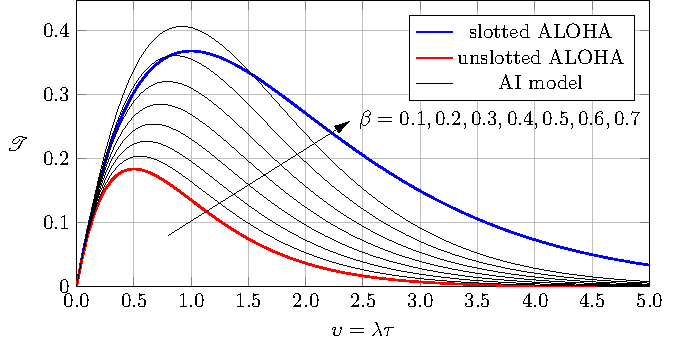
\includegraphics[]{Figures/Ch5_AI.pdf}
    \else
        
\includegraphics[draft, width=\textwidth]{Figures/placeholder.png}
    \fi
    \caption{Throughput $\mathscr{T}$ of the AI model as a function of occupation rate of the channel $\upsilon$ for different values of $\beta$.}
    \label{fig:P2_AI}
\end{figure}%
%
\begin{figure}[htb]
    \centering
    \if\printfig1
        % 
\begin{tikzpicture}[scale=1.0]

\begin{axis}
[
  title={},
  width  = 0.8*\columnwidth, 
  height = 0.4*\columnwidth,
  legend style={at={(0.975,0.95)}, anchor=north east},
%   xmode=log,
  xlabel={$p_s$},
  ylabel={$\mathscr{T}$}, ylabel style={rotate=-90},
%  yticklabel=\pgfmathprintnumber{\tick}\\ \%,
  xmin = 0, 	
  xmax = 1,
  ymin = 0, 	
%   ymax = 3,
  x tick label style={
        /pgf/number format/.cd,
        fixed,
        fixed zerofill,
        precision=1,
        /tikz/.cd
  },
  grid = both,
  scale only axis,
]
	\legend{slotted ALOHA, unslotted ALOHA, AI model}
    
    \addplot[thick, blue, domain = 0:5, samples=100] ({exp(-x)},{x*exp(-x)});
    \addplot[thick, red, domain = 0:5, samples=100] ({exp(-2*x)},{x*exp(-2*x)});
    
    \foreach \e in {0.1,0.2,0.3,0.4,0.5,0.6,0.7}
        \addplot[domain = 0:5, samples=100]
        ({exp(-2*x)*cosh(sqrt(8*\e*x))/(1+8*\e*x/4)^(1/4)*(1+0.24273*8*\e*x)/(1+0.43023*8*\e*x)},
        {x*exp(-2*x)*cosh(sqrt(8*\e*x))/(1+8*\e*x/4)^(1/4)*(1+0.24273*8*\e*x)/(1+0.43023*8*\e*x)});
    
    % \addplot[domain = 0.5:1.04, dashed, samples=100] {x*(1+((-3 + 2*x + sqrt(5 + 4*(-1 + x)*x))/(2*x))*x)*exp(-(2-((-3 + 2*x + sqrt(5 + 4*(-1 + x)*x))/(2*x)))*x)};
    
%     \addplot[thick] table
%     [
% 		x expr = \thisrow{lam},
%     	y expr = \thisrow{25dB}
%     ] {./Data/envelopes.dat};

    \draw[\arrowhead-] (axis cs: 0.9,0.2) -- (axis cs: 0.7,0.08) node[anchor= east] 
        {$\beta = 0.1,0.2,0.3,0.4,0.5,0.6,0.7$};
\end{axis}

\end{tikzpicture}

        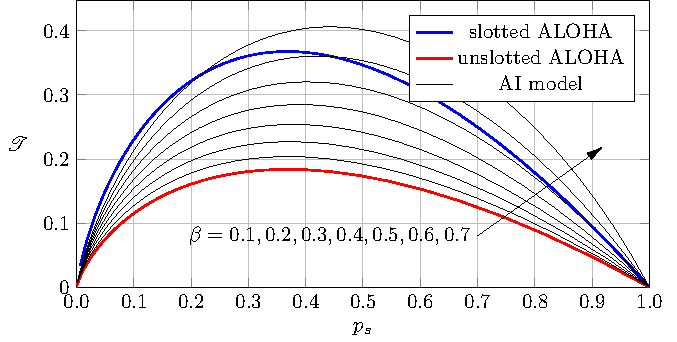
\includegraphics[]{Figures/Ch5_AI_ps.pdf}
    \else
        
\includegraphics[draft, width=\textwidth]{Figures/placeholder.png}
    \fi
    \caption{Parametric curve of the throughput $\mathscr{T}$ and the transmission success probability $p_s$ as we vary $\upsilon$ in the AI model for different values of $\beta$.}
    \label{fig:P2_AI_ps}
\end{figure}

% % % % % % % % % % % % % % % % % % % % % 
\section{High Interference model}
\label{sec:HI_model}

In the High Interference model (HI model) we assume that a packet is successfully transmitted if the proportion of the packet that was affected by \textit{high interference} is smaller than or equal to $\beta\in[0,1]$. We define the period of \textit{high interference} as the times for which the number of interfering packets is greater than a threshold $h\in\N$.

Thus, the transmission success probability is given by $p_s = \P\!\left(\overline{S_h} \le \beta\right)$, where $\overline{S_h}$ is the proportion of time the typical packet was affected by \textit{high interference} and is defined as
\begin{align}\label{eq:Sh_def}
    \overline{S_h} \triangleq \frac{1}{\tau}\int_0^\tau \ind\{I_0(t) > h\}\,\d t.
\end{align}

Considering every $h\in\N$, the distribution of the random variable $\overline{S_h}$ would provide a thorough characterization of the stochastic process $\{I(t)\}_t$,
%
because it would capture every interference level and the distribution of its duration in the typical packet.
%
However, as we shall see, the distribution of $\overline{S_h}$ is quite intricate.

\begin{remark} \label{remark:Ch5_ineq}
    The HI model is a generalization of the ECC model because we recover the latter by making $h=0$ in the former.
    %
    Also, one can show that the HI model is related to the AI model through the following identity
    \begin{align*}
        \sum_{h\ge 0} \overline{S_h} = \overline{I_0}.
    \end{align*}
    Furthermore, $\overline{S_0} \ge \overline{S_1} \ge \cdots$.
\end{remark}

Let the number of interferers that start transmitting during the transmission of the typical packet be represented by the random variable $LI$ (late interferers) and the number of interferers that stop transmitting during the transmission of the typical packet be represented by the random variable $EI$ (early interferers), i.e.,
\begin{align*}
    EI \triangleq I_0(0) \sim \mathscr{P}(\lambda\tau), \qquad LI \triangleq I_0(\tau) \sim \mathscr{P}(\lambda\tau).
\end{align*}
Then, since $\Pi$ is a Poisson point process, it is easy to see that $EI$ and $LI$ are independent and follow a Poisson distribution of parameter $\upsilon = \lambda\tau$.

Let $(t_k)_{k=1}^{EI+LI}$ be the sequence of times for which an interferer stops or starts a transmission.
%
Then, it is possible to uniquely determine $\{I(t)\}_t$ from the sequences $(t_1,\dots,t_{EI+LI})$ and $(I(0),I(t_1),\dots,I(t_{EI+LI}))$.
%
Furthermore, the proportion of time the typical packet was affected by \textit{high interference} can be written as
\begin{align} \label{eq:ch5_Sh}
    \overline{S_h}
        &= \sum_{k=0}^{EI+LI} \dfrac{\Delta t_k}{\tau}\,\ind{\{I(t_k) > h\}},
\end{align}
where $\Delta t_k \triangleq t_{k+1} - t_{k}$ and we use $t_0 = 0$, $t_{EI+LI+1} = \tau$.

Given $EI = k$ and $LI = l$, the distribution of the $k+l$ times of starting or stopping a transmission are independent and uniformly distributed on $[0,\tau)$. 
\begin{note}
    We can check the above-mentioned property by showing the random variable that represents the number of points of the PPP that are in a subset $T$ of $[0,\tau)$ follow a binomial distribution of parameters $(k+l,\mu(T))$, where $\mu(T)$ is the length of the subset.
    
    To prove this property in a more general form, it is enough to show that for every $A,B\in\cal{B}(\R)$ such that $A\subset B$ the random variable $\Pi(A)|\Pi(B)$ follows a binomial distribution of parameters $(\Pi(B), \mu(A)/\mu(B))$ , where $\mu$ is the Lebesgue measure.
\end{note}

Further, the random vector $(I(t_i))_{i=0}^{k+l}$ is a symmetric Bernoulli random walk\footnote{A symmetric Bernoulli random walk is a random walk on $\Z$ that performs unitary steps and each step has equal probability of being $+1$ or $-1$.} subject to begin at $k$ and end at $l$ with $k+l$ steps.
%
% In this random walk, every path is equiprobable.
The total number of different paths is given by the binomial coefficient $\binom{k+l}{k}$.
%
We are interested to know how many of these paths stay a total number of $m\in\N$ steps above the threshold $h$. Let us denote the number of paths that satisfy this as $C_{k,l}^{h,m}\in\N$.
%
Formally, we can write that
\begin{align} \label{eq:Ch5_Cklhm}
    C_{k,l}^{h,m} \triangleq \sum_{\bm{x}\in\mathscr{X}_{k,l}}\ind
        \!\left\{ \sum_{i=0}^{k+l} \ind\{x_i > h\} = m\right\},
\end{align}
where $\mathscr{X}_{k,l} \subset \N^{k+l+1}$ is the set that contains all paths from $k$ to $l$ with $k+l$ unit steps.

Now we can express the probability of having exactly $m$ times of the random vector $(t_i)_{i=0}^{k+l}$ for which the typical packet is affected by an interference greater than $h$ as $C_{k,l}^{h,m}/\binom{k+l}{k}$.

Fig.~\ref{fig:random_walk} illustrate some random walks that starts at $k=5$ and end at $l=3$ in $k+l=8$ steps. We show $3$ of the $\binom{8}{3} = 56$ possible paths.
%
Note that for this case, the only path that surpass $h=7$ (\textit{high interference}) is the red path and it stays above $h$ for only $m=1$ step.
%
Indeed, $C_{5,3}^{7,m} = \ind\{m=1\}$, thus there is only one path that does that.
\begin{figure}[htb]
\centering
    \if\printfig1
        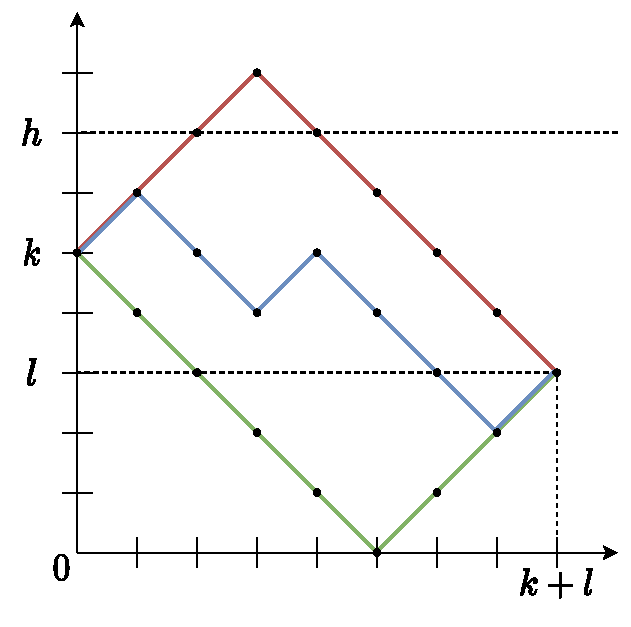
\includegraphics[width=0.45\textwidth]{Figures/Ch5_RandomWalk.pdf}
    \else
        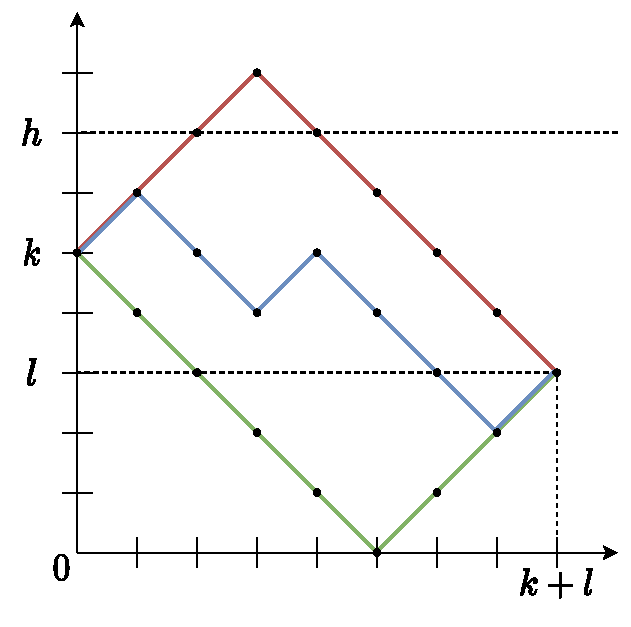
\includegraphics[draft, width=0.5\textwidth]{Figures/Ch5_RandomWalk.pdf}
    \fi
	\caption{Examples of random walks starting at $k=5$ and finishing at $l = 3$.}
	\label{fig:random_walk}
\end{figure}
%
It is worth remembering that in the original problem the $i$th step of the random walk stays in the corresponding state a time given by the random variable $\Delta t_i$.

Different from the other models, the HI model is much more complex, because the calculation of $C_{k,l}^{h,m}$ is done case by case despite having a (strictly speaking) \textit{closed form} expression.
%
As we shall see, we need $C_{k,l}^{r,m}$ for an infinite number of argument combinations and, then, we stumble upon a difficult problem.

\begin{remark} \label{rem:Ch5_Crmkl}
    On the other hand, we can find simple formulas for some special argument values of $C_{k,l}^{r,m}$ as follows.
    \begin{itemize}
        \item $C_{k,l}^{r,m} = C_{l,k}^{r,m}$ by symmetry;
        
        \item If $k\leq r$ and $l\leq r$, then $C_{k,l}^{r,0} = \binom{k+l}{k} - \binom{k+l}{r+1}$ by the reflection method \cite{feller1968introduction};
        
        \item If $k>r$ and $l>r$, then $C_{k,l}^{r,k+l+1} = \binom{k+l}{k} - \binom{k+l}{r}$ by the reflection method again;
        
        \item If $k\leq r$ and $k+l-(r-k) \leq m \leq k+l$, then $C_{k,l}^{r,m}=0$,
    \end{itemize}
    where we consider the binomial coefficient $\binom{n}{k} = 0$ when $k \notin \{0,1,\dots,n\}$.
\end{remark}

Assuming that we have $m$ intervals of time with \textit{high interference}, then we need to find the probability that the sum of $m$ intervals of \textit{high interference} is smaller or equal than $\beta\tau$, which is the condition for successful transmission.
%
Indeed, we have that
\[
    \P(\Delta t_0 + \Delta t_1 + \cdots + \Delta t_{m-1} \leq \beta\tau) = \cal{P}_{k+l,m}(\beta),
\]
where
\begin{align} \label{eq:Ch5_Pdef}
    \cal{P}_{n,m}(x) \triangleq
    \begin{cases}
        \ind\{m = 0\}, &\text{if } x = 0,\\
        \displaystyle\sum_{i=m}^{n} \binom{n}{i}x^i(1-x)^{n-i}, &\text{if } x\in(0,1),\\
        1, &\text{if } x = 1,
    \end{cases}
\end{align}
because we have $k+l$ independent random variables uniformly distributed on $[0,\tau)$ and we want that at least $m$ of them are in the interval $[0,\beta\tau]$.
%
From order statistics theory we can generalize this result to
\begin{align} \label{eq:ch5_Pdeltat}
	\P(\Delta t_{\nu(0)} + \Delta t_{\nu(1)} + \cdots + \Delta t_{\nu(m-1)} \leq \beta\tau) = \cal{P}_{k+l,m}(\beta),
\end{align}
where $\nu:\{0,1,\cdots,m-1\} \longrightarrow \{0,1,\cdots,k+l\}$ is an arbitrary injective function.
%
This takes into account the cases where the intervals of \textit{high interference} are not contiguous.

Finally, we can conclude from \eqref{eq:ch5_Sh} and \eqref{eq:ch5_Pdeltat} that
\begin{align} \label{eq:Ch5_Sh_EIEL}
    \P(\overline{S_h} \leq x~|~EI=k,LI=l) 
	    &= \sum_{m=0}^{k+l+1} \dfrac{C_{k,l}^{r,m}}{\binom{k+l}{k}} \cal{P}_{k+l,m}(x), \quad x\in[0,1].
\end{align}

Now, we are prepared to prove the following theorem.
\begin{theorem} \label{th:F_Sh}
    The cumulative distribution function of $\overline{S_h}$, $h\in\N$, is
    \begin{align*}
        F_{\overline{S_h}}(x)
            &= \euler^{-2\upsilon} \sum_{n \geq 0} \frac{\upsilon^n}{n!} \sum_{m=0}^{n+1}  \cal{P}_{n,m}(x) \sum_{k=0}^n C^{h,m}_{k,n-k}, \quad x\in[0,1],
    \end{align*}
    where $\upsilon = \lambda\tau$, $C$ is defined in \eqref{eq:Ch5_Cklhm} and $\cal{P}$ is defined in \eqref{eq:Ch5_Pdef}.
    
    Further, we can express the probabilities at the discontinuities of $F_{\overline{S_h}}$ in \textit{closed form}:
    \begin{align*}
        \P(\overline{S_h}=0) 
            &= \left( f_{h}(\upsilon) \right)^2 + (\upsilon-h) \frac{\upsilon^{h+1}\euler^{-\upsilon}}{(h+1)!} f_{h}(\upsilon)  - \dfrac{\upsilon^{2(h+1)}\euler^{-2 \upsilon}}{h!(h+1)!},\\
        \P(\overline{S_h}=1) 
            &= \left( 1 - f_{h}(\upsilon) \right)^2 + (h+1-\upsilon) \left( 1 - f_{h-1}(\upsilon) \right) \frac{\upsilon^h \euler^{-\upsilon}}{h!} -(h+1)\frac{\upsilon^{2h}\euler^{-2\upsilon}}{(h!)^2},
    \end{align*}
    where $f_h(\upsilon)\triangleq \euler^{-\upsilon}\displaystyle\sum_{k=0}^{h}\frac{\upsilon^h}{h!}$.
\end{theorem}
\begin{proof}
    We know that the random variables $EI$ and $LI$ follow a Poisson distribution of parameter $\upsilon=\lambda\tau$. Thus, we can decondition \eqref{eq:Ch5_Sh_EIEL} on $EI$ and $LI$ to obtain, for $x\in[0,1]$,
    \begin{align}
    	\P(\overline{S_h} \leq x)
    	    &= \euler^{-2\upsilon}\sum_{k \geq 0}\sum_{l \geq 0} \frac{\upsilon^{k+l}}{k!l!}\sum_{m=0}^{k+l+1} \dfrac{C_{k,l}^{r,m}}{\binom{k+l}{k}} \cal{P}_{k+l,m}(x) \label{eq:Ch5_F_Sh_aux1}\\
    		&= \euler^{-2\upsilon}\sum_{k \geq 0}\sum_{l \geq 0} \frac{\upsilon^{k+l}}{(k+l)!}\sum_{m=0}^{k+l+1} C_{k,l}^{r,m} \cal{P}_{k+l,m}(x) \label{eq:Ch5_F_Sh_aux2}\\
        	&= \euler^{-2\upsilon}\sum_{n \geq 0} \sum_{m=0}^{n+1}  \sum_{k=0}^n C^{r,m}_{k,n-k} \cal{P}_{n,m}(x)  \frac{\upsilon^n}{n!},
    \end{align}
    where we performed the variable change $l=n-k$ and we can interchange the sums because all terms are positive (Fubini–-Tonelli theorem, Theorem~\ref{th:fubini-tonelli}).
    %
    This proves the first result because $F_{\overline{S_h}}(x) = \P(\overline{S_h} \le x).$
    
    Now, using \eqref{eq:Ch5_F_Sh_aux2} and Remark~\ref{rem:Ch5_Crmkl} we have that
    \begin{align*}
    \P(\overline{S_h} = 0)
    	 &= \euler^{-2\upsilon}\sum_{k \geq 0}\sum_{l \geq 0} \frac{\upsilon^{k+l}}{(k+l)!}\sum_{m=0}^{k+l} C_{k,l}^{h,m} \cal{P}_{k+l,m}(0)\\
         &= \euler^{-2\upsilon}\sum_{k \geq 0}\sum_{l \geq 0} \frac{\upsilon^{k+l}}{(k+l)!} C_{k,l}^{h,0}\\
         &= \euler^{-2\upsilon}\sum_{k \geq 0}\sum_{l \geq 0} \frac{\upsilon^{k+l}}{(k+l)!} \left( \binom{k+l}{k} - \binom{k+l}{h+1} \ind_{\{k+l > h\}} \right)\ind_{\{k \leq h\}}\ind_{\{l \leq h\}}\\
         &= \euler^{-2\upsilon}\sum_{k = 0}^h \sum_{l = 0}^h \frac{\upsilon^{k+l}}{k!l!} \left( 1 - \frac{\binom{k+l}{h+1}}{\binom{k+l}{k}} \right).
    \end{align*}
    %
    Now, using $f_h$ and some tedious manipulations we find the \textit{closed form} of $\P(\overline{S_h} = 0)$.
    
    Using \eqref{eq:Ch5_F_Sh_aux1} and Remark~\ref{rem:Ch5_Crmkl} we have that
    \begin{align*}
	\P(\overline{S_h}=1)
	    &= F_{\overline{S_h}}(1) - \lim_{x\uparrow 1} F_{\overline{S_h}}(x)\\
    	&= \euler^{-2\upsilon}\sum_{k > 0}\sum_{l > 0} \frac{\upsilon^{k+l}}{k!l!} \dfrac{C_{k,l}^{h,k+l+1}}{\binom{k+l}{k}}\\
    	&= \euler^{-2\upsilon} \sum_{k > 0}\sum_{l > 0} \frac{\upsilon^{k+l}}{k!l!} \left( 1 - \frac{\binom{k+l}{h}}{\binom{k+l}{k}} \right)\ind_{\{k>h\}}\ind_{\{l>h\}}\\
    	&= \euler^{-2\upsilon} \sum_{k > h}\sum_{l > h} \frac{\upsilon^{k+l}}{k!l!} \left( 1 - \frac{\binom{k+l}{h}}{\binom{k+l}{k}} \right).
    \end{align*}
    %
    Again, using $f_h$ and some tedious manipulations we find the \textit{closed form} of $\P(\overline{S_h} = 1)$.
\end{proof}

Using Theorem~\ref{th:F_Sh} we can find simple expressions for the probability of not receiving \textit{high interference} at all during a typical packet transmission, i.e., $\P(\overline{S_h} = 0)$, for $h=0,1,2,\dots$.
%
\begin{align*}
    \P(\overline{S_0} = 0) &= \euler^{-2\,\upsilon},\\
    \P(\overline{S_1} = 0) &= \left( 1+2\upsilon+{\upsilon}^{2}/2 \right){\euler^{-2\,\upsilon}} ,\\
    \P(\overline{S_2} = 0) &= \left( 1+2\,\upsilon+2\,\upsilon^2+(2/3)\,\upsilon^3+(1/12)\,\upsilon^4 \right){{\euler}^{-2\,\upsilon}},\\
                &~\,\vdots\\
    \P(\overline{S_h} = 0) &= \frac{\upsilon^{2h}\euler^{-2\upsilon}}{h!(h+1)!} + \cal{O}(\upsilon^{2h-1}\euler^{-2\upsilon}), \quad \text{as } \upsilon\to\infty.
\end{align*}

The same can be done for the case of receiving \textit{high interference} during all transmission, i.e., $\P(\overline{S_h} = 1)$.
%
\begin{align*}
    \P(\overline{S_0} = 1) &= 1 - (1+\upsilon)\,\euler^{-\upsilon},\\
    \P(\overline{S_1} = 1) &= (1-\euler^{-\upsilon})^2 - \upsilon^2\,\euler^{-\upsilon},\\
    \P(\overline{S_2} = 1) &= (1-(1+\upsilon)\,\euler^{-\upsilon})^2 + (1-\upsilon-\euler^{-\upsilon})\,\frac{\upsilon^2}{2}\,\euler^{-\upsilon},\\
        &~\,\vdots\\
    \P(\overline{S_h} = 1) &= 1 - \frac{\upsilon^{h+1}}{h!}\,\euler^{-\upsilon} + \cal{O}\left(\upsilon^h\euler^{-\upsilon}\right), \quad \text{as } \upsilon\to\infty.
\end{align*}

\begin{figure}[htb]
    \centering
    \if\printfig1
        \begin{subfigure}{.45\textwidth}
          \centering
            % 
\begin{tikzpicture}[scale=0.8]

\begin{axis}
[
  title={$\beta = 0$},
%   width  = 0.8*\columnwidth, 
%   height = 0.4*\columnwidth,
  legend style={at={(0.95,0.95)}, anchor=north east},
%   xmode=log,
  xlabel={$\upsilon=\lambda\tau$},
  ylabel={$p_s$}, ylabel style={rotate=-90},
%  yticklabel=\pgfmathprintnumber{\tick}\\ \%,
  xmin = 0, 	
  xmax = 5,
  ymin = 0, 	
  ymax = 1,
  x tick label style={
        /pgf/number format/.cd,
        fixed,
        fixed zerofill,
        precision=1,
        /tikz/.cd
  },
  grid = both,
  scale only axis,
]
% 	\legend{slotted ALOHA, unslotted ALOHA}
    
    \addplot[thick, blue, domain = 0:5, samples=100] {exp(-x)};
    \addplot[thick, red, domain = 0:5, samples=100] {exp(-2*x)};
    
    \addplot[domain = 0:5, samples=100] {(1+2*x+x^2/2)*exp(-2*x)};
    \addplot[domain = 0:5, samples=100] {(1+2*x+2*x^2+(2/3)*x^3+x^4/12)*exp(-2*x)};
    \addplot[domain = 0:5, samples=100] {(1+2*x+2*x^2+(4/3)*x^3+(11/24)*x^4+x^5/12+x^6/144)*exp(-2*x)};
    \addplot[domain = 0:5, samples=100] {(1+2*x+2*x^2+(4/3)*x^3+(2/3)*x^4+(13/60)*x^5+(2/45)*x^6+x^7/180+x^8/2880)*exp(-2*x)};
    
%     \addplot[thick] table
%     [
% 		x expr = \thisrow{lam},
%     	y expr = \thisrow{25dB}
%     ] {./Data/envelopes.dat};

    \draw[-\arrowhead] (axis cs: 1.5,0.1) -- (axis cs: 3.50,0.75) node[anchor=south] 
        {$h = 1, 2, 3, 4$};
\end{axis}

\end{tikzpicture}

            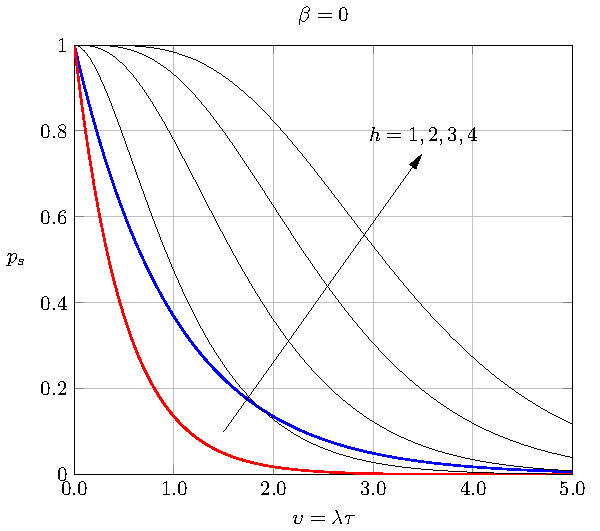
\includegraphics[width=\columnwidth]{Figures/Ch5_HI_0.pdf}
            % \caption{$\beta = 0$.}
        \label{fig:HI_0}
        \end{subfigure}%
        \begin{subfigure}{.05\textwidth}
        \hspace{.05\textwidth}
        \end{subfigure}%
        \begin{subfigure}{.45\textwidth}
          \centering
            % 
\begin{tikzpicture}[scale=0.8]

\begin{axis}
[
  title={$\beta\uparrow 1$},
%   width  = 0.8*\columnwidth, 
%   height = 0.4*\columnwidth,
  legend style={at={(0.95,0.95)}, anchor=north east},
%   xmode=log,
  xlabel={$\upsilon=\lambda\tau$},
  ylabel={$p_s$}, ylabel style={rotate=-90},
%  yticklabel=\pgfmathprintnumber{\tick}\\ \%,
  xmin = 0, 	
  xmax = 10,
  ymin = 0, 	
  ymax = 1,
  x tick label style={
        /pgf/number format/.cd,
        fixed,
        fixed zerofill,
        precision=1,
        /tikz/.cd
  },
  grid = both,
  scale only axis,
]
% 	\legend{slotted ALOHA, unslotted ALOHA}
    
    \addplot[thick, blue, domain = 0:10, samples=100] {exp(-x)};
    \addplot[thick, red, domain = 0:10, samples=100] {exp(-2*x)};
    
    \addplot[domain = 0:10, samples=100] {(1+x)*exp(-x)};
    \addplot[domain = 0:10, samples=100] {1-((1-exp(-x))^2-x^2*exp(-x))};
    \addplot[domain = 0:10, samples=100] {1-( (1-(1+x)*exp(-x))^2+(1-x-exp(-x))*x^2/2*exp(-x) )};
    \addplot[domain = 0:10, samples=100] {exp(-2*x)/12*(-12-24*x-24*x^2-8*x^3-x^4+2*exp(x)*(12+12*x+6*x^2-2*x^3+x^4))};
    \addplot[domain = 0:10, samples=100] {exp(-2*x)/144*(-144-288*x-288*x^2-192*x^3-66*x^4-12*x^5-x^6+6*exp(x)*( 48+48*x+24*x^2+8*x^3-3*x^4+x^5 ))};
    % \addplot[domain = 0.5:1.04, dashed, samples=100] {x*(1+((-3 + 2*x + sqrt(5 + 4*(-1 + x)*x))/(2*x))*x)*exp(-(2-((-3 + 2*x + sqrt(5 + 4*(-1 + x)*x))/(2*x)))*x)};
    
%     \addplot[thick] table
%     [
% 		x expr = \thisrow{lam},
%     	y expr = \thisrow{25dB}
%     ] {./Data/envelopes.dat};

    \draw[-\arrowhead] (axis cs: 2,0.2) -- (axis cs: 8,0.8) node[anchor=south] 
        {$h =0,1,2,3,4$};
\end{axis}

\end{tikzpicture}

            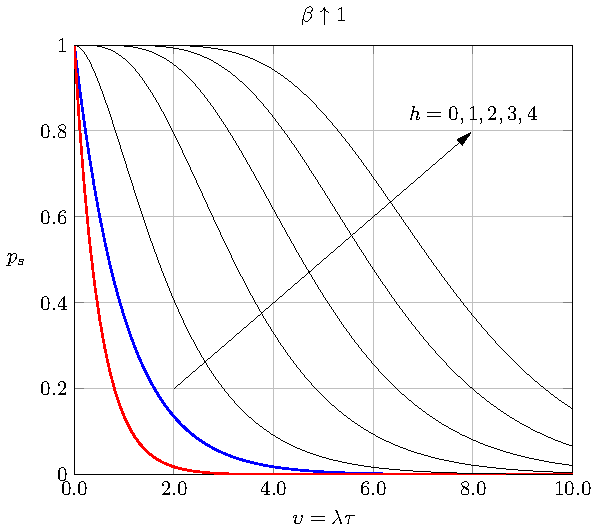
\includegraphics[width=\columnwidth]{Figures/Ch5_HI_1.pdf}
            % \caption{$\beta \uparrow 1$.}
        \label{fig:HI_1}
        \end{subfigure}
    \else
        
\includegraphics[draft, width=\textwidth]{Figures/placeholder.png}
    \fi
    \caption{Transmission success probability $p_s$ as a function of traffic $\upsilon$ in the HI model. The blue and red curves represent the slotted and unslotted ALOHA, respectively.} \label{fig:HI}
\end{figure}

As shown in the plots of Fig.~\ref{fig:HI}, the transmission success probability $p_s$ increases with $h$, because more concurrent interfering transmissions are necessary to cause \textit{high interference} in the typical packet transmission.

When we fix the threshold $h$ and let the traffic $\upsilon\to\infty$, we have that ${\P(\overline{S_h}=0)=0}$ and $\P(\overline{S_h}=1)=1$.
%
On the other hand, when we fix $\upsilon$ and let $h\to\infty$, then ${\P(\overline{S_h}=0)=1}$ and $\P(\overline{S_h}=1)=0$.
%
Thus, an interesting scenario to analyse is what happens when we increase the traffic $\upsilon$ along with the threshold $h$, i.e., let $\upsilon\to\infty$ and $h\to\infty$ such that $\frac{h}{\upsilon} \to 1$.
%
In this case we can show that
\begin{align*}
   \lim_{\substack{h,\upsilon\to\infty\\ h/\upsilon\to1}} \P(\overline{S_h} = 0) &=  \lim_{\substack{h,\upsilon\to\infty\\ h/\upsilon\to1}} \P(\overline{S_h} = 1) = \frac{1}{4}\left( 1 - \frac{2}{\pi}\right) \approx 0.091.
\end{align*}

\begin{note}
    To find the above result it is necessary to calculate an interesting limit problem, which cannot be solved through standard techniques, indeed the Software \textit{Mathematica} (version 12) does not solve it. In a simpler form, the problem is to show that
    \begin{align*}
        \lim_{n\to\infty} f_n(n) = \lim_{n\to\infty} \frac{\Gamma(n,n)}{\Gamma(n)} = \frac{1}{2},
    \end{align*}
    where $\Gamma(\cdot,\cdot)$ is the incomplete gamma function and is defined as $\Gamma(s,x)\triangleq \int_{x}^\infty t^{s-1} \euler^{-t}\,\d t$, and $\Gamma(\cdot) \triangleq \Gamma(\cdot,0)$ is the gamma function.
    
    To prove this identity we use the central limit theorem!
    
    Let $\{X_k\}_k$ be iid exponentially distributed random variables with parameter $1$. Let the sum $S_n = \sum_{k=1}^n X_k$, then $S_n$ follows an Erlang distribution of parameters $(n,1)$. Then, $\P(S_n > n) = \frac{\Gamma(n,n)}{\Gamma(n)}$. However, $\P(S_n > n) = \P(\frac{S_n-n}{\sqrt{n}} > 0) \xrightarrow{n\to\infty} 1/2$ by the central limit theorem.
\end{note}

To conclude this part, let us state the following inequalities, for $\beta > 0$, $\upsilon > 0$, $h\ge 0$,
\begin{align*}
    p_s^{\mathrm{(ALOHA)}} &\le p_s^{\mathrm{(ECC)}} \le p_s^{\mathrm{(AI)}} \le p_s^{\mathrm{(HI)}},\\
    \mathscr{T}^{\mathrm{(ALOHA)}} &\le \mathscr{T}^{\mathrm{(ECC)}} \le \mathscr{T}^{\mathrm{(AI)}} \le \mathscr{T}^{\mathrm{(HI)}},
\end{align*}
which are easily obtained from Remark~\ref{remark:Ch5_ineq} and the definitions of throughput and transmission success probability.

% % % % % % % % % % % % % % 
\section{Summary} \label{sec:summ_P2_01}

In this chapter, we characterized the distribution of the interference in a typical packet, where interferers transmit according to a Poisson process.
%
The characterization was performed through the analysis of some transmission success models (ECC, AI, HI), for which we obtained the throughput and the transmission success probability in closed form.
%
We also compared the obtained distributions with those of the slotted/unslotted ALOHA.


\chapter{Including Retransmission}
\label{cap:P2_02} \thispagestyle{empty}
\def\printfig{1} % Cap. 6
\chapterquote{%
Although modeling is a central component of modern science, scientific models at best are approximations of the objects and systems that they represent—they are not exact replicas. Thus, scientists constantly are working to improve and refine models.}
{-- Kara Rogers, \textit{Scientific modeling} (2011)}

In the previous chapter, there was no analysis regarding retransmission performance (e.g. delay) and related parameters (e.g. retransmission rate).
%
This is done in this chapter\footnote{The present chapter was based on the article \cite{dester2021retrans}.}.

Our main motivation for this part is to analyze the impact of limiting the maximum number of allowed retransmissions $m\in\N$ for each packet.
%
When we increase $m$, the throughput $\mathscr{T}$ increases because fewer packets are discarded. On the other hand, the delay $D$ also increases because the packet stays longer in the system and contributes to increasing the aggregate interference (see Remark~\ref{remark:optimization}).
%
Indeed, we prove that selecting the smallest number of allowed retransmissions that satisfy some requirements is the optimal approach.

Another problem that arises because we have a loss system is that the delay metric ignores discarded packets.
%
Thus, an ``optimal'' solution may consider discarding some packets only because the associated delays are large. This would artificially decrease the mean packet delay.
%
That is why we will use the Age-of-Information (AoI) metric along with the delay.
%
This metric takes into account the time spent by dropped packets and is defined in the following section.

\begin{remark} \label{remark:optimization}
    Regarding the optimization of $m$, it is desirable to have a single metric that takes into account both $\mathscr{T}$ and $D$ in a meaningful way, however that is not an easy task.
    %
    Of course we could propose objective functions such as, for constant $w_0 > 0$,
    \begin{align*}
        \mathscr{T} - w_0\,D, \qquad \frac{\mathscr{T}}{D}, \qquad \mathscr{T} \euler^{-w_0\,D},
    \end{align*}
    or any bivariate function which monotonically increases with $\mathscr{T}$ and monotonically decreases with $D$. All these examples lead to a Pareto optimum\footnote{A Pareto optimum is a situation where no changes can be made that improves a metric without worsting off another.}, however they do not carry (\textit{a priori}) any physical interpretation.
    %
    To circumvent this choice dilemma, we optimize the delay $D$ and consider the throughput $\mathscr{T}$ as a constraint of the optimization.
    %
    Then, we do not have to worry about application specificities and we can tackle the problem in a more general form.
\end{remark}

% % % % % % % % % % % % % % % % % % % % % % % % 
% % % % % % % % % % % % % % % % % % % % % % % % 
\section{Age-of-Information metric}

For a given user, at time $t$, let $U(t)$ be the time the last received packet was generated. Then, the AoI metric is defined as $\Delta(t) \triangleq t-U(t)$ \cite{kaul2011minimizing, kaul2012real}.
%
Thus, it measures the delay to refresh the information on the receiver.

In this chapter, we use a related metric called \textit{Peak-Age-of-Information} (PAoI), which corresponds to the \textit{Age-of-Information} when a packet is successfully received.
%
The mean PAoI metric considers the time spent by dropped packets, which represents an important difference from the classical mean delay metric that may provide a misleading result when we have a high proportion of discarded packets.

In our model, we assume that the generation of packets is modelled as events that follow a Poisson process. Thus, discarding a packet too soon (small $m$) may have a high cost in the PAoI metric, because the node does not know when the next packet is coming.

For example, let us take the cases of no retransmissions ($m=0$), one allowed retransmission ($m=1$) and no limit for retransmissions ($m = \infty$). If there is a long wait between the arrival of packets with successful transmission, we may observe what is shown in Figure~\ref{fig:PAoI_examples}.
%
Without retransmissions, only the packets that arrive and are successfully transmitted contribute to decreasing the AoI. When we allow one retransmission, the packets that have success in the first retransmission also contribute, and so on.
%
Fig.~\ref{fig:PAoI_examples} illustrates why increasing $m$ decreases the mean PAoI in this case.
%
\begin{figure}[htb]
    \centering
    \if\printfig1
        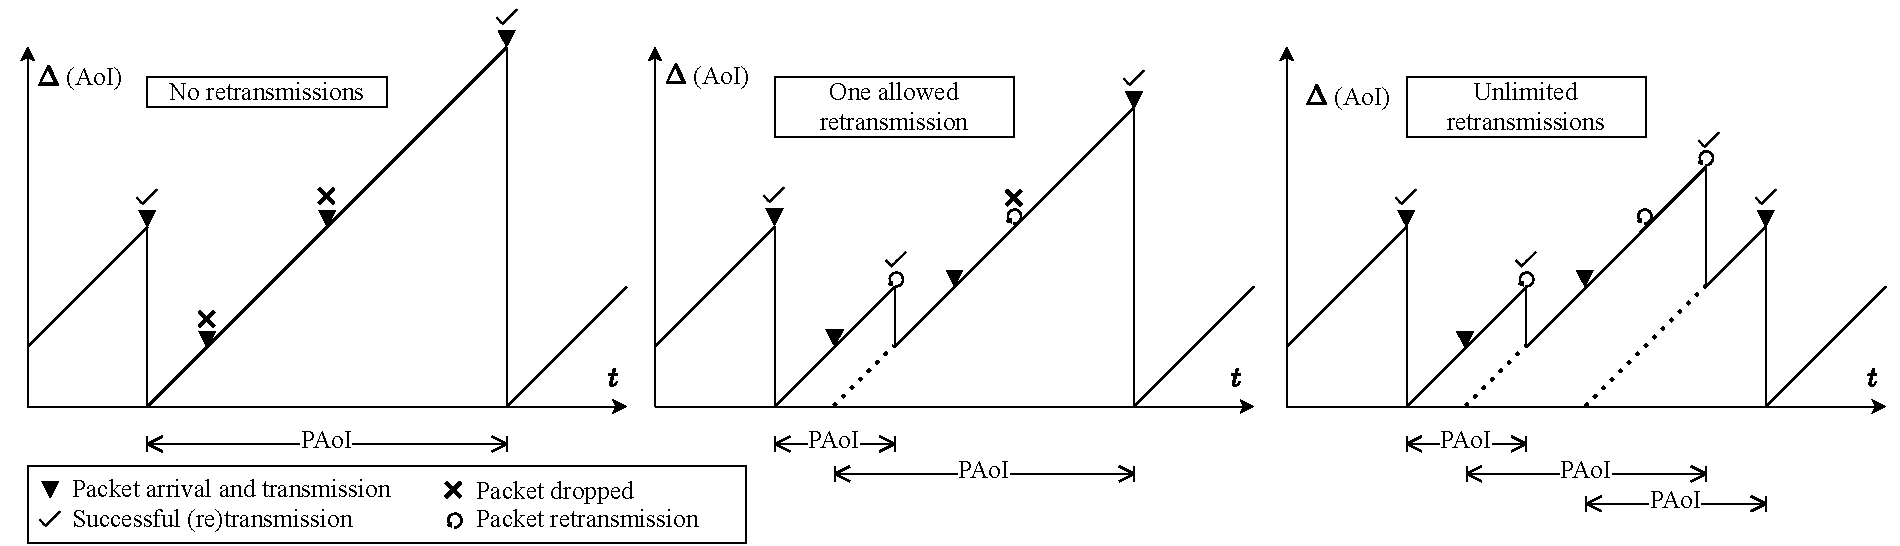
\includegraphics[width=\textwidth]{Figures/Ch6_PAoI_Intro.pdf}
    \else
        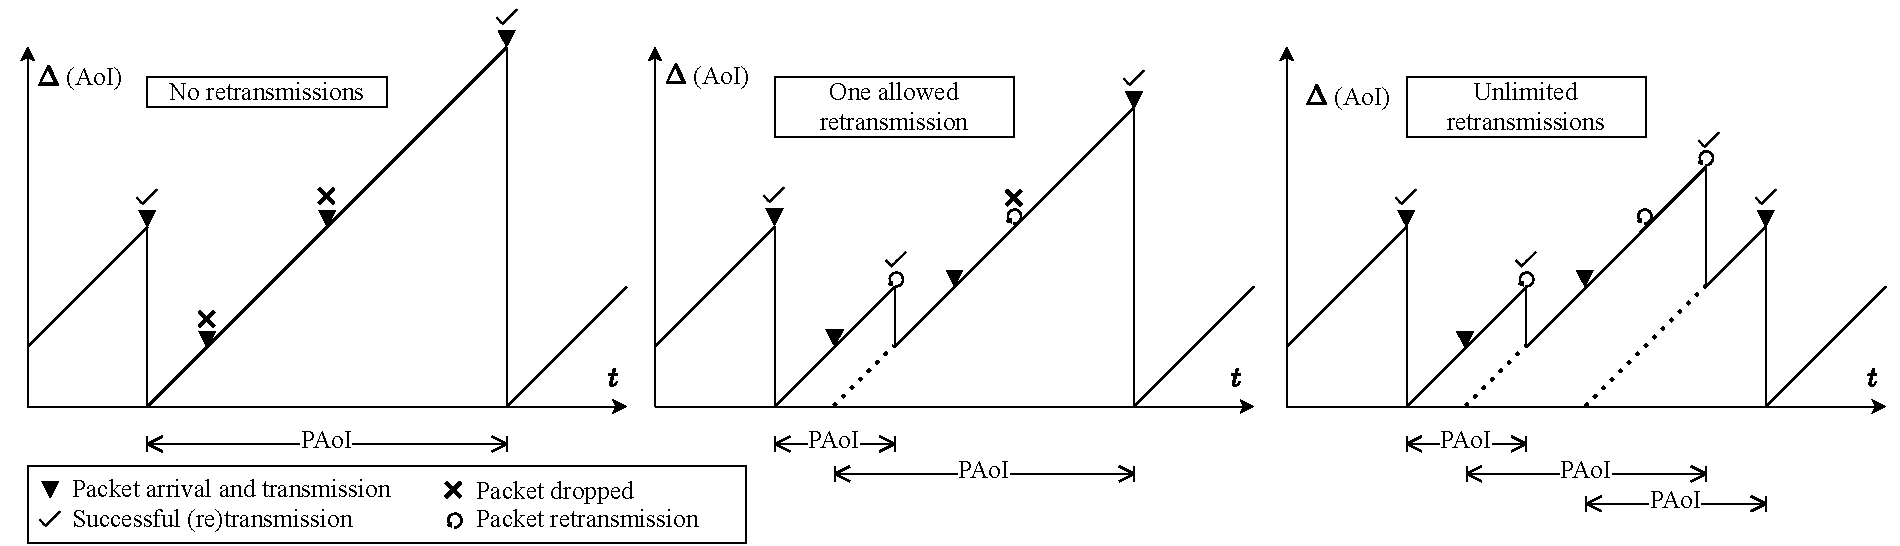
\includegraphics[width=\textwidth,draft]{Figures/Ch6_PAoI_Intro.pdf}
    \fi
    \caption{Examples of measures of the PAoI metric for different retransmission strategies.}
    \label{fig:PAoI_examples}
\end{figure}

On the other hand, if retransmissions are performed several times and a new packet arrives before a successful retransmission happens, then the old packet is dropped and the retransmissions only served to generate interference, thus increasing the PAoI.
%
% However, we cannot forget that increasing $m$ increases aggregate interference, which may increase the PAoI in the end.

% % % % % % % % % % % % % % % % % % % % % % % % 
% % % % % % % % % % % % % % % % % % % % % % % % 
\section{Random Access Network with Limited Retransmissions}

In this section, we analyze the impact of a limited number of retransmissions in the network performance by tuning the number of allowed retransmissions $m\in\N$ and the rate $r\in\R_+$ at which the packet to be retransmitted will access the network.
%
Specifically, we consider a scenario where only the most recent event matters, and thus, a packet waiting to be retransmitted is dropped whenever a new packet arrives.

Our aim in this work is to select the optimal pair $r$ and $m$ for the metrics throughput, delay, and PAoI.
%
The main differences of our work from recent works {\cite{chen2020age1, chen2020age2, yates2017status}} are that we deal with a general transmission success probability function of the traffic, i.e., this can represent the collision model, the capture model, or any arbitrary model that does not depend directly on $r$ and $m$. Also, we consider limiting the maximum number of retransmissions to improve performance.
%
In this framework, we prove that selecting the smallest number of allowed retransmissions that satisfy some requirements is the optimal approach.

% In {\cite{chen2020age1, chen2020age2, yates2017status}}  {the transmission success probability is derived from the classical collision model;}
% %
% in \cite{chen2020age1}  {the authors propose a random access scheme to optimize the AoI for a set of arrival rates and a large number of nodes;}
% %
% in {\cite{chen2020age2}}  {the authors propose a random access scheme to optimize the AoI based on the instantaneous AoI of each node;}
% %
% in {\cite{yates2017status}}  {the authors show that random access perform worse than scheduled access with feedback by a factor of approximately $2\euler$ in the AoI.}

%-%-%-%-%-%-%-%-%-%-%-%-%-%-%-%-
\subsection{System Model}

Consider a single class stationary and ergodic network with a given number of nodes (possibly infinite), each node receives a packet whenever an event associated with that node occurs, and we suppose the events occur according to a Poisson process of parameter $a > 0$.
%
Thus, $a$ is also the arrival rate of packets per node. Once the packet arrives, the node transmits the packet\footnote{{This assumption can be easily modified to transmit the packet after an exponentially distributed time upon arrival without compromising the analytical tractability.}} to a receiver. If the packet is successfully transmitted, it is dropped\footnote{Successful reception acknowledgment is transmitted in an error-free channel.}.
%
Otherwise, the node transmits it again after an exponentially distributed time with a parameter $r > 0$, which is the retransmission rate.

In this scenario, we suppose that only the data related to the most recent event matter, i.e.,
% if a new packet arrives while the node is still trying to retransmit an older packet, then the latter is dropped and the new packet is transmitted.
if a new packet arrives, the old one waiting to be retransmitted is dropped. Another case where the packet is also dropped is when it reaches the number of allowed retransmissions $m \in \Z_+$.
%
To attain analytical tractability of the system model we further assume:
%
\begin{itemize}[itemsep=3pt,parsep=3pt,topsep=3pt,partopsep=3pt]
    \item stationary homogeneous traffic $\upsilon$ per unit of area, i.e., all receivers experience interference with the same distribution\footnote{
     {The main purpose of this assumption is to eliminate the intricate coupling and interactions between the transmitting nodes.}
    %
    This is valid in large-scale networks with high-mobility nodes, or with a small access probability \cite{haenggi2013diversity}, or with frequency hopping in several channels.};
    % \item the interference process is iid for each transmission\footnote{This is a valid assumption in high-mobility systems \cite{baccelli2010stochastic} or if there is frequency hopping in a sufficiently large number of channels \textcolor{red}{[Referência]}};
    \item transmission time is negligible compared with the waiting time to retransmit or for a new packet to arrive in the node;
    \item stationary success probability of a single transmission is a general function $p_s:\R_+\longrightarrow[0,1]$ of traffic $\upsilon$ that satisfies the conditions of Theorem~\ref{th:unique_opt}, which guarantees existence and uniqueness of the optimum throughput.
\end{itemize}

The first assumption along with having a single user class entail that the system throughput is a function of the traffic $\upsilon$ and it is given by $\mathscr{T}(\upsilon) = \upsilon\,p_s(\upsilon)$.

\begin{figure}[htb]
    \centering
    \if\printfig1
        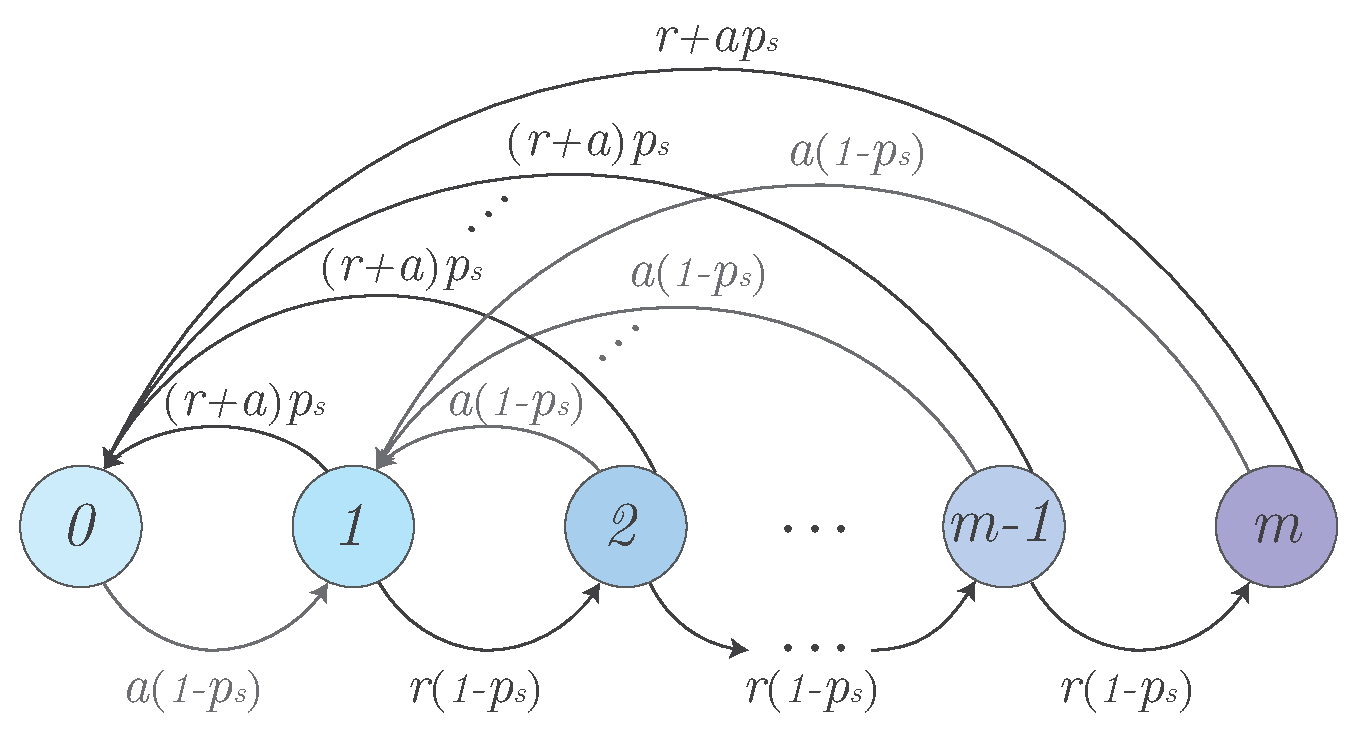
\includegraphics[width=0.6\textwidth]{Figures/Ch6_markch.pdf}
      %\includegraphics[width=\columnwidth]{images/markovDiagram.pdf}
    \else
        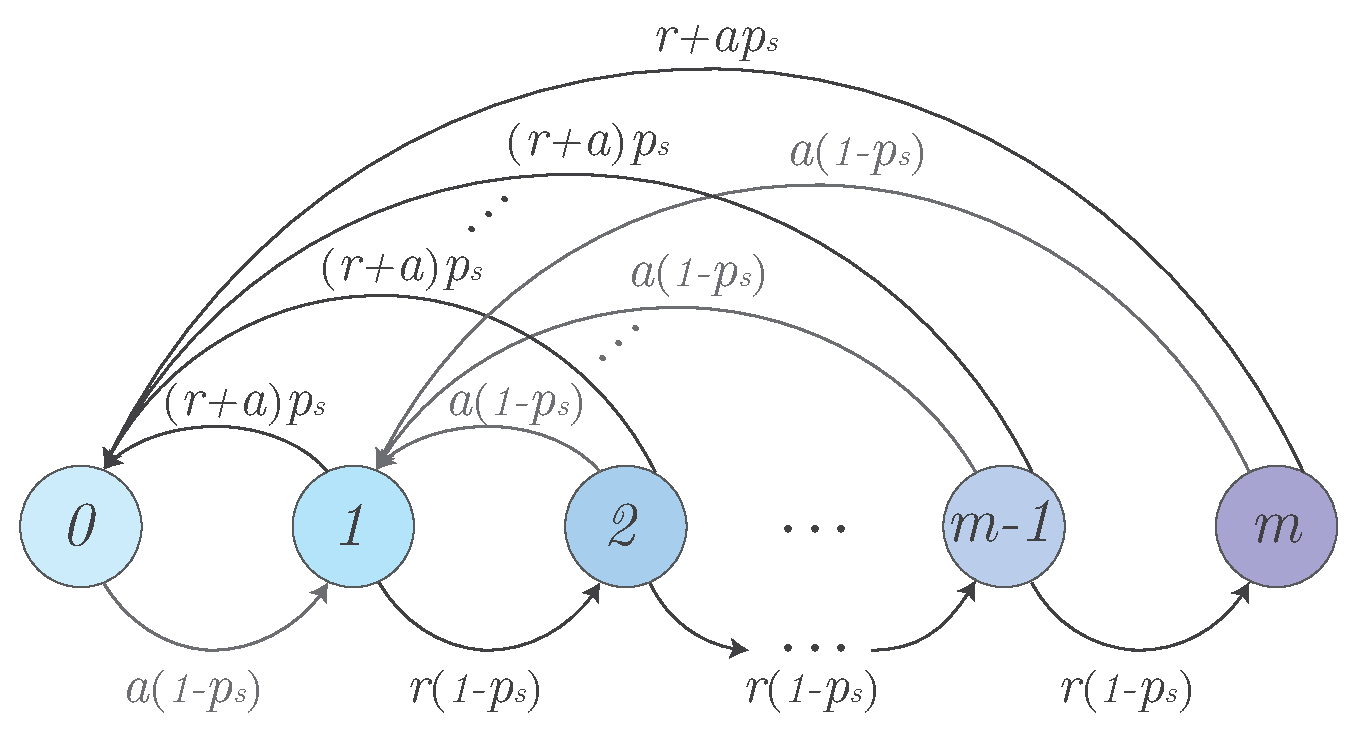
\includegraphics[draft,width=0.6\textwidth]{Figures/Ch6_markch.pdf}
    \fi
    \caption{Markov chain transition rates for a typical node.}
    \label{fig:markov_diagram}
\end{figure}

From now on, let us use $p_s$ to denote $p_s(\upsilon)$ to lighten the notation.

The state of a typical node can be represented as a continuous-time Markov chain with transition rates (Definition~\ref{def:transition-rate}):
\begin{align*}
    k \to k+1:&~ r\,(1-p_s), && 0 < k < m, \\
    k \to 1:&~ a\,(1-p_s),   && 0 \le k \le m, \\
    k \to 0:&~ (r + a)\,p_s, && 0 < k < m, \\
    m \to 0:&~ r + a\,p_s,
    % \text{otherwise}:&~ 0,
\end{align*}%
 {where the state $k\in\{1,2,\dots,m\}$ represents the number of transmissions that occurred with the buffered packet, and $k=0$ represents that the buffer is empty.}
%
These transition rates are illustrated in the diagram of Fig.~\ref{fig:markov_diagram}.
%, where $a$ is the arrival rate of new packets per node, $r$ is the rate of retransmission packets, $p_s$ is the packet success probability.
The nodes that are retransmitting have a transmission rate of $r+a$ because they can transmit either by retransmission or when a new packet arrives.
%
The nodes that are not retransmitting ($k=0$) have a transmission rate of $a$.

More specifically,
%
the transition $k\to k+1$ represents an unsuccessful retransmission (with probability $1-p_s$), which occurs at rate $r$;
%
the transition $k\to 1$ represents an unsuccessful transmission (with probability $1-p_s$) of an arriving packet, which occurs at rate $a$;
%
the transition $k\to 0$ corresponds to a successful transmission (with probability $p_s$), which can be from a retransmitted packet (rate $r$) or arriving packet (rate $a$);
%
finally, the transition $m\to 0$ corresponds to a successful or unsuccessful transmission, because in this state ($m$ retransmissions) the packet is dropped even with failure.

In view of the general network model of Chapter~\ref{cap:P2_00} we provide a possible example of a network that fits the above assumptions.
%
\begin{example} 
    Consider a stationary and ergodic high-mobility bipolar Poisson network with one user class and density of transmitters $\lambda_{\S}>0$ on the plane $\S=\R^2$, transmission time $\tau_i = \tau$ and transmission power $P_i \equiv 1$ for every user $i\in\N$, and link distance $r_0 > 0$.
    
    For each transmitter $i\in\N$, suppose packets arrive according to a Poisson point process $A_i$ of density $a>0$ on time $\T = \R$. Each transmitter can access the channel according to a Poisson point process $U_{i}$ of density $r>0$ or if a packet arrived. Thus, transmissions can happen according to the point process $T_i = A_i + U_i$. However, they only happen if there is a packet in the buffer, thus transmissions will happen according to the thinned point process $T^*_{i} = q_i\,T_i$, where the function $q_i = \ind\{Q_i(t) > 0\}$, and the queue dynamics of $Q_i$ is defined such that it follows the continuous-time Markov process presented in Figure~\ref{fig:markov_diagram}.
    
    Furthermore, assuming Rayleigh fading, path loss function $\ell(x) = x^{-\alpha}$, $\alpha>2$, and the \textit{capture model} with threshold $\theta>0$ for the transmission success probability, then according to Theorem~\ref{prop:PPP_ps} we have that
    \begin{align*}
        p_s = \exp\!\left( -\upsilon \pi r_0^2 \theta^\delta \frac{\delta\pi}{\tau\sin(\delta\pi)} \right),
    \end{align*}
    where $\delta\triangleq 2/\alpha$.
    
    Thus, $p_s$ essentially depends on the traffic $\upsilon$ and other constants. Therefore, the system model presented in this section applies to this network.
\end{example}

Let us define $\{\pi_k\}_{k\in\Z_+}$ as the stationary probabilities of the typical node being in the $k$th retransmission.
%
Then, in the stationary state, the network traffic is given by%
\begin{align} \label{eq:traffic_ret}
    \upsilon &= \frac{\upsilon_0}{a} \left( a \pi_0 + (r+a) (1-\pi_0) \right) = \upsilon_0 \left( 1 + \frac{r}{a} (1 - \pi_0) \right),
\end{align}
where $\upsilon_0$ is the traffic without retransmission, i.e., if $r=0$, then $\upsilon=\upsilon_0$.
%
It is important to remember that $p_s$ depends on the traffic of the system, and thus, we have a challenging problem because $\upsilon$ also depends on $p_s$ owing to the dependence on the stationary probabilities. % See Proposition~\ref{prop:pi} in the following section.
The following section circumvents this problem and presents the analytical results.

%-%-%-%-%-%-%-%-%-%-%-%-%-%-%-%-
\subsection{Analysis}

Let us assume that the packet arrival rate $a$ and the traffic without retransmissions $\upsilon_0$ are fixed and known.
%
Our objective here is to optimize the retransmission rate $r$ and the number of allowed retransmissions $m$ in view of some performance metrics.
%
We begin by solving the Markov chain of Fig.~\ref{fig:markov_diagram} for its stationary probabilities.
%
The following proposition gives us the stationary probabilities (Definition~\ref{def:markov-defs}) of the Markov chain.

\begin{proposition} \label{prop:pi}
    The stationary probability $\pi_k$ of finding the typical node in the $k$th retransmission state is given by
    \begin{align*}
        % \pi_0 &= 1 - \frac{a}{r}\,\frac{1-p_s}{p_s +a/r}\left(1-\left(\frac{1-p_s}{1+a/r}\right)^m\right),\\
        \pi_0 &= 1 - \frac{a}{r} \frac{\xi\,(1-\xi^m)}{1-\xi},\\
        \pi_k &= \frac{a}{r}\,\xi^k, \qquad 1\le k\le m,
    \end{align*}
    where $\xi \triangleq \dfrac{r(1-p_s)}{r+a}$ is the retransmission probability.
\end{proposition}

\begin{proof}
    From the Markov chain transition probabilities, we have that, for $2\le k\le m$,
    $
        (r+a)\pi_k = r (1-p_s) \pi_{k-1}.
    $
    Thus, $\pi_k = \left(\frac{r(1-p_s)}{r+a}\right)^{k-1}\pi_1$.
    Using this relation along with
    \begin{align*}
        a(1-p_s)\pi_0 &= (r+a)p_s\sum_{k=1}^m\pi_k + r(1-p_s) \pi_m,\\
        r(1-p_s)\pi_1 &= (r p_s+a)\sum_{k=2}^m\pi_k + r(1-p_s) \pi_m,
    \end{align*}
    and $\sum_{k=0}^m \pi_k = 1$, we find the desired solution.
\end{proof}

Using Proposition~\ref{prop:pi}, we can rewrite \eqref{eq:traffic_ret} in the simpler form
\begin{align} \label{eq:traffic_ret2}
    \upsilon = \frac{1-\xi^{m+1}}{1-\xi} \upsilon_0.
\end{align}

Let $\upsilon^*\in\R_+$ be the traffic for which we have the maximum throughput $\mathscr{T}^* = \upsilon^* p_s^*$, where $p_s^* = p_s(\upsilon^*)$. Theorem~\ref{th:unique_opt} guarantees the existence and uniqueness of $\upsilon^*$.
%
The optimum traffic $\upsilon^*$ can be found by solving the equation $\psi(\upsilon^*) = 1$, where $\psi$ is defined in Theorem~\ref{th:unique_opt}.
%
We can achieve $\upsilon^*$ by adjusting the retransmission rate to an appropriate $r^*$ for each $m\in\Z_+$.

When $m=1$,\vspace{-5mm}
\begin{align}
    r^* = \frac{a(\upsilon^*-\upsilon_0)}{(2-p_s^*)\upsilon_0 - \upsilon^*}, \quad\text{if}~ \frac{\upsilon^*}{2-p_s^*} < \upsilon_0 \le \upsilon^*.
\end{align}

When $m = \infty$, i.e., unlimited number of retransmissions,
\begin{align} \label{eq:opt_retr_rate}
    r^* = \frac{a\,(\upsilon^*-\upsilon_0)}{\upsilon_0 - p_s^* \upsilon^*}, \quad\text{if}~ p_s^* \upsilon^* < \upsilon_0 \le \upsilon^*.
\end{align}

As expected, the inequality on $\upsilon_0$ when $m=1$ is more strict than for $m = \infty$, since we can achieve greater traffic with the latter.
%
For general $m\in\N$, we have the following result.

\begin{lemma} \label{lem:max_lam}
    For all $r\in\R_+$, $m\in\N$,
    % \begin{align*}
    %     \frac{\upsilon}{\upsilon_0}
    %         = \frac{1-(1-p_s)^{m+1}}{p_s}.
    % \end{align*}
    \begin{align*}
        1 \le \frac{\upsilon}{\upsilon_0} \le \frac{1-(1-p_s)^{m+1}}{p_s}.
    \end{align*}
\end{lemma}
%
\begin{proof}
    First, let us prove that for a fixed $p_s$, we have 
    $
        {\frac{\partial \upsilon}{\partial r} \ge 0}.
    $
    \begin{align*}
        \frac{\partial \upsilon}{\partial r} = \upsilon_0\, \frac{a/r}{a+r}\, \frac{\beta^{m+1} - m(\beta-1)-\beta}{\beta^m (\beta-1)^2},
    \end{align*}
    where $\beta\triangleq \xi^{-1} \ge 1$. Notice that the expression
    \begin{align*}
        \beta^{m+1} - m(\beta-1)-\beta &= (1+(\beta-1))^{m+1} - (m+1)(\beta-1) - 1 \\
            &= \left(\sum_{k=0}^{m+1} \binom{m+1}{k} (\beta-1)^k\right)- (m+1)(\beta-1) - 1\\
            &= \sum_{k=2}^{m+1} \binom{m+1}{k} (\beta-1)^k \\ &\ge 0.
    \end{align*}
    Therefore,
    $
        {\frac{\partial \upsilon}{\partial r}\ge 0}.
    $
    Then, $\displaystyle \upsilon_0 \le \upsilon \le \lim_{r\to\infty} \upsilon$, from which we conclude the proof through the calculation of the limit.
\end{proof}

A consequence of Lemma~\ref{lem:max_lam} is that to achieve the optimum traffic $\upsilon^*$ we must have
\begin{align} \label{eq:opt_cond}
    \frac{p_s^*\upsilon^*}{1-(1-p_s^*)^{m+1}} < \upsilon_0 \le \upsilon^*.
\end{align}

There might exist several values for $m$ that satisfy \eqref{eq:opt_cond}.
%
Let us focus on the optimal choice in view of some performance metrics.

% % % % % % % % % % % % % % % % % % % % % 
\subsubsection{Stationary Mean Delay}

% The throughput $\mathscr{T} = \upsilon\,p_s$ can also be calculated as the product of the traffic without retransmissions $\upsilon_0$ and the probability that a packet is not dropped, i.e., $\mathscr{T} = \upsilon_0 \, \P(D < \infty)$, where 
Let $D$ be the \textit{improper} random variable that represents the delay of a typical packet. If it is dropped, then ${D=\infty}$.
%
From the Markov chain and the fact that the sum of exponential iid random variables follows an Erlang distribution, we can show that the cdf of $D$ is
\begin{align*}
    F_D(t) = p_s + \int_0^t f_D(t)\,\d t, \qquad 0\le t < \infty,
\end{align*}
where
\begin{align}
    f_D(t) = \sum_{k=1}^m p_s\,\xi^k \frac{ (r+a)^k t^{k-1}}{(k-1)!} \,\euler^{-(r+a) t}, \qquad t\in\R_+.
        % &= p_s\delta_0(t) + p_s \xi\,(r+a) \frac{\Gamma\left(m, \xi\,(r+a) t\right)}{\Gamma(m)}\,\euler^{-(1-\xi) (r+a) t}, \nonumber
\end{align}

\begin{note}
    Note that the rate associated with the Erlang distribution to calculate the function $f_D$ is the sum of the rate of retransmission $r$ with the rate of arrival $a$ instead of simply $r$.
    %
    This might be counter-intuitive because we are conditioning on the event of retransmitting the packet to calculate the delay.
    %
    This is associated with the following interesting problem.
    
    Let $X, Y$ be independent random variables that follow exponential distributions of parameters $\alpha$ and $\beta$, respectively.
    %
    Let $0 < \alpha < \beta$, $t\in\R_+$. We invite the reader to compare, without calculations, the probabilities $\P(\min(X,Y)\le t)$ and $\P(\min(X,Y)\le t \mid X \le Y)$.

    For independent $X\sim\mathscr{E}(\alpha)$ and $Y\sim\mathscr{E}(\beta)$, standard calculations show the possibly counter-intuitive result
    $\P(\min(X,Y)\le t) = 1 - \euler^{-(\alpha+\beta)t} = \P(\min(X,Y)\le t \mid X \le Y).$
    
    That is, $\min(X,Y) \sim \mathscr{E}(\alpha+\beta)$ and $\min(X,Y) \mid X \le Y \sim \mathscr{E}(\alpha+\beta)$.
    %
    We say counter-intuitive because we could, for example, expect that $\min(X,Y) \mid X \le Y \sim \mathscr{E}(\alpha)$.

    % \begin{align*}
    %     \P(\min(X,Y)\le t)
    %         &= 1 - \P(\min(X,Y) > t) \\
    %         &= 1 - \P(X > t, Y > t) \\
    %         &= 1 - \P(X > t)\,\P(Y > t) \\
    %         &= 1 - \euler^{-(a+b)t}.
    % \end{align*}
    
    % \begin{align*}
    %     \P(\min(X,Y)\le t \mid X \le Y)
    %         &= \frac{\P(\min(X,Y)\le t, X \le Y)}{\P(X \le Y)} \\
    %         &= \frac{\P(X \le t, X \le Y)}{\P(X \le Y)}\\
    %         &= \dfrac{\displaystyle \int_0^t f_X(x) \left( \int_x^\infty f_Y(y) \d y \right) \d x}{\displaystyle \int_0^\infty f_X(x) \left( \int_x^\infty f_Y(y) \d y \right) \d x} \\
    %         &= 1 - \euler^{-(a+b)t}.
    % \end{align*}
    
    In our original problem, this means that conditioning on the event of having retransmission does not reduce the rate to $r$, i.e., it continues to be the sum of the retransmission and the arrival rates $r+a$.
\end{note}

\begin{note}
    Note that $f_D$ is not the pdf of $D$. The pdf does not exist (with respect to the Lebesgue measure) as discussed in Note~\ref{note:dirac_function}, because the events $\{D=0\}$ and $\{D=\infty\}$ have positive probability measures.
\end{note}

The event of packet success is equivalent to $D<\infty$, thus the packet success probability
%
\begin{align} \label{eq:pps}
    p_p = \P(D<\infty) = p_s\frac{1-\xi^{m+1}}{1-\xi}.
\end{align}
%
As expected, this satisfies $\upsilon_0 p_p = \upsilon p_s = \mathscr{T}$. %, because it is another form of calculating the throughput.

Then, the mean delay of a successfully transmitted packet, which we shall define as
\begin{align} \label{eq:delay}
    \overline{D} \triangleq \E[D\mid D<\infty] &= \frac{\int_0^\infty t\, f_D(t)\, \d t}{\P(D<\infty)} 
        % &\quad = \frac{1-p_s}{p_s r+a}
        % \left( \frac{1 - \left(1 + m\frac{p_s+a/r}{1+a/r}\right) \left(\frac{1-p_s}{1+a/r}\right)^m}{1 -  \left(\frac{1-p_s}{1+a/r}\right)^{m+1} } \right).
        = \frac{1}{r+a}\left(\frac{1}{1-\xi} - \frac{1+m\xi^{m+1}}{1-\xi^{m+1}}\right).
\end{align}

% % % % % % % % % % % % % % % % % % % % % 
\subsubsection{Stationary Mean PAoI}
%
\begin{figure}[htb]
    \centering
    \if\printfig1
        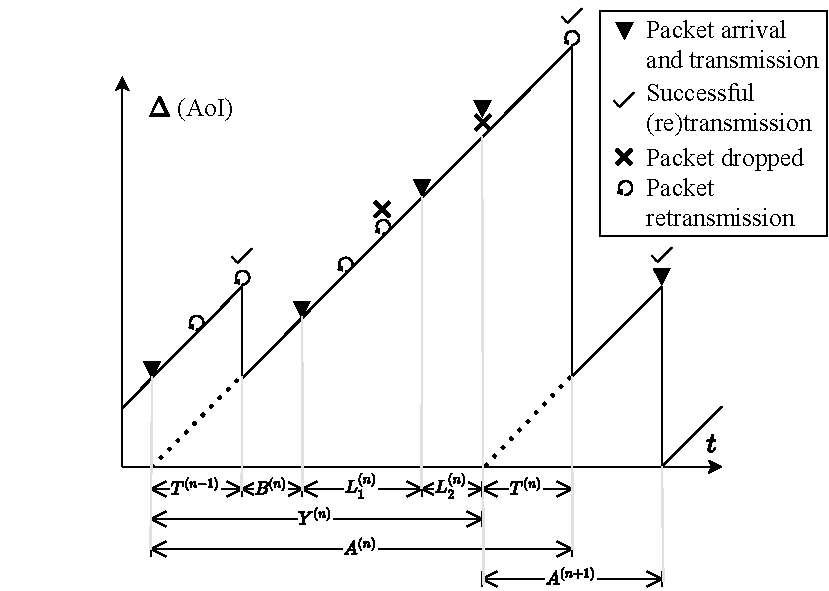
\includegraphics[width=0.7\columnwidth]{Figures/Ch6_PacketRetransmission_PAoI.pdf}
    \else
        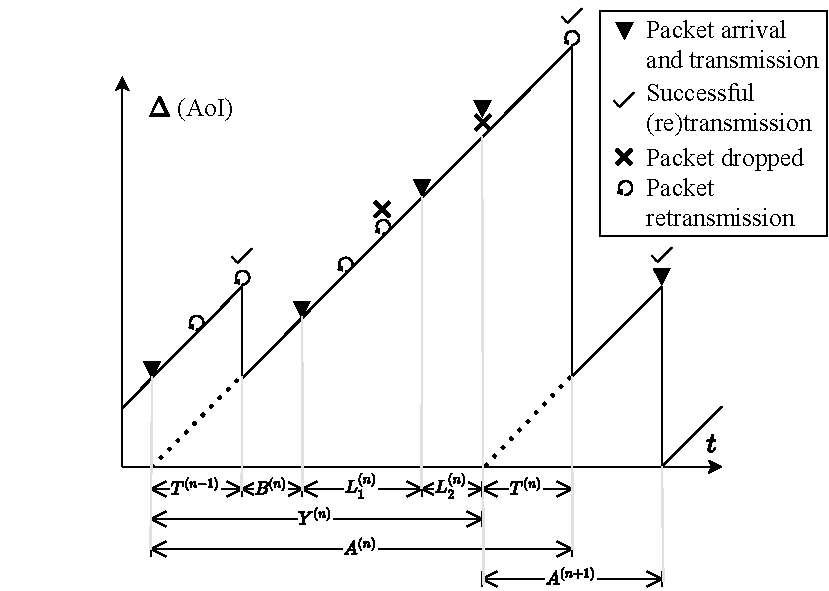
\includegraphics[draft,width=0.85\columnwidth]{Figures/Ch6_PacketRetransmission_PAoI.pdf}
    \fi
    \caption{Time evolution of the \textit{Age-of-Information} metric. The \textit{Peak-Age-of-Information} $A^{(n)}$ is the measure of the \textit{Age-of-Information} when a packet is successfully transmitted. In this example, the first dropped packet is due to reaching the maximum number of retransmissions ($m=2$) and the second dropped packet is due to the arrival of a new packet.
    %
    Except for the discontinuities, note that the AoI is always increasing with slope $1$, because it measures the time since the generation of the last correctly received packet.
    %
    Also note that $Y^{(n)}$ comprises the time between the arrival of packets that are successfully transmitted, i.e., the first and the fourth packet in this case.
    }
    \label{fig:PAoI_diagram}
\end{figure}

The random variable PAoI $A^{(n)}$ measures the time between the $n$th successfully received packet transmission and the previous successfully received packet generation. It is defined as
\begin{align}\label{eq:A}
    A^{(n)} = Y^{(n)}+T^{(n)},
\end{align}
where $Y^{(n)}$ is the interarrival time between packets of a typical node that are not dropped, and $T^{(n)}$ is the time a packet that is not dropped spends in the system, i.e., $\E[T^{(n)}] = \overline{D}$.

Fig.~\ref{fig:PAoI_diagram} shows a realization of the stochastic process with $m=2$ and two dropped packets.
%
% whenever it applies for all $n$. The random variable $Y$ is composed of the time spent with a successfully transmitted packet plus a packet arrival, as illustrated in Fig.~\ref{fig:PAoI_diagram}, which shows a realization of the stochastic process with $m=2$ and two dropped packets. Then,
The random variable $Y^{(n)}$ is composed by
\begin{align}\label{eq:Y}
    Y^{(n)} = T^{(n-1)} + B^{(n)} + \sum_{i=1}^{K^{(n)}} L^{(n)}_i,%
\end{align}%
where $B\sim\mathscr{E}(a)$ %follows an exponential distribution of the parameter $a$ and 
represents the packet arrival time since the last successful transmission (memoryless property),
%
$K\sim\mathscr{G}(p_p)$ %follows a geometric distribution of parameter $p_p$ and
represents the number of dropped packets until the arrival of a packet that is not dropped,
%
and $L_i$ is the time spent by the $i$th dropped packet since its arrival until a new packet arrives, its distribution is decribed in the proof of Proposition~\ref{prop:meanPAoI}. % which is independent from $T$ and $\{L_i\}_i$.
%
% A realization of the stochastic process, where we have $m=2$ and two dropped packets, is shown in Fig.~\ref{fig:PAoI_diagram}.

A closed-form expression for the mean PAoI metric is given by the following proposition.

\begin{proposition}\label{prop:meanPAoI}
    The stationary mean PAoI is given by
    \begin{align} \label{eq:PAoI}
        \E[A] &= \frac{1}{a}\!+\!\frac{1}{a+r} \frac{1-\xi^m}{1-\xi^{m+1}}
            \left( \frac{1-p_s}{p_s} + \frac{\xi}{1-\xi} - \frac{m\xi^{m+1}}{1-\xi^m} \right)\nonumber\\
            &\quad + \frac{1}{a}(1-p_s)\,\xi^m\left(\frac{1-\xi}{p_s\,(1-\xi^{m+1})}-1\right).
    \end{align}
    %
    Also,\qquad\qquad
    $\displaystyle
        \lim_{m\to\infty}\E[A] = \frac{1}{a} + \frac{1}{a+r}\left(\frac{1-p_s}{p_s} + \frac{\xi}{1-\xi}\right).
    $
\end{proposition}
\begin{proof}
    Using the Markov chain we can show that the moment generating function of $L$ and its expectation is given by
    
    \begin{align}
        M_L(t) &= \E[\euler^{-t L}] \nonumber\\
            &= \frac{1}{\P(D\!=\!\infty)} \bigg( \sum_{k=1}^m (1-p_s-\xi)\xi^{k-1} \left( 1 - \frac{t}{r+a} \right)^{-k} \nonumber\\
            &\qquad + (1-p_s) \xi^m \left( 1 - \frac{t}{r+a} \right)^{-m}\left( 1 - \frac{t}{a} \right)^{-1} \bigg),\nonumber\\
        \E[L] &= \left. \frac{\d}{\d t} M_L(t) \right|_{t=0} \label{eq:EL} \nonumber\\ 
            %\frac{1 - p_s - \xi - \xi^m (p_s (m (\xi -1) \xi -1)-\xi +1)}        {(r+a)(1 -\xi)\left(1-\xi-p_s(1-\xi^{m+1})\right)}\nonumber\\
            &= \frac{1}{r+a}\left( \frac{1}{1-\xi} - \frac{\xi^m(1-p_s(1+m\xi))}{1-\xi-p_s(1-\xi^{m+1})} \right) + \frac{1}{a}(1-p_s)\xi^m.
    \end{align}
    %
    % Also,
    % \begin{align*}
    %     \lim_{m\to\infty} \E[L] = \frac{1}{(r+a)(1-\xi)}.
    % \end{align*}
    % It is possible to find a closed form for the distribution of $Y$ (for example, through generating functions), however the final expression is so cumbersome that it will not help in any way.
    
    Using \eqref{eq:A}, \eqref{eq:Y} and taking the expectation gives us
    \begin{align*}
        \E[A] 
            = \E[Y] + \E[T]
            % &= \E[B] + 2\,\E[T] + \sum_{k=0}^\infty p_p \P(D=\infty)^k k\,\E[L] \\
            = a^{-1} + 2\,\overline{D} + \E[K] \E[L].
    \end{align*}
    % This metric takes into account not only the mean delay of a successful packet, but the total delay in updating the information caused by the unsuccessful packets as well.
    % %
    % Indeed, this metric is objectively more demanding than the mean delay, since the expected number of dropped packets between successful transmissions $\E[K]$ decreases with $m$.
    
    Then, using \eqref{eq:pps}, \eqref{eq:delay}, and \eqref{eq:EL} concludes the proof.
\end{proof}

% % % % % % % % % % % % % % % % % % % % % 
\subsubsection{Retransmission Optimization}
Finally, we can state the main result of the present chapter.%
\begin{proposition} \label{prop:best_m}
    Let $\upsilon\in\R_+$. If $\upsilon_0 \in (\upsilon p_s(\upsilon), \upsilon)$,
    then there exist infinite pairs of retransmission rates $r\in\R_+$ and number of allowed retransmissions $m\in\Z_+$ that achieve the network traffic $\upsilon$. Furthermore, the pair with the smallest $m$ has the minimal mean delay $\overline{D}$ and mean PAoI $\E[A]$.
\end{proposition}
%
\begin{proof}
    If $p_s \upsilon < \upsilon_0 < \upsilon$, then there exist an infinite number of pairs $m,r$ that we can choose to reach the desired traffic $\upsilon$, because for each integer $m$ that satisfies Lemma~\ref{lem:max_lam} there exists a unique $r\in\R_+$ that achieves the traffic $\upsilon$, by the fact that $\partial\upsilon/\partial r > 0$ from the proof of Lemma~\ref{lem:max_lam}.
    
    After some tedious manipulations using the definition of $\xi$ along with \eqref{eq:traffic_ret2}, we can rewrite \eqref{eq:delay} and \eqref{eq:PAoI} as
    \begin{align*}
        \overline D &= \frac{1-p_s-\xi}{ a\,(1-p_s)(1-\xi)} \left( \xi - (\Upsilon+\xi-1) \frac{\ln\!\left(\frac{\Upsilon}{\Upsilon+\xi-1}\right)}{\ln(1/\xi)} \right),\\
        \E[A] &= \frac{1}{a}\Bigg[ 1 + (\Upsilon-p_s)\frac{1-p_s}{p_s} \frac{\Upsilon+\xi-1}{\xi\Upsilon} + \frac{1-p_s-\xi}{\xi\,(1-p_s)} (1-\Upsilon) \times\\
            &\qquad\qquad \left(\frac{1-p_s}{p_s} + \frac{\xi}{1-\xi}
              - \frac{\xi\,(\Upsilon+\xi-1) \ln\!\left(\frac{\xi\Upsilon}{\Upsilon+\xi-1}\right)}{(1-\xi)(1-\Upsilon)\ln(1/\xi)} \right) \Bigg],
    \end{align*}
    where $\Upsilon \triangleq \upsilon_0/\upsilon$ is fixed. Further, from Lemma~\ref{lem:max_lam} we can state that $0 \le 1-\Upsilon \le \xi \le 1-p_s \le 1$.
    %
    Then, we can show that $\frac{\partial \overline D}{\partial \xi} \le 0$ and $\frac{\partial \E[A]}{\partial \xi} \le 0$ as $\xi\in(1-\Upsilon,1-p_s)$.
    %
    We know that $m$ decreases with $\xi$ for a fixed $\Upsilon$ (see \eqref{eq:traffic_ret2}), then to achieve the smallest mean delay and mean PAoI, we must use the smallest $m$. This concludes the proof.
\end{proof}

% Minimizing the PAoI is harder than minimizing the delay, in the sense that the PAoI takes into account the time spent by unsuccessful packets until a successful transmission occurs, i.e., it is a more demanding version of the mean delay metric, which only takes into account the time spent by successful packets and might not be ideal as a performance measure of a network with a high packet dropping rate.

Given a requirement (constraint) among the metrics throughput $\mathscr{T}$, network traffic $\upsilon$, and packet success probability ${p_p}$, we should use the smallest number of allowed retransmissions $m$ such that we can adjust the retransmission rate $r$ to achieve the requirement and satisfy Lemma~\ref{lem:max_lam}.
%
Then, according to Proposition~\ref{prop:best_m}, we minimize both the metrics mean delay $\overline{D}$ and mean PAoI $\E[A]$.

\begin{figure}[htb]
\centering
    \begin{subfigure}[t]{.45\textwidth}
      \centering
        \if\printfig1
            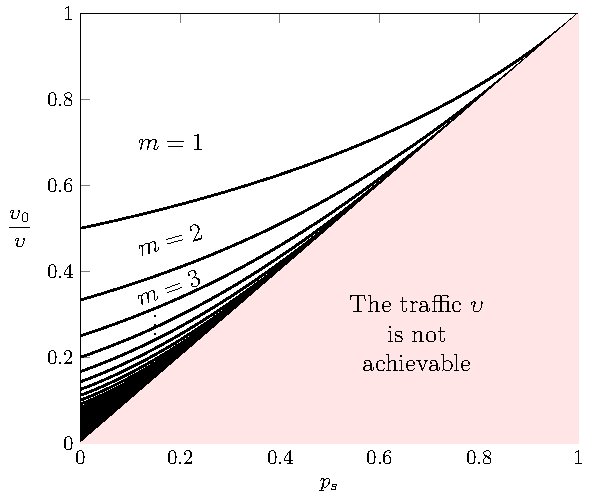
\includegraphics[width=\columnwidth]{Figures/Ch6_opt_m.pdf}
            % 
\begin{tikzpicture}[scale = 0.85]

\begin{axis}
[
  title={},
%   width = 212.4pt,
%   width=12cm, height=9cm,
  legend style={at={(0.95,0.95)}, anchor=north east},
  xlabel={$p_s$},
  ylabel={$\dfrac{\upsilon_0}{\upsilon}$}, ylabel style={rotate=-90},
%  yticklabel=\pgfmathprintnumber{\tick}\\ \%,
  xmin = 0,
  xmax = 1,
  ymin = 0,
  ymax = 1,
%   y tick label style={
%         /pgf/number format/.cd,
%         fixed,
%         fixed zerofill,
%         precision=3,
%         /tikz/.cd
%   },
%   grid = both,
  scale only axis,
]
	\legend{}
    
    \foreach \m in {1,...,20}
        \addplot[thick, domain=0.001:1, samples=100]{x/(1-(1-x)^(\m+1))};

    % \foreach \m in {7,9,...,29}
    %     \addplot[thick, domain=0.001:1]{x/(1-(1-x)^(\m+1))};

    % \foreach \m in {30,40,...,100}
    %     \addplot[thick, domain=0.001:1]{x/(1-(1-x)^(\m+1))};
        
    \addplot[name path=A, thick, domain=0.0001:1, samples=100]{x/(1-(1-x)^(21+1))};
    \addplot[name path=B, thick, domain=0:1]{x};
    \addplot[black] fill between[of=A and B];
%     \addplot[blue, dashed] table
%     [
% 		x expr = \thisrow{lam_a}/0.2,
%     	y expr = \thisrow{p_r}
%     ] {./Data/p_th_old.dat};
%     \addplot[green!70!black, dashed] table
%     [
% 		x expr = \thisrow{lam_a}/0.2,
%     	y expr = \thisrow{p_a}
%     ] {./Data/p_th_old.dat};
    
    \fill[color=red!10] (axis cs: 0,0) -- (axis cs: 1,1) -- (axis cs: 1,0);
    
    \draw (axis cs: 0.10,0.70) node[anchor= west] {\large $m=1$};
    \draw (axis cs: 0.10,0.45) node[anchor= west, rotate=15] {\large $m=2$};
    \draw (axis cs: 0.10,0.33) node[anchor= west, rotate=20] {\large $m=3$};
    \draw (axis cs: 0.15,0.229) node[anchor= west, rotate=90] {$\cdots$};
    
    \draw (axis cs: 0.50,0.25) node[anchor= west]
        {\large
        \begin{tabular}{c}
            The traffic $\upsilon$ \\
            is not\\
            achievable
        \end{tabular}
        };
    
    % \node[text width=15mm,anchor=north east] at (1.04,1.07)
    %     {\tiny
    %     \begin{align*}
    %         a   &=0.40\\
    %             &=0.30\\
    %             &=0.20\\
    %             &=0.10\\
    %             &=0.05
    %     \end{align*}
    %     };
\end{axis}

\end{tikzpicture}

        \else
            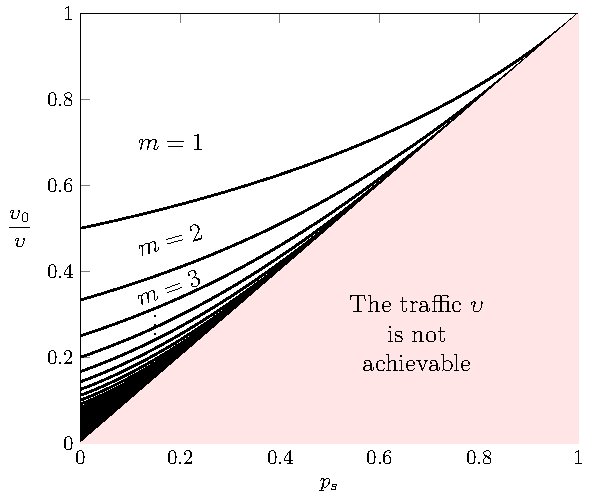
\includegraphics[draft, width=\columnwidth]{Figures/Ch6_opt_m.pdf}
        \fi
        \caption{Optimal choice of $m$ for a given traffic $\upsilon$.}
        \label{fig:opt_m}
    \end{subfigure}%
    \begin{subfigure}{.05\textwidth}
        \hspace{.05\textwidth}
    \end{subfigure}%
    \begin{subfigure}[t]{.45\textwidth}
      \centering
        \if\printfig1
            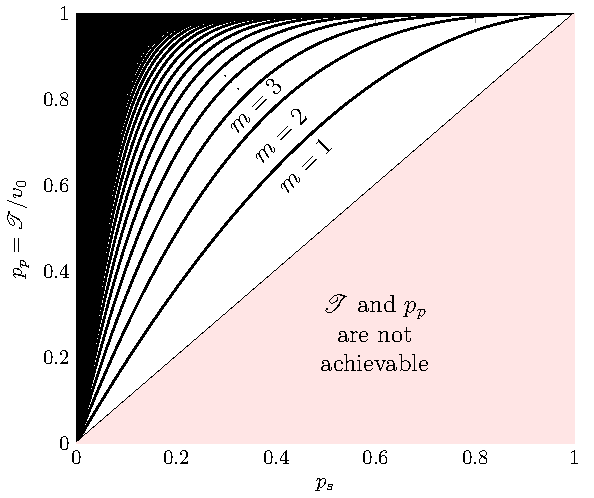
\includegraphics[width=\columnwidth]{Figures/Ch6_opt_m_v2.pdf}
            % 
\begin{tikzpicture}[scale=0.85]

\begin{axis}
[
  title={},
%   width = 212.4pt,
%   width=12cm, height=9cm,
  legend style={at={(0.95,0.95)}, anchor=north east},
  xlabel={$p_s$},
  ylabel={$p_p = \mathscr{T}/\upsilon_0$}, ylabel style={rotate=0},
%  yticklabel=\pgfmathprintnumber{\tick}\\ \%,
  xmin = 0,
  xmax = 1,
  ymin = 0,
  ymax = 1,
%   y tick label style={
%         /pgf/number format/.cd,
%         fixed,
%         fixed zerofill,
%         precision=3,
%         /tikz/.cd
%   },
%   grid = both,
  scale only axis,
]
	\legend{}
    
    \foreach \m in {1,...,20}
        \addplot[thick, domain=0:1, samples=100]{(1-(1-x)^(\m+1))};

    % \foreach \m in {7,9,...,29}
    %     \addplot[thick, domain=0.001:1]{(1-(1-x)^(\m+1))};

    % \foreach \m in {30,40,...,100}
    %     \addplot[thick, domain=0:1]{(1-(1-x)^(\m+1))};
        
    \addplot[thick, domain=0:1]{x};
    
    \addplot[name path=A, thick, domain=0:1, samples=100]{(1-(1-x)^(21+1))};
    \addplot[name path=B, thick, domain=0:1, samples=100]{1};
    \addplot[black] fill between[of=A and B];
    
%     \addplot[blue, dashed] table
%     [
% 		x expr = \thisrow{lam_a}/0.2,
%     	y expr = \thisrow{p_r}
%     ] {./Data/p_th_old.dat};
%     \addplot[green!70!black, dashed] table
%     [
% 		x expr = \thisrow{lam_a}/0.2,
%     	y expr = \thisrow{p_a}
%     ] {./Data/p_th_old.dat};
    
    \fill[color=red!10] (axis cs: 0,0) -- (axis cs: 1,1) -- (axis cs: 1,0);
    
    \draw (axis cs: 0.40,0.58) node[anchor= west, rotate =45] {\large $m=1$};
    \draw (axis cs: 0.35,0.65) node[anchor= west, rotate=45] {\large $m=2$};
    \draw (axis cs: 0.30,0.72) node[anchor= west, rotate=45] {\large $m=3$};
    \draw (axis cs: 0.34,0.81) node[anchor= west, rotate=135] {$\cdots$};
    
    \draw (axis cs: 0.45,0.25) node[anchor= west]
        {\large
        \begin{tabular}{c}
            $\mathscr{T}$ and $p_p$ \\
            are not\\
            achievable
        \end{tabular}
        };
    
    % \node[text width=15mm,anchor=north east] at (1.04,1.07)
    %     {\tiny
    %     \begin{align*}
    %         a   &=0.40\\
    %             &=0.30\\
    %             &=0.20\\
    %             &=0.10\\
    %             &=0.05
    %     \end{align*}
    %     };
\end{axis}

\end{tikzpicture}

        \else
            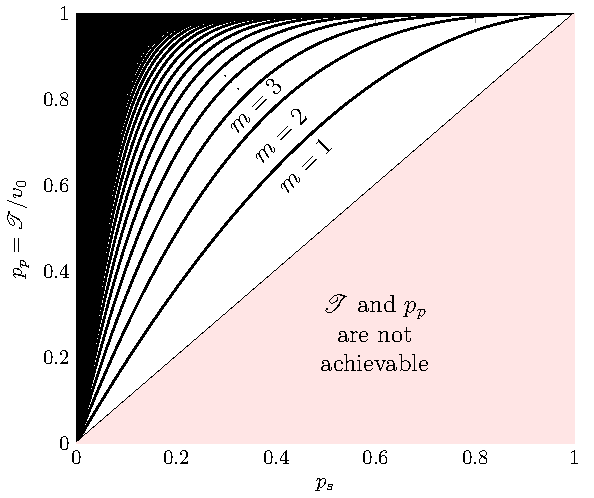
\includegraphics[draft,width=\columnwidth]{Figures/Ch6_opt_m_v2.pdf}
        \fi
        \caption{Optimal choice of $m$ for a given throughput $\mathscr{T}$ or packet success probability $p_p$.}
        \label{fig:opt_m_v2}
    \end{subfigure}
    \caption{}
\end{figure}

Fig.~\ref{fig:opt_m} shows the regions of the $\upsilon_0/\upsilon \times p_s$ plane for which we can choose the best value of the maximum number of retransmissions $m$ when the requirement is a given traffic $\upsilon$.
%
Fig.~\ref{fig:opt_m_v2} is similar to Fig.~\ref{fig:opt_m}, but now for the $\mathscr{T}/\upsilon_0 \times p_s$ plane.

If $p_s^* \upsilon^* < \upsilon_0 \le \upsilon^*$ we can choose as requirement the maximum throughput $\mathscr{T}^*$ or, equivalently, the optimum traffic $\upsilon^*$ and, then, use the figures to find the best value for $m$.
%
The following section provides a numerical example.

%-%-%-%-%-%-%-%-%-%-%-%-%-%-%-%-
\subsection{Numerical Example}

Let us study a simple scenario where the packet success probability function is $p_s(\upsilon) = \euler^{-\alpha\upsilon}$, for some parameter $\alpha>0$. Then, it is easy to show that the maximum throughput is achieved at $\upsilon^* = 1/\alpha$. Then, $p_s^* = 1/\euler$ and $\mathscr{T}^* = (\alpha\euler)^{-1}$.
%
Let us consider that the traffic without retransmission is given by $\upsilon_0 = a \lambda$, where $\lambda > 0$ is a quantity related to the number of users (e.g., the mean number of users per unit of area).

Then, we can plot the mean PAoI (Fig.~\ref{fig:PAoI_a}) as a function of the rate of packets per user $a$, which is a fixed and known quantity in the original problem. This is done for each number of allowed retransmissions $m\in\Z_+$ that satisfies Lemma~\ref{lem:max_lam} with $\upsilon=\upsilon^*$, so that we can adjust the retransmission rate $r^*$ and achieve the maximum throughput $\mathscr{T}^*$.

\begin{figure}[htb]
    \centering
    % \input{Plots/D_a.tex}%
    % \includegraphics[]{Figures/D_a.eps}%
    % \caption{mean delay $\overline D$ as a function of $a$ and for maximum throughput.\vspace{5mm}}
    % \label{fig:D_a}
    %
    \if\printfig1
        % 
\begin{tikzpicture}[scale=0.85]

\begin{axis}
[
  title={},
%   width=12cm, height=9cm,
  width = 0.65\columnwidth,
  legend style={at={(0.95,0.95)}, anchor=north east},
  xlabel={$a$},
  ylabel={mean PAoI [units of time]}, ylabel style={rotate=0},
%  yticklabel=\pgfmathprintnumber{\tick}\\ \%,
  xmin = 0,
  xmax = 1,
  ymin = 0,
  ymax = 8,
%   y tick label style={
%         /pgf/number format/.cd,
%         fixed,
%         fixed zerofill,
%         precision=3,
%         /tikz/.cd
%   },
  grid = both,
  scale only axis,
]
	\legend{}
    
    \addplot[name path=A, dashed] table
	[
		x expr = \thisrow{a},
    	y expr = \thisrow{PAoIinf}
    ] {./Data/PAoI_a_2_part1.dat};
    
    \addplot[name path=B, thick] table
	[
		x expr = \thisrow{a},
    	y expr = \thisrow{PAoIsup}
    ] {./Data/PAoI_a_2_part1.dat};
    
    \addplot[green!10] fill between[of=A and B];
    
    
    \addplot[name path=A, thick] table
	[
		x expr = \thisrow{a},
    	y expr = \thisrow{PAoIinf}
    ] {./Data/PAoI_a_2_part2.dat};

    \addplot[name path=B, thick] table
	[
		x expr = \thisrow{a},
    	y expr = \thisrow{PAoIsup}
    ] {./Data/PAoI_a_2_part2.dat};
    
    \addplot[green!10] fill between[of=A and B];

%%%%%%%%%%%%%%%%%%%%%%%%%%%%%%%%%%%%%%%%%%%%%%%%%%%%%%%%%%

    \addplot[name path=A, dashed] table
	[
		x expr = \thisrow{a},
    	y expr = \thisrow{PAoIinf}
    ] {./Data/PAoI_a_1_part1.dat};
    
    \addplot[name path=B, thick] table
	[
		x expr = \thisrow{a},
    	y expr = \thisrow{PAoIsup}
    ] {./Data/PAoI_a_1_part1.dat};
    
    \addplot[blue!10] fill between[of=A and B];
    
    \addplot[name path=A, thick] table
	[
		x expr = \thisrow{a},
    	y expr = \thisrow{PAoIinf}
    ] {./Data/PAoI_a_1_part2.dat};

    \addplot[name path=B, thick] table
	[
		x expr = \thisrow{a},
    	y expr = \thisrow{PAoIsup}
    ] {./Data/PAoI_a_1_part2.dat};
    
    \addplot[blue!10] fill between[of=A and B];

    
    \foreach \m in {2,...,10}
        \addplot[] table
    	[
    		x expr = \thisrow{a},
        	y expr = \thisrow{m\m}
        ] {./Data/PAoI_1_m234.dat};
    \foreach \m in {2,...,10}
        \addplot[] table
    	[
    		x expr = \thisrow{a},
        	y expr = \thisrow{m\m}
        ] {./Data/PAoI_2_m234.dat};


    \draw[-\arrowhead] (axis cs: 0.70, 1.80) -- (axis cs: 0.55, 3.80);
    \draw (axis cs: 0.55, 3.70) node[anchor= west] {\footnotesize ~$m = 1,2,\dots,\infty$};
    
    \draw[-\arrowhead] (axis cs: 0.40, 4.30) -- (axis cs: 0.25, 7.00);
    \draw (axis cs: 0.25, 7.00) node[anchor= west] {\footnotesize ~$m = 1,2,\dots,\infty$};

    % \draw (axis cs: 0.45,2.00) node[rotate=-20] {\footnotesize$\alpha\lambda_s=1$};
    % \draw (axis cs: 0.20,4.30) node[rotate=-40] {\footnotesize$\alpha\lambda_s=2$};
    \draw (axis cs: 0.43,1.95) node[rotate=-20] {\footnotesize$\alpha\lambda=1$};
    \draw (axis cs: 0.22,4.10) node[rotate=-30] {\footnotesize$\alpha\lambda=2$};

\end{axis}

\end{tikzpicture}
%
        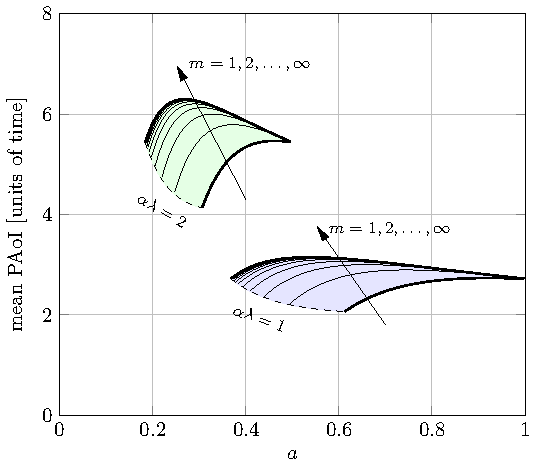
\includegraphics[]{Figures/Ch6_PAoI_a.pdf}
    \else
        
\includegraphics[draft, width=\textwidth]{Figures/placeholder.png}
    \fi
    % \includegraphics[width=0.73\columnwidth]{Figures/PAoI_a_v2.eps}%
    \caption{Mean PAoI $\E[A]$ as a function of $a$ for the maximum $\mathscr{T}$.}
    \label{fig:PAoI_a}
\end{figure}

The blue and green areas correspond to the optimum operating point (adjusting $r\in\R_+$) for each $m\in\N^*\cup\{\infty\}$ and $a\in[1/(\alpha\lambda\euler),1/(\alpha\lambda)]$. The green area is from a system that has twice as many users as the blue area system.
%
As expected, Proposition~\ref{prop:best_m} is observed in Fig.~\ref{fig:PAoI_a}, i.e., the smaller the number of allowed retransmissions $m$, the smaller the mean PAoI.
%
Further, we can see that as we increase $m$, the PAoI performance deteriorates. On the other hand, the region for which we can achieve the maximum throughput increases. For example, to achieve the maximum throughput when $a=1/2$ and $\alpha\lambda=1$, we need $m>1$. More precisely, $m=2$ from Fig.~\ref{fig:opt_m}, since $\upsilon_0/\upsilon^* = 1/2$ and $p_s = 1/\euler\approx 0.368$.
% This is in accordance with Lemma~\ref{lem:max_lam}, and Proposition~\ref{prop:best_m}.

% In Fig.~\ref{fig:D_a}, the mean delay of successful packets is close to $0$ whenever $\upsilon^*$ is close to $\upsilon_0$ ($= a \lambda$) or $p_s^* \upsilon_0$, for which $r^*$ tends to $0$ and $\infty$, respectively. In both cases, the delay tends to $0$, but this is a consequence of our assumption that the transmission time is negligible and in these edge cases it would no longer be valid.
%, because the percentage of dropped packets tends to $1$.
% This is one of the reasons we also used the mean PAoI metric, which elegantly takes into account the data transmission delay caused by dropped packets, so it can no longer be zero.

\begin{remark}
    In our problem, the arrival rate $a$ and initial traffic $\upsilon_0$ are fixed. If such quantities were free, the best approach would be to adjust them and use $m=1$ with a sufficiently small $r$.
\end{remark}

% % % % % % % % % % % % % % 
\section{Summary} \label{sec:summ_P2_02}

In this chapter, we studied a single class random access wireless network with homogeneous traffic, general transmission success probability function, and a retransmission scheme where packets are dropped when new packets arrive at the node or the number of allowed retransmissions is reached.

For a given throughput (or traffic or packet success probability) requirement, we showed that the best approach is to use the minimum number of allowed retransmissions such that, along with an appropriate retransmission rate, the desired requirement is achievable.
%
This approach is optimal for two different metrics: mean delay and mean \textit{Peak-Age-of-Information} (PAoI).
%
This suggests that choosing the smallest number of allowed retransmissions that achieves the network requirements could be an interesting design heuristic.

\chapter{Including Spatial Positions}
\label{cap:P2_03} \thispagestyle{empty}
\def\printfig{1} % Cap. 7
\chapterquote{%
Time and Space\dots It is not nature which imposes them upon us, it is we who impose them upon nature because we find them convenient.}%
{-- Henri Poincar\'e, \textit{The Value of Science} (1905)}

In this chapter\footnote{The present chapter was based on the articles \cite{dester2018} and \cite{dester2021part}.}, we include the spatial position of the nodes in the analysis.
%
Therefore, the transmission success probability $p_s$ can no longer be an arbitrary function of the traffic, because it needs to include the spatial positions into its model.
%
Thus, we need a more specific model for $p_s$, preferably one that entails analytical tractability.
%
In the following section, we propose a model inspired in Proposition~\ref{prop:PPP_ps} and other models adopted throughout the literature.

Another important concept we deal with in this chapter is the \textit{stability} of the queued packets. When a queue is not stable the number of queued packets tends to infinity \textit{almost surely} as time tends to infinity.
%
We are very interested in stable queues, because one of the important metrics, namely the delay, tends to infinity in unstable systems, and that is not desirable.

The additional notations used in this chapter are summarized in Table~\ref{tab:symbols}.
%
\begin{table}[hbt]
    \centering
    \caption{Notations and symbols used in this chapter}
    \label{tab:symbols}
    \setlength{\tabcolsep}{3pt}
    \begin{tabular}{l l}
      \hline
      \hline
      \textbf{Symbol} & \textbf{Definition/explanation} \\
      \hline
        $\alpha\in(2,\infty)$	& path loss exponent \\
        $\delta\in(0,1)$		& $\triangleq 2/\alpha$ \\
        $N \in \N^*$            & number of user classes \\
        $\cal{C}$				& $\triangleq \{1,2,\dots,N\}$, set of classes \\
        $n\in\cal{C}$			& refers to the $n$th user class \\
        $p_n\in(0,1)$			& medium access probability \\
      	$a_n\in(0,1)$			& packet arrival rate per time slot \\
        $\bm{a}\in(0,1)^N$		& $=(a_1,a_2,\dots,a_N)$ \\
        $p_{s,n}\in(0,1)$		& transmission success probability \\
        $\theta_n \in\R_+$		& SIR threshold for successful communication \\
        $\overline{R}_n\in\R_+$	& average transmission distance \\
        $D_n\in(1,\infty)$		& average packet transmission delay \\
        $\bm{D}\in(1,\infty)^N$ & $=(D_1,D_2,\dots,D_N)$ \\
        $P_n\in\R_+$			& transmission power \\
        $\bm{P}\in\R_+^N$ 		& $=(P_1,P_2,\dots,P_N)$ \\
        $\Phi_\TX^{(n)}$	    & Poisson point process for the transmitters \\
        $\lambda_n\in\R_+$		& density of $\Phi_\TX^{(n)}$ \\
        $\psi_n\in\R_+$			& $\triangleq 4\,\overline{R}_n^2 \,\theta_n^{\delta}     \,\pi\delta/\sin(\pi \delta)$ \\
        \hline
      \hline
    \end{tabular}
\end{table}

\newpage

% % % % % % % % % % % % % % % % % % % % % % % % % % 
% % % % % % % % % % % % % % % % % % % % % % % % % % 
\section{Multi-class High-mobility Bipolar Networks} \label{sec:N-class}

\subsection{Main Contributions}
The main contributions of the work presented in this section when compared to the literature, particularly the paper by Stamatiou and Haenggi \cite{stamatiou2010random}, are twofold.
%
Firstly, we have extended the analysis of stability (Definition~\ref{def:stability}) and delay in random-access wireless networks to the case of a network with an arbitrary number $N$ of user classes. As far as we know, this is the first time in the literature the stability region is found in closed form for a network with $N > 3$ different user classes sharing the same channel.
%
Secondly, we have expanded the analysis to show that the channel sharing mechanism in the investigated scenario can be seen as a process of partitioning a fixed and well-defined quantity into portions, each portion allotted to each user class, the size of which varying in accordance with the user class parameters.

More specifically, the novelty of the results on this section are summarized below:
\begin{itemize}[itemsep=3pt,parsep=3pt,topsep=3pt,partopsep=3pt]
    \item We propose a tractable scenario to study the performance and stability of a Poisson network with an arbitrary number $N$ of classes of users sharing the same channel;
    \item a simple and elegant expression relating mean delays, arrival rates, user densities, mean link distances, and bit rates of all $N$ classes is derived for the case of a stable network. This expression clearly shows that each class of user takes a well-defined portion of the available finite resource in the RF channel (Proposition~\ref{prop:identity_1});
    \item a closed form solution (Definition~\ref{def:closed_form}) to the fixed-point system of equations that determine the stationary transmission success probabilities for $N$ user classes is found;
    \item an intuitive equation is presented relating link quality, packet arrival rate, density of users, and stationary mean delay (Proposition 1);
    \item we prove the necessary and sufficient conditions that determine whether a given network is stable (Theorems \ref{TH:NEC_SUFF} and \ref{TH:STABILITY});
    \item we establish a simple necessary condition for stability that does not depend on the transmit powers (Corollary~\ref{cor:stab});
    \item the optimum transmit powers per user class that achieve the optimum stationary mean delays for each user class (Proposition~\ref{prop:opt}) are derived;
    \item the optimum packet arrival rates per user class that achieve the maximum channel throughput per unit of area (Proposition~\ref{prop:eps}) are derived;
    \item we conclude that depending on the channel and user classes, the best strategy to maximize channel throughput is to share the channel, instead of using one single class per channel.
\end{itemize}

% This section is organized as follows: Section \ref{sec:SysMod} describes the model used throughout the chapter and provides some important results from the literature to be used in the following sections;
% Section \ref{sec:N-users} presents the main results of the paper, i.e., necessary and sufficient conditions for stability when we have $N$ interacting user classes, and shows a simple expression for the stationary mean delay and the packet success probability; Section \ref{sec:application} applies the obtained results in two general scenarios: one scenario optimizes the transmission power of different user classes with different delay requirements sharing the same channel and the other optimizes the throughput per unit of area; Section \ref{sec:conclusion} concludes the paper.


\subsection{System Model}

We consider a stationary high-mobility Poisson network with density $\lambda$ on $\R^2$ and with $N$ classes of users that share the same radio frequency channel as defined in the general network model of Chapter~\ref{cap:P2_00}.
%
Time is slotted, $\T=\N$, and for each time slot $t \in \T$ and each user class $n \in \cal{C} \triangleq \{1,2,\dots,N\}$, we have a homogeneous Poisson point process (PPP) denoted by $\Phi_\TX^{(n)}(t)\stackrel{*}{=} \{ X_{i\,n}(t) \}_{i\in\N}$ of density $\lambda_n$ on $\R^2$, which represents the position of the sources. These PPPs are independent from each other and from the past.
%
Furthermore,
\begin{align*}
    \lambda = \sum_{n\in\cal{C}} \lambda_n,
    \quad\text{then,}\quad
    \Phi_\TX(t) = \sum_{n\in\cal{C}} \Phi_\TX^{(n)}(t) \quad\text{for every $t\in\T$}.
\end{align*}

\begin{remark}
    Using the general network model of Chapter~\ref{cap:P2_00}, the set of transmitters $\cal{N}_\TX = \N\times\cal{C}$. Thus, each transmitter should be indexed by a number and a class. However, for ease of notation and since the network is stationary across the users within a class, we shall omit the number and only refer to the class for parameters and metrics.
    %
    For example, the transmission success probability $p_{s,n}$ refers to $p_{s,\N\times\{n\}}$, i.e., it refers to the set of all users from $n$th class (or a typical user of that class).
\end{remark}

\begin{figure}[H]
    \centering
    \if\printfig1
        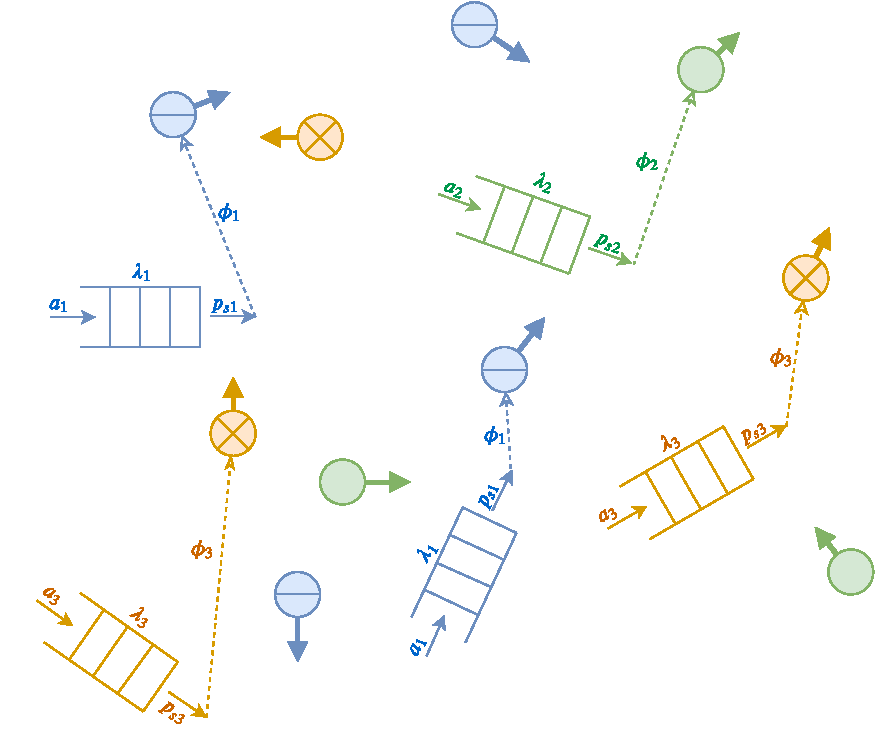
\includegraphics[width=0.8\textwidth]{Figures/Ch7_BipolarQueuedNetwork.pdf}
    \else
        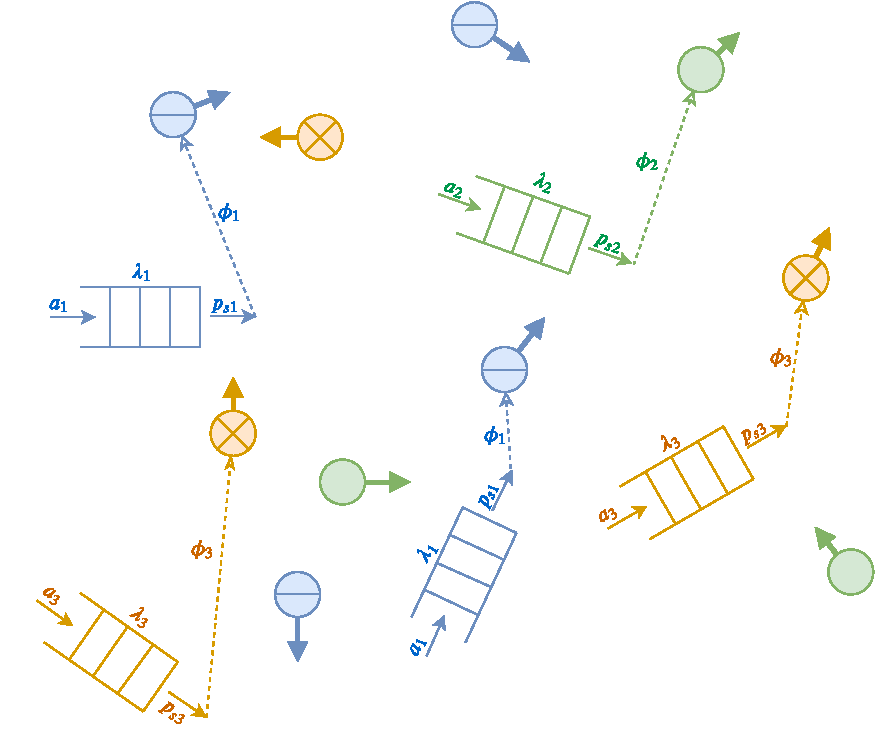
\includegraphics[draft,width=0.8\textwidth]{Figures/Ch7_BipolarQueuedNetwork.pdf}
    \fi
    \caption{Example of a bipolar high-mobility random network with $N=3$ user classes (one for each color). The queues represent the transmitters, and the potential receivers are represented by circular shapes of the corresponding color. The purpose of the arrows is to remember that the nodes are moving. Each transmitter communicates with the closest potential receiver, as it is shown by the dashed lines. Unconnected circles represent inactive receivers. The quantities $\lambda$, $a$, $p_s$ and $\phi$ are related to density of users, rate of arrival of packets, rate of service of packets and link quality, respectively.}
    \label{fig:BipolarNetwork}
\end{figure}

Each transmitter of user class $n$ transmits with power $P_n$ constant over time, and the transmitted signal is subjected to Rayleigh short-term fading and power law path loss function $\ell(r) = r^{-\alpha}, r>0$, where $\alpha>2$ is the path loss exponent.

% For each time slot the position $X_{i\,n}(t)$ of the $i$th transmitter is reallocated following the high-mobility random walk model \cite{baccelli2010stochastic}.
%
% The $i$th transmitter of user class $n$ communicates with a receiver located at $Y_{i\,n}(t)$. Thus, the distance between the $i$th transmitter of class $n$ and its destination is given by $R_{i\,n}(t) = || X_{i\,n}(t) - Y_{i\,n}(t) ||$.
%
We further assume that each transmitter is associated with a ``son'' PPP that models the locations of its potential receivers. The receiver associated with the $i$th transmitter of class $n$ is chosen as the closest point in the respective son PPP as illustrated in Figure~\ref{fig:BipolarNetwork}.

As a consequence, the link distances $\{ R_{i\,n}(t) \}_t$ are iid Rayleigh random variables\footnote{The iid random variables for the link separation distance are of grave importance for the theoretical model. Otherwise, there would exist unstable queues and, consequently, the queueing network would be unstable.} \cite[Eq.~(2.35)]{kingman1992poisson}.
%
Rayleigh distributed link separation distance has been used in several other works investigating similar scenarios (see \cite{haenggi2013diversity}).
%
We denote the mean transmission distance $\E[R_{i\,n}(t)]$ simply by $\overline{R}_n$ because we have stationarity across time and across users of a given class. Then, the density of $R_{i\,n}$ can be expressed as
\begin{align*}
    f_{R_n}(r) = \frac{\pi\,r}{2 \overline{R}_n^2} \exp\!\left[ - \frac{\pi\,r^2}{4\overline{R}_n^2}\right], \qquad r\in\R_+.
\end{align*}

The occupation of the buffer at each transmitter is represented by its queue length $\{ Q_{i\,n}(t) \}_t$ of infinite capacity.
%
The packet arrival probability at each queue is denoted by $a_n$ and the medium access probability by $p_n$.
%
Within each slot, the first event to take place for each transmitter with a non-empty queue is the medium access decision with probability $p_n$. If it is granted access and the signal to interference ratio (SIR) %\footnote{We assume thermal noise is negligible; refer to \cite{haenggi2012stochastic} for further details.}
is greater than a threshold $\theta_n>0$, a packet is successfully transmitted and leaves the queue. Then, we have the arrival of the next packet with probability $a_n$. The last event to take place is the displacement of the transmitters and destinations.

The queue lengths of the $i$th transmitter, user class $n$ are Markov chains represented by
\begin{equation*}
	Q_{i\,n}(t+1) = (Q_{i\,n}(t) - B_{i\,n}(t))_+ + E_{i\,n}(t), \quad t \in \N,
\end{equation*}
where $(\cdot)_+ \triangleq \max\{\cdot,0\}$, $\{E_{i\,n}(t)\}_t$ are iid Bernoulli random variables of parameter $a_n$, i.e., $E_{i\,n}(t)\sim\mathscr{B}(a_n)$ and represents the arrival process,
$
	B_{i\,n}(t) = e_{i\,n}(t)\,\ind\{\text{SIR}_{i\,n}(t)>\theta_{n}\}
$
represents the departure process, where $\{e_{i\,n}(t)\}_t$ are iid Bernoulli random variables of parameter $p_n$, i.e., $e_{i\,n}(t)\sim\mathscr{B}(p_n)$, and the constant $\theta_n > 0$ represents the SIR threshold for successful communication.

\begin{remark}
        In view of the model of Chapter~\ref{cap:P2_00}, we have that the arrival point process $A_{i\,(n)}$ is a Bernoulli point process of parameter $a_n$, the access point process $T_{i\,(n)}$ is a Bernoulli point process of parameter $p_n$ and the transmissions times $T_{i\,(n)}^*$ is a thinning of $T_{i\,(n)}$ conditioned to the corresponding queue being non-empty, and the success probability model $\mathscr{S}(f) = \ind\{f(0) > 1\}$, where $f(t') = \SIR_{i\,n}(t-t')/\theta_n$.
\end{remark}

% % % % % % % % % % % % % % % % % % % % % % % % % % % % % %
\subsection{Analysis and Results}
\label{ssec:N-users}

From the stationarity across users of a class and ergodicity regarding time (if the system is stable), the transmission success probability $p_{s,n}$ is the limiting probability of a successful transmission from a typical user of class $n$, i.e., $$p_{s,n} = \lim_{t\to\infty} \P(\mathrm{SIR}_{i,n}(t) > \theta_n).$$

\begin{note}
    Remember that, \textit{à priori}, we do not need to take $t\to\infty$, any $t$ would suffice in an ergodic process.
    %
    However, as discussed in Section~\ref{sec:poisson_network} we would have to start the system at $-\infty$ or start the system distributed according to the stationary distribution.
\end{note}

The stationary mean delay $D_n$ to transmit packets of class $n$ is defined as the limiting ($t\to\infty$) expected time a packet spends in the buffer and the server.
%
See Theorem~\ref{th:little}.
% For each time slot and for each class we have an independent homogeneous PPP, which is stationary and isotropic (invariant to translation and rotation, respectively).

% The following results from the literature are used in many proofs throughout the chapter. In a wireless network, let us assume that \textit{(i)} the separation distance between a given pair TX - RX is equal to $r$, \textit{(ii)} the positions of the interferers (users who will transmit packets in a given time slot) follow a PPP of density $\lambda_\mathrm{eff}$, and \textit{(iii)} every transmitter has the same transmit power. Then, the probability of a successful transmission between TX and RX is given by \cite[Sec.~III.A]{haenggi2009stochastic}
% \begin{align}
% 	\P(\mathrm{SIR} > \theta) &= \E[\euler^{-\theta r^\alpha I}] \nonumber\\
%     	&= \exp\left( - \pi\,\Gamma(1+\delta) \Gamma(1-\delta)\,\theta^{\delta}\,r^2\,\lambda_\mathrm{eff} \right),
% \end{align}
% where $\delta \triangleq 2/\alpha$ and $I \triangleq \sum_{X\in\Phi} ||X||^{-\alpha}$ is the interference received by RX normalized by the transmit power and $\Phi$ is a PPP of density $\lambda_\mathrm{eff}$, which is the effective density of active sources.
%

% As described in the previous section, we consider a network with $N$ classes of users.
%
The following proposition presents the stationary success probability and mean delay when transmitting a packet in a stable network. The results that guarantee stability are presented later in the sequence, in Theorem~\ref{TH:NEC_SUFF}.

\begin{proposition} \label{prop:psk}
	If the network is stable, then the stationary success probability and mean delay for a typical user of class $n \in \cal{C}$ are given by
	\begin{align}
    	p_{s,n} &= \left( 1 + \dfrac{\psi_n}{P_n^\delta}\, 
        \dfrac{\sum_j P_j^\delta\,a_j\lambda_j}
        {1 - \sum_j \psi_j\,a_j\lambda_j} \right)^{-1},\label{eq:psn}\\ 
        D_n &= \dfrac{1 - a_n}{p_n\,p_{s,n} - a_n},	\label{eq:Dn}
    \end{align}
    where the sums are taken over the set of user classes $\cal{C}$, ${\delta \triangleq 2/\alpha}$, and 
    \begin{equation}\label{eq:DefPhi}
        \psi_n
            \triangleq 4\,\Gamma(1+\delta) \Gamma(1-\delta) \overline{R}_n^2 \theta_n^\delta
            = 4\,\overline{R}_n^2\,\theta_n^{\delta}\, \frac{\pi\delta}{\sin(\pi \delta)}.
    \end{equation}
\end{proposition}

\begin{proof}
    First, we need to calculate the transmission success probability for a given traffic and a given link distance.
    %
    Using the reasoning of Proposition~\ref{prop:PPP_ps} for the case of several classes of users, we have
    \begin{align} \label{eq:P_SIR}
    	\P(\text{SIR}_{i\,n}(t)>\theta_n \mid R_{i\,n}) &= \E\!\left[\exp\left(-\frac{\theta\,R_{i\,n}^\alpha}{P_n} \sum_{k\in\cal{C}} P_k\,I_k\right)\right]\nonumber\\
        	&= \prod_{k\in\cal{C}} \E\!\left[\exp\left(-\theta\,R_{i\,n}^\alpha\frac{P_k}{P_n} I_k\right)\right] \nonumber\\
            &= \prod_{k\in\cal{C}} \exp\!\left( - \pi R_{i\,n}^2\, \theta^{\delta}\,\frac{\pi\delta}{\sin(\pi\delta)} \frac{P_k^\delta}{P_n^\delta}\lambda_\mathrm{eff}^{(k)}(t)\right) \nonumber\\
        	&= \exp\!\left( - \pi R_{i\,n}^2\,\theta^{\delta}\,\frac{\pi\delta}{\sin(\pi\delta)} \,\sum_{k\in\cal{C}}\frac{P_k^\delta}{P_n^\delta}\lambda_\mathrm{eff}^{(k)}(t)\right),
    \end{align}
    where $I_n$ is the interference from the $n$th class normalized by the transmit power, and $\lambda_{\mathrm{eff}}^{(n)}$ is the density of the thinned Poisson point process $\Phi_\TX^{(n)}$ by the nodes that are transmitting.
    %
    It is assumed that $\{I_n\}_{n \in \cal{C}}$ is iid.

    As $t\to\infty$, the effective PPP density of active sources $\lambda_\mathrm{eff}^{(n)}$ for each user class $n\in\cal{C}$ converges (by hypothesis) to $\lambda_n\,p_n\,\rho_n$, where $\rho_n = a_n/(p_n\,p_{s,n})$ is the load of the queue (or the probability of having a non-empty queue), which is the ratio between the arrival rate and the service rate of packets. Thus, $\lambda_\mathrm{eff}^{(n)} = \lambda_n\,a_n/p_{s,n}$.

    Then, to calculate the transmission success probability $p_{s,n}$, we use \eqref{eq:P_SIR}. Thus, by deconditioning the transmission success probability on $R_{i\,n}$, we take into account that $R_{i\,n}$ is Rayleigh distributed, that is
    \begin{align} \label{eq:aux_psk}
    	p_{s,n} &= \lim_{t\to\infty}\P(\text{SIR}_{i\,n}(t)>\theta_n) \nonumber\\
        	&= \int_0^\infty \lim_{t\to\infty} \P(\text{SIR}_{i\,n}(t)>\theta_n
            	\mid R_{i\,n}(t) = r)\,f_{R_n}(r)\,\mathrm{d}r \nonumber\\
            &= \int_0^\infty \frac{\pi r}{2 \overline{R}_n^2} \exp\!\left[ - \frac{\pi\,r^2}{4\overline{R}_n^2} \left(1+\psi_n\sum_{k\in\cal{C}}\frac{P_k^\delta}{P_n^\delta}\lambda_\mathrm{eff}^{(k)}\right)\right]\mathrm{d}r \nonumber\\
            &= \left( 1 + \dfrac{\psi_n}{P_n^\delta}
      			\sum_{k\in\cal{C}} P_k^\delta \dfrac{a_k\lambda_k}{p_{s,k}} \right)^{-1}.
    \end{align}
    This expression can be rearranged as
    \begin{equation} \label{eq:psk_equivalence}
    	\dfrac{P_n^\delta}{\psi_n} \left( \dfrac{1-p_{s,n}}{p_{s,n}}\right) = 
        \sum_{k\in\cal{C}} P_k^\delta \dfrac{a_k\lambda_k}{p_{s,k}}.
    \end{equation}
    Note that the right-hand side of \eqref{eq:psk_equivalence} does not depend on $n$. Then, for all $j\in\cal{C}$, we have%
    \begin{equation} \label{eq:Pi_Pk}
    	\dfrac{P_j^\delta}{\psi_j} \left( \dfrac{1-p_{s,j}}{p_{s,j}}\right) = 
        \dfrac{P_n^\delta}{\psi_n} \left( \dfrac{1-p_{s,n}}{p_{s,n}}\right).
    \end{equation}
    For each $j$, we can solve the above equation for $p_{s,j}$ and plug it into the sum of \eqref{eq:aux_psk}. Then, we can solve it for $p_{s,n}$, which ends the proof for the $p_{s,n}$.
    
    The buffer (plus server) is a discrete time Geo/Geo/1 queue (Definition~\ref{def:geo/geo/1}) at stationary \cite{stamatiou2010random} and the equation for the delay $D_n$ comes from Theorem~\ref{th:geo/geo/1}.
\end{proof}

The following theorem shows the conditions for which the network is stable, i.e., it presents the region formed by all arrival rates $\bm{a}$ that make the system stable.

\begin{theorem} \label{TH:NEC_SUFF}
	A necessary and sufficient condition for the system network to be stable is that $\bm{a} \in \bigcup_{\nu\in\cal{V}} \cal{E}_\nu$, where $\cal{V}$ is the space of all bijective functions from $\cal{C}$ to $\cal{C}$ and $\cal{E}_\nu$ is defined below with the convention $\sum_{k=1}^0 \cdot = 0$.
	\begin{align} \label{eq:stab_long}
    	\cal{E}_{\nu} \triangleq \Bigg\{ \bm{a} \in [0,1)^N \Bigm\vert~ 
    	& 0 \le 
        \dfrac{\psi_{\nu(n)}}{P_{\nu(n)}^\delta}\dfrac{a_{\nu(n)}}{p_{\nu(n)}-a_{\nu(n)}} \nonumber\\
        & < \dfrac{ 1 - \sum_{k=1}^{n-1} \psi_{\nu(k)} a_{\nu(k)} \lambda_{\nu(k)} }
        {\sum_{k=1}^{n-1} P_{\nu(k)}^{\delta} a_{\nu(k)}\lambda_{\nu(k)} +
        \sum_{k=n}^N P_{\nu(k)}^\delta p_{\nu(k)}\lambda_{\nu(k)}},
        \quad n \in \cal{C} \Bigg\}.
    \end{align}
\end{theorem}
%
\begin{proof}
    Using stochastic dominance through dominant networks \cite[Section~2.1.2]{kompella2014stable}, it is possible to derive necessary and sufficient conditions for stability.
    %
    A dominant network behaves exactly the same as the original network, except that all user classes in a subset $\cal{D}$ of $\cal{C}$ transmit dummy packets.
    %
    Thus, the dominant network have more or the same number of buffered packets as the original network  \textit{almost surely}.
    %
    Then, if the dominant network is stable, the original network is stable as well. On the other hand, if the queues of the user classes in $\cal{D}$ are not empty in the original network, then this system behaves exactly like the dominant network, i.e, both systems are \emph{indistinguishable}, see Definition~\ref{def:indistinguishable} and \cite[Section~3.2]{szpankowski1994stability}.
    %
    Therefore, if the dominant network is unstable, then the original network is unstable as well.
    %
    In order to have necessary and sufficient conditions, we must perform this verification for all $\cal{D} \subset \cal{C}$.
    
    Let us start with $\cal{D}=\cal{C}$, i.e., all users transmit dummy packets. For each step of the verification, we remove the stable user class from the set $\cal{D}$. This procedure repeats until the set $\cal{D}$ becomes empty. In order to attain stability of the dominant network we must have an arrival rate smaller than the service rate (Theorem~\ref{th:loynes}). Thus, a sufficient condition for the first user class stability is, for any queue $i$ of this class (by symmetry),
    \begin{equation*}
    	a_1 < p_1\,\P(\widetilde{\text{SIR}}_{i,1} > \theta_1) = p_1 \left( 1 + \dfrac{\psi_1}{P_1^\delta} \sum_{k=1}^N P_k^\delta\,p_k\lambda_k \right)^{-1},
    \end{equation*}
    where $\widetilde{\text{SIR}}$ represents the signal-interference ratio in the dominant network and the second equality comes from the same procedure to obtain \eqref{eq:aux_psk} with $\lambda_\mathrm{eff}^{(n)} = \lambda_n$ (all users are active, since every TX transmits dummy packets).
    %
    This guarantees stability for the first user class. Let us remove it from the set $\cal{D}$. Then, we calculate the stationary success probability of the first user class $\widetilde{p}^{(1)}_{s,1}$ for this dominant network. At steady state, we have
    \begin{equation*}
    	\widetilde{p}^{(1)}_{s,1} = \left( 1 + \dfrac{\psi_1}{P_1^\delta} \left( P_1^\delta\,p_1\lambda_1\dfrac{a_1}{p_1\widetilde{p}^{(1)}_{s,1}} + \sum_{k=2}^N P_k^\delta\,p_k\lambda_k \right) \right)^{-1},
    \end{equation*}
    which can be solved for $\widetilde{p}^{(1)}_{s,1}$,
    \begin{equation*}
    	\widetilde{p}^{(1)}_{s,1} = \dfrac{1 - \psi_1\,\lambda_1\,a_1}{1 + \frac{\psi_1}{P_1^\delta} \sum_{k=2}^N P_k^\delta\,p_k\lambda_k}.
    \end{equation*}
    The next step is to verify the conditions of stability for the second user class, when the first user class is at steady state. After that, we remove the second user class from the set $\cal{D}$ and calculate the stationary success probability of the two stable user classes in the dominant network. We repeat these steps until we remove all user classes, \textit{i.e}, $\cal{D} = \{\}$. We show this by induction; we suppose stability of the user classes $1,2,\dots,j-1$. Let $\cal{D} = \{j,j+1,\dots\,N\}$; the $j$th user class is stable, given that all the user classes in $\cal{C}\setminus\cal{D}$ are stable, when
    \begin{align} \label{eq:aux_aj}
    	a_j 
    	&< p_j\,\P(\widetilde{\text{SIR}}_{i,j} > \theta_j) \nonumber\\
    	&= p_j \left( 1+\dfrac{\psi_j}{P_j^\delta} 
            \left( \sum_{k=1}^{j-1} P_k^\delta\,\lambda_k\,\dfrac{a_k}
            {\widetilde{p}^{(j)}_{s,k}} + \sum_{k=j}^N P_k^\delta\,p_k\lambda_k \right) \right)^{-1},
    \end{align}
    where $\widetilde{p}^{(j)}_{s,k}$ is the $k$th user class success probability ($1 \leq k < j$) at steady state in the dominant network at the $j$th step. To calculate this probability, we must solve the following system of equations. For $k \in \{1,2,\dots,j-1\}$
    \begin{equation*}
    	\widetilde{p}^{(j)}_{s,k} = \left( 1 + \dfrac{\psi_k}{P_k^\delta}
        \left( \sum_{\ell = 1}^{j-1} P_\ell^\delta\,\lambda_\ell\,
        \dfrac{a_\ell}{\widetilde{p}^{(j)}_{s,\ell}} + 
        \sum_{\ell = j}^{N} P_\ell^\delta\,p_\ell\lambda_\ell \right) \right)^{-1}.
    \end{equation*}
    Using an analogous approach as the one presented in the proof of Proposition~\ref{prop:psk}, we have that for $k \in \{1,2,\dots,j-1\}$,
    \begin{equation*}
    	\widetilde{p}^{(j)}_{s,k} =
        \left( 1 + \dfrac{\psi_k}{P_k^\delta} 
        \dfrac{ \sum_{\ell=1}^{j-1} P_\ell^\delta\,a_{\ell}\,\lambda_\ell +
        \sum_{\ell=j}^{N} P_\ell^\delta\,p_\ell\lambda_\ell }
        { 1 - \sum_{\ell=1}^{j-1} \psi_{\ell}\,a_{\ell}\,\lambda_\ell} 
        \right)^{-1}.
    \end{equation*}
    Comparing the last two equations, it is easy to see that
    \begin{align*}
    	\sum_{\ell = 1}^{j-1} P_\ell^\delta\,\lambda_\ell\,
        &\dfrac{a_\ell}{\widetilde{p}^{(j)}_{s,\ell}} + 
        \sum_{\ell = j}^{N} P_\ell^\delta\,p_\ell\,\lambda_\ell = \dfrac{ \sum_{\ell=1}^{j-1} P_\ell^\delta\,a_{\ell}\,\lambda_\ell +
        \sum_{\ell=j}^{N} P_\ell^\delta\,p_\ell\lambda_\ell }
        { 1 - \sum_{\ell=1}^{j-1} \psi_{\ell}\,a_{\ell}\,\lambda_\ell } .
    \end{align*}    
    Finally, we can use this result to rewrite \eqref{eq:aux_aj} as, for all $j \in \cal{C}$,
    \begin{equation*}
        0 \le
    	\dfrac{\psi_j}{P_j^\delta}\,\dfrac{a_j}{p_j-a_j} <
        \dfrac{1 - \sum_{k=1}^{j-1} \psi_k\,a_k\,\lambda_k}
        {\sum_{k=1}^{j-1} P_k^\delta\,a_k\lambda_k +
        \sum_{k=j}^N P_k^\delta\,p_k\lambda_k}.
    \end{equation*}
    This concludes the proof since the extension for the other partitions of $\cal{C}$ is analogous.
\end{proof}

Theorem~\ref{TH:NEC_SUFF} requires verifying $N\!\times\!N!$ inequalities, whereas the following theorem is equivalent and it involves only $N$ inequalities.
%
Thus, Theorem~\ref{TH:STABILITY} presents a simpler form of verifying the conditions for stability.
% Also, it relates (in the proof) the stability condition with the stationary mean delays $\bm{D}$.
However, we cannot prove \ref{TH:STABILITY} without \ref{TH:NEC_SUFF}.

\begin{theorem}[\textbf{Network Stability}] \label{TH:STABILITY}
	The system network is stable if and only of $\bm{a}\in\cal{R}$,
    \begin{align*}
    	\cal{R}
        \triangleq \bigg\{ \bm{a}\in[0,1)^N \bigm\vert ~ a_n < p_n, \dfrac{\psi_n}{P_n^\delta}\,\dfrac{a_n}{p_n-a_n} < 
        \dfrac{1 - \sum_{k} \psi_k\,a_k \lambda_k}
        {\sum_{k} P_k^{\delta}\,a_k \lambda_k} 
        \quad\forall n \in \cal{C}  \bigg\}.
        % &= \bigg\{ \bm{a}\in[0,1)^N \bigm\vert ~ a_n < p_n, \\
        % &\hspace{2mm} \dfrac{\psi_n}{P_n^\delta}\,\dfrac{a_n}{p_n-a_n} < 
        % \dfrac{1 - \sum_{k \neq n} \psi_k\,a_k\,\lambda_k}
        % {P_n^\delta\,p_n\lambda_n + \sum_{k \neq n} P_k^{\delta}\,a_k\,\lambda_k}
        % ~\forall n \in \cal{C}  \bigg\}.
    \end{align*}
\end{theorem}

\begin{proof}
	The proof consists of showing that the set $\cal{R}$ is equal to the set defined in Theorem~\ref{TH:NEC_SUFF}.
    %
    First, let us prove that $\bigcup_{\nu\in\cal{V}} \cal{E}_\nu \subset \cal{R}$.
    %
    For that we suppose $\bm{a} \in \cal{E}_\nu$ and we show $\bm{a} \in \cal{R}$ for all $\nu\in\cal{V}$ by induction.
    %
    For simplicity of exposition let us take $\cal{E}_\nu$ with $\nu: n \longmapsto n$, $n\in\cal{C}$.
    %
    We assume the inequality
    \begin{align}
        \dfrac{\psi_{N-j}}{P_{N-j}^\delta}\,\dfrac{a_{N-j}}{p_{N-j}-a_{N-j}} 
        & < \dfrac{1 - \sum_{k=1}^{N} \psi_k\,a_k \lambda_k}{\sum_{k=1}^{N} P_k^\delta\,a_k\lambda_k}. \label{eq:th2_basecase}
    \end{align}
    %
    is true for all $j\in\{0,\dots,m-1\}$ and we prove that it is also true for $j=m$.
    %
    First, we have to prove the base case $m = 1$.
    %
    Since $\bm{a}\in \cal{E}_\nu$, then for $j=0$ ($n=N$)
    %
    \begin{align*}
        	\dfrac{\psi_N}{P_N^\delta}\,\dfrac{a_N}{p_N-a_N} 
        	& < \dfrac{1 - \sum_{k=1}^{N-1} \psi_k\,a_k \lambda_k}{\sum_{k=1}^{N-1} P_k^\delta\,a_k\lambda_k + P_N^\delta\,p_N\lambda_N} \\
        & = \dfrac{1 - \sum_{k=1}^{N} \psi_k\,a_k \lambda_k + \psi_N\,a_N \lambda_N}{\sum_{k=1}^{N} P_k^\delta\,a_k\lambda_k + P_N^\delta\,(p_N-a_N)\lambda_N}.
    \end{align*}
    %
    Then, using simple manipulations, we can show that the above inequality is equivalent to
    %
    \begin{align*}
        	\dfrac{\psi_N}{P_N^\delta}\,\dfrac{a_N}{p_N-a_N} 
        	& < \dfrac{1 - \sum_{k=1}^{N} \psi_k\,a_k \lambda_k}{\sum_{k=1}^{N} P_k^\delta\,a_k\lambda_k}.
    \end{align*}
    %
    Thus, the base case $m = 1$ is true.
    %
    Now, for $j=m$ and $\bm{a}\in \cal{E}_\nu$, we know that
    \begin{align*}
        \dfrac{\psi_{N-m}}{P_{N-m}^\delta}\,\dfrac{a_{N-m}}{p_{N-m}-a_{N-m}}
        & < \dfrac{1 - \sum_{k=1}^{N-m-1} \psi_k\,a_k \lambda_k}
        	{\sum_{k=1}^{N-m-1} P_k^\delta\,a_k\lambda_k 
        	    + \sum_{k=N-m}^{N} P_k^\delta\,p_k\lambda_k} \\
        & = \dfrac{1 - \sum_{k=1}^{N} \psi_k\,a_k \lambda_k 
                + \sum_{k=N-m}^{N} \psi_k\,a_k \lambda_k}
            {\sum_{k=1}^{N} P_k^\delta\,a_k\lambda_k 
                + \sum_{k=N-m}^{N} P_k^\delta\,(p_k-a_k)\lambda_k}.
    \end{align*}
    Through simple manipulations we can show that the above inequality is equivalent to
    \begin{align*}
        & \dfrac{\psi_{N-m}}{P_{N-m}^\delta}\,\dfrac{a_{N-m}}{p_{N-m}-a_{N-m}} < \dfrac{1 - \sum_{k=1}^{N} \psi_k\,a_k \lambda_k 
                + \sum_{k=N-m+1}^{N} \psi_k\,a_k \lambda_k}
            {\sum_{k=1}^{N} P_k^\delta\,a_k\lambda_k 
                + \sum_{k=N-m+1}^{N} P_k^\delta\,(p_k-a_k)\lambda_k}.
    \end{align*}
    Now, we only need to verify that
    \begin{align*}
    &\dfrac{1 - \sum_{k=1}^{N} \psi_k\,a_k \lambda_k 
                + \sum_{k=N-m+1}^{N} \psi_k\,a_k \lambda_k}
            {\sum_{k=1}^{N} P_k^\delta\,a_k\lambda_k 
                + \sum_{k=N-m+1}^{N} P_k^\delta\,(p_k-a_k)\lambda_k} < \dfrac{1 - \sum_{k=1}^{N} \psi_k\,a_k \lambda_k}
            {\sum_{k=1}^{N} P_k^\delta\,a_k\lambda_k}.
    \end{align*}
    Again, simple manipulations lead to the equivalent inequality
    \begin{align*}
    &\dfrac{\sum_{k=N-m+1}^{N} \psi_k\,a_k \lambda_k}
            {\sum_{k=N-m+1}^{N} P_k^\delta\,(p_k-a_k)\lambda_k}
        < \dfrac{1 - \sum_{k=1}^{N} \psi_k\,a_k \lambda_k}
            {\sum_{k=1}^{N} P_k^\delta\,a_k\lambda_k},
    \end{align*}
    which is true from the base case. This can be seen by multiplying  \eqref{eq:th2_basecase} by $P^\delta_{N-j}(p_{N-j}-a_{N-j})$ at both sides of the inequality and summing over $j\in\{0,\dots,m-1\}$. Thus, $\cal{E}_\nu \subset \cal{R}$ for the mapping $\nu: n \longmapsto n$. The extension for another instances of $\nu\in\cal{V}$ is analogous. This concludes the proof that $\bigcup_{\nu\in\cal{V}} \cal{E}_\nu \subset \cal{R}$.
    %
    
    However, we still need to prove the converse, that is ${\cal{R} \subset \bigcup_{\nu\in\cal{V}}} \cal{E}_\nu$.
    %
    Note that the set of arrival rates that makes the system stable in Theorem~\ref{TH:NEC_SUFF} requires that at least one $a_n$ ($n\in\cal{C}$) satisfies
    \begin{equation} \label{eq:aux_stab_first}
    	\dfrac{\psi_n}{P_n^\delta}\,\dfrac{a_n}{p_n-a_n} <
        \dfrac{1}{\sum_{k=1}^N P_k^\delta\,p_k \lambda_k}.
    \end{equation}
    	Let us show that $\cal{R}$ requires the same restriction by contradiction. Suppose that there exist $\bm{a}\in\cal{R}$ such that
        %
    \begin{equation} \label{eq:aux_contr0}
        \dfrac{\psi_n}{P_n^\delta}\,\dfrac{a_n}{p_n-a_n} \ge
        \dfrac{1}{\sum_{k=1}^N P_k^\delta\,p_k \lambda_k}
        \quad \forall n \in \cal{C}.
    \end{equation}
    %
    Multiplying \eqref{eq:aux_contr0} by $P_n^\delta(p_n-a_n)\lambda_n > 0$ at both sides and summing over $n\in\cal{C}$ we have
    %
    \begin{align*}
        \sum_{n=1}^N \psi_n a_n \lambda_n 
            \ge \frac{\sum_{n=1}^N P_n^\delta (p_n-a_n) \lambda_n}
            {\sum_{k=1}^N P_k^\delta\,p_k \lambda_k},
    \end{align*}
    %
    which is equivalent to
    %
    \begin{align} \label{eq:aux_case0}
        \left(\sum_{n=1}^N \psi_n a_n \lambda_n \right)
            \left(\sum_{k=1}^N P_k^\delta\,p_k \lambda_k \right)
            \ge \sum_{n=1}^N P_n^\delta (p_n-a_n) \lambda_n.
    \end{align}
    %
    Since $\bm{a}\in\cal{R}$, then
    \begin{align} \label{eq:aux_theo2}
        \dfrac{\psi_n}{P_n^\delta}\,\dfrac{a_n}{p_n-a_n} < 
            \dfrac{1 - \sum_{k} \psi_k\,a_k \lambda_k}
            {\sum_{k} P_k^{\delta}\,a_k \lambda_k} \quad \forall n\in\cal{C}.
    \end{align}
    %
    Again, multiplying \eqref{eq:aux_theo2} by $P_n^\delta(p_n-a_n)\lambda_n > 0$ at both sides, summing over $n\in\cal{C}$ and performing some manipulations we have
    %
    \begin{align} \label{eq:aux_theo2_case0}
        &\left(\sum_{n=1}^N \psi_n a_n \lambda_n \right)
            \left(\sum_{k=1}^N P_k^\delta\,a_k \lambda_k \right) < \left(1 - \sum_{k=1}^N \psi_k\,a_k \lambda_k \right)\left(\sum_{n=1}^N P_n^\delta (p_n-a_n) \lambda_n\right).
    \end{align}
    %
    Then, through some manipulations on \eqref{eq:aux_case0} and \eqref{eq:aux_theo2_case0}, we have
    %
    \begin{align*}
        0 &\le \sum_{n=1}^N P_n^\delta a_n \lambda_n - \left(1 - \sum_{k=1}^N \psi_k\,a_k \lambda_k \right)\left(\sum_{n=1}^N P_n^\delta p_n \lambda_n\right) < 0,
    \end{align*}
    which clearly is a contradiction, since $\cal{R}$ is a non-empty set. Thus, there exists at least one $a_n$, $n\in\cal{C}$ that satisfies \eqref{eq:aux_stab_first}.
    %
    For simplicity of exposition, let us suppose that the arrival rate $a_n$ that satisfies this restriction is from the first user class ($n=1$). The next step is to show that as in the set $\bigcup_{\nu\in\cal{V}}\cal{E}_\nu$, the set $\cal{R}$ also requires that we have at least one $a_n$, aside from $a_1$, that satisfies
    %
    \begin{equation*}
    	\dfrac{\psi_n}{P_n^\delta}\,\dfrac{a_n}{p_n-a_n} <
        \dfrac{1-\psi_1\,\lambda_1\,a_1}{P_1^\delta\,a_1\lambda_1+
        \sum_{k=2}^N P_k^\delta\,p_k\lambda_k}.
    \end{equation*}
    %
    We can also prove this by contradiction and then, for simplicity of exposition, suppose that $a_2$ is the one that satisfies this restriction. We repeat this procedure until we reach all user classes. Let us show the $j$th step for completeness, $j\in\cal{C}$. Suppose that for all $n \in \{j,j+1,\dots,N\}$,
    %
    \begin{align} \label{eq:aux_contr_j}
        \dfrac{\psi_n}{P_n^\delta}\dfrac{a_n}{p_n-a_n}
        \ge \dfrac{ 1 - \sum_{k=1}^{j-1} \psi_k a_k \lambda_k }
        {\sum_{k=1}^{j-1} P_k^{\delta} a_k\lambda_k +
        \sum_{k=j}^N P_k^\delta p_k\lambda_k}.
    \end{align}
    Multiplying \eqref{eq:aux_contr_j} by $P_n^\delta(p_n-a_n)\lambda_n > 0$ at both sides, summing over $n\in\{j,j+1,\dots,N\}$ and manipulating we have
    %
    \begin{align} \label{eq:aux_case_j}
        &\left(\sum_{n=j}^N \psi_n a_n \lambda_n \right)\!
            \left(\sum_{k=1}^N P_k^\delta\,a_k \lambda_k + \sum_{k=j}^N P_k^\delta\,(p_k-a_k) \lambda_k \right) \ge \left( 1 - \sum_{k=1}^{j-1} \psi_k a_k \lambda_k \right)\!
            \left( \sum_{n=j}^N P_n^\delta (p_n-a_n) \lambda_n \right).
    \end{align}
    %
    Once again, multiplying \eqref{eq:aux_theo2} by $P_n^\delta(p_n-a_n)\lambda_n > 0$ at both sides, summing over $n\in\{j,j+1,\dots,N\}$ and manipulating we have
    %
    \begin{align} \label{eq:aux_theo2_case_j}
        &\left(\sum_{n=j}^N \psi_n a_n \lambda_n \right)
            \left(\sum_{k=1}^N P_k^\delta\,a_k \lambda_k \right) < \left(1 - \sum_{k=1}^N \psi_k\,a_k \lambda_k \right)\left(\sum_{n=j}^N P_n^\delta (p_n-a_n) \lambda_n\right).
    \end{align}
    %
    Then, through some manipulations on \eqref{eq:aux_case_j} and \eqref{eq:aux_theo2_case_j}, we have
    %
    \begin{align*}
        0 &\le \left(1 - \sum_{k=1}^N \psi_k\,a_k \lambda_k \right)\left(\sum_{n=j}^N P_n^\delta (p_n-a_n) \lambda_n\right) - \left(\sum_{n=j}^N \psi_n a_n \lambda_n \right)
            \left(\sum_{k=1}^N P_k^\delta\,a_k \lambda_k \right) < 0.
    \end{align*}
    %
    As expected, we have a contradiction. Then, we must have at least one $a_n$, $n\in{\{j,j+1,\dots,N\}}$ that satisfies
    %
    \begin{equation} \label{eq:aux_region_j}
    	\dfrac{\psi_n}{P_n^\delta}\,\dfrac{a_n}{p_n-a_n} <
        \dfrac{1-\sum_{k=1}^{j-1} \psi_k\,a_k\,\lambda_k}
        {\sum_{k=1}^{j-1} P_k^\delta\,a_k\lambda_k+
        \sum_{k=j}^N P_k^\delta\,p_k\lambda_k}.
    \end{equation}
    %
    We assume that this is satisfied by the $j$th class and in this case, $\cal{R} \subset \cal{E}_\nu$ for $\nu: n \longmapsto n$.
    %
    Without the assumption of the ordering in which \eqref{eq:aux_region_j} is satisfied, we conclude that \eqref{eq:aux_region_j} must hold for at least one permutation of $\cal{C}$. This region is exactly $\bigcup_{\nu\in\cal{V}} \cal{E}_\nu$. Therefore, ${\cal{R} \subset \bigcup_{\nu\in\cal{V}} \cal{E}_\nu}$.
    %
    Finally, ${\cal{R} = \bigcup_{\nu\in\cal{V}} \cal{E}_\nu}$.
\end{proof}

\begin{remark}
        The convoluted conditions of Theorem~\ref{TH:NEC_SUFF} are extensively reduced in Theorem~\ref{TH:STABILITY}, for which we can see that as the density of users $\lambda_n$ increases or the quantity $\psi_n$ (which is inversely related to link quality, see \eqref{eq:DefPhi}) increases for some $n\in\cal{C}$, then the stability region $\cal{R}$ decreases for all user classes. On the other hand, if the transmission power $P_n$ increases for some $n\in\cal{C}$, then the stability region $\cal{R}$ increases for the $n$th class and decreases for all other classes. Surprisingly, when the access probability $p_n$ varies, the only affected class (regarding stability region) is the $n$th class, as long $p_n>a_n$.
\end{remark}

Figure~\ref{fig:ThStab} shows an example of stability region for $N=3$ classes, where we have used only three non-linear inequalities instead of 18.
%
The following corollary establishes a simple result on stability, which is used in Section~\ref{sec:application} to propose and solve optimization problems regarding delay and throughput.

\begin{corollary} \label{cor:stab}
	There exists a vector of transmit powers  ${\bm{P} \in \R_+^N}$ such that the network is stable if and only if $\bm{a}\in\cal{S}_0$, where
    \begin{equation*}
    	\cal{S}_0 \triangleq \left\lbrace \bm{a}\in[0,1)^N \bigm\vert 0 \le \sum_{n\in\cal{C}} \dfrac{\psi_n \lambda_n}{\frac{1}{a_n}-\frac{1}{p_n}} < 1 \right\rbrace.
    \end{equation*}
\end{corollary}
\begin{proof}
    First, let us show that $\cal{R} \subset \cal{S}_0$ for all ${\bm{P} \in \R_+^N}$.
    %
    If $\bm{a}\in\cal{R}$, then for all $n\in\cal{C}$
    \begin{align*}
        \dfrac{\psi_n}{P_n^\delta}\,\dfrac{a_n}{p_n-a_n} < 
        \dfrac{1 - \sum_{k} \psi_k\,a_k \lambda_k}
        {\sum_{k} P_k^{\delta}\,a_k \lambda_k}.
    \end{align*}
    %
    Multiplying both sides of the above equation by $P_n a_n \lambda_n$ and summing over all $n\in\cal{C}$ results in \vspace{-5mm}
    \begin{align*}
        \sum_{n\in\cal{C}} \psi_n \lambda_n\,\dfrac{p_n\,a_n}{p_n-a_n} < 1
    \end{align*}
    after some manipulations. Thus, $a\in\cal{S}_0$.
    
    Now, let us show that $\cal{S}_0 \subset \cal{R}$ for some $\bm{P}\in\R_+^N$.
    %
    In particular, let us choose $P_n = \psi_n a_n/(p_n-a_n)$, $n\in\cal{C}$. Then, the inequalities that describe the region $\cal{R}$ can be rewritten as one unique inequality
    \begin{align*}
        1 < \frac{1 - \sum_{k} \psi_k a_k \lambda_k}
            {\sum_k \psi_k a_k^2 \lambda_k / (p_k-a_k)}
    \end{align*}
    that does not depend on $n$ anymore. It is easy to show that this inequality is the same as the one that defines the region $\cal{S}_0$. Thus, if $\bm{a}\in\cal{S}_0$, then $\bm{a}\in\cal{R}$ for that choice of $\bm{P}$ (or any scalar multiple). This ends the proof.
\end{proof}

Figure~\ref{fig:CorStab} shows the region of arrival rates, according to Corollary~\ref{cor:stab}, for which it is possible to find transmit powers that make the network stable.
%
On the other hand, out of this region, the system is always unstable. It is worth mentioning that $\psi_n$, defined in \eqref{eq:DefPhi}, is related to the quality of the link between receiver and transmitter for class $n\in\cal{C}$; the larger is the value of $\psi_n$, the poorer is the quality of the link.
%
Also, the stability region $\cal{R}$ showed in Fig.~\ref{fig:ThStab} is contained in $\cal{S}_0$. This is expected since we used the same parameters for both sets and Corollary~\ref{cor:stab} considers the best case scenario, where we can choose the transmit powers $\bm{P}$ for each $\bm{a}$.

\begin{figure}
\centering
\begin{subfigure}[t]{.45\textwidth}
  \centering
    \if\printfig1
        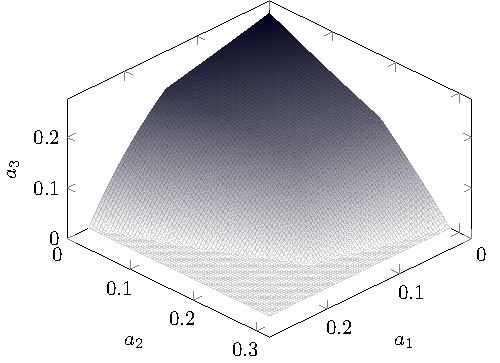
\includegraphics[width=\textwidth]{Figures/Ch7_theorem_stab.pdf}
    \else
        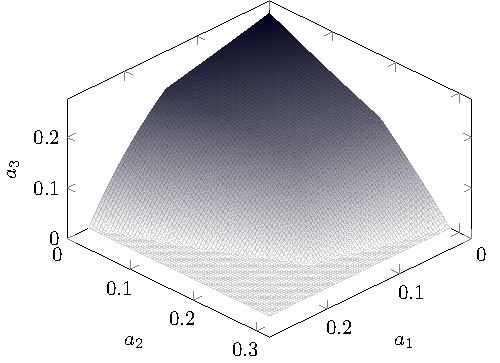
\includegraphics[draft,width=\textwidth]{Figures/Ch7_theorem_stab.pdf}
    \fi
    \caption{Stability region $\cal{R}$ according to Theorem~\ref{TH:STABILITY} for $p_1 = 1/3$, $p_2 = 2/3$, $p_3 = 1$, $\psi_1\lambda_1=1$, $\psi_2\lambda_2=2$, $\psi_3\lambda_3=3$, $\psi_1/P_1 = 1/3$, $\psi_2/P_2 = 1/2$, $\psi_3/P_3= 1$.}
\label{fig:ThStab}
\end{subfigure}%
\begin{subfigure}{.05\textwidth}
\hspace{.05\textwidth}
\end{subfigure}%
\begin{subfigure}[t]{.45\textwidth}
  \centering
    \if\printfig1
        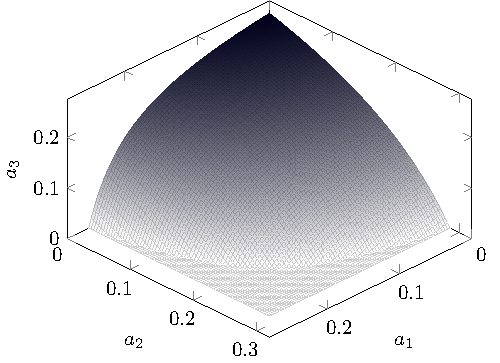
\includegraphics[width=\textwidth]{Figures/Ch7_corollary_stab.pdf}
    \else
        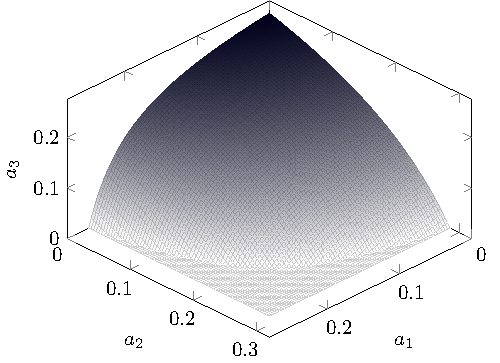
\includegraphics[draft,width=\textwidth]{Figures/Ch7_corollary_stab.pdf}
    \fi
    \caption{Maximum stability region $\cal{S}_0$ according to Corollary~\ref{cor:stab} for $p_1 = 1/3$, $p_2 = 2/3$, $p_3 = 1$,  $\psi_1\lambda_1=1$, $\psi_2\lambda_2=2$, $\psi_3\lambda_3=3$.}
\label{fig:CorStab}
\end{subfigure}
\caption{}
\end{figure}

From now on, we assume that whenever there is a packet in the buffer, the corresponding transmitter attempts to transmit, i.e., the medium access probability $p_n=1$ for all $n\in\cal{C}$.
%
We discuss in Section~\ref{sec:high-mobility} the validity of this assumption and the high-mobility assumption. The motivation is that, when the access probability of all classes is equal to one, we maximize the stability region $\cal{R}$.
%
This is easy to see with the inequalities of Theorem~\ref{TH:STABILITY}, where the right-hand side does not depend on $p_n$ and the left-hand side decreases monotonically with $p_n$. Thus, the stability region is maximized when $p_n=1$ for all $n\in\cal{C}$. The same occurs in Corollary~\ref{cor:stab}.
%
This result is surprising and might be explained by the fact that we have independence between adjacent time slots and, therefore, for each time slot there is a new scenario (a new effective PPP).
%
Then, it makes sense to always try retransmission. This approach also minimizes the mean delay according to \eqref{eq:Dn}, since the success probability $p_{s,n}$ in \eqref{eq:psn} does not depend on the access probability in a stable network.

Using Proposition \ref{prop:psk}, Proposition~\ref{prop:identity_1} is introduced, which presents an equation that relates all performance parameters independently of the transmission powers. Also, the conditions for stability are extensively simplified, see Corollary~\ref{cor:stab}.
%
\begin{proposition} \label{prop:identity_1}
	If the network is stable and $p_n=1$ for all ${n\in\cal{C}}$, then the following identities hold (at stationary state):
    \begin{equation}\label{eq:identity_1}
    	\sum_{n\in\cal{C}} \psi_n\,\lambda_n\,\dfrac{D_n}{D_n-1}\,\dfrac{a_n}{1-a_n} = 1,
    \end{equation}
    and
    \begin{equation*}
    	\frac{\psi_j}{P_j^\delta}
        \left( \frac{D_j}{D_j-1}\,\frac{1}{1-a_j} - 1\right) =
        \frac{\psi_k}{P_k^\delta} \left( \frac{D_k}{D_k-1}\,
        \frac{1}{1-a_k} - 1 \right)
        \quad \forall\,j,k\in\cal{C}.
    \end{equation*}
\end{proposition}

\begin{proof}
	We start with the terms of the sum,
	\begin{align*}
		\psi_n\,\lambda_n\,\dfrac{D_n}{D_n-1}\,\dfrac{a_n}{1-a_n}
        &\stackrel{\text{(i)}}{=} \psi_n\lambda_n\dfrac{a_n}{1-p_{s,n}}\\ 
		&= P_n^\delta \dfrac{\lambda_n\,a_n}{p_{s,n}} \left( 
        \dfrac{\psi_n}{P_n^\delta} \dfrac{p_{s,n}}{1-p_{s,n}} \right)\\
        &\stackrel{\text{(ii)}}{=} \frac{ P_n^\delta\frac{\lambda_n\,a_n}{p_{s,n}} }
        { \sum_j P_j^\delta\frac{\lambda_j\,a_j}{p_{s,j}} },
	\end{align*}
    where (i) comes from \eqref{eq:Dn} with $p_n=1$ and (ii) comes from \eqref{eq:psk_equivalence}. Summing over $\cal{C}$ ends the proof of the first identity.
    %
    For the second relation of Proposition~\ref{prop:identity_1}, we use \eqref{eq:Dn} once again to find
    \begin{equation*}
    	\dfrac{\psi_n}{P_n^\delta} \left( \dfrac{D_n}{D_n-1}\,\dfrac{1}{1-a_n} - 1\right) = \dfrac{\psi_n}{P_n^\delta} \dfrac{p_{s,n}}{1-p_{s,n}}.
    \end{equation*}
    Comparing this expression with \eqref{eq:Pi_Pk} ends the proof.
\end{proof}

Proposition~\ref{prop:identity_1} is an elegant form to see that a channel is a limited resource regarding traffic intensity and delay. Let us rewrite the identity \eqref{eq:identity_1} in terms of physical parameters,
\begin{equation} \label{eq:physical}
	\sum_{n=1}^N 4\,\lambda_n\,\overline{R}_n^2\,\theta_n^{2/\alpha}\,\dfrac{D_n}{D_n-1}\,\dfrac{a_n}{1-a_n} = \dfrac{\sin(2\pi/\alpha)}{2\pi/\alpha}.
\end{equation}
%
Note that $\frac{a_n}{1-a_n}$ and $\frac{\sin(2\pi/\alpha)}{2\pi/\alpha}$ are monotonic increasing functions and $\frac{D_n}{D_n-1}$ is a monotonic decreasing function. The right hand-side of \eqref{eq:physical} can be seen as the amount of resource available to all users of the channel.
%
Larger $\alpha$ results in higher   $\frac{\sin(2\pi/\alpha)}{2\pi/\alpha}$, meaning that a larger amount of resource is available to users. This can be explained by recalling that a larger path loss exponent leads to stronger isolation among links sharing the channel and, consequently, more users can be accommodated in the network.
%
Therefore, the larger the path loss exponent $\alpha$, the larger (smaller) the terms $\lambda_n$, $\overline{R}_n$, $\theta_n$, $a_n$ ($D_n$) can be. The identity \eqref{eq:physical} also tells us that the $n$th class of user takes a well-defined portion of the amount of resource available in the network, which is given by the $n$th term in the summation. 
%
This means that the values of $\lambda_n$, $\overline{R}_n$, $\theta_n$, $a_n$ and $D_n$ for a given class $n$ can be adjusted, while keeping the quantity $\lambda_n\,\overline{R}_n^2\,\theta_n^{2/\alpha}\,\frac{D_n}{D_n-1}\,\frac{a_n}{1-a_n}$ unchanged.
%
For instance, we can make a direct exchange between decreasing the delay $D_n$ and decreasing the arrival rate of packets $a_n$ (by controlling the ratio of transmit power levels), such that the term $\frac{D_n}{D_n-1}\,\frac{a_n}{1-a_n}$ remains constant; or else, increase the arrival rate of packets and decrease the density of users, such that the term $\lambda_n\,\frac{a_n}{1-a_n}$ remains constant. 
%
Therefore, Proposition \ref{prop:identity_1} reveals, through a simple expression, the interplay among traffic intensity, mean delay, density of users, link distance, and outage probability, when the network is stable.

\begin{remark}
    Corollary~\ref{cor:stab} and Proposition~\ref{prop:identity_1} are the simplest and the most meaningful results of the present chapter, as they translate the behavior of the network in simple equations, which do not directly depend on the transmission powers.
\end{remark}


\begin{figure}
\centering
\begin{subfigure}[t]{.45\textwidth}
  \centering
    \if\printfig1
        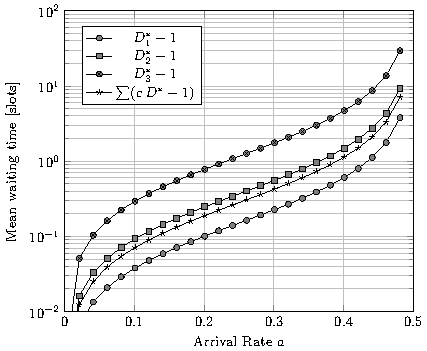
\includegraphics[width=\textwidth]{Figures/Ch7_Opt_Delay_equal_a.pdf}
    \else
        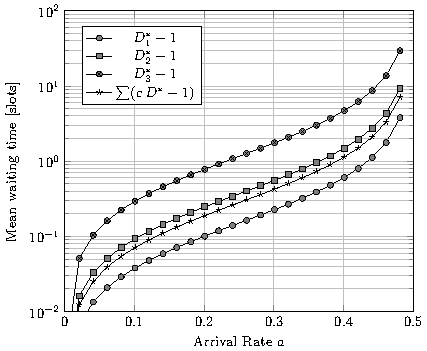
\includegraphics[draft,width=\textwidth]{Figures/Ch7_Opt_Delay_equal_a.pdf}
    \fi
    \caption{Optimum delays}
\label{fig:Opt_Delay_equal}
\end{subfigure}%
\begin{subfigure}{.05\textwidth}
\hspace{.05\textwidth}
\end{subfigure}%
\begin{subfigure}[t]{.45\textwidth}
  \centering
    \if\printfig1
        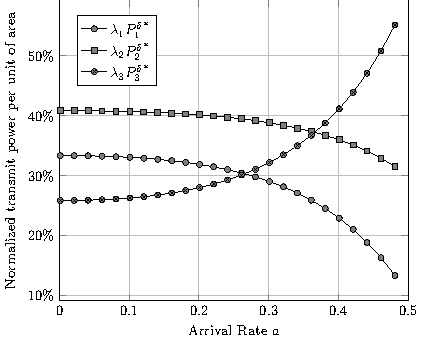
\includegraphics[width=\textwidth]{Figures/Ch7_Opt_Power_equal_a.pdf}
    \else
        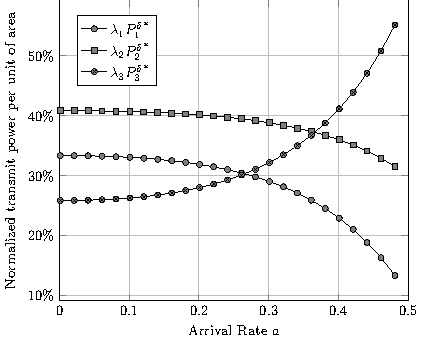
\includegraphics[draft,width=\textwidth]{Figures/Ch7_Opt_Power_equal_a.pdf}
    \fi
    \caption{Optimum transmit powers}
\label{fig:Opt_Power_equal}
\end{subfigure}
\caption{These figures represent the optimization of a 3-class network with the following parameters: $a_1=a_2=a_3=a$, $\psi_1\,\lambda_1 = 0.1$, $\psi_2\,\lambda_2 = 0.3$, $\psi_3\,\lambda_3 = 0.6$ and $c_1 = \frac{10}{16},~ c_2 = \frac{5}{16},~ c_3 = \frac{1}{16}$.}
\label{fig:opt}
\end{figure}

% % % % % % % % % % % % % % % % % % % % % % % % % % % % % %
\subsection{Interpretation and Application}
\label{sec:application}

In this section, we solve two optimization problems using the proposed formulation applied to scenarios of different classes of terminals sharing a radio channel.

% -------------------------------- %
\subsubsection{Delay Optimization}
\label{ssec:opt_delay}

Let us consider the scenario with $N$ classes sharing a channel. Each class may represent a particular user application, with each application having a different delay requirement in the network.
%
Let us suppose we are interested in adjusting the transmit power of each user class, such that the weighted average delay among all classes is minimized.
%
This problem is addressed as follows. For fixed arrival rates of vector $\bm{a}$ that satisfies Corollary~\ref{cor:stab}, i.e., for $\bm{a}\in\cal{S}_0$, let us minimize the delays $\bm{D}$ by changing the ratio between the transmit powers $\bm{P}$.
%
Each user class requires a different response time, then we weight the optimization problem with the vector $(c_1,c_2,\dots,c_N) \in \R_+^N$. The larger the coefficient of a class, the smaller the resulting mean delay to deliver packets for that class. Then, we have
\begin{equation} \label{eq:opt_prob}
	\min_{\bm{P}\in\R_+^N} \sum_{n\in\cal{C}} c_n D_n
    = \min_{\bm{P}\in\R_+^N} \sum_{n\in\cal{C}} \frac{c_n\,(1-a_n)}
        	{\left( 1 + \frac{\psi_n}{P_n^\delta}
        	\frac{\sum_j P_j^\delta\,a_j\lambda_j}
        	{1 - \sum_j \psi_j\,a_j\lambda_j} \right)^{\hspace{-1mm}-1}\!\!\! - a_n},
\end{equation}
where $D_n$ is given by Proposition~\ref{prop:psk}. Note that as thermal noise is not considered in our model, we have a degree of freedom for the optimum solution $\bm{P}^*$, which agrees with the formulation in \eqref{eq:opt_prob}.

\begin{proposition} \label{prop:opt}
	The minimum of the optimization problem \eqref{eq:opt_prob} is attained by
    \begin{equation} \label{eq:opt_D}
        {P_n^*}^\delta
        	= \dfrac{\beta}{\lambda_n a_n} \left( \frac{a_n\,\cal{A}_n}
            {1 - \sum_{k} \cal{A}_k }
            + \frac{\sqrt{c_n\,\cal{A}_n}}
            { \sum_{k} \sqrt{c_k\,\cal{A}_k } } \right), \quad n\in\cal{C},
    \end{equation}
    where $\beta$ is any positive real constant, $\cal{A}_n \triangleq \psi_n\,\lambda_n\,\frac{a_n}{1-a_n}$ and the sums are over $\cal{C}$.
\end{proposition}

\begin{proof}
	Since we have one degree of freedom for the solution $\bm{P}^*$, let us set $\sum_j P_j^\delta\,a_j\lambda_j = 1 - \sum_j \psi_j\,a_j\lambda_j$ to extensively simplify the algebraic manipulations. Then, we use the Karush-Kuhn-Tucker conditions \cite[Section~3.3.1]{bertsekas1999nonlinear} in the \emph{Lagrangian} function
    \begin{equation*}
    \begin{split}
    	\cal{L}(\bm{P},\mu) 
    	    &= \sum_{n\in\cal{C}} \frac{c_n (1-a_n)}
        	    {\left( 1 + \frac{\psi_n}{P_n^\delta}\right)^{-1}\! - a_n} + \mu\left[ \sum_{j\in\cal{C}} P_j^\delta\,a_j\lambda_j 
            	- \left(1 - \sum_{j\in\cal{C}} \psi_j\,a_j\lambda_j\right) \right],
    \end{split}
    \end{equation*}
    where $\mu\in\R$ is the \emph{Lagrange} multiplier.
    %
    The objective function is strictly convex (the Hessian is a diagonal matrix with positive eigenvalues) and the feasible region is a hyperplane, therefore the solution is the global optimum.
    %
    Now, we return to the original problem that does not have the artificial constraint. Thus, we multiply the solution by an arbitrary constant $\beta>0$ to obtain the general solution.
\end{proof}

It is interesting to note that ${\sum_k\cal{A}_k<1}$ by Corollary~\ref{cor:stab}. Therefore, ${P_n^*}^\delta$ is always a positive quantity.
%
Also, if $c_n = \cal{A}_n$ for all $n\in\cal{C}$, then the optimum delays are all equal and given by ${D_1 = D_2 = \cdots = D_N = \left( 1 - \sum_k \cal{A}_k \right)^{-1}}$. Thus, we can always choose transmit powers, such that we have the same mean delay for all classes!


As an example, let us consider a 3-class network, where Class 1 has a more restrictive delay requirement than Class 2, which is more restrictive than Class 3. We consider that all classes have the same arrival rate of packets, i.e., $a_1=a_2=a_3=a$. Figure~\ref{fig:Opt_Delay_equal} shows the expected waiting time of a packet before a successful transmission, which is $D_n^*-1$, ($n = 1,2,3$) since a transmission takes exactly one time slot. As expected, the optimization resulted in monotonic increasing functions and $D_1^* < D_2^* < D_3^*$ for all $a$.


Figure~\ref{fig:Opt_Power_equal} shows the normalized\footnote{Whenever we refer to normalized $b_n {P_n^*}^\delta$, it means that we choose $\beta$ in Proposition~\ref{prop:opt} such that $\sum_k b_k {P_k^*}^\delta = 1$ and $b_n$ is any term that depends on $n$, for example $b_n = \lambda_n$ or $b_n = a_n \lambda_n$.} transmit powers per unit of area $\lambda_n {P_n^*}^\delta$ as a function of $a$. In this case, we do not have a clear hierarchy among the transmit powers, as it depends on the traffic intensity. For $n\in\cal{C}$, if the network is close to saturation, i.e., $\sum_k\cal{A}_k$ tends to 1, then the normalized $\lambda_n {P_n^*}^\delta$ approaches $\cal{A}_n/\sum_k\cal{A}_k$ and, at first order, it does not depend on the coefficients $c_1, c_2, \dots, c_N$. On the other hand, if the network is at low traffic, i.e., $\sum_k\cal{A}_k$ tends to 0, then the normalized $a_n \lambda_n {P_n^*}^\delta$ approaches $\sqrt{c_n\cal{A}_n}/\sum_k\sqrt{c_k\cal{A}_k}$.

% -------------------------------- %
\subsubsection{Throughput Optimization}

Now, let us maximize the total throughput of the channel per unit of area with the constraint that the system is stable.
%
Since each transmitter performs retransmissions until the packet is correctly received by the intended receiver, then all packets are successfully transmitted (eventually) in a stable system. Thus, the throughput per transmitter is given by the packet arrival rate $a_n$.
%
The density of users per unit of area is given by $\lambda_n$, then the throughput of the $n$th user class per unit of area is simply $\mathscr{T}_n = \lambda_n\,a_n$ and the throughput per unit of area of the entire system $\mathscr{T}$ is the sum of the throughput for all classes $n\in\cal{C}$.

Using Corollary~\ref{cor:stab}, we can formulate the optimization problem as
${\displaystyle\max_{\bm{a}\in\cal{S}_0}} \sum_{n} \lambda_n\,a_n$.
%
However, the strict inequality in the region $\cal{S}_0$ of Corollary~\ref{cor:stab} results in an optimization problem that is not well-posed. In this case, if the optimum solution lies in the boundary of the feasible region, then the solution does not exist.
%
To circumvent this problem, we propose a new region $\cal{S}_\epsilon\subset\cal{S}_0$ by adding an arbitrarily small parameter $\epsilon \in (0,1)$ in the inequality, i.e., the new region is given by
\begin{equation*}
	\cal{S}_{\epsilon} = \left\lbrace \bm{a}\in[0,1)^N \bigm\vert \sum_{n\in\cal{C}} \psi_n\,\lambda_n\,\dfrac{a_n}{1-a_n} \le 1-\epsilon \right\rbrace.
\end{equation*}
%
As the parameter $\epsilon$ increases, the system becomes less sensitive to perturbations\footnote{When the system parameters suffer a sufficiently small change, the system remains stable.}.
Now, the optimization problem is posed as
\begin{equation} \label{eq:opt_thr}
	\max_{\bm{a}\in\cal{S}_\epsilon} \mathscr{T} = \max_{\bm{a}\in\cal{S}_\epsilon} \sum_{n\in\cal{C}} \lambda_n\,a_n.
\end{equation}
%
The following proposition presents the solution to the optimization, i.e., the optimum arrival rates $\bm{a}^*$ that maximize the throughput per unit of area and maintain the system stable.

\begin{proposition} \label{prop:eps}
	If 
    \begin{equation} \label{eq:opt_req}
		\sum_{k\in\cal{C}}\lambda_k\psi_k\left(\sqrt{\frac{\max_n \psi_n}{\psi_k}}-1\right)<1-\epsilon,
	\end{equation} then the solution of \eqref{eq:opt_thr} is attained by
    \begin{equation}
    	a_n^* = 1 - \frac{\sum_k \lambda_k \sqrt{\psi_n\psi_k}}{1-\epsilon+\sum_k\lambda_k\psi_k}, \quad n\in\cal{C},
    \end{equation}
    where the sums are over $\cal{C}$. If the inequality \eqref{eq:opt_req} is not satisfied, then the $m$th class is excluded, where $m = \arg\max_n \psi_n$, and the inequality is checked again.
\end{proposition}

\begin{proof}
	It is a direct application of the Karush-Kuhn-Tucker conditions \cite[Section~3.3.1]{bertsekas1999nonlinear} in the \emph{Lagrangian} function
    \begin{align*}
    	\cal{L}(\bm{a},\mu) = \sum_{n\in\cal{C}} \lambda_n a_n + \mu \left[ \sum_{k\in\cal{C}}\psi_k\lambda_k\frac{a_k}{1-a_k} - (1-\epsilon)\right],
    \end{align*}
    where $\mu\in\R$ is the Lagrange multiplier associated with the constraint of stability. Equation~\eqref{eq:opt_req} guarantees that the solution $\bm{a}^*\in[0,1)^N$.
    %
    The objective function is convex (affine function) and the region $\cal{S}_\epsilon$ is strictly convex because the Hessian of the function that defines the region is a diagonal matrix with negative eigenvalues. Therefore the presented solution is the global optimum and it is unique.
\end{proof}

In the optimization \eqref{eq:opt_thr}, we still have freedom to choose the transmit powers $\bm{P}$, as long the network remains stable. The best way of choosing $\bm{P}$ is by minimizing the delays, which we have already done in Subsection~\ref{ssec:opt_delay}, Proposition~\ref{prop:opt}, where the arrival rates $\bm{a} \in \cal{S}_\epsilon \subset \cal{S}_0$ are fixed. When the optimization is performed in this sequence (maximization of throughput, then minimization of delay), we have the optimum throughput (per unit of area) and the optimum delays for the optimum configuration of arrival rates.
%%
Later in this section, we illustrate this procedure with a numerical example.

In order to solve the optimization problem \eqref{eq:opt_thr} we did not have to handle with the transmit powers $\bm{P}$ directly, which would make the solution and the problem formulation more cumbersome. This shows the usefulness of Corollary~\ref{cor:stab}.

\begin{figure}
\centering
\begin{subfigure}[t]{.45\textwidth}
  \centering
    \if\printfig1
        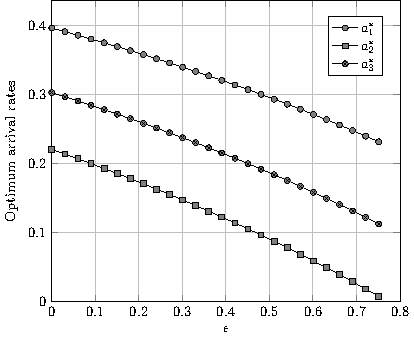
\includegraphics[width=\textwidth]{Figures/Ch7_Opt_a_eps.pdf}
    \else
        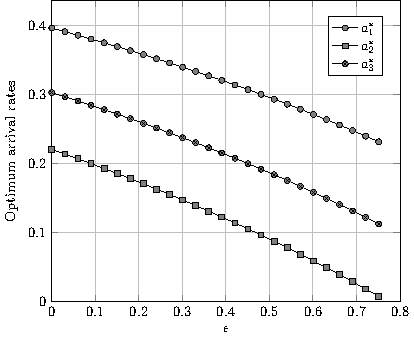
\includegraphics[draft,width=\textwidth]{Figures/Ch7_Opt_a_eps.pdf}
    \fi
    \caption{Optimum arrival rates}%
    \label{fig:Opt_a_eps}
\end{subfigure}%
\begin{subfigure}{.05\textwidth}
    \hspace{.05\textwidth}
\end{subfigure}%
\begin{subfigure}[t]{.45\textwidth}%%
  \centering
    \if\printfig1
        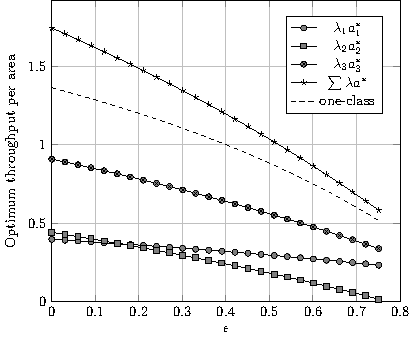
\includegraphics[width=\textwidth]{Figures/Ch7_Opt_lam_a_eps.pdf}
    \else
        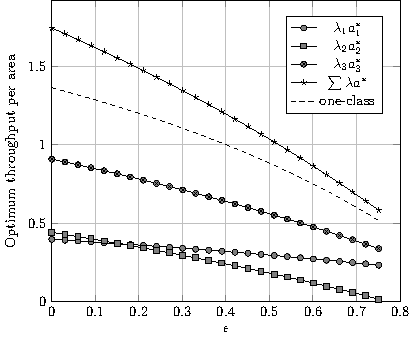
\includegraphics[draft,width=\textwidth]{Figures/Ch7_Opt_lam_a_eps.pdf}
    \fi
    \caption{Optimum throughput. The dashed curve corresponds to a scenario with only the best performing class}
    \label{fig:Opt_lam_a_eps}
\end{subfigure}
%
\begin{subfigure}[t]{.45\textwidth}%%%
  \centering
    \if\printfig1
        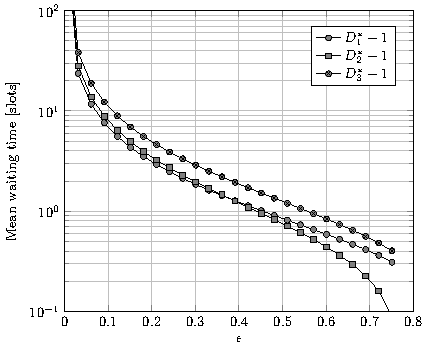
\includegraphics[width=\textwidth]{Figures/Ch7_Opt_D_eps.pdf}
    \else
        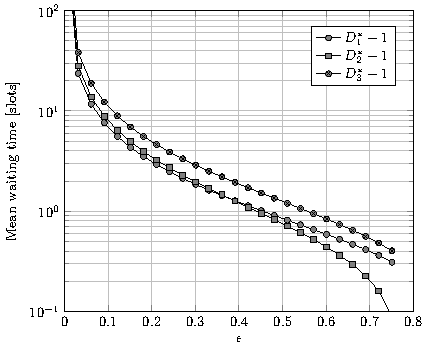
\includegraphics[draft,width=\textwidth]{Figures/Ch7_Opt_D_eps.pdf}
    \fi
    \caption{Optimum delays}
    \label{fig:Opt_D_eps}
\end{subfigure}%
\begin{subfigure}{.05\textwidth}
    \hspace{.05\textwidth}
\end{subfigure}%
\begin{subfigure}[t]{.45\textwidth}%%%%
  \centering
    \if\printfig1
        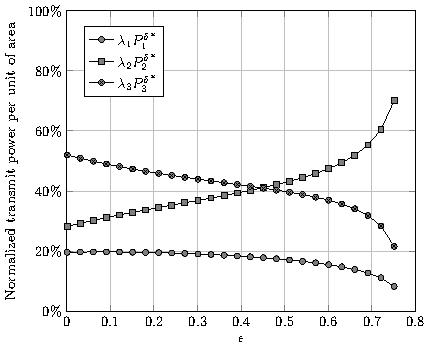
\includegraphics[width=\textwidth]{Figures/Ch7_Opt_P_eps.pdf}
    \else
        \includegraphics[draft,width=\textwidth]{Figures/Ch7_Opt_P_eps.pdf}
    \fi
    \caption{Optimum transmit powers}
    \label{fig:Opt_P_eps}
\end{subfigure}
\caption{These figures represent the optimization of the throughput and mean delay of a 3-class network with the parameters given in Table~\ref{tab:param}.}
\label{fig:opt_eps}
\end{figure}

Let us illustrate the throughput optimization problem with a system for which the parameters are shown in Table~\ref{tab:param}. Figure~\ref{fig:Opt_a_eps} shows the optimum arrival rates $\bm{a^*}$ that maximizes the throughput per unit of area.
%
\begin{table}[hbt]
  \centering
  \caption{Network parameters for Fig.~\ref{fig:opt_eps}}
  \begin{tabular}{l l}
        \hline
      \hline
      \textbf{Parameters} & \textbf{Values} \\
      \hline
        $(\lambda_1,\lambda_2,\lambda_3)$	& $=(1,2,3)$ \\
        $(\psi_1,\psi_2,\psi_3)$			& $=(0.3,0.5,0.4)$ \\
		$(c_1,c_2,c_3)$						& $=(\frac{1}{3},\frac{1}{3},\frac{1}{3})$ \\
      \hline
      \hline
  \end{tabular}
  \label{tab:param}
%   \vspace*{-\baselineskip}
\end{table}
%
It is quite interesting that the optimum solution is not (necessarily) exclusively activating the class with the best link quality (i.e., the class with the smallest $\psi$, which is Class 1 in this example). In Fig.~\ref{fig:Opt_lam_a_eps} it is shown the optimum throughput for each class and the total throughput of the system.
%
For comparison, we plotted a dashed curve representing the total throughput if we only use the best performing user class, regarding throughput.
The dashed curve is below the optimum total throughput for all $\epsilon$. Therefore, the best solution is always a combination of all user classes, as long as \eqref{eq:opt_req} is satisfied.
%
On the other hand, if this equation is not satisfied, it means that there is at least one user class with a bad link quality, such that it is better (regarding throughput efficiency) to reallocate this user class to another channel.

Now that we have, for each $\epsilon$, the arrival rate configuration $\bm{a}^*(\epsilon)$ which gives the maximum throughput, we can use Proposition~\ref{prop:opt} to find the best configuration of transmit powers $\bm{P}^*(\epsilon)$ that minimizes the sum of the mean delays for each optimum configuration of arrival rates $\bm{a}^*(\epsilon)$.
%
Figure~\ref{fig:Opt_D_eps} shows the result of this optimization, which is a direct application of \eqref{eq:opt_D}.
%
It is worth noting that as we increase $\epsilon$ the system is farther from instability, which corresponds to having a smaller delay to transmit packets, as we can see in Fig.~\ref{fig:Opt_D_eps}, and a smaller throughput, as shown in Fig.~\ref{fig:Opt_lam_a_eps}.
%
Figure~\ref{fig:Opt_P_eps} shows the optimum distribution of power per unit of area required by each user class. Notice that the first user class, which has the best link quality, uses the smallest power per unit of area. However, this behavior is more intricate; it also depends on the density of users of the corresponding class. Notice, for example, the inversion between user classes 2 and 3 as we increase $\epsilon$ in Fig.~\ref{fig:Opt_P_eps}.

Another interesting and direct result from Corollary~\ref{cor:stab} is to provide an upper bound for the total throughput per unit of area $\mathscr{T}$ in a stable system, which is given by $1/(\min_n\psi_n)$.
%
This is not a tight bound, however it is interesting on its own, due to its simplicity and the fact that it does not depend on the density of users. The proof follows
\begin{align}
	\mathscr{T} = \sum_{k\in\cal{C}} a_k\lambda_k &\le \frac{1}{\min_{n}\psi_n} \sum_{k\in\cal{C}} \psi_k\,a_k\,\lambda_k \nonumber\\
        &< \frac{1}{\min_{n}\psi_n} \sum_{k\in\cal{C}}\psi_k\,\lambda_k\,\frac{a_k}{1-a_k} \nonumber\\
        &< \left(\textstyle\min_{n}\psi_n \right)^{-1},
\end{align}
where the last inequality comes from Corollary~\ref{cor:stab}.

% % % % % % % % % % % % % % % % % % % % % % % % % % 
% % % % % % % % % % % % % % % % % % % % % % % % % % 
\section{On the High-mobility Assumption} \label{sec:high-mobility}

In this section, we address the high-mobility assumption, which may not be realistic in real wireless networks, since the mobility of transmitters does not change drastically between adjacent time slots. Therefore, the independence assumption would not hold.
%
Nevertheless, in a stable wireless network that has a small packet arrival rate $a$ per user or a small access probability $p$, the correlation might be sufficiently small such that the independence (high-mobility) assumption is reasonable. In \cite{haenggi2013diversity} the authors show that if the access probability $p$ is sufficiently small, then the independence assumption provides a good approximation.

When the packet arrival rate $a$ or the access probability $p$ are small, the typical user sees a significantly different PPP of transmitters for each time slot, which justifies the independence (high-mobility) assumption. We verified this claim through simulations and the result is shown in Fig.~\ref{fig:high-mobility}, where it is used one user class with ${\lambda c \overline{R}^2 = \pi/4}$, ${\alpha = 3}$ and ${\theta = 1}$.
%
\begin{figure}
    \centering
    \if\printfig1
        \includegraphics[width=0.55\textwidth]{Figures/Ch7_high-mobility.pdf}
    \else
        \includegraphics[draft,width=0.75\textwidth]{Figures/Ch7_high-mobility.pdf}
    \fi
    \caption{Queue load $\rho$ as a function of the access probability $p$. Simulation results with a static network are presented in marks and the theoretical results with the high-mobility assumption are presented in curves.}
    \label{fig:high-mobility}
\end{figure}

The mean load of the queues $\rho$, which is equivalent to the percentage of queues with packets to transmit, are plotted as a function of the access probability $p$ for several values of arrival rate $a$. As expected, for small values of $a$ or $p$, the theoretical model presents good estimations of the average queue load.
%
It is important to emphasize that we did not plot the mean delay $D$, because in a static PPP there might exist a set of unstable users, whose queues and delays tend to infinity. This would raise the average delay to infinity too. Then, we chose to plot the mean load $\rho$, which is equal to 1 for unstable users and does not tend to infinity opposed to the mean delay $D$.

To establish Proposition~\ref{prop:identity_1}, we supposed that the access probability $p$ is equal to one for all users. In the context of high-mobility, this approach makes sense, since the typical user sees a different interference scenario for each time slot. Thus, it is reasonable to attempt a retransmission every time slot until the packet is successfully transmitted. This also minimizes the mean delay $D$, which is in accordance with \eqref{eq:Dn}, as the transmission success probability $p_{s,n}$ does not depend on the access probability $p_n$ in a stable network.

There is another scenario, which does not require high-mobility to achieve spatial independence between adjacent time slots. This scenario is a network that uses the frequency-hopping scheme over a set of channels \cite{tse2005fundamentals}. For each time slot, there is a different PPP pattern, since the transmitting nodes select with equal probability one channel to transmit. Thus, the spatial correlation between time slots decreases with the number of channels available for selection.

% % % % % % % % % % % % % % % % % % % % % % % % % % 
% % % % % % % % % % % % % % % % % % % % % % % % % % 
\section{Bandwidth Partitioning on High-mobility Bipolar Networks}
\label{sec:bandwidth}

In this section, we consider the model presented in Section~\ref{sec:N-class} with only two classes of users, i.e., $N=2$.
%
However, differently from our previous models, the available frequency band is partitioned among users of one of the classes, such that users of this class can access only a fraction of the original bandwidth available to the network at a time.
%
The other class continues using the whole frequency band available.
%
The motivation for such bandwidth partitioning is to reduce the interference among users, leading to a higher network capacity.

The work presented in this section generalizes the paper by Jindal et al. in \cite{jindal2008bandwidth} in the sense that it (\textit{i}) considers two user classes and (\textit{ii}) investigates the effects of bandwidth partitioning on the mean \textit{queuing} delay.
%
By considering two classes of users, we are able to study the performance of a network in which users of one class are allowed to transmit on a fraction of the channel accessed by users of the other class. Also, by studying the delay, we are able to have a better understanding of the effects of bandwidth partitioning on network performance.
%
% The present work also extends the study presented in \cite{dester2018} by using bandwidth partitioning on one of the user classes. 
% More specifically, we recover some results from \cite{jindal2008bandwidth} and \cite{dester2018} by setting the arrival rate of Class 2 $a_2 = 0$ and by setting the number of band partitions $M=1$, respectively.

We used the wireless network formulation proposed in Section~\ref{sec:N-class} to achieve a tractable framework for the analysis of the bandwidth partitioning.

The main contributions presented in this section can be summarized as follows:
\begin{itemize}
    \item We have found a pair of simple equations that relate the main parameters of the network and guarantees network stability (Theorem~\ref{th:identity});
    \item A transcendental equation to find the optimum Class 1 spectral efficiency is derived, along with the optimum number of partitions (Theorem~\ref{th:optimum_eta});
    \item The first-order expansion of the optimum spectral efficiency around a small use of the channel by Class 2 (Eq.~\eqref{eq:eta_expansion});
    \item We show that the bandwidth partitioning strategy is more effective when the path loss exponent is not small and the performance requirements of Class 2, the one whose users access the whole bandwidth, is not high in respect to the maximum performance attainable (Fig.~\ref{fig:a_ratio}).
\end{itemize}

% The paper is organized as follows. In Section~\ref{sec:sysmod_M} the system model is presented and in Section~\ref{sec:stab} we derive the stability conditions and expressions for stationary transmission success probability and mean delay. Using these expressions, we present in Section~\ref{sec:opt} the optimization problem involving bandwidth partitioning and proves the existence and uniqueness of the solution.  Section~\ref{sec:num} provides some numerical examples of bandwidth optimization. %, also including a case involving cellular and D2D.
% Section~\ref{sec:conc} concludes the paper.

% % % % % % % % % % % % % % % % % % % % % % % % % % % % % %
\subsection{System Model} \label{sec:sysmod_M}

We consider the network model presented in Section~\ref{sec:N-class} with two user classes (namely Class 1 and Class 2), and only one and important difference that users of Class 1 access a fraction of the bandwidth during each transmission.

%The high-mobility model, which is used in several works (see, for instance \cite{jindal2008bandwidth}, \cite{baccelli2010stochastic}, \cite{stamatiou2010random}, \cite{dester2018}), assumes that users occupy a different point in space for each time slot. 
%The communication protocol is the slotted Aloha, i.e., for each time slot, if a source (transmitter) has packets to transmit, it will transmit one packet with a fixed probability, independently from other sources and the past. The position of source $i \in \N$ of class $n\in\{1,2\}$ at time $t\in\N$ is denoted by $X_{i,n}(t) \in \R^2$. We assume that $\{X_{i,n}(t)\}_i\subset \R^2$ is a marked homogeneous Poisson point process (PPP) of density $\lambda_n$. These PPPs are independent across classes and time slots. The transmit power of a source of class $n$ is denoted by $P_n$, assumed to be constant over time slots and the same for all sources within a class.
%
% Let $Y_{i,n}(t)\in\R^2$ be the position of the destination terminal with which the $i$th source of class $n$ communicates. The distribution of $Y_{i,n}(t)$ is such that the location of the destination terminal is at a random distance $R_{i,n}(t) = ||X_{i,n}(t) - Y_{i,n}(t)||$ from the corresponding transmitter in a uniformly random direction, where $||\cdot||$ is the euclidean norm. We assume that $R_{i,n}(t)$ is iid across time slots and users, and it follows a Rayleigh distribution of mean $\overline{R_n}$.
%
% This assumption contributes to the tractability of the model and it was also used in \cite{dester2018, lin2014spectrum, di2014stochastic}. In this context, a reasonable assumption is to consider an interference-limited network, i.e., the noise is negligible.
% It should be noted that the destination terminals are not part of the Poisson Point Processes that model the positions of the sources.

% Each source has a buffer of infinite capacity for arriving packets. The total number of packets in the $i$th source of class $n$ at time $t$ is denoted by the queue length $Q_{i,n}(t)$. If the queue of a given source is not empty, then the source tries to transmit a packet with probability $p_n$ (medium access probability) following the first-come-first-serve
% (FCFS) discipline and the transmission takes exactly one time slot.
% %
% Thus, each queue length $Q_{i,n}(t)$ forms a Markov chain (for more details, see \cite{dester2018}).
% %
% The packet is successfully transmitted when the signal-to-interference ratio (SIR) of the received signal is greater than a threshold $\theta_n$ (capture effect). In this case, the receiver sends an acknowledge through an error-free channel and the packet leaves the queue. Packets arrive at the queue according to an iid Bernoulli distribution of parameter $a_n$.
% %
% Chronologically, within each time slot, we have the transmission of packets, then the arrival of packets, and, at the end of the time slot, the displacement of the sources occurs to form a new and independent PPP realization.

% The SIR experienced by the typical user from class $n$ is given by $\mathrm{SIR}_{i,n}= P_n h_{i,n} R_{i,n}^{-\alpha}/I$, where $\alpha>2$ is the path-loss exponent, the Rayleigh fading effect is represented by the fading coefficient $h_{i,n}$, which is an iid (with respect to time and users) exponentially distributed random variable of unit mean and remains constant during the time slot, and $I$ is the aggregate interference from other sources. It is known that $\mathrm{SIR}_{i,n}$ is an iid random variable with respect to time \cite{baccelli2010stochastic}.

More specifically, the frequency band of bandwidth $B_0$ is shared by users of both classes. For Class 1 transmissions, this frequency band is divided into $M$ partitions (sub-bands) of bandwidth $B_0/M$, and each Class 1 user transmits over one randomly selected sub-band. Therefore, the density of sources for each partition becomes $\lambda_1/M$. On the other hand, users of Class 2 transmit over the whole available bandwidth $B_0$.
%
Note that front-end receiver filters of the first class destinations will capture $1/M$ of the power from transmissions of users of the second class and do not capture anything from other partitions of the first class. On the other hand, the second class destinations capture all the power coming from sources of both classes.

The transmission rate $R_T$ for the first-class users is fixed and, as in \cite{jindal2008bandwidth}, the SIR threshold\footnote{The transmission successfully happens if and only if the SIR is greater than the threshold.} $\theta_1$ comes from the following equation: ${R_T = (B_0/M)\,\ln(1+\theta_1)}$. Then, ${\theta_1 = \euler^{M\eta_0}-1}$, where ${\eta_0 \triangleq R_T/B_0}$ is the spectral efficiency without partitioning the frequency band. Note that the transmission rate for the first class of users remains unchanged with bandwidth partitioning.

% Both user classes use the same bandwidth and the goal is to find the optimum number of partitions $M$ for the first user class.
% Table~\ref{tab:symbols} summarizes the notation.

% \begin{table}[hbt]
%   \centering
%   \caption{Symbols and Definitions}
%   \begin{tabular}{ll}
%       \toprule
%       \textbf{Symbol} & \textbf{Definitions} \\
%       \midrule
%         $\alpha\in(2,\infty)$	& Path loss exponent \\
%         $\delta\in(0,1)$		& $\triangleq 2/\alpha$ \\
% 		$M \in \N$				& Number of partitions \\
%         $\eta_0 \in \R_+$		& Spectral efficiency without bandwidth partitioning \\
%         $\eta  \in \R_+$		& $\triangleq M \eta_0 $, spectral efficiency of Class 1 \\
%         $p_n\in[0,1]$   		& Medium access probability \\
%       	$a_n\in[0,1]$			& Packet arrival rate \\
%         $p_{s,n}\in[0,1]$		& Stationary transmission success probability \\
%         $\theta_n\in \R_+$		& SIR threshold for successful transmission \\
%         $D_n\in(1,\infty)$		& Average packet transmission delay \\
%         $\overline{R}_n\in \R_+$& Mean source-destination separation distance \\
%         $P_n\in \R_+$			& Transmit power \\
%         $\lambda_n\in \R_+$		& User density of class $n$\\
%         $\psi_n\in \R_+$ 		& $\triangleq 4\,\Gamma(1+\delta)\,
%          						  \Gamma(1-\delta)\,\overline{R}_n^2\,
%                                   \theta_n^{\delta}$~~(link quality)\\
% %          $||\cdot||$			& Euclidean norm \\
%         % $\ind_A(x)$				& indicator function\\
%         $\Psi_n\in \R_+$       ~& $\triangleq \psi_n\lambda_n \left(\frac{D_n}{D_n-1}\right) \left(\frac{a_n}{1-a_n}\right)$~~(resource utilization)\\
%       \bottomrule
%   \end{tabular}
%   \label{tab:symbols}
% %    \vspace*{-\baselineskip}
% \end{table}

% % % % % % % % % % % % % % % % % % % % % % % % % % % % % %
\subsection{Stability Conditions and Stationary Analysis}
\label{sec:stab}

In this section, we derive conditions for stability and carry a stationary analysis of the network, which leads to expressions relating network parameters and performance metrics. These expressions are used in Section \ref{sec:opt} to formulate an optimization problem to maximize the network performance when bandwidth partitioning is employed. 

% In order to derive the stability conditions, we first determine the successful transmission probability of a typical user from class $n\in\{1,2\}$, given the \textit{effective density of active sources} $\lambda^\mathrm{eff}_k(t)$ for each class $k\in\{1,2\}$ in a time slot $t\in\Z_+$.
% %
% The effective density of active sources of a class is the PPP density of the sources with non-empty queues and allowed by the medium access control technique to transmit a packet.
% %
% This access control is modeled in this work by the medium access probability $p_n$. One can calculate the probability of successful transmission by deconditioning the general expression for the successful probability given in \cite[Eq.~(9)]{haenggi2009stochastic} for the distance $R$, when $R$ follows a Rayleigh distribution. This was done in \cite[Proposition~1]{dester2018}. Then, the successful transmission probability is given by

From the proof of Proposition~\ref{prop:psk} in Eq.~\eqref{eq:P_SIR}, for two classes of users, we can write that%
\begin{equation} \label{eq:P_SIR_M}
	\P(\mathrm{SIR}_{i,n}(t) > \theta_n) 
    	= \nu_n\!\left( P_1^\delta\,\lambda_\mathrm{eff}^{(1)}(t)
        	+ P_2^\delta\,\lambda_\mathrm{eff}^{(2)}(t) \right), \quad t\in\N,
\end{equation}
where the function ${\nu_n: \R_+ \longrightarrow \R_+}$ is defined as
\begin{equation}\label{defNu}
\nu_n(x) \triangleq \left(1+\frac{\psi_n}{P_n^\delta}x\right)^{-1}, \quad x\in\R_+, n\in\{1,2\}.
\end{equation}

A necessary and sufficient condition for the stability of the buffers for both user classes is given by the following proposition.
%
% A system is stable whenever the Markov chain describing the system admits a proper limit distribution when $t\to\infty$ \cite{szpankowski1994stability}.
%
Stability region refers to the set of arrival rates for which the system is stable.

\begin{proposition} \label{prop:stability}
The system network is stable if and only if $(a_1,a_2) \in \mathcal{E}_1 \cup \mathcal{E}_2$, where
\begin{align*}
	\mathcal{E}_1
    	&= \left\lbrace (a_1,a_2)\in [0,1]^2 \mid
    		a_1 < p_1\,\nu_1\!\left( P_1^\delta\tfrac{\lambda_1}{M}p_1
            	+\tfrac{P_2^\delta}{M^\delta}\lambda_2 p_2\right), 
            a_2 < p_2\,\nu_2\!\left( P_1^\delta\lambda_1
        		\tfrac{a_1}{\widetilde{p}_{s,1}} + P_2^\delta\lambda_2 p_2 \right) \right\rbrace,\\
	\mathcal{E}_2
    	&= \left\lbrace (a_1,a_2)\in [0,1]^2 \mid
    		a_2 < p_2\,\nu_2\!\left( P_1^\delta\lambda_1 p_1
            	+P_2^\delta\lambda_2p_2\right), 
            a_1 < p_1\,\nu_1\!\left(P_1^\delta
        		\tfrac{\lambda_1}{M}p_1+\tfrac{P_2^\delta}{M^\delta}
                \lambda_2\tfrac{a_2}{\widetilde{p}_{s,2}} \right)
			\right\rbrace,
\end{align*}
where
\begin{equation*}
	\widetilde{p}_{s,1} = \frac{1-\psi_1\tfrac{\lambda_1}{M}a_1}
    	{1+\psi_1(\tfrac{P_2}{M P_1})^\delta\lambda_2p_2}, \qquad
    \widetilde{p}_{s,2} = \frac{1-\psi_2\lambda_2 a_2}
    	{1+\psi_2(\tfrac{P_1}{P_2})^\delta\lambda_1 p_1}.
\end{equation*}
\end{proposition}
%
\begin{proof}
	Sufficient conditions for the network stability are obtained by using the concept of dominant network \cite[Section~2.1.2]{kompella2014stable}, which corresponds to a network almost identical to the original one, differing only on the fact that users of some classes of the dominant network transmit dummy packets when their queues are empty. If the dominant network is stable, then the original network is stable as well.
	%
    Let us analyze a dominant network where both classes transmit dummy packets with the correspondent medium access probability $p_1, p_2$. In this case, the effective density of active sources for the $n$th traffic class is $\lambda_\mathrm{eff}^{(n)} = \lambda_n\,p_n$ for all $t$, since we are assuming that sources transmit dummy packets when their queues are empty.
    %
    Note that we have partitioned the frequency band of the first class of users into $M$ sub-bands, i.e., the destinations of packets of this user class only receive signals within their bandwidth, i.e., signals from $1/M$ of the sources of the first user class and $1/M$ of the power of signals the sources of the second class of users.

%    In general, a sufficient condition for stability\footnote{The system is stable if the expected rate of incoming packets is smaller than the expected number of packets leaving the queue per time slot \cite{loynes1962stability}.} for both classes are 
	A sufficient condition for stability is
    \begin{equation}
    a_n < p_n \, P(\mathrm{SIR}_{i,n} > \theta_n), \quad n\in\{1,2\},
    \end{equation}
by Loynes' theorem (Theorem~\ref{th:loynes}). Then, using Eq.~\eqref{eq:P_SIR_M}, sufficient conditions for stability for the first and the second classes are  
    \begin{equation} \label{eq:stabClass1}
    	a_1<p_1\,\nu_1\!\left[P_1^\delta\tfrac{\lambda_1}{M}p_1+\left(\tfrac{P_2}{M}\right)^\delta\lambda_2p_2\right]
    \end{equation}
    and 
    \begin{equation} \label{eq:stabClass2}
	a_2 < p_2\,\nu_2\!\left(P_1^\delta\lambda_1p_1
    	+ P_2^\delta\lambda_2p_2\right).
    \end{equation}
    If both equations \eqref{eq:stabClass1} and \eqref{eq:stabClass2} are satisfied, then the system is stable. However, the stability region described by Proposition \ref{prop:stability} can be expanded, as presented next. Let us consider two cases: (i) the arrival rate $a_1$ satisfies Eq.~\eqref{eq:stabClass1}; (ii) the arrival rate $a_2$ satisfies Eq.~\eqref{eq:stabClass2}.
\begin{enumerate}[label=(\roman*)]
    \item For this case, we consider another dominant network, where only users of the second class transmit dummy packets. We know that the first class is stable and it has a limit stationary distribution as $t\to\infty$, since we are assuming $a_1$ satisfies \eqref{eq:stabClass1}, and we want to determine a new stability condition for the second user class. We begin by noting that, in this context, the load $\rho_1$ of a queue of the first user class can be written as the ratio of the packet arrival probability and the probability a packet that leaves the queue, i.e., $\rho_1 = a_1/(p_1\widetilde{p}_{s,1})$, where $\widetilde{p}_{s,k} \triangleq \P(\mathrm{SIR}_{i,k}>\theta_k)$, $k\in\{1,2\}$, is the Class $k$ coverage probability in the dominant network. Therefore, the stationary  effective density of active sources from the first class is $\lambda_1^\mathrm{eff} = \lambda_1\,p_1\,\rho_1$. From Eq.~\eqref{eq:P_SIR_M}, we have the following fixed-point equation
    \begin{equation*}
    	\widetilde{p}_{s,1}
        	= p_1\,\nu_1\!\left[ P_1^\delta\tfrac{\lambda_1}{M}\tfrac{a_1}{\widetilde{p}_{s,1}}
            	+ \left(\tfrac{P_2}{M}\right)^\delta\!\lambda_2 p_2 \right],
    \end{equation*}
    which is easily solvable for $\widetilde{p}_{s,1}$. Then, we can use this value to derive a weaker stability condition for the second user class, i.e., $a_2<p_2\,\nu_2(P_1^\delta\lambda_1 p_1\rho_1+P_2^\delta\lambda_2 p_2)$, where $\rho_1 = a_1/(p_1\widetilde{p}_{s,1})$. This establishes the region $\cal{E}_1$.
    
    \item Analogously to case (i), we now consider a dominant network where users from the first class transmit dummy packets when their queues are empty. Following the same procedure as in the previous case, we arrive at the following fixed-point equation for the stationary successful transmission probability of the second user class,
    \begin{equation*}
    	\widetilde{p}_{s,2}
        	= p_2\,\nu_2\!\left( P_1^\delta\lambda_1 p_1
            	+ P_2^\delta\lambda_2 \tfrac{a_2}{\widetilde{p}_{s,2}} \right),
    \end{equation*}
    whose solution allows us to establish a weaker stability condition for the first class of user as
    \begin{equation}
    	a_1<p_1\,\nu_1 \left[P_1^\delta\tfrac{\lambda_1}{M}p_1+\left(\tfrac{P_2}{M}\right)^\delta\lambda_2p_2 \rho_2 \right],
    \end{equation}
    where $\rho_2 = a_2/(p_2\widetilde{p}_{s,2})$ is the load of queues from the second user class. This condition establishes region $\cal{E}_2$.
\end{enumerate}
Necessary conditions are established when we analyze the case $(a_1,a_2)\notin\cal{E}_1\cup\cal{E}_2$.
Note that, if the pair $(a_1,a_2)$ does not belong to the cases (i) or (ii), then there exists a positive probability that the original network and the dominant network, which transmits dummy packets for both classes, are \emph{indistinguishable} \cite[Section~3.2]{szpankowski1994stability} and, therefore, both systems are not stable by Loynes' Theorem (Theorem~\ref{th:loynes}). If all the queues start with a large number of packets, the original and the dominant networks behave identically with a positive probability (see \cite[Proposition~1]{stamatiou2010random}).
On the other hand, if $(a_1,a_2)$ belongs to only one of the cases (i) or (ii), then one of the classes is stable, but again with a positive probability, the original network behaves identically as the correspondent dominant network and, therefore, the other class is not stable.
\end{proof}

\begin{remark} \label{rem:stab}
The stability region in Proposition~\ref{prop:stability} is maximized when ${p_1 = p_2 = 1}$. This can be shown by noting that the two boundary inequalities that define the region $\cal{E}_1 \cup \cal{E}_2$ in the first quadrant are monotonically increasing with $p_1$ or $p_2$.
\end{remark}

Since we have established the conditions for stability, we now proceed by showing the stationary probability of successful transmission and mean delay for each user class. 

\begin{proposition}\label{prop:stationary}
	If the system is stable, then the stationary transmission success probabilities $p_{s,1}$ and $p_{s,2}$ and the stationary mean delays $D_1$ and $D_2$, for user classes 1 and 2, are given by 
\begin{gather*}
    	p_{s,1} = \frac{(1-\psi_1\tfrac{\lambda_1}{M}a_1)(1-\psi_2\lambda_2 a_2)
        	- \tfrac{1}{M^\delta}\psi_1\psi_2\lambda_1\lambda_2 a_1 a_2}
            {1+\lambda_2 a_2 \left[\psi_1\left(\tfrac{P_2}{M P_1}\right)^\delta-\psi_2\right]},\\
    	p_{s,2} = \frac{(1-\psi_1\tfrac{\lambda_1}{M}a_1)(1-\psi_2\lambda_2 a_2)
        	- \tfrac{1}{M^\delta}\psi_1\psi_2\lambda_1\lambda_2 a_1 a_2}
            {1+\lambda_1 a_1 \left[\psi_2\left(\tfrac{P_1}{P_2}\right)^\delta-\tfrac{\psi_1}{M}\right]},
     \end{gather*}  
     \begin{equation*}       
    	D_1 = \frac{1-a_1}{p_1\,p_{s,1}-a_1}, \qquad
    	D_2 = \frac{1-a_2}{p_2\,p_{s,2}-a_2}.
    \end{equation*}
\end{proposition}

\begin{proof}
	If the system is stable, then for each user class $n$, there exists the limit transmission success probability $p_{s,n}$, as $t\to \infty$. The load at a typical queue is given by $\rho_n = a_n/(p_n\,p_{s,n})$ and the effective density of active sources is $\lambda_n^\mathrm{eff}=\lambda_n p_n\rho_n$. Considering bandwidth partitioning and stationary state, we derive the following system of equations from Eq.~\eqref{eq:P_SIR_M}:
\begin{align*}
	p_{s,1} 
    	&= \nu_1\!\left[ P_1^\delta \tfrac{\lambda_1}{M} \tfrac{a_1}{p_{s,1}}
        	+\left(\tfrac{P_2}{M}\right)^\delta\!\lambda_2\tfrac{a_2}{p_{s,2}}\right],\\
	p_{s,2} 
    	&= \nu_2\!\left( P_1^\delta \lambda_1 \tfrac{a_1}{p_{s,1}}
        	+P_2^\delta \lambda_2 \tfrac{a_2}{p_{s,2}}\right),
\end{align*}
	which can be solved for $p_{s,1}$ and $p_{s,2}$. The mean delays $D_1$ and $D_2$ follow from Theorem~\ref{th:geo/geo/1} as all queues in the network can be modeled as Geo/Geo/1 queues. 
\end{proof}

Next, we provide an identity that is useful when stating the optimization problem of bandwidth partitioning in Section~\ref{sec:opt}.

\begin{theorem}\label{th:identity}
	Let $p_1=p_2=1$. The system is stable if and only if the following equations hold:
    \begin{align}
    	\frac{\Psi_1}{M} 
        	&= \frac{1-\Psi_2}{1+(M^{1-\delta}-1)\,\Psi_2}, \label{eq:theor01} \\
        \frac{P_1^\delta}{P_2^\delta}
    		&= \left(\frac{1-\Psi_2}{\Psi_1}\right) \left(\frac{\psi_1-\frac{\Psi_1}{\lambda_1 a_1}}
        		{\psi_2-\frac{\Psi_2}{\lambda_2 a_2}}\right), \label{eq:theor02} 
    \end{align}
    with $D_1, D_2 > 1$ and 
\begin{equation} \label{eq:defPsi}
\Psi_n \triangleq \psi_n\lambda_n \left(\frac{D_n}{D_n-1}\right) \left(\frac{a_n}{1-a_n}\right) \ge 0, \qquad n\in\{1,2\}.
\end{equation}    
% with $D_n\in(1,\infty)$, $n\in\{1,2\}$.
\end{theorem}

\begin{proof}
	If the system is stable, then the equations can be verified through Proposition~\ref{prop:stationary} and some manipulations. On the other hand, to prove that a set of parameters that satisfy the equations of the theorem implies stability, one can follow these steps: plug Eq.~\eqref{eq:theor02} into the inequalities of Proposition~\ref{prop:stability}; then use Eq.~\eqref{eq:theor01} and the fact that $\Psi_n > \psi_n\lambda_n\frac{a_n}{1-a_n}$ (since $\frac{D_n}{D_n-1}>1$) to show that the inequalities of Proposition~\ref{prop:stability} are satisfied. Then, the system is stable.
\end{proof}
\begin{remark} \label{rmk:Th.Stb.}
	From Theorem~\ref{th:identity},
	$\frac{\Psi_1}{M} + \Psi_2 \le 1$.
	This follows directly from equations \eqref{eq:theor01} and \eqref{eq:defPsi}.
	%
	Furthermore, for fixed $M$, the quantity $\Psi_1$ decreases if $\Psi_2$ increases. For example, let the parameters $M,\psi_1,\psi_2,a_1,a_2,D_1$, and $D_2$ be fixed; if we wish to increase the density of users $\lambda_1$ of Class 1 and maintain the aforementioned parameters constant, we necessarily need to decrease the density $\lambda_2$ of Class 2.
	%
	Note also that $\Psi_n$ increases with $a_n$ and decreases with $D_n$, such that $\Psi_n$ can be seen as a comprehensive measure of the performance of users of class $n \in \{1,2\}$.
\end{remark}

\begin{remark} \label{rmk:FreePowers}
In a network where we can freely choose the transmit power ratio $P_1/P_2$, at first we only need to satisfy Eq.~\eqref{eq:theor01} when specifying system parameters ($M,\psi_1,\psi_2,\lambda_1$,$\lambda_2$) and performance parameters ($a_1,a_2,D_1$,$D_2$). After that, we use Eq.~\eqref{eq:theor02} to specify the transmit power levels $P_1$ and $P_2$.
\end{remark}

Theorem~\ref{th:identity} considers $p_1=p_2=1$, which minimizes the mean delay for both classes (see Proposition~\ref{prop:stationary}) and maximizes the stability region (see Remark~\ref{rem:stab}). Also, if $M=1$, we recover the result in Proposition~\ref{prop:identity_1}, i.e., $\sum_n \Psi_n = 1$.

It is worth noticing the simple form through which the performance parameters $a_1,a_2,D_1$, and $D_2$ of both user classes and system stability are related.
% \textcolor{blue}{If the system does not have constraints regarding the ratio of the transmit powers, we may only use equation \eqref{eq:theor01} of Theorem~\ref{th:identity}, since it is always possible to satisfy equation \eqref{eq:theor02} in this case. Precisamos explicar melhor essa ultima sentenca}

% % % % % % % % % % % % % % % % % % % % % % % % % % % % % %
\subsection{Optimum Bandwidth Partition}
\label{sec:opt}
Let us suppose we want to maximize the performance of Class 1 users when bandwidth partitioning is employed. More specifically, for given fixed arrival rate $a_2$ and required mean delay $D_2$ of the second user class (i.e., fixed $\Psi_2$), we are interested in maximizing the quantity $\frac{\Psi_1}{\psi_1\lambda_1}=\frac{D_1}{D_1-1}\frac{a_1}{1-a_1}$, when $p_1=p_2=1$ (see Remark~\ref{rem:stab}), by adjusting the number of partitions $M$. Note that, if we set a maximum tolerable mean delay $D_1$, this choice of optimization leads to the maximum arrival rate $a_1$ admissible. On the other hand, if we fix $a_1$, this choice of optimization leads to the minimum $D_1$ achievable. From Eq. \eqref{eq:theor01} of Theorem~\ref{th:identity} and recalling that $\psi_1 = 4\,\Gamma(1+\delta) \Gamma(1-\delta) \overline{R}_1^2 \theta_1^\delta$, where $\theta_1 = \euler^{M\eta_0} - 1$, one can show with simple manipulations of the ratio $\frac{\Psi_1}{\psi_1\lambda_1}$ that maximizing the quantity $\frac{D_1}{D_1-1}\frac{a_1}{1-a_1}$ is equivalent to the following optimization problem:
%
\begin{equation} \label{eq:opt_M}
	M^* = \argmax_{M\in\N} \dfrac{M\,(\euler^{M\eta_0}-1)^{-\delta}}
    	{1+(M^{1-\delta}-1)\,\Psi_2}.
\end{equation}

% Our interest lies in finding the optimum number of bandwidth partitions $M^*$ for the first user class.
After finding the optimum number of partitions $M^*$, it is necessary to adjust the transmit power levels to satisfy Theorem~\ref{th:identity}. In this sense, we are also choosing the optimum transmit power ratio $P_1/P_2$ (see Remark~\ref{rmk:FreePowers}).

Let us now relax the constraint that $M$ must be integer to find a closed form equation for the optimization problem \eqref{eq:opt_M}, analogously to \cite{jindal2008bandwidth}. Note that after the bandwidth partition, the spectral efficiency is given by $\eta = M\eta_0$. Now, without the constraint that $M$ must be integer, we have a new goal, which is to find the optimum spectral efficiency $\eta^*$. An equivalent relaxed problem of \eqref{eq:opt_M} is
\begin{equation} \label{eq:opt_eta}
	\eta^* = \argmin_{\eta\in\R_+} \left(\euler^\eta-1\right)^\delta\,
    \left( \dfrac{1}{\eta} + \dfrac{\beta}{\eta^\delta}\right),
\end{equation}
where 
\begin{equation}
\beta \triangleq \frac{\Psi_2}{1-\Psi_2}\eta_0^{-(1-\delta)} \ge 0. 
\end{equation}
This new formulation can be obtained by taking the multiplicative inverse of the objective function in \eqref{eq:opt_M}, followed by some manipulations. The following theorem guarantees the existence and uniqueness of the optimum spectral efficiency and shows how to find it.

\begin{theorem} \label{th:optimum_eta}
	The optimum spectral efficiency $\eta^*$ is given by the unique positive solution of the following equation
\begin{equation}\label{eq:Theor02}
% 	\dfrac{h(\eta^*) - \delta}{1 - h(\eta^*)} =
%     \delta\,\beta\,{\eta^*}^{1-\delta},
	\big(1-h(\eta^*)\big) \big(1+\delta\,\beta\,{\eta^*}^{1-\delta}\big) = 1-\delta,
\end{equation}
	where $h(\eta) \triangleq (1-\euler^{-\eta})/\eta$. Furthermore, $\eta^*$ decreases monotonically with respect to $\beta$.
\end{theorem}

\begin{proof}
	Let us prove that the objective function \eqref{eq:opt_eta} is strictly convex in the region of interest. Since the sum of two strictly convex functions is strictly convex, then it is enough to show that ${[(\euler^\eta-1)/\eta]^\delta}$ and ${(\euler^\eta-1)^\delta/\eta}$ are convex with respect to $\eta > 0$. Throughout the proof we need the inequalities
    \begin{equation} \label{eq:aux_ineq}
    	0 < \euler^{-\eta} < h(\eta)^2 < h(\eta) < 1,
    \end{equation}
    which are valid when $\eta > 0$, and are easily proved using series expansion. First, let us show that
    $
    	{\frac{\partial^2}{\partial \eta^2} \left(\frac{\euler^\eta-1}
        {\eta}\right)^\delta > 0}.
    $
    For $\eta > 0$ and $\delta > 0$ and after taking the derivatives with respect to $\eta$, this inequality can be written as
	$
	{\delta\left( 1 - h(\eta) \right)^2 > \euler^{-\eta} - h(\eta)^2},
	$
which is true by \eqref{eq:aux_ineq}. Therefore, the function ${[(\euler^\eta-1)/\eta]^\delta}$ is strictly convex, since its second derivative is positive. Now, let us show that
	$
		\frac{\partial^2}{\partial \eta^2} 
        \frac{(\euler^\eta-1)^\delta}{\eta} > 0.
	$
	Again, for $\eta > 0$ and $\delta > 0$, this inequality can be written as
\begin{equation}\label{eq:der2eq}
	\delta^2 - \left(2\,h(\eta) +
    \euler^{-\eta} \right)\,\delta + 2\,h(\eta)^2 > 0.
\end{equation}
	From \eqref{eq:aux_ineq}, the inequality \eqref{eq:der2eq} is satisfied if $\delta \notin [1,2]$. Since $\alpha >2$, then $\delta\in(0,1)$, and this is enough to prove strict convexity for the function ${(\euler^\eta-1)^\delta/\eta}$ as well. Therefore, the function to be optimized is strictly convex and differentiable, i.e., if there exists a point where the derivative vanishes, then this point is unique and it is the global minimum.
    It is easy to verify that this strictly convex function is arbitrarily large when $\eta$ approaches 0 or $\infty$, then the global minimum exists and $\eta^*\in(0,\infty)$. Now, manipulating the equation 
\begin{equation*}
\frac{\partial}{\partial\eta} \left[ \left( 1 + \beta\,\eta^{1-\delta}\right)  \frac{\left(\euler^\eta-1\right)^\delta}{\eta}\right] = 0
\end{equation*}
we obtain \eqref{eq:Theor02}, concluding the proof.
The proof that $\eta^*$ decreases monotonically with respect to $\beta$ is immediate, since $h$ is a monotonically decreasing function.
\end{proof}

Figure~\ref{fig:optimum_partition} shows the optimum spectral efficiency $\eta^*$ of the first class as a function of $\beta$ for some values of the path loss exponent $\alpha$.
\begin{figure}[!t]
	\centering
	\includegraphics[]{./Figures/Ch7_optimum_partition.pdf}	
	\caption{Optimum spectral efficiency $\eta^*$ of the first class as a function of the parameter $\beta$, which is an increasing function of the parameter $\Psi_2$ of the second user class.}
	\label{fig:optimum_partition}
\end{figure}
Recall that $\beta$ is an increasing function of $\Psi_2$, which, in turn, is a comprehensive measure of the performance requirement of Class 2 users. As expected from the previous discussion, $\eta^*$ decreases as the performance requirement of the second class becomes more stringent, i.e., when $\Psi_2$ increases. This behavior of $\eta^*$ can be explained by recalling that higher spectral efficiency requires higher SIR threshold $\theta_1$, causing stronger interference to users of the second class.
%
This increased interference reduces the maximum admissible rate $a_2$ and increases the minimum achievable delay $D_2$. Since $\Psi_2$ is kept fixed in this optimization problem, $\eta^*$ must be limited. In fact, from Eq. \eqref{eq:theor01} we can see that if $\Psi_2$ increases, then $\Psi_1$ must be reduced in order to keep the system stable.
%
The propagation environment also affects the optimum spectrum efficiency. Environments with larger path loss exponent $\alpha$ reduce the interference among users, improving the channel quality and allowing for the use of higher spectral efficiency transmission schemes.

Finally, note that without the second user class ($\Psi_2 = 0$), we have $\beta=0$ and the equation for $\eta^*$ in Theorem~\ref{th:optimum_eta} has a closed form solution, which is
\begin{equation}\label{eq:opt_eff}
	\eta^*(\beta=0) = \tfrac{\alpha}{2} +
    W_0\big(-\tfrac{\alpha}{2}\,\euler^{-\alpha/2} \big),
\end{equation}
where $W_0$ is the principal branch of the Lambert-$W$ function, which is defined as the solution on $[-1,\infty)$ of the equation $W_0(x)\,\euler^{W_0(x)} = x$, for $x \ge -1/\euler$.
%
The above result is consistent with \cite[Theorem~2]{jindal2008bandwidth}, where the optimization is over the traffic density achievable and the system consists of a single user class. Expression \eqref{eq:opt_eff} was also obtained by Haenggi in \cite{Haenggi_Lambert}.

As discussed in \cite{jindal2008bandwidth}, the quantity $\delta \eta^*(0) \to 1$ as $\delta \to 0$ (i.e. $\alpha\to\infty$), which means that $\eta^*(0)$ grows asymptotically as $\alpha/2$ when the path loss exponent $\alpha$ tends to infinity.
%
However, for a given $\beta>0$, the same does not hold true. We can show that $\delta \eta^*(\beta) \to 0$ as $\delta \to 0$.

In fact, we can be more precise and show through \eqref{eq:Theor02} that if $\beta>0$, then $\sqrt{\delta} \eta^* \to 1/\sqrt{\beta}$ as $\delta\to 0$, which means that $\eta^*$ grows asymptotically as $\sqrt{\alpha/2\beta}$ when the path loss exponent $\alpha$ tends to infinity.
%
Thus, by introducing interference from another class in the system ($\beta>0$, i.e. $\Psi_2>0$), we change the asymptotic behavior of the optimal spectral efficiency from linear growth to squared root growth with respect to the path loss exponent $\alpha$.

This asymptotic result can be seen in Figure~\ref{fig:optimum_eta_delta}, where we plot the optimal spectral efficiency $\eta^*$ adjusted by the multiplicative factor $\sqrt{\beta\delta}$, which corresponds to the reciprocal of the asymptote as $\delta$ tends to $0$ (that is why all curves converge to $1$ at $\delta = 0$).
%
Another simple asymptote of $\eta^*$ is given by $2(1-\delta)/(1+\beta)$ when $\delta$ tends to $1$ (i.e. $\alpha\to2$).

\begin{figure}[!t]
	\centering
	\includegraphics[]{./Figures/Ch7_optimum_eta_delta.pdf}	
	\caption{Optimum spectral efficiency $\eta^*$ of the first class adjusted by the multiplicative factor $\sqrt{\beta\delta}$ as a function of the parameter $\delta = 2/\alpha$ for several values of $\beta$.}
	\label{fig:optimum_eta_delta}
\end{figure}

Also, we can obtain a generalization of \eqref{eq:opt_eff} when the performance requirements of Class 2 is small (i.e., $\Psi_2 \approx 0$), which is equivalent to $\beta \approx 0$. Then, we have the following first order expansion for the optimum spectral efficiency
\begin{align} \label{eq:eta_expansion}
    \frac{\eta^*\!(\beta)}{\eta^*\!(0)} = 1 - \frac{(1-\delta)\eta^*\!(0)^{1-\delta}}{\eta^*\!(0)+1-\frac{1}{\delta}} \beta + \cal{O}(\beta^2),
\end{align}
as $\beta$ tends to zero, $\eta^*\!(0)$ is given by Eq.~\eqref{eq:opt_eff} and $\cal{O}$ is the big O notation as defined in Definition~\ref{def:landau}.
% \footnote{
% We say $f(x) = \cal{O}(g(x))$ as $x\to a$, if $\limsup\limits_{x\to a} \frac{|f(x)|}{g(x)} < \infty$.
% }.
%
The above expression is found using implicit differentiation on \eqref{eq:opt_eta} and some manipulations.

We can verify through \eqref{eq:eta_expansion} that the optimal spectral efficiency has a steeper (relative) decay for larger values of the path loss exponent $\alpha$, when $\alpha > 2.48$.
%
This means that the presence of interference from another class has a larger relative impact on the optimal spectral efficiency when $\alpha$ is large.

% \begin{figure}[!t]
% 	\centering
% 	\input{./Plots/optimum_partition_norm.tex}	
% 	\caption{Optimum spectral efficiency $\eta^*$ of the first class as a function of the parameter $\beta$, which is an increasing function of the parameter $\Psi_2$ of the second user class.}
% 	\label{fig:optimum_partition_norm}
% \end{figure}

% % % % % % % % % % % % % % % % % % % % % % % % % % % % % %
\subsection{Applications}
\label{sec:num}

In this section, we illustrate the analytical results through some numerical examples. Let the first and second user classes represent the opportunist and the main users of a given bandwidth $B_0$, respectively.
%
The opportunist users access the same frequency band as the main users and we perform bandwidth partitioning for the opportunistic access in order to improve the performance of the opportunist users for a given performance of the main users, which is equivalent to fixing the quantity $\Psi_2$.

From now on, we shall use the numerical values in Table~\ref{tab:user_classes} for the numerical examples.
%
\begin{table}[!ht]
    \centering
        \caption{Parameter values.}
    \begin{tabular}{ c|l }
    \hline
    Parameters & Values \\
    \hline\hline
     $\lambda_1$        & $\SI{0.005}{/m^2}$      \\
     $\lambda_2$        & $\SI{0.002}{/m^2}$      \\
     $\overline{R}_1$   & $\SI{10}{m}$            \\
     $\overline{R}_2$   & $\SI{20}{m}$           \\
     $\eta_0$           & $\SI{0.2}{bits/s/\hertz}$   \\
     $p_1=p_2$          & $1$   \\
    \hline
    \end{tabular}
    \label{tab:user_classes}
\end{table}
%
We begin our analysis by comparing the stability regions with and without bandwidth partition. 
% Let the system parameters be $\lambda_1 = \SI{0.005}{/m^2}$, $\lambda_2 = \SI{0.002}{/m^2}$, $\overline{R}_1 = \SI{10}{m}$, $\overline{R}_2 = \SI{20}{m}$ and the (initial) spectral efficiency $\eta_0 = 0.2\,\ln(2)\,\si{nats/s/\hertz}$ for both classes.
%
Our approach to determine the stability regions is the following: we begin by using  Theorem~\ref{th:optimum_eta} to find the optimum spectral efficiency $\eta^*$ of the first class for a given value of ${\Psi_2\in(0,1)}$ (see Remark~\ref{rmk:Th.Stb.}); then, we choose the number of sub-bands $M$ as the closest integer%
\footnote{This is a functional thumb rule to find the optimum number of partitions $M^*$. However, the ideal approach is to verify through the objective function if the best is to round up or round down.
In our plots, we used the thumb rule, since there is no visual difference.}
to $\eta^*/\eta_0$ (it is worth remembering that $\Psi_2$ is fixed, so the performance requirements of Class 2 are still satisfied); finally, we use Theorem~\ref{th:identity} along with the fact that $p_1=p_2=1$ maximizes the stability region to obtain the union of the stability regions for all the transmit power ratios $P_1/P_2$ and for all medium access probabilities $p_1$ and $p_2$. The results are shown in Fig.~\ref{fig:optimum_stab_region} for $\alpha = 2.5$ and $4.5$.
%
\begin{figure}[!t]
	\centering
	\includegraphics[]{./Figures/Ch7_optimum_stab_region.pdf}%
	\caption{Stability regions of the network for different values of path loss exponent $\alpha$. The arrival rates $a_1$ and $a_2$ are the opportunist and main users, respectively; full and dashed curves correspond to the boundaries of the stability region with and without bandwidth partition, respectively. Parameter values are shown in Table~\ref{tab:user_classes}.}
	\label{fig:optimum_stab_region}
\end{figure}
%
We can see that the optimization of the spectral efficiency of the first user class (through bandwidth partitioning) expands the stability region. Note that when the path loss exponent $\alpha$ is small (close to 2), the optimization does not improve significantly the system performance.
%
Another observation is that if the traffic from main users (Class 2) is high, i.e., it is responsible for the majority of the interference, then it makes practically no difference to perform bandwidth partitioning in the opportunist class (Class 1). On the other hand, as the traffic from opportunist users increases, the impact of the optimization also increases
% \textcolor{red}{(esse melhor desempenho no canto direito inferior da região ($a_1$ alto e $a_2$ baixo) tem a ver apenas com a baixa interferência causada pelos usuários 2? Acho que poderíamos explorar esse melhor desempenho nessa região, pois é a região de interesse da ideia da partição.)}.

Let us now consider another example to analyze the effects of bandwidth partitioning on the mean delay.
% For this, we set the initial spectral efficiency for the opportunist class $\eta_0 = 0.2\,\ln(2)\,\si{nats/s/\hertz}$, the access probabilities $p_1=p_2=1$.
%
We then determine the mean delay $D_1$ of the opportunist class as a function of its arrival rate of packets $a_1$, for $\Psi_2 = 0.25, \, 0.5, \, 0.75$. Note that $\Psi_2$ can be seen here as a measure of the performance required by the main class (see Remark~\ref{rmk:Th.Stb.}). The procedure to find $M^*$ is analogous to the one used in the last example. The results are shown in Fig.~\ref{fig:optimum_delay}.
%
\begin{figure}[!t]
	\centering
	\includegraphics[]{./Figures/Ch7_optimum_delay.pdf}%
	\caption{Opportunist (first class) mean delay $D_1$ as a function of opportunist arrival rate $a_1$, for different values of the main user performance requirement $\Psi_2$. Full and dashed curves correspond to the cases with and without bandwidth partition, respectively. Parameter values are shown in Table~\ref{tab:user_classes}.}
	\label{fig:optimum_delay}
\end{figure}
%
When the performance requirements of the main users are modest (small $\Psi_2$), bandwidth partitioning allows for a more efficient use of the channel by opportunist users, i.e., a larger arrival rate $a_1$ is possible, or a smaller mean delay is achieved. On the other hand, and as expected from the previous analysis, we can also see that when the requirements of main users become more stringent (larger $\Psi_2$), then less noticeable is the improvement from the bandwidth partitioning.
%
\begin{figure}[!t]
	\centering
	\includegraphics[width=0.7\columnwidth]{./Figures/Ch7_a_ratio.pdf}%
	\caption{Maximum throughput relative improvement of Class 1 after band partition. Parameter values are shown in Table~\ref{tab:user_classes}.}
	\label{fig:a_ratio}
\end{figure}

% \begin{figure}[!t]
% 	\centering
% 	\input{./Plots/a_ratio_v2.tex}	
% 	\caption{Maximum throughput improvement of Class 1 after band partition. Parameter values are shown in Table~\ref{tab:user_classes}. \textcolor{red}{Daria para colocar ``curvas de nível'', relativas a alguns valores de ganho?}}
% 	\label{fig:a_ratio_v2}
% \end{figure}

Figure~\ref{fig:a_ratio} shows the relative improvement of the maximum throughput after band partition of Class 1 relative to the maximum throughput before band partition, for all possible values of $\Psi_2$ and $\delta$. For example, in the yellow region, we have almost doubled the throughput ($\approx 100\%$ improvement) after implementing the optimum number of band partitions. As we have previously seen through figures \ref{fig:optimum_stab_region} and \ref{fig:optimum_delay}, the bandwidth partitioning strategy of the first user class improves significantly the performance of Class 1 users as the Class 2 performance requirements $\Psi_2$ is small and the path loss exponent $\alpha$ is large (which is equivalent to small $\delta = 2/\alpha$). On the other hand, when the path loss exponent $\alpha$ is small or the performance requirements of the main (Class 2) users $\Psi_2$ is stringent, there is almost no gain in performing bandwidth partitioning of the opportunistic class (Class 1).

% % % % % % % % % % % % % % 
\section{Summary} \label{sec:summ_P2_03}

In this chapter, we derived necessary and sufficient conditions for stability in a network with $N$ user classes; we also provided simple closed form expressions for the packet success probability and mean delay. The advantage of using this model as a base to model other network effects is its analytic tractability.
%
As an example, we were able to derive simple conditions to verify the stability of an interference-limited network with undetermined transmit powers using Corollary~\ref{cor:stab}.
%
We also solved (analytically and in closed form) two optimization problems regarding the minimization of the delays in a network and maximization of the total throughput per unit of area.
%
An interesting insight from the optimization problems is that the best solution to maximize the throughput of a channel is not necessarily using solely the user class with the best link quality, i.e., a mix with other user classes may result in better use of the channel.
% 
% All in all, this paper provides a simple way to evaluate the existing trade-offs involved in the design of wireless networks when different classes of nodes co-exist.

Further, we showed that, under certain conditions, bandwidth partitioning can significantly improve the performance of the network (under stability condition) by means of higher allowable arrival rates or lower mean delays. This is the first time the problem of bandwidth partitioning is treated analytically for two interacting user classes, for which arriving packets are queued.

\chapter{Including Static Elements}
\label{cap:P2_04} \thispagestyle{empty}
\def\printfig{1} % Cap. 8
\chapterquote{%
It is the simple hypotheses of which one must be most wary; because these are the ones that have the most chances of passing unnoticed.}%
{-- Henri Poincaré, \textit{Thermodynamique} %: Leçons professées pendant le premier semestre
(1892)}

In the previous chapter, we used the high-mobility model, which assumes the node positions change drastically for each time slot.
%
A refinement of the model would be to fix some elements such that we keep analytical tractability and at the same time consider the effects of a static network.

In this chapter\footnote{The present chapter was based on the article \cite{dester2021unique}.}, we add the static element as the distance of the links, i.e., at the beginning of time, each link distance is randomized according to an arbitrary distribution and remains constant throughout time.

When including static elements, a challenge arises.
%
Each node's performance depends on its initial position, thus there might exist a set of nodes with ``bad'' positions which cause their respective queues to be unstable.
%
Thus, we cannot guarantee stability anymore, because in some systems there will be \textit{almost surely} a set of unstable nodes.
%
In these systems, it is common to use the concept of $\varepsilon$-stability \cite{zhong2016stability}. A queueing system is $\varepsilon$-stable if the system is stable except for a proportion $\varepsilon\in(0,1)$ of the queues.

The unstable queues are responsible for the Markov chain having a positive probability of never returning to a given state. This implies that we no longer have a positive recurrent Markov chain, thus we cannot guarantee ergodicity nor unicity of a stationary distribution (Theorem~\ref{th:Markov_ergodic}).
%
We explore this problem of non-unicity of the stationary distribution in $\varepsilon$-stable networks.
%
As far as we know, this is the first time this problem is tackled.

% % % % % % % % % % % % % % % % % % % % % % % % % % 
% % % % % % % % % % % % % % % % % % % % % % % % % % 
\section{On the Uniqueness of Stationary Distributions}

Considering a general path loss model and general distribution of link distances, we provide simple sufficient conditions for the uniqueness of a stationary limiting distribution.

The developed mathematical formulation guided us in finding a counterexample to a general uniqueness assumption.
%
We verified through extensive simulations that the proposed scenario indeed possesses two very different limiting stationary distributions, which remain valid even when considering a static Poisson network without the main simplifying assumptions of the original system model.

\subsection{System Model}
\label{sec:sysmod}

In view of the model presented in Chapter~\ref{cap:P2_00}, we consider a stationary static bipolar Poisson network of spatial density ${\lambda>0}$ on $\R^2$ with a single class of users. % and under slotted ALOHA protocol.
%
Time is slotted, i.e., $\T=\N$.

The distances $\{R_i(t)\}_{i\in\N}$ are defined at the first time slot independently and according to some proper distribution with an arbitrary cdf ${F_R:\R_+\longrightarrow[0,1]}$.

% Each transmitter is located at $X_i \in \Phi$, $i\in\N$, and has a dedicated receiver $Y_i$ at a fixed distance $R_i=||Y_i-X_i||$ and a uniformly distributed random direction.

% Thus, the receiver locations ${\{Y_i\}_{i\in\N} = \hat\Phi \subset \R^2}$ also form a homogeneous Poisson point process with a spatial density $\lambda$ according to the Displacement Theorem \cite[Th.~1.3.9.]{baccelli2010stochastic}.
%
%Time is slotted and denoted by $t\in\N$.

We assume unit transmit power for all users ($P_i\equiv 1$, $i\in\N$), signals subject to small-scale Rayleigh fading independent and identically distributed (iid) across space and time, and a general omnidirectional monotone decreasing path loss model ${\ell:\R_+\longrightarrow\R_+}$ that satisfies $\int_{\R_+} x\,\ell(x)\,\d x < \infty$ to guarantee that the interference is not infinite \textit{almost surely}.
%a.s.

For each transmitter $i\in\N$, packets arrive independently at its queue according to a Bernoulli point process $A_i$ on $\T$ of parameter $a\in[0,1]$, which means that $A_i(t)\sim\mathscr{B}(a)$ are iid across $t\in\T$.

The queue service discipline is general, i.e., it does not matter in which order the queued packets are transmitted because this study deals with the distribution of queued packets and not queueing delay.

If the transmitter has a nonempty queue, then it tries to transmit with an access probability $p\in[0,1]$. Thus, $T_i$ is a Bernoulli point process on $\T$ of parameter $p$.
%
We assume $a < p$, otherwise the limiting distribution is trivial with all queues being unstable \textit{almost surely}.

Packet transmissions occur in time slots with equal duration, and we assume that the Rayleigh fading coefficient is constant during this time.
%
If a packet is successfully received, then the corresponding receiver instantly sends an acknowledgment through an error-free channel and the packet is removed from the queue.

% The Signal-to-Interference Ratio\footnote{
% We assume an interference-limited network because, for the most part of large-scale networks, the effect of noise is negligible with respect to that of aggregate interference \cite{haenggi2021stochastic}.
% } at the $i$th receiver, with $i\in\N$ and associated with receiving a packet at time $t$, is computed as
% \begin{equation}
%     \SIR_i(t) = \frac{H_{ii}\,\ell(R_i)}{ \sum_{j\neq i} e_j \ind_{\{Q_j>0\}} H_{ji}\,\ell(||X_j-Y_i||) },
% \end{equation}
% where $H_{ij}$ is exponentially distributed with a parameter $1$ and represents the Rayleigh fading coefficient from transmitter $j$ to receiver $i$, $e_j\in\{0,1\}$ is iid Bernoulli distributed with a parameter $p$ and represents if user $j$ gained access to the channel, and $\ind_{\{Q_j>0\}}\in\{0,1\}$ is equal to zero if the queue of user $j$ is empty and one otherwise.

Slivnyak’s theorem (Theorem~\ref{th:slivnyak}) allows us to concentrate on the typical user, which we denote by the index $i=0$, without changing the distribution of the PPP.

Spatio-temporal correlation leads to the coupling of queues, which results in a highly complicated analysis. Thus, we assume that the interference on the typical receiver is iid across time and use the mean-field approximation \cite{kurtz1981approximation} to maintain the analytical tractability.
%
This method considers a typical queue and substitutes the interaction with other queues for an effective mean interaction, reducing the problem to the analysis of a single entity and its interdependence with the distribution of the population of entities in each state.
%
{For more details about the method applied to wireless networks, please refer to} \cite[Page~28]{haenggi2021stochastic}.

Let us assume the \textit{capture model}, where the packet from transmitter $i\in\N$ is successfully received at time slot $t\in\T$ if $\SIR_i(t)$ is greater than the threshold $\theta\in\R_+$.

Then, in a stationary network, the mean queue load of a typical user is given by
\begin{align}
    \bar\rho &= \lim_{t\to\infty} \P(Q_0(t)>0),
\end{align}
and the mean packet success probability and mean queue load of a typical transmitter with the link distance equal to $R_0$ as
\begin{align}
    p_s(R_0) &= \lim_{t\to\infty} \P(\SIR_0(t) > \theta \mid R_0),\\
    \rho(R_0) &= \lim_{t\to\infty} \P(Q_0(t) > 0 \mid R_0),
\end{align}
where $Q_0(t)\in\N$ corresponds to the number of packets in the typical queue at time $t\in\T$.

\begin{note}
    We must be careful with the definition of the network mean transmission success probability $p_s$ from Chapter~\ref{cap:P2_00}. The following calculation is not correct, in general,
    \begin{align*}
        p_s \stackrel{\times}{=} \int_{\R_+} p_s(r)\,\d F_R(r),
    \end{align*}
    because nodes with low transmission success probability transmit more times, and here we are considering only the population of nodes with each transmission distance. Instead, the correct calculation is
    \begin{align*}
        p_s = \int_{\R_+} p_s(r) \frac{\rho(r)}{\bar\rho} \,\d F_R(r),
    \end{align*}
    which weigh on the probability of the queues being non-empty.
\end{note}

% Table~\ref{tab:symbols} summarizes some definitions used in the model.
% \begin{table}[t]
%     \centering
%     \caption{Notations and symbols.}
%     \label{tab:symbols}
%     \setlength{\tabcolsep}{3pt}
%     \begin{tabular}{l l}
%       ine
%       ine
%       \textbf{Symbol} & \textbf{Definition/explanation} \\
%       ine
%         $\Z, \Z_+$				& set of integers and non-negative integers \\
%         $\R, \R_+$				& set of real numbers and non-negative reals \\
%         $\E[\cdot]$             & expected value operator \\
%         $\ind_{\{\cdot\}}$      & indicator function\\
%         $Q_i\in\Z_+$            & queue length of the $i$th user \\
%         $\ell\in\cal{C}(\R_+)$  & path-loss function \\
%         $\theta\in\R_+$         & SIR threshold for successful transmission \\
%         ine
%       ine
%     \end{tabular}
% \end{table}


% % % % % % % % % % % % % % % % % % % % % % % % % % % % % %

\subsection{Stationary Analysis}
\label{sec:stat}

At first, let us suppose that the limiting distribution exists and the mean queue load converges to $\bar\rho \in [0,1]$.
%
Then, at stationary conditions, the active transmitters form a thinned point process $\Phi^{p\bar\rho}_\TX$ from $\Phi_\TX$. Thus, it consists of a PPP of density $\lambda\,p\,\bar\rho$.
%
From Proposition~\ref{prop:PPP_ps}, the packet success probability of a typical link with a transmission distance $r > 0$ is given by 
\begin{align} \label{eq:p_s}
    p_s(r) = \exp\left(- g_\ell(r,\theta)\,\lambda\,p\,\bar\rho \right),
\end{align}
where \vspace{-2mm}
$$\displaystyle g_\ell(r,\theta) \triangleq \int_{\R_+}\frac{2\pi \, x\, \theta \ell(x)}{\ell(r)+\theta \ell(x)}\, \d x,$$
which is a strictly monotone increasing function on the first argument and tends to infinity in the positive infinity, because $\ell$ is a strictly monotone decreasing function and tends to zero in the positive infinity.
%
For ease of notation, let us omit the second argument of $g_\ell$, i.e., $g_\ell(r,\theta) = g_\ell(r)$, since $\theta$ is a constant.

Then, from Queueing theory, the stationary queue load of a typical user with the link distance $r > 0$ is
\begin{align}\label{eq:rho_r}
    \rho(r) = \min\left\{ \frac{a}{p\,p_s(r)}, 1 \right\},
\end{align}
because the service rate is given by $p\,p_s(r)$.
%
% If $\rho(r) = 1$ for some $r>0$, it means there is not stability for any typical queue with link distance greater than $r$.
However, to calculate $p_s(r)$ in \eqref{eq:p_s} we need the density of active users $\lambda_a$, which depends on the mean queue load $\bar\rho$. This, in turn, depends on $\rho(r)$. The following proposition provides a solution to this problem.

\begin{proposition}\label{prop:fixed_point}
    If the stationary mean queue load $\bar\rho\in[0,1]$ exists, it must satisfy the fixed point equation $\varphi(\bar\rho) = \bar\rho$, where
    \begin{align}\label{eq:fixed_point}
        \varphi(x) \triangleq 1 - \frac{a}{p} \int_0^{\ln(p/a)} \hspace{-7mm} \euler^u\,F_*(u/px)\,\d u, \quad x\in(0,1],
    \end{align}
    $\varphi(0)=a/p$, and $F_*$ is the CDF of the random variable $\lambda g_\ell(R)$.
\end{proposition}
%
\begin{proof}
    Using \eqref{eq:p_s}, \eqref{eq:rho_r}, integration by parts, and the substitution ${u = p\bar\rho w}$, we have
    \begin{align*}
        \bar\rho &= \E\left[\rho(R_0)\right] 
            = \E\!\left[\min\left\{ \frac{a}{p}\euler^{\lambda g_\ell(R_0) p \bar\rho}, 1 \right\} \right] \\
            &= 1 - F_*\!\left(\frac{\ln(p/a)}{p\bar\rho}\right) + \frac{a}{p} \int_0^{\ln(p/a)/p\bar\rho} \hspace{-12mm} \euler^{p\bar\rho w}\,\d F_*(w) \\
            &= 1 - \frac{a}{p} \int_0^{\ln(p/a)} \hspace{-7mm} \euler^u\,F_*(u/p\bar\rho)\,\d u = \varphi(\bar\rho),
    \end{align*}
    where $\d F(w)$ is the Lebesgue--Stieltjes notation, and if the probability density function exists we can write it as $F'(w) \d w$.
    
    Further, $\varphi(x) \to a/p$ as $x\to 0^+$, because $F_*(y) \to 1$ as $y \to \infty$, which comes from $R$ being a proper random variable.
\end{proof}

Because $g_\ell$ is strictly monotone, it is invertible, and then
\begin{align}\label{eq:F_*}
    F_*(x) =
    \begin{cases}
        F_{R}\!\left(g_\ell^{-1}\!\left(\frac{x}{\lambda}\right)\right), & \text{if } x > \lambda \displaystyle\lim_{r\to 0^+} g_\ell(r),\\
        0, &\text{otherwise}.
    \end{cases}
\end{align}

\begin{remark}
    We are dealing with a general path loss function $\ell$ and a general distribution $F_R$ of link distances, so care must be taken with $F_*$, in the sense that this function may not be sufficiently ``smooth''.
\end{remark}

Now we present some theorems that provide results on the existence and uniqueness of a valid stationary mean queue load $\bar\rho$.
%
However, before proving the theorems we need a result on the continuity of the function $\varphi$, which is defined in Proposition~\ref{prop:fixed_point} and whose fixed point provides the mean queue load of the queueing network.

\begin{lemma} \label{lem:lipschitz}
    The function $\varphi$ is $c$-Lipschitz continuous\footnote{A function $\varphi$ is $c$-Lipschitz continuous if $|\varphi(x)-\varphi(y)|\le c\,|x-y|$ for all $x,y$ in the interval.} on $[a/p,1]$ with $c = \frac{p}{a}\ln(\frac{p}{a})$.
\end{lemma}
%
\begin{proof}
    Let us prove that for all $x,y\in[\frac{a}{p},1]$, $|\varphi(x)-\varphi(y)| \le c\,|x-y|$.

    Without loss of generality let $x < y$, then
    \begin{align*}
        |\varphi(x)-\varphi(y)| &= \frac{a}{p} \left( \int_0^{\ln(p/a)} \hspace{-10mm} \euler^u F_*(u/px) \d u - \int_0^{\ln(p/a)}\hspace{-10mm} \euler^u F_*(u/py) \d u \right)\\
            &\stackrel{(i)}{=} a \left( \int_{\ln(p/a)/py}^{\ln(p/a)/px}\hspace{-14mm} x\euler^{p x w} F_*(w) \d w -  \int_0^{\ln(p/a)/py}\hspace{-14mm} (y\euler^{p y w} - x\euler^{p x w})F_*(w) \d w \right) \\
            &\le a \int_{\ln(p/a)/py}^{\ln(p/a)/px}\hspace{-12mm} x\euler^{p x w} \d w = 1 - \euler^{-\ln(p/a)\frac{y - x}{y}} \le \frac{\ln(p/a)}{y} (y - x) \\
            &\le \frac{\ln(p/a)}{a/p} |x-y|.
    \end{align*}
    In $(i)$ we perform the change of variables $u = (px)w$ for the left integral and $u = (py)w$ for the right one, and split the intervals of integration of the left integral.
\end{proof}

\begin{theorem} \label{th:existence}
    The function $\varphi$ has a fixed point on $[a/p,1]$.
\end{theorem}
\begin{proof}
    From Lemma~\ref{lem:lipschitz}, $\varphi$ is continuous because Lipschitz continuity implies continuity.
    %
    Further, $\varphi(0) = a/p < 1$ and $a/p \le \varphi(1) \le 1$.
    %
    Then, the result follows from the intermediate value theorem (Theorem~\ref{th:IVT}) applied on $\varphi(x)-x$, $x\in[a/p,1]$.
\end{proof}

\begin{theorem} \label{th:unique_sol1}
    If $a > p\,\Omega$, where $\Omega$ is the solution of $\Omega\,\euler^\Omega=1$, then the function $\varphi$ admits a unique fixed point.
\end{theorem}
%
\begin{proof}
    Using the Banach fixed point theorem (Theorem~\ref{th:banach}) along with Lemma~\ref{lem:lipschitz}, we have that $\varphi$ admits a unique fixed point if $c = \frac{p}{a}\ln(\frac{p}{a}) \in [0,1)$.
    
    This happens if $\frac{a}{p}\exp(\frac{a}{p}) > 1$ which is equivalent to $\frac{a}{p} > \Omega$.
\end{proof}

\begin{theorem} \label{th:unique_sol2}
    If $F_*$ is continuously differentiable and $a > p/\euler$, then the function $\varphi$ admits a unique fixed point.
\end{theorem}
%
\begin{proof}
    Let $\bar\rho$ be a solution to $\varphi(\bar\rho) = \bar\rho$. Then,
    \begin{align*}
        \varphi'(\bar\rho) &= \frac{a}{(p\bar\rho)^2} \int_0^{\ln(p/a)} \hspace{-7mm} u\,\euler^u\,F_*'(u/p \bar\rho)\,\d u \\
            &= \frac{1}{\bar\rho}\bigg( \ln(p/a) F_*(\ln(p/a)/p\bar\rho) - \frac{a}{p}\int_0^{\ln(p/a)}\hspace{-7mm} (1+u) \euler^u F_*(u/p\bar\rho)\,\d u \bigg)\\
            &\le \frac{\ln(p/a) - (1-\varphi(\bar\rho))}{\bar\rho} < \frac{\varphi(\bar\rho)}{\bar\rho} = 1,
    \end{align*}
    where we used the Leibniz integral rule (Theorem~\ref{th:leibniz}) to interchange the integral with the derivative to establish the first equality, then used integration by parts in the second equality.
    %
    As $\varphi$ is a continuous function and $(\varphi(x)-x)'|_{x=\bar\rho} < 0$, the fixed point equation cannot have more than one root, because $\varphi(x)-x$ always crosses the $x$-axis downwards.
\end{proof}

Since $\Omega > 1/\euler$, Theorems \ref{th:unique_sol1} and \ref{th:unique_sol2} complement each other. While one has a larger set of valid functions, the other has a larger set of arrival rates that guarantee uniqueness.

{Remarkably, we do not need any information about the distribution of the link distances, the path loss model, the threshold for successful communication, or the density of users to guarantee uniqueness through Theorems} \ref{th:unique_sol1} and \ref{th:unique_sol2} (except for $F_*$ being differentiable in Theorem~3).

Let $\varepsilon$ represent the proportion of unstable queues\footnote{In the literature \cite{zhong2016stability}, it is common to define the $\varepsilon$-stability region. However, in the present work, it is more convenient to simply define $\varepsilon$.} in the network, then in view of the mean-field approximation and Loynes theorem (Theorem~\ref{th:loynes}) we can define
\begin{align}
    \varepsilon \triangleq \lim_{t\to\infty} \P\big( p\,\P(\SIR_0(t) < \theta \mid R_0) < a \big).
\end{align}

Then, using \eqref{eq:p_s}, \eqref{eq:F_*}, and Proposition~\ref{prop:fixed_point}, we can show that
\begin{align} \label{eq:eps}
    \varepsilon &= 1 - F_* \!\left(\frac{\ln(p/a)}{p\,\bar\rho}\right)
        \le \bar\rho.
\end{align}
This inequality is expected because $\varepsilon$ takes into account only queues with load equal to $1$.

\begin{proposition}\label{prop:p_opt}
    If $F_*$ is continuously differentiable and $a > p/\euler$, then \[\dfrac{\partial\bar\rho}{\partial p} < 0 \quad\text{and}\quad \dfrac{\partial\varepsilon}{\partial p} < 0.\]
\end{proposition}
%
\begin{proof}
    Taking the derivative with respect to $p$ on both sides of the fixed point equation $\varphi(\bar\rho)=\bar\rho$ and after some tedious manipulations we have
    \begin{align} \label{eq:drho/dp}
        \frac{p}{\bar\rho} \frac{\partial\bar\rho}{\partial p}
            &= - \frac{(1-\ln(p/a))F_*(\Upsilon)+A}{1-\ln(p/a)F_*(\Upsilon) + A},
    \end{align}%
    where $\displaystyle A \triangleq \frac{a}{p}\int_0^{\ln(p/a)} \hspace{-7mm} u\, \euler^u F_*(u/p\bar\rho) \,\d u \ge 0$ and $\displaystyle \Upsilon \triangleq \frac{\ln(p/a)}{p\bar\rho}$.
    
    Since $a>p/\euler$, then $\ln(p/a) < 1$. Using this, it is easy to see that both the numerator and denominator of \eqref{eq:drho/dp} are positive. Thus, $\frac{\partial\bar\rho}{\partial p} < 0$.
    
    Note that $\varepsilon$ monotonically decreases with $\Upsilon$ from \eqref{eq:eps}. Then, let us calculate the derivative of $\Upsilon$ with \eqref{eq:drho/dp}. After some tedious manipulations,
    \begin{align*}
        \frac{p}{\Upsilon}\frac{\partial\Upsilon}{\partial p} 
            &= \frac{1}{\ln(p/a)}\,\frac{1 - \ln(p/a)+A}{1 - \ln(p/a) F_*(\Upsilon) + A}.
    \end{align*}%
    Again, it is easy to see that both the numerator and the denominator are positive. Thus, $\frac{\partial\Upsilon}{\partial p} > 0$ and $\frac{\partial\varepsilon}{\partial p} < 0$.
\end{proof}

From the above proposition, if $a \ge 1/\euler$, then the access probability $p$ that minimizes the proportion of unstable nodes and the load on the queues is $p=1$. Other works \cite{haenggi2018soc, dester2018} also reached an equivalent result in a different framework.
%
This appears to be a powerful theoretical result because it is valid for almost any set of system parameters, general path loss model, and general distribution of link distances.
%
However, we must remember that one of the model assumptions is PPP independence of the location of active transmitters across time slots, and this assumption becomes less valid as we increase the value of $p$ \cite{haenggi2013diversity}.
%
Thus, a more sensible conclusion is that, instead of setting $p=1$, we should increase $p$ as long as the system model assumptions remain valid.
%
Section~\ref{sec:counter-example} presents more material on this topic.

Now, let us turn our attention to the scenarios that have multiple limiting distributions, i.e. when $\varphi$ admits more than one fixed point.
%
We can build a sequence that converges to the least or the greatest solution of the fixed point equation, depending on the initial conditions. Let the recurrence equation that defines the sequence $\{\bar\rho_n\}_{n\in\N}$ be
$
    {\bar\rho_{n+1} = \varphi(\bar\rho_n), n\in\N}.
$
\begin{proposition} \label{prop:sequence}
    When $\bar\rho_0 = 0$, the sequence $\{\bar\rho_n\}_{n\in\N}$ converges to the least solution of $\varphi(\bar\rho)=\bar\rho$. Otherwise, if ${\bar\rho_0 = 1}$, it converges to the greatest solution.
\end{proposition}
%
\begin{proof}
    The function $\varphi$ is monotonic increasing because $F_*$ is a monotonic increasing function.
    %
    Also, $0 \le \varphi(0)$, then
    \begin{align*}
        \varphi(0) \le \varphi(\varphi(0)) \le \dots \le \varphi^n(0) \triangleq \varphi^{n-1}(\varphi(0)).
    \end{align*}
    
    Hence, when $\bar\rho_0 = 0$, the sequence $\{\bar\rho_n\}_n$ is increasing.
    %
    Clearly, it is also limited, and thus, it converges \cite[Th.~3.14.]{rudin1976principles}.
    
    Let $x = \varphi(x)$ be a fixed point. We have that $0 \le x$, then $\varphi(0) \le \varphi(x) = x$. Repeating $n$ times we get $\varphi^n(0) \le x$.
    %
    As $n\to\infty$ we know $\varphi^n(0) = \bar\rho_n$ converges, thus it converges to a value smaller or equal to $x$. But $x$ is an arbitrary fixed point. This concludes the proof for $\bar\rho_0=0$.
    %
    The proof when $\bar\rho_0=1$ is analogous.
\end{proof}

Note that the fixed point is unique if and only if the greatest solution is equal to the least solution.
%
This is a simple form to verify whether the stationary distribution is unique when neither of the uniqueness theorems (\ref{th:unique_sol1} and \ref{th:unique_sol2}) are satisfied.

Using the concept of dominant networks \cite{ephremides1988stability}, we can build a physical interpretation of Proposition~\ref{prop:sequence}.
%
Suppose a dominant network where all nodes transmit \textit{dummy} packets. The density of active transmitters is $\lambda p$, and thus, we can calculate the typical queue distributions to find the mean queue load, which we shall denote by $\bar\rho_1$. This value can be used as an upper bound to the density of active transmitters in the original network. Then, we can define a new dominant network, whose density of active transmitters is given by $\lambda p \bar\rho_1$ and find the corresponding $\bar\rho_2$, and so on. The process described above is equivalent to calculating $\bar\rho_{n+1} = \varphi(\bar\rho_n)$ with $\bar\rho_0 = 1$.
%
We can also perform an analogous reasoning for the lower bound, i.e., we assume that the density of active users is $\lambda a$, which corresponds to a system operating with a packet success probability equal to $1$, and calculate the typical mean queue load in this network, which again we shall denote by $\bar\rho_1$. This can be used to estimate another lower bound on the density of active users in the original network, and the process continues analogously to the upper bound case with the sole difference that $\bar\rho_0 = a/p$.

% % % % % % % % % % % % % % % % % % % % % % % % % % % % % %
%\section{A counter-example}
\section{Example of a non-unique stationary distribution}
\label{sec:counter-example}

Here we present a scenario where the conditions of the uniqueness theorems are not satisfied and there is more than one solution to the fixed point equation $\varphi(\bar\rho) = \bar\rho$.

As commonly chosen in the literature \cite{haenggi2021stochastic}, let the path loss function be $\ell(r) = r^{-\alpha}$, where $\alpha>2$, the distribution of $R$ be Rayleigh with mean $\mu_R$, and let us define the auxiliary parameters $\kappa \triangleq \frac{\sin(\delta\pi)}{4 \lambda \theta^\delta \delta \pi \mu_R^2}$, $\delta\triangleq 2/\alpha$. Then, ${F_*(x) = 1-\euler^{-\kappa x}}$ and for $x>0$,
\begin{align}
    \varphi(x) &= 
    \begin{cases}
        \frac{\left(\frac{a}{p}\right)\frac{\kappa}{px}-\left(\frac{a}{p}\right)^{\frac{\kappa}{px}}}{\frac{\kappa}{px}-1},\quad \text{if } x \neq \kappa/p,\\
        \frac{a}{p} \left(1 + \ln\!\left(\frac{p}{a}\right)\right), \quad\text{otherwise.}
    \end{cases}
\end{align}

For the simulations we set $a = 0.002$ packets per time slot per node, $p = 0.1$, $\lambda = 1$ node per unit of area, ${\alpha = 5}$, $\theta = 2$, $\mu_R = 3.457$ units of length, which gives a $\kappa \approx 0.012$.
%
{However, any combination of parameters that results in $\kappa < 0.248$ would work, because in this case, we can find $a$ and $p$ that give non-unicity of the fixed point, as long as $\alpha>2$.
%
Nevertheless, when $\alpha$ approaches $2$ the simulations become expensive because we need to increase the number of nodes to properly simulate the large-scale network effect.}
%
The simulations are of static Poisson networks and do not consider the simplifying assumptions of the system model, such as mean-field approximation or independence of the $\SIR$ across time and space.

\begin{figure}[ht]
    \centering
    \if\printfig1
        % 
\begin{tikzpicture}[scale=1.0]

\begin{axis}
[
  title={},
  width  = 0.8*0.8*\columnwidth,
  height = 0.8*0.4*\columnwidth,
  axis lines=center,
  legend style={at={(0.95,0.95)}, anchor=north east},
%   xmode=log,
  xlabel={$x$},
  ylabel={$\varphi(x)-x$}, ylabel style={rotate=0},
%  yticklabel=\pgfmathprintnumber{\tick}\\ \%,
  xmin = 0.0, 	
  xmax = 0.6,
%   ymin = -0.05,
%   ymax = 0.05,
  scaled y ticks = false,
  yticklabels={,,},
%   y tick label style={
%         /pgf/number format/.cd,
%         fixed,
%         fixed zerofill,
%         precision=2,
%         /tikz/.cd
%   },
  x tick label style={
        /pgf/number format/.cd,
        fixed,
        fixed zerofill,
        precision=2,
        /tikz/.cd
  },
%   grid = both,
  scale only axis,
]
	\legend{}
    
    \def\k{0.012}
    \def\p{0.100}
    \foreach \a in {0.002}
        \addplot[thick, domain = 0:0.585, samples=100] {(\k*(\a/\p)-\p*x*(\a/\p)^(\k/(\p*x)))/(\k-\p*x)-x};
    
    \fill[color = red]  (axis cs: 0.02539, 0) circle[radius=2pt];
    \fill[color = blue] (axis cs: 0.17750, 0) circle[radius=2pt];
    \fill[color = red]  (axis cs: 0.52286, 0) circle[radius=2pt];
    
    % \foreach \a in {0.1,0.2,0.3,0.4,0.5,0.555,0.62}
    %     \addplot[domain = 0:1, samples=100] {(k*(a/p)-p*x*(a/p)^(k/(p*x)))/(k-p*x)-x};
    
    % \addplot[domain = 0.5:1.04, dashed, samples=100] {x*(1+((-3 + 2*x + sqrt(5 + 4*(-1 + x)*x))/(2*x))*x)*exp(-(2-((-3 + 2*x + sqrt(5 + 4*(-1 + x)*x))/(2*x)))*x)};
    
%     \addplot[thick] table
%     [
% 		x expr = \thisrow{lam},
%     	y expr = \thisrow{25dB}
%     ] {./Data/envelopes.dat};

    % \draw[-\arrowhead] (axis cs: 0.8,0.08) -- (axis cs: 2.7,0.27) node[anchor=south west] 
    %     {$\alpha = 0.1,0.2,0.3,0.4,0.5,0.56,0.62$};
\end{axis}

\end{tikzpicture}

        \includegraphics[]{Figures/Ch8_fixed_point.pdf}
    \else
        \includegraphics[draft,width=\textwidth]{Figures/placeholder.png}
    \fi
    % \includegraphics[width=\columnwidth]{Figures/main-figure0.eps}
    \caption{Red dots are the \textit{attractors} and the blue point is the \textit{repeller}.}
    \label{fig:fixed_point}
\end{figure}

We show in Fig.~\ref{fig:fixed_point} the \textit{attractors} and \textit{repellers}
% \footnote{
% We define \textit{attractor} as a fixed point $x_a$ of $\varphi$ that satisfies $\varphi^n(x)\to x_a$ as $n\to\infty$ for all $x$ in some neighborhood $V_a$ of $x_a$, where $\varphi^n$ denotes repeated composition of the function with itself.
% %
% This neighborhood $V_a$ is called \textit{basin of attraction}.
% %
% A fixed point $x_r$ of $\varphi$ is a \textit{repeller} if there exist $n_0\in\N$ and a neighborhood $V_r$ of $x_r$ such that $\varphi^n(x)\notin V_r$ for all $n > n_0, x\in V_r\backslash\{x_r\}$.
% }
of the chosen scenario, which can be intuitively seen as ``stable'' and ``unstable'' equilibrium points, respectively.
%
The formal definition follows.

\begin{definition}
    A fixed point $x_0$ of a function $\varphi$ is an \textit{attractor} if for all $x$ in some \textit{neighbourhood}\footnote{\textit{Neighborhood} is defined in Definition~\ref{def:neighborhood}.} of $x_0$ we have that $\varphi^n(x) \to x_0$ as $n\to\infty$, where $\varphi^n(x)\triangleq \varphi^{n-1}(\varphi(x))$.
    %
    A \textit{neighbourhood} that satisfies the aforementioned property is a \textit{basin of attraction} for $x_0$.
    
    On the other hand, $x_0$ is a \textit{repeller} if there exists a \textit{neighbourhood} $V$ of $x_0$ and an integer $n_0$ such that for all $x\in V\backslash\{x_0\}$ we have that $\varphi^n(x) \notin V$ for all $n > n_0$.
\end{definition}

\begin{figure}[H]
    \centering
    \if\printfig1
        % 
\begin{tikzpicture}[scale=1.0]

\begin{axis}
[
  title={},
  width  = 0.8*0.8*\columnwidth, 
  height = 0.8*0.5*\columnwidth,
%   axis lines=center,
  legend style={at={(0.95,0.95)}, anchor=north east},
%   xmode=log,
  xlabel={Time slot $t$},
  ylabel={$\bar\rho$}, ylabel style={rotate=-90},
%  yticklabel=\pgfmathprintnumber{\tick}\\ \%,
  xmin = 0, 	
  xmax = 5000,
  ymin = 0.0,
  ymax = 0.65,
  x tick label style={
        /pgf/number format/.cd,
        fixed,
        fixed zerofill,
        precision=0,
        set thousands separator={},
        /tikz/.cd
  },
  grid = both,
  scale only axis,
]
	\legend{}
    
    % \foreach \a in {0.1,0.2,0.3,0.4,0.5,0.555,0.62}
    %     \addplot[domain = 0:1, samples=100] {(k*(a/p)-p*x*(a/p)^(k/(p*x)))/(k-p*x)-x};
    
    % \addplot[domain = 0.5:1.04, dashed, samples=100] {x*(1+((-3 + 2*x + sqrt(5 + 4*(-1 + x)*x))/(2*x))*x)*exp(-(2-((-3 + 2*x + sqrt(5 + 4*(-1 + x)*x))/(2*x)))*x)};

    \addplot[blue!50!black, each nth point=5] table
    [
		x expr = \thisrow{t},
    	y expr = \thisrow{rho1}
    ] {./Data/sim_fixed_point.dat};

    \addplot[green!70!black, each nth point=5] table
    [
		x expr = \thisrow{t},
    	y expr = \thisrow{rho2}
    ] {./Data/sim_fixed_point.dat};
    
    \addplot[brown, each nth point=5] table
    [
		x expr = \thisrow{t},
    	y expr = \thisrow{rho3}
    ] {./Data/sim_fixed_point.dat};
    
    \addplot[magenta, each nth point=5] table
    [
		x expr = \thisrow{t},
    	y expr = \thisrow{rho4}
    ] {./Data/sim_fixed_point.dat};

    \addplot[red,  line width=1.5pt, domain = 0:5000, samples=2] {0.02539};
    \addplot[red,  line width=1.5pt, domain = 0:5000, samples=2] {0.52286};
    \addplot[blue, line width=1.5pt, domain = 0:5000, samples=2] {0.17750};

    % \draw[-\arrowhead] (axis cs: 0.8,0.08) -- (axis cs: 2.7,0.27) node[anchor=south west] 
    %     {$\alpha = 0.1,0.2,0.3,0.4,0.5,0.56,0.62$};
\end{axis}

\end{tikzpicture}
%
        \includegraphics[]{Figures/Ch8_sim_fixed_point.pdf}
    \else
        \includegraphics[draft]{Figures/Ch8_sim_fixed_point.pdf}
    \fi
    % \includegraphics[width=0.8\columnwidth]{Figures/Ch8_sim_fixed_point.eps}
    % \includegraphics[]{Figures/main-figure1.eps}
    \caption{System simulation with four different initial conditions for the queues.
    %
    We show the average proportion of nonempty queues as an estimation of the value of $\bar\rho$.
    %
    The horizontal red lines are the \textit{attractors} and the blue line is the \textit{repeller}.}
    \label{fig:sim_fixed_point}
\end{figure}

Fig.~\ref{fig:sim_fixed_point} shows some simulations, which converge for both \textit{attractors} depending on the initial conditions of the queues. For example, we notice that when queues start heavily loaded, the probability to converge to the upper fixed point increases.
%
The brown curve illustrates that even when we start with initial conditions above the \textit{repeller}, the system may still surpass it.
%
This is due to the fact that the initial conditions do not depend only on the initial mean queue load of the system but also on the number of packets on each one of the queues.
%
In addition, there is ``noise'' in the curves, because we are using a finite number of queues in the simulation, and it tends to vanish as the number of queues tends to infinity.

It is clear that the difference in performance from the upper fixed point to the lower fixed point is immense, e.g., the proportion of unstable queues in one case is $\varepsilon \approx 0.407$, and in the other it is $\varepsilon \approx 9\cdot 10^{-9}$.
%
Thus, when multiple limiting stationary distributions exist, it is then of key importance to operate in the smallest fixed point.

\begin{figure}[htb]
    \centering
    \if\printfig1
        % 
\begin{tikzpicture}[scale=1.0]

\begin{axis}
[
  title={},
%   width  = 0.8*\columnwidth, 
%   height = 0.6*\columnwidth,
%   axis lines=center,
  legend style={at={(0.95,0.95)}, anchor=north east},
%   xmode=log,
  xlabel={$p$},
  ylabel={$\bar\rho$}, ylabel style={rotate=-90},
%  yticklabel=\pgfmathprintnumber{\tick}\\ \%,
%   xmin = 0, 	
  xmax = 1,
%   ymin = 0,
  ymax = 1,
%   x tick label style={
%         /pgf/number format/.cd,
%         fixed,
%         fixed zerofill,
%         precision=2,
%         /tikz/.cd
%   },
  grid = both,
  scale only axis,
]
	\legend{}
    
    % \foreach \a in {0.1,0.2,0.3,0.4,0.5,0.555,0.62}
    %     \addplot[domain = 0:1, samples=100] {(k*(a/p)-p*x*(a/p)^(k/(p*x)))/(k-p*x)-x};
    
    % \addplot[domain = 0.5:1.04, dashed, samples=100] {x*(1+((-3 + 2*x + sqrt(5 + 4*(-1 + x)*x))/(2*x))*x)*exp(-(2-((-3 + 2*x + sqrt(5 + 4*(-1 + x)*x))/(2*x)))*x)};

    \addplot[thick] table
    [
		x expr = \thisrow{p},
    	y expr = \thisrow{rhoL}
    ] {./Data/rhoL_rhoH.dat};

    \addplot[thick, restrict x to domain = 0.083:1] table
    [
		x expr = \thisrow{p},
    	y expr = \thisrow{rhoH}
    ] {./Data/rhoL_rhoH.dat};
    
    \addplot[dashed, restrict x to domain = 0.083:1] table
    [
		x expr = \thisrow{p},
    	y expr = \thisrow{rhoM}
    ] {./Data/rhoL_rhoH.dat};
    
    \addplot[only marks, mark = x, mark size = 3pt] table
    [
		x expr = \thisrow{p},
    	y expr = \thisrow{rho}
    ] {./Data/sim_rho.dat};
    
    % \addplot[red,  line width=3pt, domain = 0:4000, samples=2] {0.0446};
    % \addplot[red,  line width=3pt, domain = 0:4000, samples=2] {0.3854};
    % \addplot[blue, line width=2pt, domain = 0:4000, samples=2] {0.2583};

    % \draw[-\arrowhead] (axis cs: 0.8,0.08) -- (axis cs: 2.7,0.27) node[anchor=south west] 
    %     {$\alpha = 0.1,0.2,0.3,0.4,0.5,0.56,0.62$};
\end{axis}

\end{tikzpicture}
%
        \includegraphics[scale=0.9]{Figures/Ch8_rhoL_rhoH.pdf}
    \else
        \includegraphics[draft,scale=0.9]{Figures/Ch8_rhoL_rhoH.pdf}
    \fi
    % \includegraphics[width=\columnwidth]{Figures/main-figure2.eps}
    \caption{Solution of $\varphi(\bar\rho)=\bar\rho$ as a function of $p$. The marks are simulation results. The dashed curve is the \textit{repeller} and divides the \textit{basins of attraction}.}
    \label{fig:rhoL_rhoH}
\end{figure}

For that, a simple working strategy is to keep $p$ low, for example $p < \euler\,a$ (which satisfies the uniqueness Theorem~\ref{th:unique_sol2}), until reaching a stationary state, then slowly increase $p$ for all nodes. This would improve the performance (Proposition~\ref{prop:p_opt}) and decrease the probability of converging to another, presumably worse, stationary state.
%
In Fig.~\ref{fig:rhoL_rhoH} we show the theoretical \textit{attractors} and simulate the system using different initial conditions for the queues.
%
Even when employing the strategy of the slowly increasing $p$, we could not make the system converge to the lower fixed point for $p > 0.4$.
%
That was expected at some point, because when $p$ increases, the \textit{basin of attraction} of the lower fixed point becomes smaller and the stochastic nature of the process makes it exit this region and converge to the upper fixed point. %, which has a larger \textit{basin of attraction}.

\begin{note}
    For curiosity, let us present the stationary probability distribution of a queue selected at random from the network system. %
    The equation follows.
    \begin{align*}
        \lim_{t\to\infty}\P\big(Q_0(t) = n\big) &= y \frac{x^y + x^{n+1}(n-y) - x^n (n+1-y)}{(n-y)(n+1-y)}, \quad n\in\N,~ x \triangleq \frac{a}{p}, ~ y \triangleq \frac{\kappa}{p\bar\rho}.
    \end{align*}
    
    Now, the reader may wonder why $Q_0$ does not follow the Geo/Geo/1 distribution at stationary state.
    %
    Indeed, a given queue follows a Geo/Geo/1 at stationary, i.e., $Q_0 \mid R_0$ is a Geo/Geo/1.
    %
    However, before knowing $R_0$ or which queue is selected, we need to take into account the distribution of the queue loads in the network, which results in the cumbersome expression showed above.
    
    Also, note that this distribution is not unique when $\bar\rho$ is not unique.
\end{note}

% % % % % % % % % % % % % % 
\section{Summary} \label{sec:summ_P2_04}

In this chapter, we provided simple sufficient conditions for the uniqueness of a stationary limiting distribution for a Poisson network with general path loss model and general distribution of link distances.
%
The developed mathematical formulation guided us in finding a counterexample to a general uniqueness assumption for the stationary distribution.
%
We verified through extensive simulations that the proposed scenario indeed possesses two very different limiting stationary distributions, which remain valid even when considering a static Poisson network without the main simplifying assumptions of the original system model.

Furthermore, from the uniqueness theorems, we are inclined to conclude (in a more general setting) that this phenomenon of non-unicity is more likely in light traffic scenarios.
%
So those are the cases one must be most wary.


% ---- ---- ---- ---- ----
\part{Conclusions, References and Appendices}

% --- Finaliza a parte no bookmark do PDF, para que se inicie o bookmark na raiz ---
\bookmarksetup{startatroot}%
% ---

\chapter{Conclusions and Perspectives}
\label{cap:P3_01} \thispagestyle{empty}
\chapterquote{%
We must stop somewhere, and that science may be possible, we must stop when we have found simplicity. \qquad This is the only ground on which we can rear the edifice of our generalizations.}%
{-- Henri Poincaré, \textit{Science and Hypothesis} (1901)}

Let us start the conclusion by briefly comparing all the system models through the metrics defined in Chapter~\ref{cap:P2_00}.
%
More specifically, traffic $\upsilon$, transmission success probability $p_s$, packet success probability $p_p$, throughput $\mathscr{T}$, and queue load $\rho$. We can write the following table comparing the system models of each chapter.
%
Let us consider a single class of users and the packet length $\tau = 1$ unit of time so that the comparison is more clear.

\def\arraystretch{2}
\begin{table}[htb]
    \centering
    \begin{tabular}{c|c|c|c|c|c|c}
    \hline
         &  $\upsilon$ & $p_s$ & $p_p$ & $\mathscr{T}$ & $\rho$ & Observations \\\hline\hline
    Ch.~\ref{cap:P2_01} & $\lambda a$ & $p_s(\upsilon)$ & \bf -- & $\upsilon\,p_s(\upsilon)$ & \bf -- & $p_s$ depends on the model \\
    Ch.~\ref{cap:P2_02} & $\dfrac{1-\xi^m}{1-\xi}\upsilon_0$ & $p_s(\upsilon)$ & $\dfrac{\upsilon}{\upsilon_0}p_s(\upsilon)$ & $\upsilon\,p_s(\upsilon)$ & $\dfrac{a(1-p_s)}{r+a}\dfrac{\upsilon}{\upsilon_0}$ & $p_s$ is arbitrary, $\xi=\frac{r(1-p_s)}{r+a}$ \\
    Ch.~\ref{cap:P2_03} & $\dfrac{\lambda a}{1-\psi\lambda a}$ & $\dfrac{1}{1+\psi\upsilon}$ & $1$ & $\upsilon\,p_s(\upsilon)$ & $\dfrac{a}{p}(1+\psi\upsilon)$ & $\psi\lambda a < 1$ (stable) \\
    Ch.~\ref{cap:P2_04} & $\lambda p \bar\rho$ & \eqref{eq:ps_Ch8} & $1-\varepsilon$ & $\upsilon\,p_s(\upsilon)$ & $\bar\rho=\varphi(\bar\rho)$ & $\varepsilon$-stable \\
    \hline
    \end{tabular}
    \caption{Comparison of some metrics among all the system models. We filled with a dash when the metric does not make sense.}
    \label{tab:comparison}
\end{table}
%
\begin{align}
    p_s &= \frac{\lambda}{\upsilon}\int_{\R_+}\min\!\left\{ a, p\,\euler^{-g_\ell(r)\upsilon} \right\}\d F_R(r).\label{eq:ps_Ch8}
\end{align}

Expression \eqref{eq:ps_Ch8} is used in Table~\ref{tab:comparison}.

\vspace{5mm}
Some points that drew our attention in Table~\ref{tab:comparison} are listed below.
\begin{itemize}
    \item The throughput $\mathscr{T}$ can be expressed in the same simple form $\upsilon\,p_s(\upsilon)$ for all models, which suggests that Theorem~\ref{th:unique_opt} is quite applicable, and motivates to find a proof for Conjecture~\ref{conj:unique_opt}, which may be used even if we have user classes with different packet lengths.
    
    \item The packet success probability $p_p$ is $1$ for the model of Ch.~\ref{cap:P2_03} when the system is stable because the packets are not discarded. On the other hand, in the model of Ch.~\ref{cap:P2_04}, although packets are not discarded $p_p = 1-\varepsilon\le 1$. This happens because the packets that arrive at queues that are not stable will not be delivered, and the proportion of unstable queues is precisely $\varepsilon$.
    
    \item For the traffic column $\upsilon$, it is interesting to note that for the models with retransmissions strategies, if there are retransmissions, then $\upsilon > \lambda a = \upsilon_0$.
\end{itemize}

\vspace{5mm}
Now, let us succinctly list the main contributions.
\begin{itemize}
    \item We derived closed form expressions to characterize, in certain scenarios, the distribution of the interference in a wireless network where packets are transmitted according to a Poisson process.
    
    \item In a network where only the most recent packets matter, the best random-access retransmission strategy is to choose the smallest value of the maximum number of retransmissions per packet that satisfy a given constraint (throughput, transmission/packet success probability, or traffic) and adjust the retransmission rate accordingly.
    
    \item We proposed an analytically tractable model for the study of the intricate problem of $N$ different user classes sharing the same channel and derived closed form expressions for the stability region, the mean transmission success probability, and the mean delay for each class.
    
    \item We found closed form expressions to maximize the throughput and minimize the delay in the tractable model of $N$ user classes.
    
    \item Again, using the tractable model of $N$ user classes, we found for $N=2$ that performing frequency bandwidth partition for one of the classes may improve the performance of the system in respect to throughput and delay.
    
    \item We found a counterexample for the unicity of the stationary distribution in static Poisson networks. In the counterexample, each stationary state has a significantly different performance, which suggests that this matter is important and should not be neglected.
    
    \item We derived simple sufficient conditions for unicity of the stationary in a general scenario. We also proposed a necessary and sufficient condition that must be verified numerically.
\end{itemize}

\vspace{5mm}
To conclude, let us present the topics we wish to tackle in future researches.

\begin{itemize}
    \item Firstly, and most importantly, we want to explore in more detail the reasons and conditions that lead to non-unicity of a stationary distribution in a wireless network.
    
    \item Prove Conjecture~\ref{conj:unique_opt}.
    
    \item Apply the tractable model of $N$ user classes to analyze other properties of high-mobility wireless networks limited by interference.
    
    \item Along with the Internet of Things (IoT), there is a surge to uncoordinated networks, which may render valuable the unslotted analysis of Chapter~\ref{cap:P2_01}.
    %
    An interesting (and very intricate) direction to explore those results would be for different packet lengths.
\end{itemize}


% --- Conclus\~{a}o ---
% \chapter*[Conclus\~{a}o]{Conclus\~{a}o}
% \addcontentsline{toc}{chapter}{Conclus\~{a}o}
% \lipsum[1-5]

% ---- ELEMENTOS P\'{O}S-TEXTUAIS ----
\postextual

% ---- Refer\^{e}ncias bibliogr\'{a}ficas ----
\bibliography{dissertacao}

% ---- Ap\^{e}ndices ----

% ---
% Inicia os ap\^{e}ndices
% ---
\begin{apendicesenv}
%
\chapter{Real Analysis} \label{app:RealAnalysis}

This appendix is devoted to present some definitions and results from real analysis that are used in the manuscript.
%
Further details and proofs can be found in \cite{rudin1976principles}.

\begin{definition}[\textbf{Metric Space}] \label{def:metric_space}
    A metric space is an ordered pair $(M,d)$, where $M$ is a set and $d:M \times M \longrightarrow \R$ is a metric on $M$ that for any $x,y,z \in M$ satisfies:
    \begin{align*}
        1.&~d(x,y) = 0 \text{ if and only if } x=y, &&\text{(identity of indiscernibles)}\\
        2.&~d(x,y) = d(y,x), &&\text{(symmetry)}\\
        3.&~d(x,z) \le d(x,y) + d(y,z), &&\text{(triangle inequality)}.
    \end{align*}
\end{definition}

The non-negativity property (i.e., $d(x,y) \ge 0$ for any $x,y\in M$) follows from the axioms.

\begin{definition}[\textbf{Neighborhood}] \label{def:neighborhood}
    In a metric space $(M,d)$, a set $V$ is a \textit{neighbourhood} of a point $x_0\in M$ if there exists an open ball $B_r(x_0) \triangleq \{x \in M \mid d(x,x_0) < r\}$ with centre $x_0$ and radius $r>0$, such that the set $B_r(x_0) \subset V$. 
\end{definition}

Intuitively, a neighborhood $V$ of a point $x_0$ is a set that encloses $x_0$ in the sense that one can move a certain amount in any direction starting from $x_0$ without leaving $V$.

\begin{theorem}[\textbf{Intermediate value theorem}] \label{th:IVT}
    Let $a < b$. Let the interval $I = [a,b]$ of $\R$ and a continuous function $f:I\longrightarrow\R$.
    %
    If $u\in\R$ is such that \[\min\{f(a),f(b)\} < u < \max\{f(a),f(b)\},\] then there exists $c\in(a,b)$ such that $f(c) = u$.
\end{theorem}

Above we state the well known property of continuous functions that roughly says a function $f$ assumes at least all values between $f(a)$ and $f(b)$ if we consider the interval $[a,b]$.

\begin{theorem}[\textbf{Banach fixed point theorem}] \label{th:banach}
    Let $(M,d)$ be a non-empty \textit{complete}\footnote{A metric space $M$ is \textit{complete} if every limit point of $M$ is in $M$.} metric space with a function $\varphi:M\longrightarrow M$ such that for some $c\in[0,1)$ we have that $d(\varphi(x),\varphi(y))\le c\,d(x,y)$ for all $x,y\in M$.
    %
    Then, $\varphi$ admits a unique fixed point in $M$.
\end{theorem}

Above we state an extremely important tool to prove existence and uniqueness of solutions to equations, integral and differential equations, recurrence equations, and so on.

It is interesting to note that the unicity comes trivially as follows.
%
Let $x$ and $y$ be two fixed points. Then, $d(\varphi(x),\varphi(y)) = d(x,y) \le c\,d(x,y)$, which is only true if $x=y$.

% % % % % % % % % % % % % % % %
% % % % % % % % % % % % % % % % 
\chapter{Queueing Theory}

This appendix is devoted to present some definitions and results from queueing theory that are used in the manuscript.
%
Further details and proofs can be found in \cite{baccelli2013elements}.

Let us define a queue $\{Q(t)\}_t$ as a Markov chain (Definition~\ref{def:markov_chain}) with state space $\N$ and index space $\T$ (usually $\N$ or $\R_+$).
%
The number of packets (or entities) in a queue at time $t\in \T$ is denoted by the random variable $Q(t)$ and it must satisfy an equation of the kind
\begin{align}
    Q(t) = Q(t_0) + A(t_0,t] - E(t_0,t], \qquad \text{for every}~ t_0,t\in\T,
\end{align}
where $A$ and $E$ are point processes on $\T$ and represent the arrival and the departure of packets, respectively.
%
Note that $E(t_0,t]$ cannot be independent from $Q(t_0)$, otherwise we might have a negative amount of queued packets at a moment.

To eliminate this dependence in our context of telecommunication, we usually define a point process $T$ on $\T$ that represents the moments the transmission can begin.
%
Let $T$ be the times for which a transmitter can access the channel.
%
This transmitter will not access the channel if its queue is empty.
Then, we use the function $\ind\{Q(\cdot) > 0\}$ that is $1$ if the queue is non-empty, and $0$ otherwise.
%
% Let $T^*$ be a \textit{thinning} of $T$ without the points for which the queue is empty, i.e., $T^* = T^{(\ind\{Q(\cdot)>0\})}$.
%
We also define a \textit{measurable} success function $f_s:\T\to[0,1]$ that represents the probability for which a transmission is successful at a given time.
%
Supposing the transmission time is $\tau>0$, a simple form to define a queue process is using the \textit{thinning} of the point process $T$ through the functions $f_s$ and $\ind\{Q(\cdot) > 0\}$. Then,
\begin{align} \label{eq:def_queue}
    Q(t+\tau) = Q(t) + A(t,t+\tau] - T^{(\ind\{Q(\cdot) > 0\} f_s)}(t-\tau,t], \qquad \text{for every} ~ t\in\T.
\end{align}

A handful theorem to calculate the mean delay in queueing systems is known as Little's law \cite{little1961proof}, which is stated below.

\begin{theorem}[\textbf{Little's law}] \label{th:little}
    For a queueing system\footnote{A queueing system is represented by a collection of queues $\{Q_1(t), Q_2(t), \dots\}_{t\in\T}$ and we assume the arrival and departure processes are strictly jointly stationary.}, $L = a\,W$ holds, where $L$ is the time average of the number of packets in the system, $a$ is the average number of packets that arrived per unit of time, and $W$ is the average time each packet waited in the system.
    
    For a queue $\{Q(t)\}_{t\in\T}$, $\T=[0,\infty)$, these quantities are given by\footnote{For general \textit{measure space} $(\T,\cal{B}(\T),\mu_T)$, take the integrals in respect to the measure $\mu_\T$.}
    \begin{align*}
        L = \lim_{\tau\to\infty} \frac{1}{\tau} \int_0^\tau Q(t)\,\d t,
        \quad
        a = \lim_{\tau\to\infty} \frac{A[0,\tau]}{\tau},
        \quad
        W = \lim_{\tau\to\infty} \frac{1}{A[0,\tau]} \int_0^\tau Q(t)\,\d t,
    \end{align*}
    from which $L = a\,W$ immediately follows.
\end{theorem}

Usually it is easier to calculate the mean number of packets and the mean arrival rate of packets in the system. Then, using Little's law, the mean delay is easily obtained from those.

Now, we present the important concept of stability in a queueing system. Let us adopt the definition used by Szpankowski \cite{szpankowski1994stability}, presented next.

\begin{definition}[\textbf{Stability}] \label{def:stability}
	A queue $\{Q(t)\}_t$ is stable if for $x\in\N$
    \begin{equation*}
    	\lim_{t\to\infty} \P(Q(t) \le x)
    	    = F(x) \quad\text{and}\quad \lim_{x\to\infty} F(x) = 1,
    \end{equation*}
    where $F:\R_+\longrightarrow[0,1]$ is the limiting distribution function.
    
    A queueing system $\{Q_1(t), Q_2(t), \dots\}_t$ is stable if, for every $i$, each queue $\{Q_i(t)\}_t$ is stable \textit{almost surely}.
    %
    % Then, the \textit{stability region} is the set of mean arrival rates $\bm{a} = (a_1, a_2, \dots)$ that makes the queueing system stable.
\end{definition}

More succinctly, we can say a queueing system is stable if it admits a \textit{proper} limiting distribution.
%
An important form to verify whether a queue or a queueing system is stable is through the following theorem, known as Loyne's theorem \cite{loynes1962stability}.

\begin{theorem}[\textbf{Loyne's theorem}] \label{th:loynes}
    Let $\{Q(t)\}_{t\in\T}$ as defined in \eqref{eq:def_queue} be a queue with ergodic arrival and access point processes $A$ and $T$, respectively, and success function $f_s$.
    %
    Let \vspace{-5mm}
    \begin{align*}
        \rho\triangleq \displaystyle\lim_{t\to\infty}\frac{\E[A[0,t)]}{\E[T^{(f_s)}[0,t)]}.
    \end{align*}
    
    If $\rho < 1$, then the queue $\{Q(t)\}_t$ is stable.
\end{theorem}

In fact, Loyne's theorem is more general and deep than what we stated here.
%
It guarantees existence and uniqueness of the delay distribution and deals with the cases $\rho=1$ and $\rho>1$.
%
However, for our purposes, the above statement is enough.

A queue that is evoked throughout the thesis is the Geo/Geo/1 queue. The definition follows.
%
\begin{definition}[\textbf{Geo/Geo/1}] \label{def:geo/geo/1}
    The Geo/Geo/1 queue is a queue $\{Q(t)\}_{t\in\T}$, as defined in \eqref{eq:def_queue}, for which we have $\T=\N$, $A$ and $T$ are discrete Bernoulli point processes\footnote{A discrete Bernoulli point process $\Phi$ is a point process on a discrete set $\T$, such that, for every $t\in\T$, $\Phi(\{t\})$ follows iid Bernoulli distributions.} on $\T$, $f_s$ is a constant function, and $\tau = 1$.
    
    We let the constants $a,p,p_s\in[0,1]$ represent the arrival rate, access rate and success probability. More precisely, for every $t\in\T$, $A(\{t\})\sim\mathscr{B}(a)$, $T(\{t\})\sim\mathscr{B}(p)$, and $f_s \equiv p_s$.
\end{definition}

The delay and the distribution of the elements of this queue at stationary are given by the following theorem.

\begin{theorem} \label{th:geo/geo/1}
    Let $\{Q(t)\}_t$ be a \textrm{Geo/Geo/1} queue.
    %
    If this queue satisfies the conditions of the Loyne's theorem, i.e., $\rho = a/(p\,p_s) < 1$.
    %
    Then, the stationary distribution of the number of elements in the queue is given by
    \[  \lim_{t\to\infty} \P\big(Q(t)=n\big) =
        \begin{cases}
            \dfrac{\rho\,(1-\rho)}{\rho-a}\left(\dfrac{\rho-a}{1-a}\right)^n, & n\in\N^*\\
            1-\rho, & n = 0.
        \end{cases}
    \]
    
    Furthermore, from Little's law, the average time each packet waits in the system is
    \begin{align*}
        W = \lim_{t\to\infty}\frac{\E[Q(t)]}{a} = \frac{\rho}{a}\, \frac{1-a}{1-\rho} = \frac{1-a}{p\,p_s - a}.
    \end{align*}
\end{theorem}


%
\end{apendicesenv}
% ---

% ---- Anexos ----

% ---
% Inicia os anexos - opcional
% ---
% \begin{anexosenv}

% % Imprime uma p\'{a}gina indicando o in\'{\i}cio dos anexos
% \partanexos

% % ---
% \chapter{Morbi ultrices rutrum lorem.}
% % ---

% \end{anexosenv}

% ---- INDICE REMISSIVO ----
% \printindex

\end{document} 